


%\includeonly{./TexFiles/samuel}


\documentclass[12pt,openany]{book}

\usepackage[utf8]{inputenc}
%\usepackage[german]{babel}
%\usepackage{german}
%\usepackage{t1enc}

\usepackage{graphicx}
\usepackage{amsmath}
\usepackage{amsxtra}
\usepackage{amssymb}
\usepackage{color}
\usepackage{ulem}
\usepackage{hyperref}

\usepackage{comment}

\usepackage{xparse}
\usepackage{physics}

\usepackage{mparhack}
\usepackage{subfigure}

\usepackage{changebar}

\normalem
%\usepackage{aurical}
\usepackage[T1]{fontenc}

\pagestyle{headings}
\addtolength{\topmargin}{-27pt}
\addtolength{\textheight}{60pt}

\newfont{\msbm}{msbm10 at 12pt}
\newfont{\msbms}{msbm10 at 8pt}

\graphicspath{{./Images/}}

\usepackage{ulem}
\usepackage{cancel}

\usepackage{ifthen}

\newcounter{relpagecountera}
\newcounter{relpagecounterb}

\newcommand{\pder}[3]{ \frac{\partial #1}{\partial #2}\bigg|_{#3}}
\newcommand{\avg}[1]{\left\langle#1\right\rangle}
\newcommand{\app}[1]{appendix (\ref{#1})}
\newcommand{\deleted}[1]{{\color{magenta} \sout{#1}}}
\newcommand{\canceled}[1]{{\color{magenta} \cancel{#1}}}
\newcommand{\canceledk}[1]{{\cancel{#1}}}
%::::::::::::::
\newcommand{\vv}[1]{\mathbf #1}

\DeclareMathOperator{\He}{He}
\DeclareMathOperator{\IInt}{\int\cdots\int}
%\newcommand{\abs}[1]{| #1|}
%\newcommand{\bra}[1]{\langle #1|}
%\newcommand{\ket}[1]{| #1\rangle}
%\newcommand{\braket}[2]{\langle #1|#2\rangle}
\newcommand{\Hefour}{\sideset{^4}{}\He}
\newcommand{\Hethree}{\sideset{^3}{}\He}
\newcommand{\NN}{{\cal N}}
\newcommand{\Nt}{\mathcal{N}_{1}^{(t)}}
\newcommand{\Ndt}{\mathcal{N}_{1}^{(t+dt)}}
\newcommand{\Ntinf}{\mathcal{N}_{1}^{(t\to\infty)}}
\newcommand{\VV}{{\cal V}}
\newcommand{\Vo}{V_{o}}
\newcommand{\Vu}{V_{u}}
\newcommand{\No}{N_{o}}
\newcommand{\Nu}{N_{u}}

\newcommand{\Ni}{N^{(i)}}
\newcommand{\Noi}{N_{o}^{(1)}}
\newcommand{\Noii}{N_{o}^{(2)}}
\newcommand{\Nui}{N_{u}^{(1)}}
\newcommand{\Nuii}{N_{u}^{(2)}}

\newcommand{\Mo}{M_{o}}
\newcommand{\Mu}{M_{u}}
\newcommand{\qo}{q_{o}}
\newcommand{\qu}{q_{u}}
\newcommand{\So}{S_{o}}
\newcommand{\Su}{S_{u}}
\newcommand{\xx}[1]{\vb{#1}}

\newcommand{\adag}{a^\dagger}
\newcommand{\anodag}{a^{\phantom\dagger}}
%\renewcommand{\dag}[2]{#1^\dagger_{#2}}
\newcommand{\nodag}[2]{#1^{\phantom\dagger}_{#2}}

\newcommand{\uu}{1\hspace{-4pt}1}

\newcommand{\Eo}{E_{o}}
\newcommand{\Eu}{E_{u}}

\newcommand{\hrho}{\hat\rho}
\newcommand{\at}{\bigg|}
\newcommand{\sig}{\sigma}

%\newcommand{\eq}[1]{equation (\ref{#1}) \clb{[page \pageref{#1}]}}

\newcommand{\eq}[1]{equation~(\ref{#1})~\clb{\macref{#1}}}


\newcommand{\macref}[1]{%
\setcounter{relpagecountera}{\value{page}}%
\setcounter{relpagecounterb}{\value{page}}%
\addtocounter{relpagecountera}{-1}%
\addtocounter{relpagecounterb}{1}%
%[lower limit = \the\numexpr\value{relpagecountera}\relax],%
%[current page = \the\numexpr\value{page}\relax],%
%[upper limit = \the\numexpr\value{relpagecounterb}\relax],%
%[ref. page = \pageref{#1}\relax],%
\ifthenelse{ \pageref{#1}<\value{relpagecountera} \or \pageref{#1}>\value{relpagecounterb}	}%
{~[p.~\pageref{#1}]}{%
\ifthenelse{ \pageref{#1}=\value{page}	}%
{}{%
\ifthenelse{ \pageref{#1}=\value{relpagecountera}	}%
{[previous page]}{next page}
}}}


%\newcommand{\macref}[1]{%
%\setcounter{relpagecountera}{\value{page}}%
%\setcounter{relpagecounterb}{\value{page}}%
%\addtocounter{relpagecountera}{-1}%
%\addtocounter{relpagecounterb}{1}%
%[lower limit = \the\numexpr\value{relpagecountera}\relax],%
%[current page = \the\numexpr\value{page}\relax],%
%[upper limit = \the\numexpr\value{relpagecounterb}\relax],%
%
%[ref. page = \pageref{#1}\relax],%
%\ifthenelse{ \pageref{#1}<\value{relpagecountera} \or \pageref{#1}>\value{relpagecounterb}	}%
%{~[a.~\pageref{#1}]}{~[closer]}
%}

\newcommand{\chap}[1]{chapter (\ref{#1}) \clb{[page \pageref{#1}]}}
\newcommand{\eqx}[1]{(\ref{#1})}
\newcommand{\fig}[1]{figure \ref{#1}}
\newcommand{\Fig}[1]{figure \ref{#1}}
\newcommand{\SEC}[1]{{\color{red} section (\ref{#1})} \clb{[Seite \pageref{#1}]}}
\newcommand{\APP}[1]{{\color{red} appendix (\ref{#1})} \clb{[Seite \pageref{#1}]}}
\newcommand{\TAB}[1]{{\color{blue} table (\ref{#1})}} 
\newcommand{\zz}{{\it z}}
\newcommand{\napi}{\nabla_{\pi}}
\newcommand{\napip}{\nabla_{\pi'}}
\newcommand{\ddpartf}[2]{\frac{\partial^2 #1}{\partial #2^2}}
\newcommand{\dpartf}[2]{\frac{\partial #1}{\partial #2}}
\newcommand{\ddpart}[1]{\frac{\partial^2 }{\partial #1^2}}
\newcommand{\dpart}[1]{\frac{\partial }{\partial #1}}
\newcommand{\SE}{{\cal S}}
\newcommand{\EE}{\overline{E}}
\newcommand{\BK}{{\cal B}}
\newcommand{\dpi}{\;d^{2\NN}\pi}
\newcommand{\dpp}{\;d^{\NN} p}
\newcommand{\dxx}{\;d^{\NN}x}
\newcommand{\dpim}{\;{\cal D}^{\NN}_{\pi}}
\newcommand{\dpimz}{\;{\cal D}^{\NN_{B}}_{\pi_{B}}}

%\newcommand{\tr}[1]{{\rm tr\left\{#1\right\}}}
\newcommand{\Ln}[1]{{\rm ln\left[#1\right]}}

\newcommand{\clr}[1]{{\color{red}#1}}
\newcommand{\clb}[1]{{\color{blue}#1}}
\newcommand{\equalref}[1]{\overset{\eqx{#1}}{=}}

\def\boxit#1{\indent\vbox{\hrule\hbox{\vrule\kern3pt
\vbox{\kern3pt \vbox{\hsize 13.5truecm \noindent\strut
#1\strut}\kern3pt}\kern3pt\vrule}\hrule}}

\newcommand{\tboxit}[2]{\par\vspace{5mm}\boxit{\centerline{\sc
      #1}\\[-1.5ex]\hrule\vspace{5mm} #2}\par\vspace{5mm}}

\newcommand{\tboxitp}[3]{\par\vspace{5mm}\boxit{\centerline{\sc
      #1}\\\centerline{(\it #2)}\\[-1.5ex]\hrule\vspace{5mm} #3}\par\vspace{5mm}}

\newcommand{\tboxitpp}[4]{\par\vspace{5mm}
\boxit{
\centerline{\sc #1}\\
\centerline{(\it #2)}\\
\centerline{[{\it #3}]}\\[-1.5ex]
\hrule\vspace{5mm} #4}\par\vspace{5mm}}


      
\newcommand{\overeq}[1]{\overset{\small(\ref{#1})}{=}}
\newcommand{\ome}{\overset{!}{=}}

\newcommand{\nboxit}[2]{\par
\cbcolor{#1}
\vspace{1mm}
\cbstart
{\color{#1}#2}
\cbend
\par\vspace{1mm}
}
      
      
      
\newcommand{\AddonBegin}{
\setlength{\marginparsep}{5mm}
\setlength{\marginparwidth}{3cm}
\marginpar{  
\rule{3cm}{0.5pt}\\
\centerline{Ergänzung}\\
\centerline{$\vdots$}
\centerline{$\vee$}
  }}

\newcommand{\AddonEnd}{
\setlength{\marginparsep}{5mm}
\setlength{\marginparwidth}{3cm}
\marginpar{  
\centerline{$\wedge$}
\centerline{$\vdots$}
\centerline{Ergänzung}
\rule{3cm}{0.5pt}
  }}
  


\newcommand{\emphasize}[2]{\pagebreak[3]\vspace{10mm}
\par  
\marginpar[\rule{15cm}{0.2pt}\\ {\it #1}]{\rule{15cm}{0.2pt}\\ {\it #1}}
  \par\vspace{10mm}
{\color{gray}  {#2}}
  \par\vspace{10mm}
  \marginpar[{\rm q.e.d.} $\checkmark$\\\rule{15cm}{0.2pt}]{{\rm q.e.d.} $\checkmark$\\\rule{15cm}{0.2pt}}
  \par\vspace{10mm}
   }



\newcommand{\red}[1]{\textcolor{red}{#1}}
\newcommand{\black}[1]{\textcolor{black}{#1}}
\newcommand{\blue}[1]{\textcolor{blue}{#1}}
%\newcommand{\green}[1]{\textcolor{green}{#1}}
\newcommand{\myfoilhead}[1]{\foilhead{\red{#1}}}

\definecolor{wheat}{rgb}{1,1,0.90}
\definecolor{wheat1}{rgb}{1,0.94,0.92}
\definecolor{wheat2}{rgb}{1,0.90,0.88}
\definecolor{light}{gray}{0.95}
\definecolor{gray}{rgb}{0.5,0.5,0.50}
\definecolor{heavy}{gray}{0.55}
\definecolor{braun}{rgb}{.5,.3,.1}
\definecolor{lightyellow}{rgb}{0.8,.8,.8}
\definecolor{dunkelrot}{rgb}{.75,.0,.0}
\definecolor{dunkelgrau}{rgb}{.5,.5,.5}
\definecolor{dunkelblau}{rgb}{0.05,.27,0.7}
\definecolor{dunkelbraun}{rgb}{0.52,.30,0.09}
%\definecolor{savanna}{rgb}{0.53,0.34,0.44}
%\definecolor{savanna}{rgb}{0.4,0.2,0.3}
\definecolor{savanna}{rgb}{0.84,.74,0.16}
\definecolor{darkgreen}{rgb}{0.0,.4,0.0}
%\definecolor{darkgreen}{rgb}{0.53,0.34,0.44}
\definecolor{braun}{rgb}{.5,.3,.1}
\definecolor{dunkelrot}{rgb}{.75,.0,.0}
\newcommand{\graybox}[1]{\fcolorbox{heavy}{light}
  {\parbox{0.97\textwidth}{#1}}}
\newcommand{\formbox}[1]{\fcolorbox{heavy}{wheat2}
  {\parbox{0.97\textwidth}{#1}}}
\newcommand{\formhead}[1]{\begin{center}\blue{#1}\end{center}}


\newcommand{\spcl}[2]{\color{#2}{\uline{\textcolor{#2}{#1}}}}
\newcommand{\spcll}[2]{\color{#2}{\uuline{\textcolor{#2}{#1}}}}

\newcommand{\spkl}[2]{\color{#2}{\uline{\textcolor{black}{#1}}}}
\newcommand{\spkll}[2]{\color{#2}{\uuline{\textcolor{black}{#1}}}}

%%%%%%%%%%%%%%%%%%%%%%%
%\usepackage[printwatermark]{xwatermark}
%\usepackage{xcolor}
%\usepackage{tikz}
%\newsavebox\mybox
%\savebox\mybox{\tikz[color=gray,opacity=0.2]\node{preliminary DRAFT};}
%\newwatermark*[
%  allpages,
%  angle=45,
%  scale=6,
%  xpos=-20,
%  ypos=15
%]{\usebox\mybox}

\begin{document}
\title{Advanced Statistical Physics\\(preliminary draft)}
\author{Univ. Prof. Dr. Wolfgang von der Linden
\hfill(Stand 6.12.2023)\\
\hline\\[1.5cm]
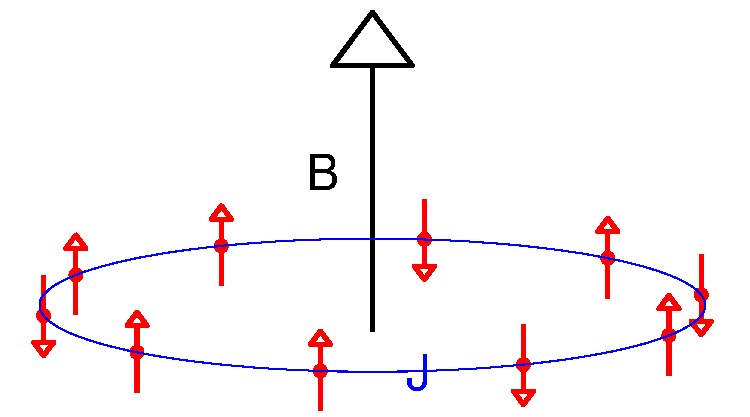
\includegraphics[width=7.5cm]{ising_spins}
 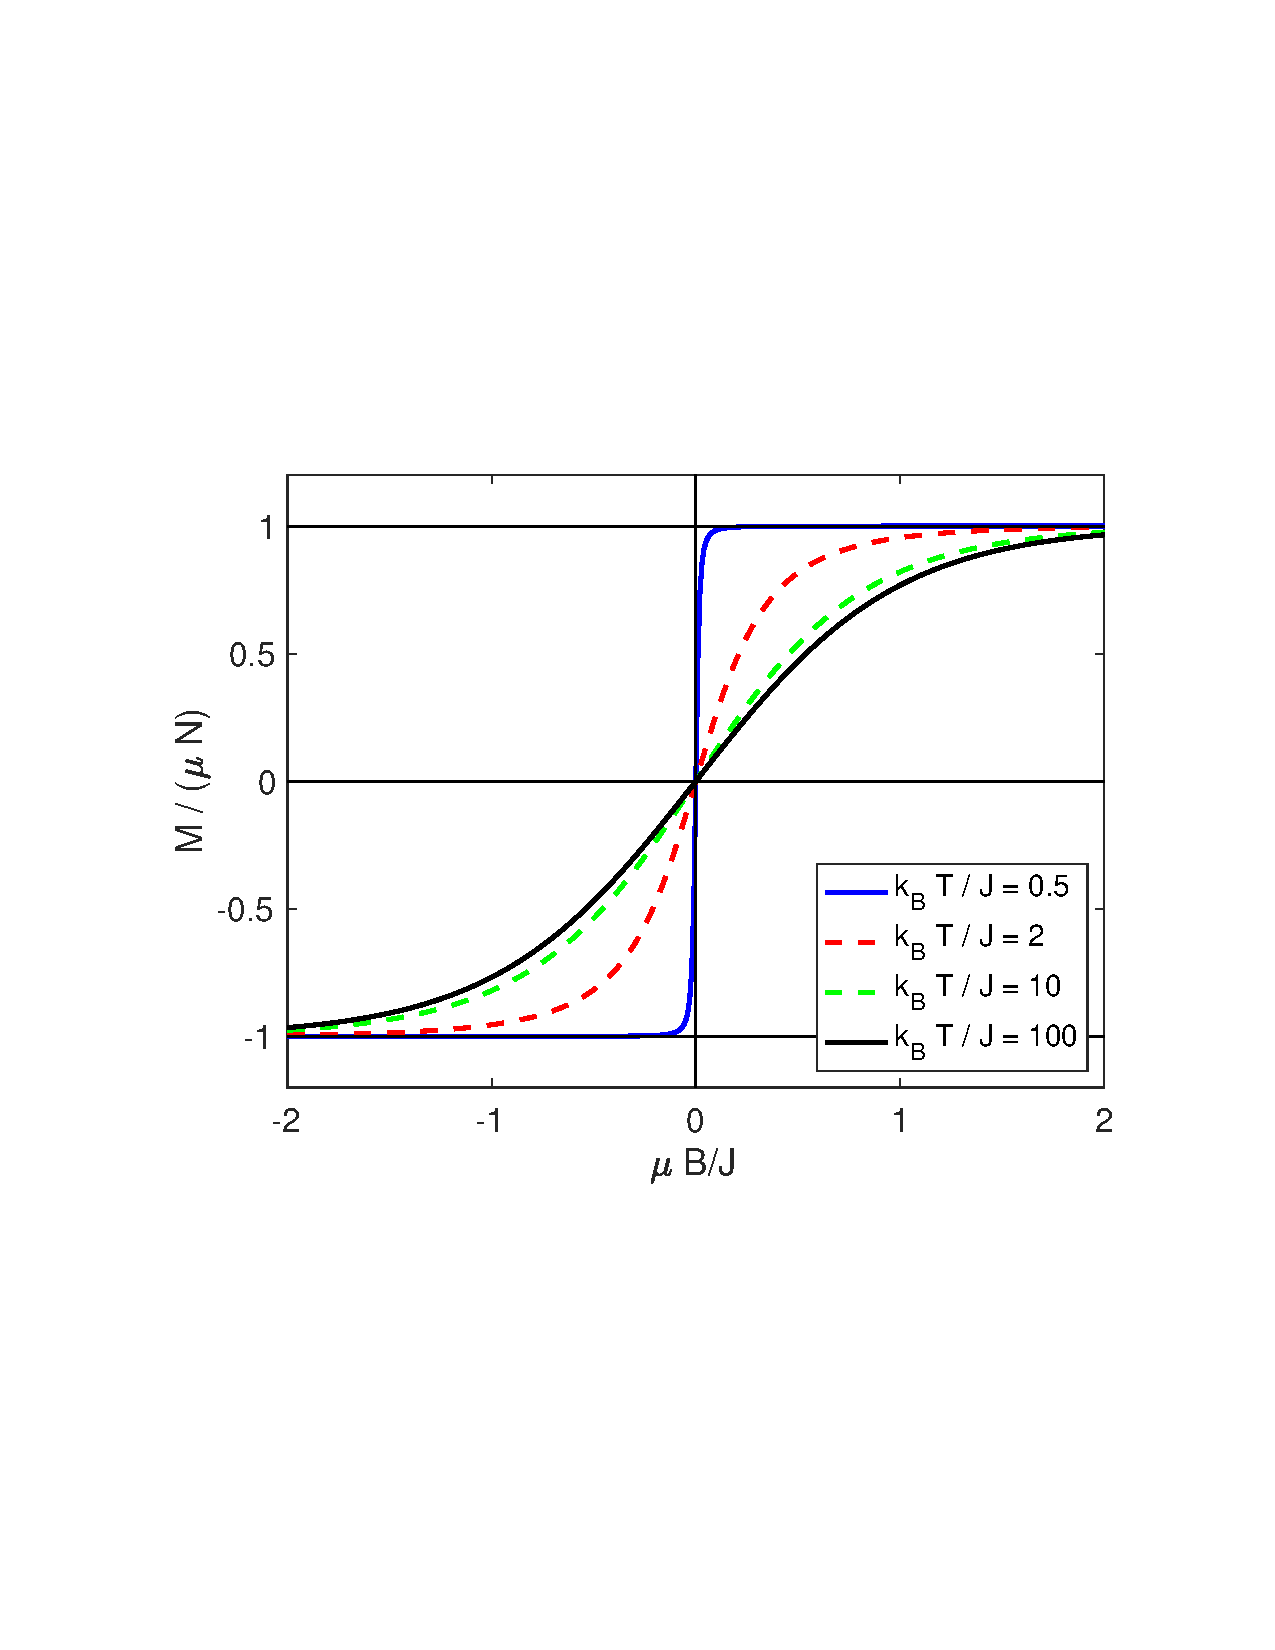
\includegraphics[width=7.5cm]{ising}\\[1.5cm]
$M(T,N,B) = N \mu \frac{\sinh(\mu \beta B)}{\sqrt{\sinh^{2}(\mu\beta B) + e^{-4 J \beta}}}$
\\[2.5cm]}
\parindent = 0pt
\maketitle
\newpage
\setcounter{page}{1}
\pagenumbering{arabic}
%\pagenumbering{roman}
\tableofcontents

%
%
%
%
\chapter{Ising Model}\label{chap:ising}
%


\begin{figure}[h]
\begin{center}
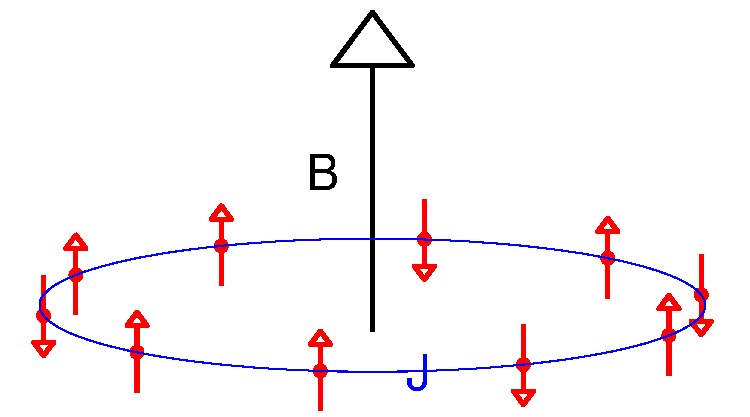
\includegraphics[width=5.5cm]{ising_spins}
\caption{{\it Arrangement of Ising-spins in a 1d chain with pbc.}}
\end{center}
\end{figure}
%



We will now examine collective magnetism.
The simplest model for this purpose is the Ising model, which is described by the following
Hamilton function 
%
\begin{align}
H &= - J \sum_{\langle i,j\rangle} S_{i} S_{j} - B \hat M\\
\text{with} \qquad \hat M &=  \mu \sum_{i} S_{i}\;,\qquad \bigg(\mu := - \frac{\mu_{B} g_{e}}{2}\bigg)\\
H&= - J \sum_{\langle i,j\rangle} S_{i} S_{j} - \mu B \sum_{i} S_{i}\;,
\end{align}
%
where the spins $S_{i}$ can only take the values  $S_{i}=\pm 1$.
$\mu_{B}$ is the Bohr magneton and $g_{e}$ the electronic Land\'e factor.
$J$ is the exchange coupling and the sum over sites is restricted to nearest neighbour sites, \red{such that each neighbouring pair is only counted once!}
$B$ stands for the magnetic flux density.
The Ising model is also used to describe binary alloys.
However, the parameters then have a different meaning.
The Ising model can be solved exactly in 1d and 2d and in $2d$ it even has a phase transition. 
We consider periodic boundary conditions \footnote{In most cases, boundary conditions are 
irrelevant in the  thermodynamic limits. } 

\section{Exact solution in 1D}
The Hamilton function of the Ising model in 1D reads
%
\begin{align*}
H &= - J \sum_{i=1}^{N} S_{i} S_{i+1} - \mu  B \frac{1}{2} \sum_{i} (S_{i}+S_{i+1})\\
\text{(pbc):}\qquad S_{i+N} &= S_{i}\;.
\end{align*}
%

\subsubsection{Canonical partition function}

The evaluation is particularly simply in the canonical ensemble:
\begin{align*}
Z(T,N,B) &= \sum_{\{S_{i}\}=\pm 1}\; e^{\beta J \sum_{ i} S_{i }S_{i+1} + \frac{\mu\beta B}{2} \sum_{i} (S_{i}+S_{i+1})}\\
 &= \sum_{\{S_{i}\}=\pm 1}\;
 \prod_{i=1}^{N}
  e^{j  S_{i }S_{i+1} + \frac{b}{2} (S_{i}+S_{i+1})}\;.
\end{align*}
%
We introduced the abbreviations $j = \beta J$ for the exchange coupling and $b = \mu B \beta$ for the magnetic flux density.
We also define the 
{\bf transfer matrix}
%
\begin{subequations}\label{eq:transfer:1d}
\begin{align}
{\cal T}_{s,s'} &:=   e^{j \; s s' + \frac{b}{2} (s + s')}\\
%
\text{which has the  matrix elements}\qquad
{\cal T}_{s,s'}&=
\begin{tabular}{c|ccc}   & +1 & -1 \\\hline+1 & $e^{j+b}$ & $e^{-j}$  \\-1 & $e^{-j}$ & $e^{j-b}$
\end{tabular}\\
%
\text{then:}\qquad Z(T,N,B)&= \sum_{\{S_{i}\}=\pm 1}\;
 \prod_{i=1}^{N} {\cal T}_{S_{i},S_{i+1}}\;.
\end{align}
\end{subequations}
%
We first consider the case $N=2$, where the partition function reads
%
\begin{align*}
Z(T,N=2,B) &= \sum_{S_{1}=\pm 1}\sum_{S_{2}=\pm 1}\;
{\cal T}_{s_{1},s_{2}}\;{\cal T}_{s_{2},s_{1}} = \sum_{s_{1}} \big({\cal T}^{2}\big)_{s_{1},s_{1}} = \tr{{\cal T}^{2}}
\end{align*}
%

The generalization to $N>2$ leads  obviously to
%
\begin{align*}
Z(T,N,B) &= \tr{{\cal T}^{N}}\;.
\end{align*}
%
The transfer matrix is real-symmetric and can be expressed in the spectral representation as follows
%
\begin{align*}
{\cal T} &= U D U^\dagger\;,
\end{align*}
%
here  $U$ is the unitary matrix of eigenvectors and  $D$ the diagoal matrix of eigenvalues
 $(d_{1},d_{2})$. Hence we have
%
\begin{align*}
Z(T,N,B) &= \tr{{\cal T}^{N}}= \tr{(U D U^{\dagger})^{N}} =\tr{U D^{N} U^{\dagger}} = \tr{D^{N}}\\
&= d_{1}^{N} + d_{2}^{N}\;.
\end{align*}
% 
The eigenvalues of the transfer matrix ate
%
\begin{align*}
d_{1/2} &= \frac{e^{j+b}+e^{j-b} }{2} \pm
\sqrt{ \bigg(
\frac{e^{j+b}-e^{j-b} }{2}
\bigg)	^{2} + e^{-2 j}}\\
&= e^{j} \bigg(\cosh(b) \pm \sqrt{\sinh^{2}(b) + e^{-4j}}\bigg)\\
\end{align*}
We can use $d_{1}>d_{2}$ in the calculation of the partition function  in thermodynamic limits
%
\begin{align*}
Z(T,N,B) &= d_{1}^{N}\bigg[
1 + 
\bigg(
\frac{d_{2}}{d_{1}}
\bigg)^{N}
\bigg]\;.
\end{align*}
%
%
\subsubsection{Free energy}
The free energy reads
%
\begin{align*}
F(T,N,B) &= -k_{B}T \Ln{Z(T,V)} = -k_{B}T N \ln(d_{1}) -k_{B} T 
\Ln{1+\underbrace{\bigg(
\frac{d_{2}}{d_{1}}
\bigg)^{N}}_{\to 0}} \\
&= - N k_{B}T\ln(d_{1})\;.
\end{align*}
%
\subsubsection{Magnetization}

The mean magnetization is
%
\begin{align*}
M &= \mu \; \langle\sum_{i} S_{i}\rangle\;.
\end{align*}
% 
The comparison with the partition function immediately shows
%
\begin{align*}
M &=  \frac{1}{\beta} \left(\frac{\partial \ln(Z)}{\partial  B}\right)\bigg|_{T,N } = -
 \left(\frac{\partial F}{\partial  B}\right)\bigg|_{T,N } \\
 &= - \mu \beta \left(\frac{\partial F}{\partial  b}\right)\bigg|_{T,N } \\
 &= - \mu \beta (-k_{B} T N) \left(\frac{\partial \ln(d_{1})}{\partial  b}\right)\bigg|_{T,N } \\
 &= N \mu  \frac{\frac{\partial d_{1}}{\partial  b}}{d_{1}} 
 =N \mu \frac{\sinh(b) + \frac{\sinh(b) \cosh(b)}{\sqrt{\sinh^{2}(b)+e^{-4j}}}}{\cosh(b) + \sqrt{\sinh^{2}(b)+e^{-4j} }}\\
 &=N\mu \sinh(b)\;\frac{1 + \frac{\cosh(b)}{\sqrt{\sinh^{2}(b)+e^{-4j}}}}{\cosh(b) + \sqrt{\sinh^{2}(b)+e^{-4j} }}\\
 &=N \mu\frac{\sinh(b)}{\sqrt{\sinh^{2}(b)+e^{-4j}}}\;\frac{\sqrt{\sinh^{2}(b)+e^{-4j}} + \cosh(b)}{\cosh(b) + \sqrt{\sinh^{2}(b)+e^{-4j} }}\;.
\end{align*}
%
%
\tboxit{Magnetization of the 1d Ising model}{
\begin{align*}
M(T,N,B) &= N \mu \frac{\sinh(\mu \beta B)}{\sqrt{\sinh^{2}(\mu\beta B) + e^{-4 J \beta}}}\;.
\end{align*}
}
%?


\subsection{Paramagnet}

Without interaction of the magnetic moments  ($J=0$) we obtgain
\begin{align*}
M(T,N,B) &= N \mu \frac{\sinh(\mu \beta B)}{\sqrt{\sinh^{2}(\mu\beta B) + 1}}
= N \mu \tanh(\mu\beta B)\;,
\end{align*}
%
the well-known result for paramagnetism.


\subsection{Limits}

It depends on the order of the limits. If we first set $B=0$, we obtain for any finite temperature
%
\begin{align*}
M(T,N,B=0) &= 0
\end{align*}
%
a vanishing magnetization, since $\sinh(\mu\beta B)$ always yields $0$ indepedent of $\beta$.
In the opposite order, i.e. keeping $B>0$ finite and let  $T$ go to zero, i.e.$\beta\to\infty$ we obtain
%
\begin{align*}
M(T,B\ne 0) &=
N \mu \frac{\sinh(\mu \beta B)}{\sqrt{\underbrace{\sinh^{2}(\mu\beta B)}_{\gg 1} + \underbrace{e^{-4 J \beta}}_{\ll 1}}}\\
&\underset{T\to 0}{\longrightarrow} \;N \mu\; \frac{\sinh(\mu\beta B)}{\pm\sinh(\mu\beta B)} \\
&= \;N \mu\;\text{sign}(B)\;.
\end{align*}
%
In this limiting  case we get perfect alignment of all spins, even if we now let $B$ go to zero. 
\nboxit{blue}{The Ising model in one dimension
has a "phase transition" at $T=0$.}	

\pagebreak
\subsection{Magnetization}


We use the exchange coupling $J$ as  energy unit. Then two independent parameters remain, $k_{B}T$ and $\tilde B: = \mu B$. We plot magnetization as a function of $\tilde B$
\begin{figure}[h]
  \centering
  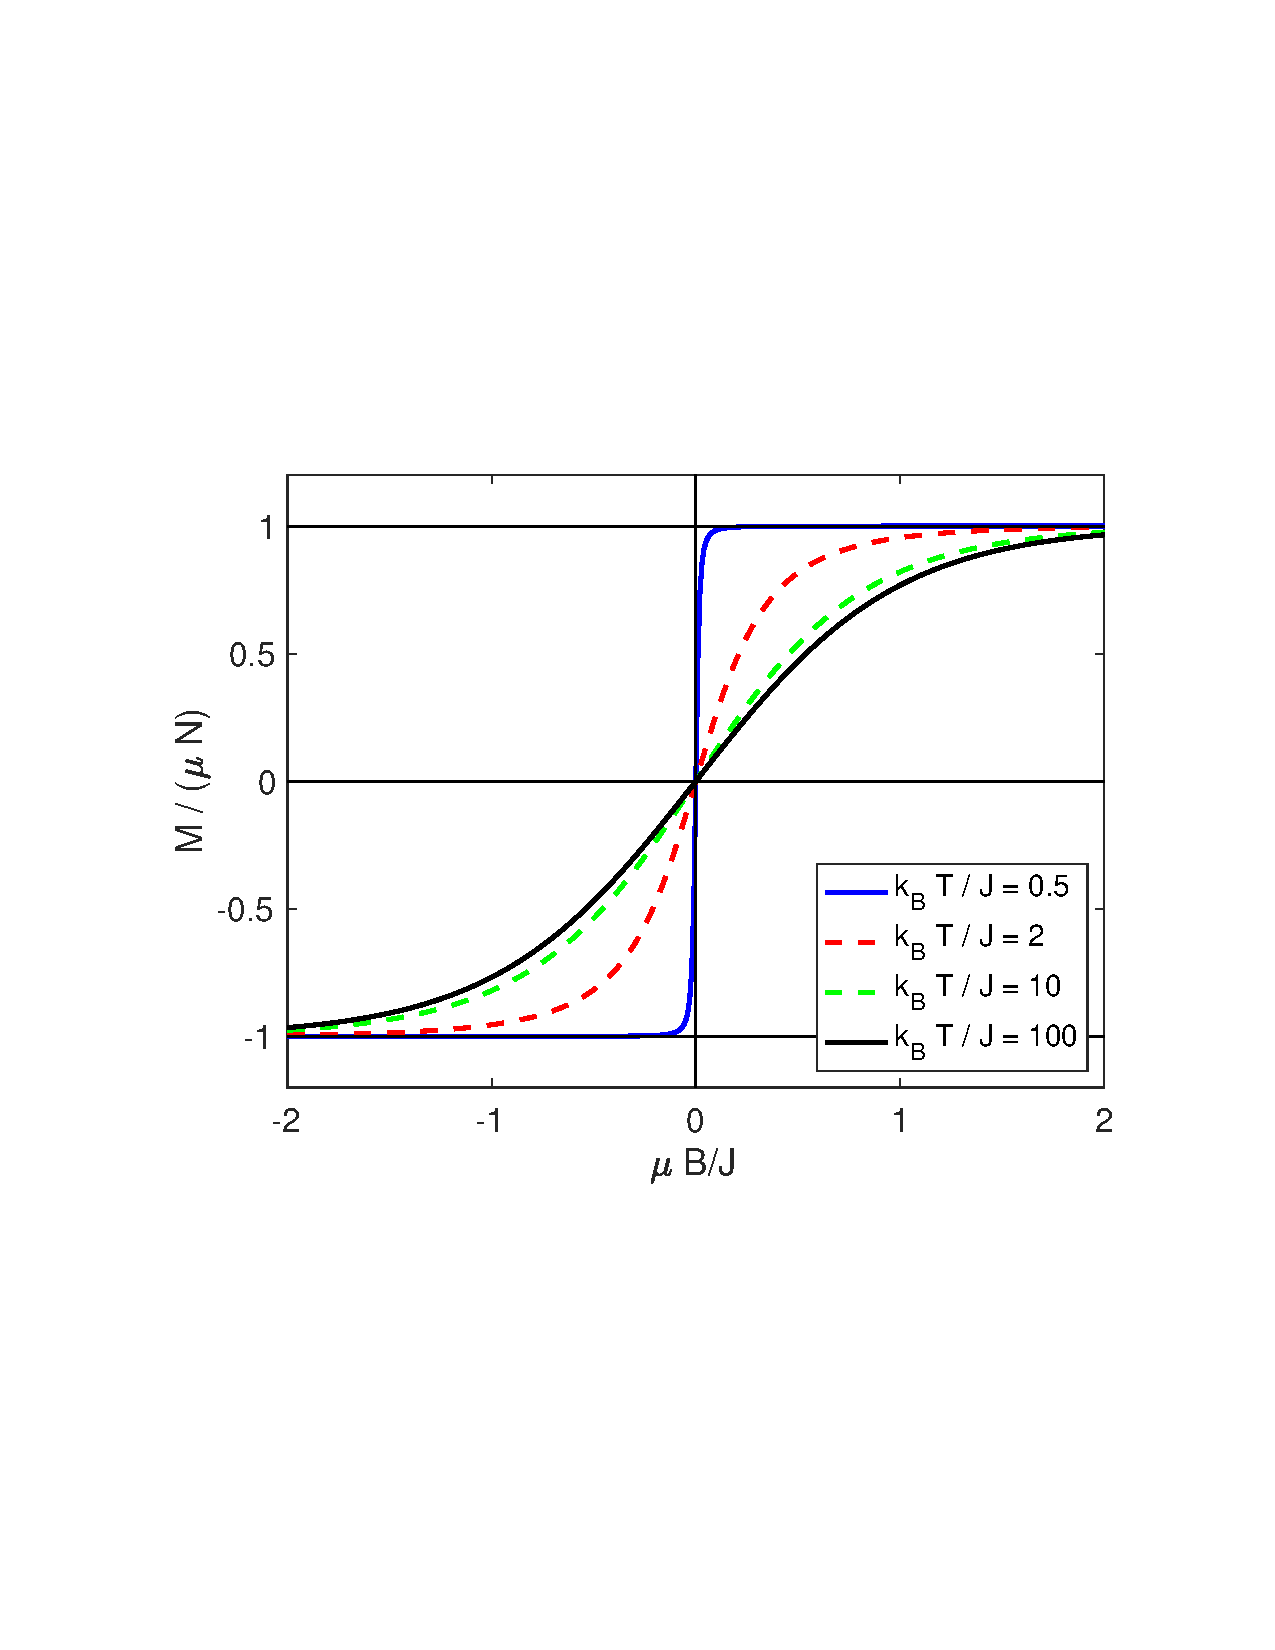
\includegraphics[width=10cm]{ising}
  \caption{Magnetization curve of the 1d Ising model.}
\end{figure}

We can see from the comparison with the result for the paramagnet that the amount of magnetization increases everywhere due to the influence of the interaction. For low temperatures, the magnetization abruptly enters the fully polarized state.

\section{Mean field approximation for any dimension}

(See {\em Ising Model for Magnetism (Springer)})

We will study the concept of the mean-field approximation in terms of the Ising model. 
We start out from  the Ising model expressed as
%
\begin{align*}
H &= - J \sum_{\langle ij\rangle} S_{i}S_{j} - 
B \cdot \hat M
\end{align*}
%
We recall that the Ising model describes spin-$1/2$ objects. 
The total magnetisation $\vv M$ is related to the spins
via 
%
\begin{align*}
\hat  M &=  \mu \sum_{i}
S_{i}\;.
\end{align*}
%
Now the Ising model takes only the component along the quantization axis into account and $S_{i}^{z}$ takes the values $\frac{\hbar}{2} \sigma_{i}$, with 
	$\sigma_{i}\in \{-1,+1\}$. 
%
As before, we introduce the  variable
%
\begin{align*}
h &= \mu  B\;.
\end{align*}
%
and obtain
\begin{align*}
H &= -J \sum_{\langle ij\rangle} S_{i}S_{j} - 
h \sum_{i} S_{i}
\end{align*}
Which is precisely the Hamiltonian of the Ising model. The mean field approximation is defined for any two dynamical variables $A$ and $B$
by
%
\begin{align*}
A B &\approx \langle A  \rangle B + A \langle B \rangle
-\langle A \rangle\langle B  \rangle\;.
\end{align*}
%
In our case, assuming translational invariance, we have
\begin{align*}
S_{i} S_{j}&\approx \langle S \rangle S_{j} + S_{i} \langle S \rangle
-\langle S \rangle^{2}\;.
\end{align*}
This leads to  the mean-field Hamilton function
%
\begin{align*}
H_\text{MFA} &= - J  \sum_{\langle ij\rangle}  \langle S \rangle S_{i}
- J  \sum_{\langle ij\rangle}  \langle S \rangle S_{j}
+J \sum_{\langle ij\rangle}  \langle S \rangle^{2}
  - h
\sum_{i} S_{i} \\
&= - 2J    \langle S \rangle \sum_{\langle ij\rangle} S_{i}
+J \sum_{\langle ij\rangle}  \langle S \rangle^{2}
  - h \sum_{i} S_{i} \\
\end{align*}
%
Since we have used the convention that the sum over nearest neighbours avoids
double counting, each site $i$ has $z/2$ nearest neighbours, where for simple cubic lattices $z=2d$ is defined as the total number of nearest neighbours.
Hence:
%
\begin{align*} %TODO: Added factor 1/2 here, is it correct?
H_\text{MFA} 
&= - J z  \langle S \rangle \sum_{i}  S_{i}
+ \frac{J N z}{2}  \langle S \rangle^{2}
  - h
\sum_{i} S_{i} \;.
\end{align*}
%
%
This can also be written as
\begin{align}\label{eq:ising:H:mfa}
H_\text{MFA} &=
  - h '\sum_{i} S_{i}
+ \frac{J N z}{2}  \langle S \rangle^{2}
 \\
\text{with }\qquad h' &= h + Jz \langle S \rangle\;.
\end{align}
The canonical partition function is then given by
%
\begin{align}\label{eq:ising:mfa:aux1}
Z(T,N,B) &= e^{-\frac{ \beta N J z}{2}\langle S \rangle^{2}} \sum_{\{S_{i}\}} e^{\beta h'\sum_{i}S_{i}}\;,
\end{align}
%
The partition function can easily be computed
%
\begin{align}\label{eq:}
Z(T,N,B) &= e^{-\frac{\beta N J z}{2} \langle S \rangle^{2}}\prod_{i} \sum_{S_{i}=\pm 1} e^{h' S_{i}} \nonumber\\
&= \bigg(  e^{\frac{-\beta J z}{2} \langle S \rangle^{2}}2 \cosh(\beta h') \bigg)^{N}\\
\ln\big( Z(T,N,B)  \big)
&= N \bigg( -\frac{\beta J z}{2} \langle S \rangle^{2} 
+\ln(2) 
+\ln\big( \cosh(\beta h')   \big) 
\bigg)
\label{eq:Z:Ising:MFA}
\end{align}
%
\subsection{Magnetization}
Next we compute the mean total spin ${\cal S}:=\sum_{i}S$
%
\begin{align*}
\avg{\cal S}
&=\frac{1}{Z}\sum_{\{S_{i}\}} 
\left\{ 
{\cal S} e^{-\frac{\beta N J z}{2}\langle S \rangle^{2}} e^{\beta h' {\cal S}}
\right\}
= \frac{k_{B}T}{Z} \frac{\partial }{\partial h'} Z\;.
\end{align*}
%
Hence
%
\begin{align}\label{eq:}
\avg{\cal S} &=k_{B}T\frac{\partial \ln(Z)}{\partial h'}
= N \tanh(\beta h')\;.
\end{align}
We introduce as $m$ the magnetization per site, divided by $\mu$
%
\begin{align}
m &= \frac{M}{\mu N} = \frac{1}{N}\langle\sum_{i}S_{i}  \rangle = \langle S \rangle\;.
\end{align}
%
%
and obtain the equation of state by using $h' = h + J z \langle S \rangle $ and dividing by $N$:
\tboxitp{Magnetization}{of the Ising model}{
%
\begin{align}\label{eq:eos:ising}
m &= \tanh\bigg( \beta \big(J z m + h\big)\bigg)\;.
\end{align}
%
}
We are particularly interested in the spontaneous magnetization, i.e. the magnetization for
$B\to 0 \Rightarrow h\to 0$. So we seek the solution of
%
\begin{align}\label{eq:magnetization:mfa}
m &= \tanh\big( \beta J z m\big)\;.
\end{align}
%
We introduce an auxiliary  temperature $T^{*}$, defined by
%
\begin{align}\label{eq:}
k_{B}T^{*} &= J z\;.
\end{align}
%
The condition for the spontaneous magnetization can therefore be expressed in a form and independent of the dimension
%
\begin{align}\label{eq:ising:mfa:mag}
m &=\tanh\big( \frac{T^{*}}{T} m \big)
\end{align}
%
or rather with $x = \frac{T^{*}}{T}m$
\begin{align}\label{eq:magnetization:mf}
x &= \frac{T^{*}}{T} \tanh\big( x \big)\;.
\end{align}
The function $\tanh(x)$ starts at $x=0$ with the value $0$ and slope 1, then it increases monotonically with  decreasing slope and approaches $1$ for $x\to \infty$.  
\eq{eq:magnetization:mf} has always the trivial solution $x=0 \Leftrightarrow  M=0$. For the non-trivial solution,
we need $\frac{T^{}*}{T}>1$, or rather $T<T^{*}$. According to the behaviour of $\tanh(x)$, for $\frac{T^{}*}{T}> 1$ there is precisely one non-trivial solution.
So we see that $T^{*}$ is indeed the critical/ Curie temperature, i.e
%
\begin{align}\label{eq:}
k_{B} T_{C}&=J z\;.
\end{align}
%

In 2D, we have $(\beta_{c} J)=.25$, as compared to the exact value $\beta_{c}J=0.4407$.
This not so bad, however, for 1D the mean-field result predicts a phase-transition at $(\beta_{c} J)=.5$, while the exact result is $\infty$.

In figure \ref{fig:M:mfa:ising}, the magnetization, obtained from \eq{eq:magnetization:mfa}, is depicted as function of $T$. Interestingly, the curve is independent of the spatial dimension.
The latter only enters in the value of $T_{c}$
\begin{figure}[t]
\begin{center}
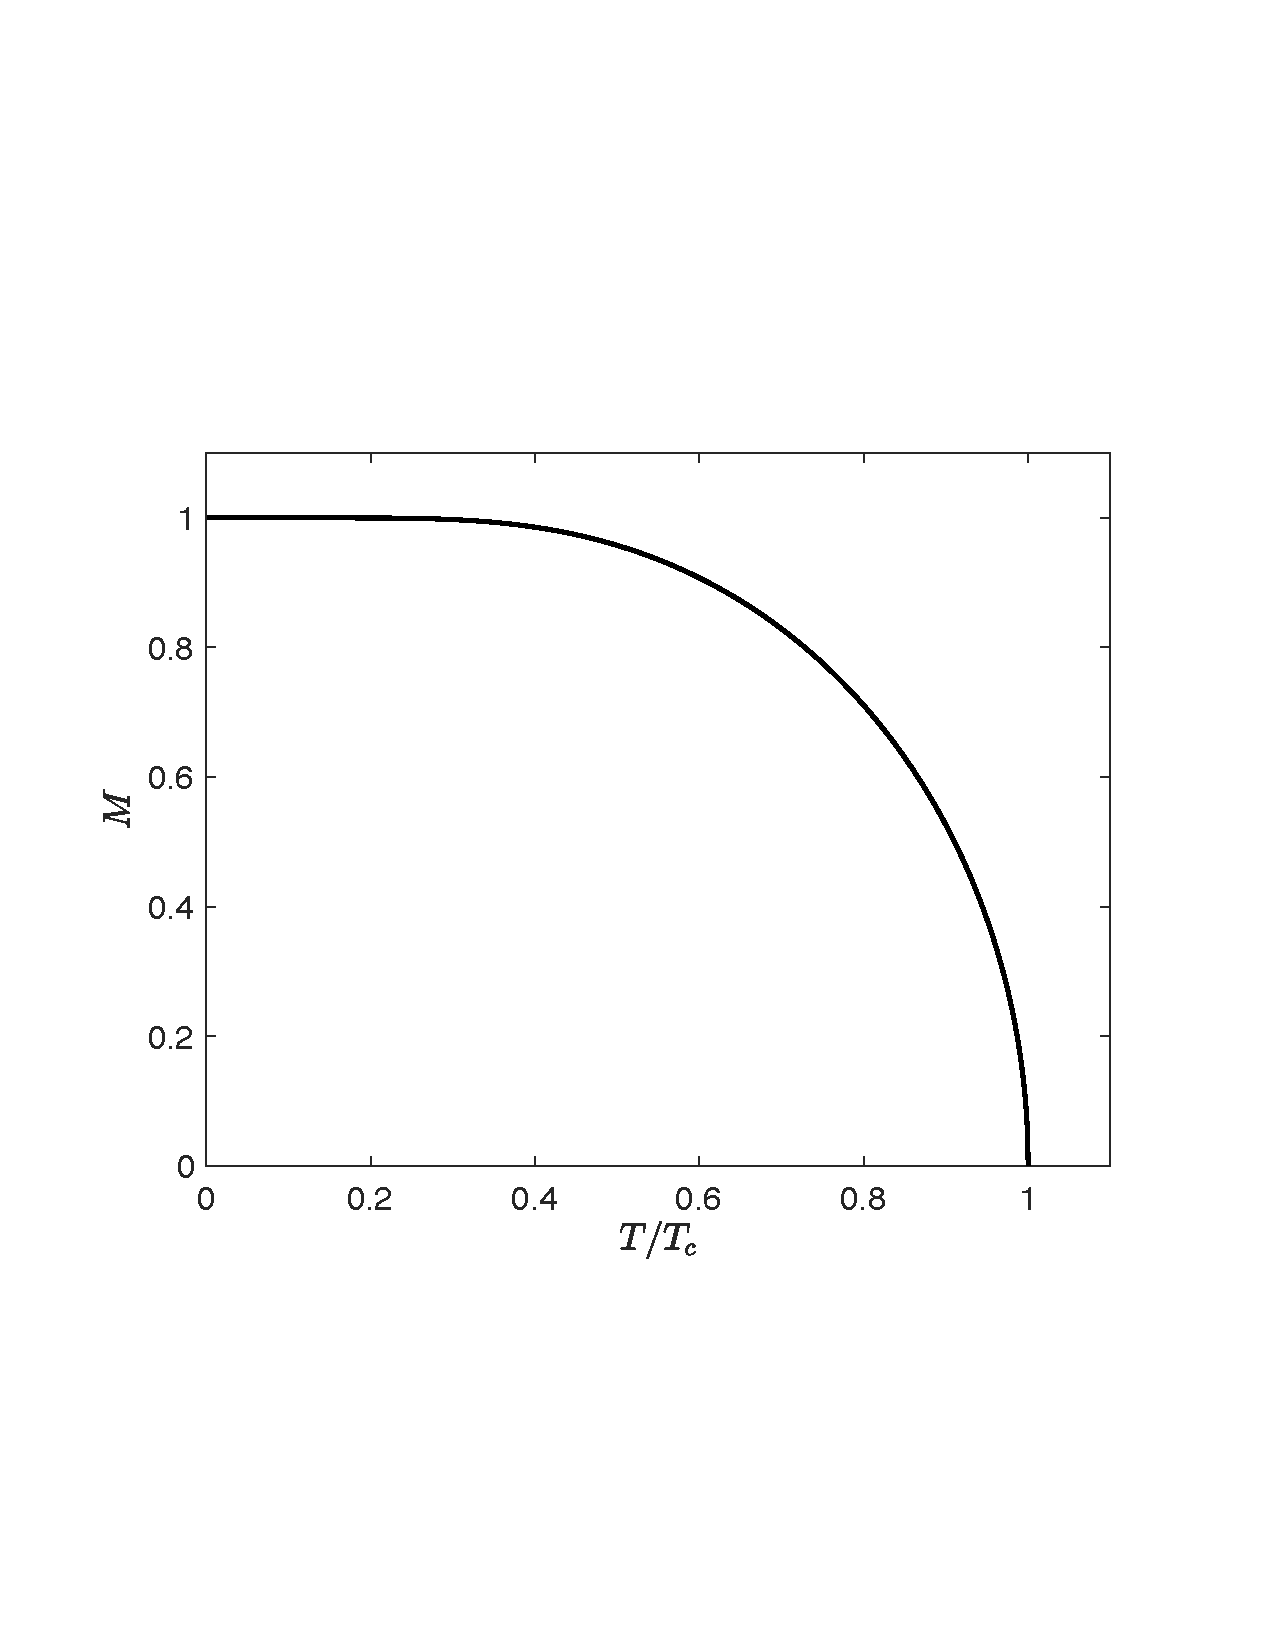
\includegraphics[width=7.5cm]{M_mfa_ising}
\caption{\it Mean-field result for the Magnetization for arbitrary spatial dimension $d$\label{fig:M:mfa:ising}}
\end{center}
\end{figure}

\subsubsection{Critical exponent}
For temperatures $T$ slightly below $T_{c}$, the magnetization is very small and we can use the Taylor expansion with $\tau = T/T_{C}$
\begin{align*}
m &= \tanh\big( \frac{m}{\tau} \big)= \bigg( \frac{m}{\tau} -\frac{(m/\tau)^{3}}{3} \bigg)
= \frac{m}{\tau}\bigg( 1- \frac{(m/\tau)^{2}}{3}\bigg)\\
\tau  &= 1 - \frac{(m/\tau)^{2}}{3}\\
\bigg(\frac{m}{\tau}\bigg)^{2} &= 3 \bigg( 1-\tau\bigg)\;.
\end{align*}

Up to this order we have for $T<T_{C}$
%
\begin{align}\label{eq:ising:mfa:m:Taylor}
m&= 3\tau \sqrt{1- \tau} \propto \varepsilon^{\frac{1}{2}}\\
\varepsilon &:= \frac{T_{C}-T}{T_{C}}
\end{align}
%
The  critical exponent is therefore $\beta=1/2$. 


\subsection{Magnetic susceptibility} %TODO: left out T=0?

Starting from the definition of the susceptibility via
%
\begin{align*}
\chi &= \frac{\partial M}{\partial B}\bigg|_{T,h=0}
\end{align*}
%
we obtain with $M=m N\mu$ and $B=h/\mu$ the relation 
%
\begin{align*}
\chi &= \left[ \frac{\partial M}{\partial m} \frac{\partial h}{\partial B} \frac{\partial m}{\partial h}  \right]_{T,h=0} = \mu^{2} N\pder{m}{h}{T,h=0}
\end{align*}
We start out from 
%
\begin{align*}
m &= \tanh\big(\beta h  +  \frac{T_{C}}{T} m\big)
\end{align*}
%
The derivative w.r.t. $h$ is
%
\begin{align*}
\xi=\pder{m}{h}{T, h=0} &=
\frac{\beta + \frac{T_{C}}{T} \xi}{\cosh^{2}\big( \beta h  +  \frac{T_{C}}{T} m \big)}\bigg|_{h=0}=
\frac{\beta + \frac{T_{C}}{T} \xi}{\cosh^{2}\big(\frac{T_{C}}{T} m \big)}\\
\xi \cosh^{2}\left(\frac{T_{C}}{T} m \right) &= \beta+ \frac{T_{C}}{T} \xi \\
\xi\bigg( \cosh^{2}\left(\frac{T_{C}}{T} m \right) - \frac{T_{C}}{T} \bigg) &= \beta\;.
\end{align*}
%
Close to $T_{C}$ the magnetisation is very small and we can Taylor expand the magnetisation
resulting in
%
\begin{align*}
\xi &= \frac{\beta}{ \cosh^{2}\big(\frac{T_{C}}{T} m \big) - \frac{T_{C}}{T} }\\
 &= \frac{\beta}{ 1 - \frac{T_{C}}{T} + \big( \frac{T_{C}}{T} m \big)^{2}}\\
 &= \frac{1}{k_{B}}\;\frac{1}{ T - T_{C}+  T_{C} \frac{T_{C}}{T} m^{2} }\;.
\end{align*}
%
We can replace $T$ by $T_{C}$ in the last term in the denominator, as it already contains $O(m^{2})$
%
\begin{align*}
\xi &= \frac{1}{k_{B}}\;\frac{1}{ T - T_{C}+  T_{C}  m^{2} }\;.
\end{align*}
%
{\bf For $T\searrow T_{C}$} the magnetisation is zero and we have 
\begin{align*}
\xi &= \frac{1}{k_{B} T_{C}} \;\big(\varepsilon\big)^{-1}
\end{align*}
with $\varepsilon=(T-T_{C})/T_{C}$.

\noindent
{\bf For $T\nearrow T_{C}$}  
we use  \eq{eq:ising:mfa:m:Taylor} for $m$ and obtain 
%
\begin{align*}
m^{2} &= 3 \tau^{2}\big( 1-\tau \big) = \frac{3}{T_{C}} \big( T_{C}-T \big) + {\cal O}(\Delta T/T_{C})^{2}
\end{align*}
%
and have
%
\begin{align*}
\xi &= \frac{1}{k_{B}}\;\frac{1}{ T - T_{C}+ 3  \big( T_{C}-T \big) }
= \frac{1}{2 k_{B}T_{C}}\abs{\varepsilon}^{-1}
\end{align*}
According to the definition of the critical exponent of the susceptibility 
%
\begin{align*}
\chi \simeq A_{\pm } \abs{\varepsilon}^{-\gamma_{\pm}}
\end{align*}
%
we have $A_{+}= 2 A_{-}$ and $\gamma_{+}=\gamma_{-}=1$.
%
\subsection{Free energy}
Next we compute the free energy based \eq{eq:Z:Ising:MFA}
%
\begin{align*}
f:=\frac{F}{k_{B} N} &=-\frac{k_{B}T}{k_{B} N} \ln(Z)\\
&=-T \bigg( -\frac{\beta J z}{2} \langle S \rangle^{2} 
+\ln(2) 
+\ln\big( \cosh(\beta h')   \big) 
\bigg)\\
%&=- T 
%\bigg[
%\frac{- \beta J z}{2} m^{2}  +
%\ln\big(2\cosh(\beta h + \frac{Jz}{k_{B}T}m)  \big)\bigg]\\
&=
\frac{J z}{2 k_{B}} m^{2}  - T
\ln\big(2\big)  - T\ln\big( \cosh(\beta h + \frac{J z}{k_{B}T} m)\big)\;.
\end{align*}
%
The natural variables are  $T$, $N$, and $h$.
However, we will see that the magnetization $m$ is more suitable than $h$ and we will
introduce a corresponding Legendre transformation later.

We have seen before that $k_{B} T_{C} = J z$ so we can 
express the free energy as
%
\begin{align*}
\frac{F}{N k_{B}} &= \frac{1}{2} T_{c} m^{2}
-  T\ln\big(2\big) - T\ln{ \cosh(\beta h + \frac{T_{c}}{T} m)  }\;.
\end{align*}
%
Along with
%
\begin{align*}
\cosh(x) &= \big(1-\tanh^{2}(x)\big)^{-1/2} 
\end{align*}
and the self consistency \eq{eq:ising:mfa:mag}
%
\begin{align}\label{eq:magnetization}
m &= \tanh\big( \beta h + \frac{T_{C}}{T} m \big)
\end{align}
%
we can express the free energy as
%
\begin{align}\label{eq:isingh:mfa:F}
\frac{F}{N k_{B}} &= \frac{T_{c} m^{2}}{2} 
-  T\ln\big(2\big)  + \frac{T}{2} \ln\big(1-m^{2}\big)\;.
\end{align}
%

Next we compute the Helmholtz free energy, by the following Legendre transform, where we introducing $M$ as  natural variable instead of $h$:
%
\begin{align}
A(T,M) &= F(T,h) + Mh\;.
\end{align}
%
Then the total differential reads
%
\begin{align*}
dA  &= dF(T,h) + h dM +M dh\\
&= -S dT - M dh + h dM +M dh  \\
&= -S dT + h dM\;.
\end{align*}
%
\blue{exercise: proof  $\frac{\partial F}{\partial h}= - M $ by using \eq{eq:isingh:mfa:F} and \eq{eq:magnetization}.}
Hence 
%
\begin{align}\label{eq:MFA:dA:dM}
\pder{A}{M}{T} &= h\\
\pder{A}{T}{M} &= -S\;.\label{eq:MFA:S}
\end{align}
%
%
If we want to have spontaneous magnetisation,  i.e. a finite magnetisation $M$
without external field, then according to \eq{eq:MFA:dA:dM} we are looking for 
a finite value of the magnetization $M$ for which
%
\begin{align}\label{eq:MFA:dA:dM:zero}
\pder{A(M,T)}{M}{T} &= 0\;.
\end{align}
%
Before we can exploit this equation, we need to express $h$ in  terms of $M$ (or rather $m$).
To this end we invert 
%
\begin{align*}
m &= \tanh\bigg(\beta h + \frac{T_{C}}{T} m\bigg)
\end{align*}
%
leading to
%
\begin{align*}
\beta h + \frac{T_{C}}{T} m  &= \tanh^{-1}\big(m\big)\;.
\end{align*}
%
Along with 
\begin{align*}
\text{tanh}^{-1}\big(b\big)=\frac{1}{2}\ln\bigg( \frac{1+b}{1-b} \bigg)
\end{align*}
we obtain
%
\begin{align*}
\beta h +\frac{T_{c}}{T}m &= 
\frac{1}{2}\ln\bigg( \frac{1+m}{1-m} \bigg)\\
h &= \frac{k_{B}T}{2}\ln\bigg( \frac{1+m}{1-m} \bigg)
-k_{B}T_{c} m
\end{align*}
%
Then we obtain for the Helmholtz free energy of \eq{eq:isingh:mfa:F}
%
\begin{align*}
\frac{A}{N k_{B}} &= \frac{T_{C} m^{2}}{2} -T\ln(2) +\frac{T}{2} \ln\big( 1-m^{2} \big) + \frac{mh}{k_{B}}\\
 &=\frac{1}{2} T_{c} m^{2}
-  T\ln(2) + \frac{T}{2}\ln\big(1-m^{2} \big)
+ \frac{m }{k_{B}}
\bigg( \frac{k_{B}T}{2} \ln\bigg( \frac{1+m}{1-m} \bigg)
- k_{B}T_{c}m
\bigg)\\
 &=\frac{1}{2} T_{c} m^{2}
-  T\ln(2) + \frac{T}{2}\ln\big(1-m^{2} \big)
+
\frac{m T}{2}\ln\bigg( \frac{1+m}{1-m} \bigg)
- T_{c} m^{2}
\;.
\end{align*}
%
or rather
%
\begin{align}\label{eq:sing:mfa:S}
\frac{A}{N k_{B} T_{c}}= \frac{A}{N J z}&=-\frac{1}{2} m^{2}
-\tau\ln(2) + \frac{\tau}{2}\bigg[\ln\big((1-m)(1+m) \big)
+ m \ln\bigg( \frac{1+m}{1-m} \bigg)\bigg]\notag\\
&=-\frac{1}{2} m^{2}
-\tau\ln(2) + \frac{\tau}{2}
\bigg( 
\big(1+m\big) \ln\big(1+m \big) + \big(1-m\big) \ln\big(1-m \big)
 \bigg)\;,
\end{align}
%
%
with $\tau =T/T_{c}$.
%
\begin{figure}[h]
\begin{center}
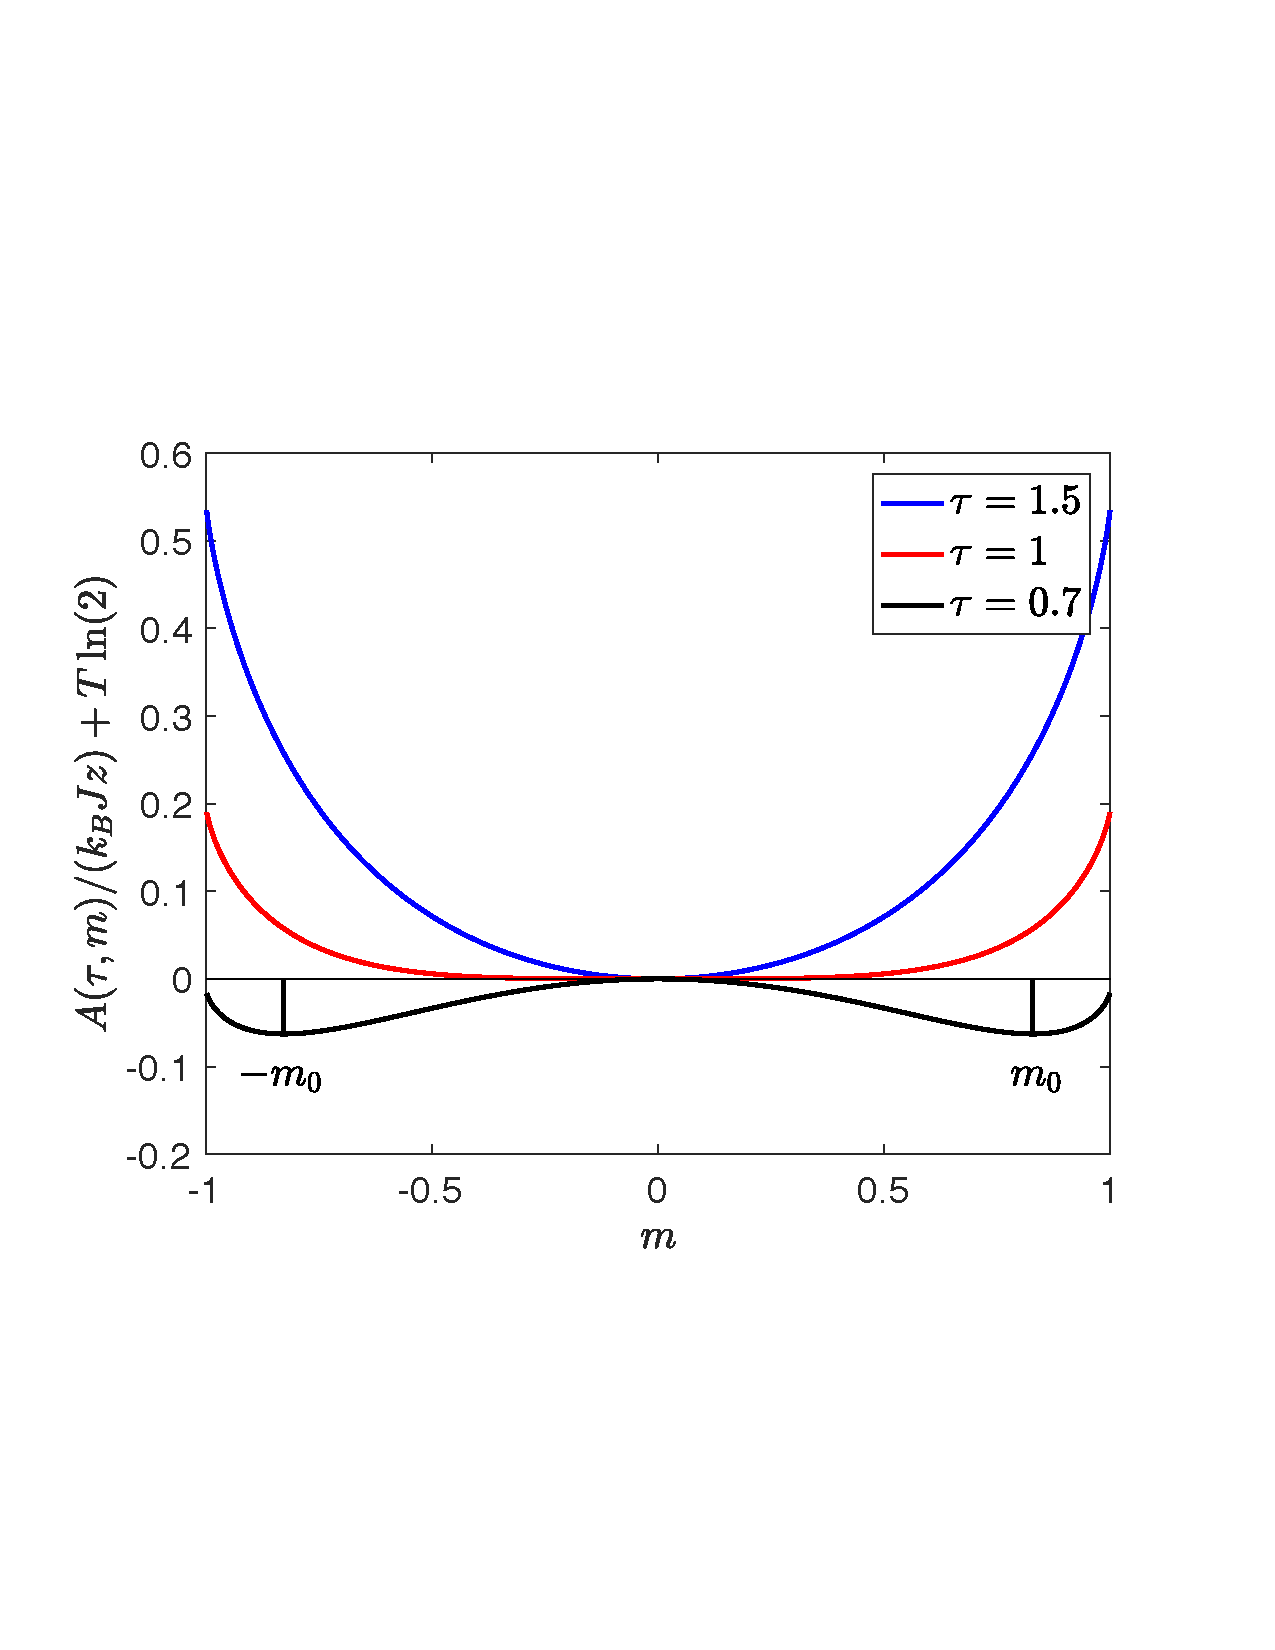
\includegraphics[width=7.5cm]{freeEnergyHemlholz}
\caption{{\it Helmholtz free energy for the Ising model in mean-field approximation versus order parameter without external field.}\label{fig:freeEnergyHemlholz}}
\end{center}
\end{figure}
%
According to \eq{eq:MFA:dA:dM:zero} the magnetization is given by the points where the slope as function of $m$ vanishes (see figure \ref{fig:freeEnergyHemlholz}).

\newpage 

\subsection{Entropy}


\begin{figure}[t]
\begin{center}
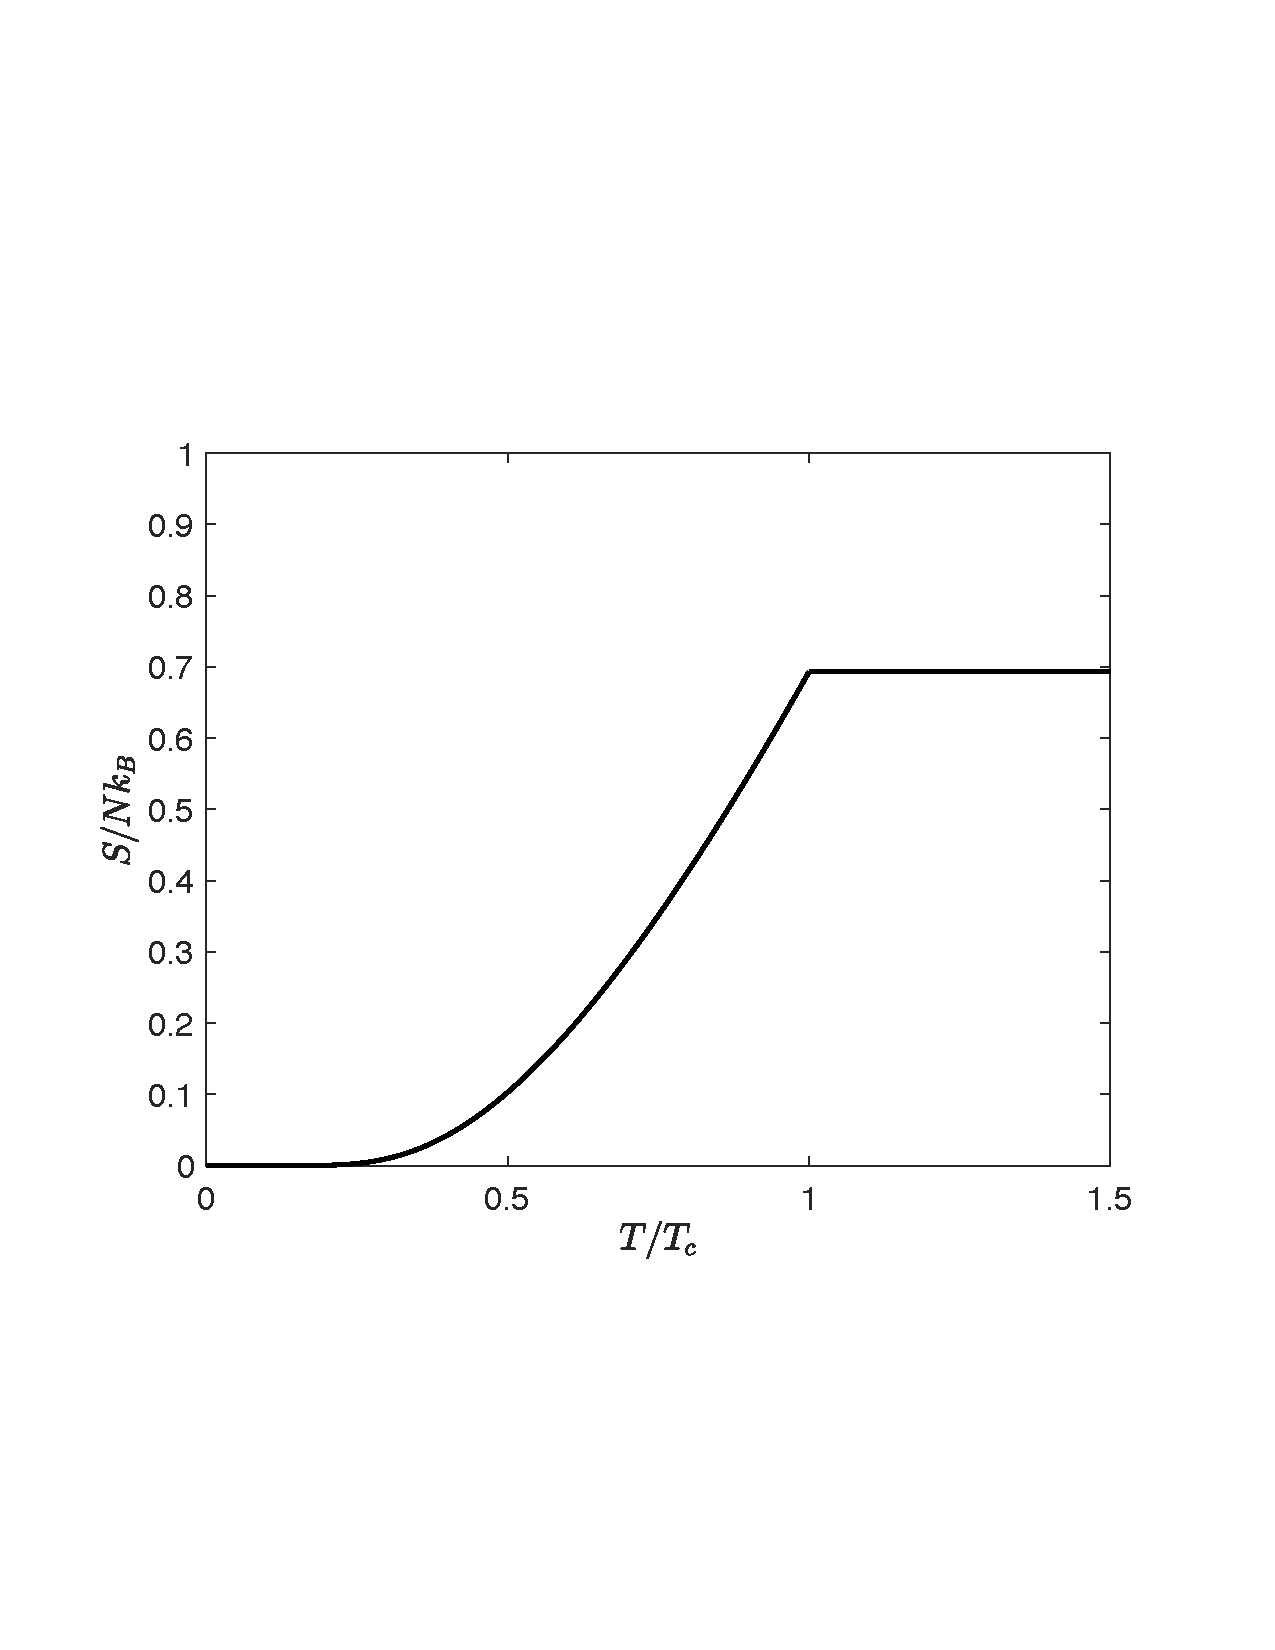
\includegraphics[width=7.5cm]{S_mfa_ising}
\caption{{\it Entropy of the Ising model in MFA.}}
\end{center}
\end{figure}

According to \eq{eq:MFA:S} , which was
%
\begin{align*}
S &= -\pder{A}{T}{M} 
\end{align*}
%
along with \eq{eq:sing:mfa:S}
the entropy is
%
\begin{align*}
-\frac{S}{N k_{B}T_{C}} &=
\frac{\partial }{\partial \tau} \bigg( 
-\frac{1}{2} m^{2}
-\tau\ln(2) + \frac{\tau}{2}
\bigg( 
\big(1+m\big) \ln\big(1+m \big) + \big(1-m\big) \ln\big(1-m \big)
 \bigg)
\bigg)\bigg|_{m} \frac{d \tau }{dT}\nonumber\;.
\end{align*}
%
Hence
%
\tboxitp{Entropy of the Ising model}{in MFA for zero field}{
\begin{align}
\label{eq:ising:mfa:entropy}
\frac{S}{N k_{B}}
&=
\ln(2) - \frac{1}{2}
\bigg(\big( 1+m \big)\ln\big(1+m\big) +
\big(1-m\big) \ln\big(1-m\big) \bigg)\;. 
\end{align}}
%

It has the correct limiting behaviour: For $T\to0$, i.e. $m\to 1$ we obtain
%
\begin{align*}
\frac{S}{N k_{B}} &= \ln(2) -\frac{1}{2}\bigg( 2\bigg( \ln(2) + 0 \bigg) \bigg) = 0\;,
\end{align*}
%
and for $T\to\infty$, i.e. $m\to 0$ the entropy becomes
%
\begin{align*}
\frac{S}{N k_{B}} &= \ln(2) -\frac{1}{2}\bigg( 
\ln(1) + \ln(1)  \bigg) = \ln(2)\;.
\end{align*}
%
Recall that
%
\begin{align*}
S &= k_{B} \ln( \text{number of micro states})\;.
\end{align*}
%
For $T\to \infty$ all states can be reach with the same probability. Hence the number of micro states is $2^{N}$ and
%
\begin{align*}
S &= N k_{B} \ln( 2)\;,
\end{align*}
%
in agreement with the above result.

For the entire $T$ dependence of $S$ we have to insert the self-consistent solution for $m(T)$ in \eq{eq:ising:mfa:mag}.
%
  \subsection{Internal Energy}
The internal energy is defined as the expectation value of the hamiltonian.
Using the mean field expression of \eq{eq:ising:H:mfa} we have
%
\begin{align*}
U &=
%\langle H \rangle = -h' \sum_{i} \langle S_{i} \rangle + \frac{J N z}{2} m^{2}=
 N\big(-h'  m + \frac{J  z}{2} m^{2}\big)
\intertext{with $ h' =J z m + h$ we obtain:} 
%&= -J z m^{2} - h m  + \frac{J  z}{2} m^{2}\\
\frac{U}{NJ }&= -\frac{h m }{J} - z m^{2} + \frac{z}{2}m^{2}\\
&= - \frac{z}{2} m^{2} - \frac{h m }{J}\;.
\end{align*}
%
For zero external field it simplifies to (we also use $z=2d$)
%
\tboxitp{Internal energy of the Ising model}{in MFA for zero field}{
\begin{align}
\frac{U}{NJ }&= - d\; m^{2} \;.
\end{align}}
%


\subsection{Specific heat}
For the specific heat we need
%
\begin{align*}
C_{h=0} &= \pder{U}{T}{h=0} = - d N J   \;\frac{d\; m^{2} }{d T} \\
\frac{C_{h=0}}{N J} &= -d\;   \;\frac{d }{d T}  m^{2}\;.
\end{align*}
%
Above $T_{C}$ the magnetization is zero and hence $C = 0$.
Slightly below $T_{C}$ we can replace $m$ by \eq{eq:ising:mfa:m:Taylor}, which gives

\begin{align*}
\frac{C_{h=0}}{N J} &= -d   \;\frac{d   }{d T}  3 \tau^{2}\big( 1-\tau \big)\\
&=- \frac{3d}{T_{C}^{3}}   \;\frac{d   }{d T}   \big( T^{2} T_{C}- T^{3} \big)\\
&=- \frac{3d}{T_{C}^{3}}   \;T\; \big( 2  T_{C}- 3 T \big)\;.
\end{align*}
Hence, approaching $T_{C}$ from below we obtain
%
\begin{align}\label{spec:heat:MFA}
\frac{C(T_{C})_{h=0}}{N J}
&= \frac{3d}{T_{C}} =  \frac{3d k_{B}}{J z} =\frac{3d k_{B}}{J 2d}\\
\frac{C(T_{C})_{h=0}}{N} &= \frac{3k_{B}}{2}\;.
\end{align}
%
Therefore, in MFA, the specific heat has no power-law behaviour close at $T_{C}$, but rather a 
discontinuity from $\frac{3}{2}k_{B}$ below $T_{C}$ to 0 above $T_{C}$.
For the entire $T$-dependence below $T_{C}$ we continue with
%
\begin{align}
\frac{C_{h=0}}{N J} &= - 2 d\;   m\;\frac{d m}{d T} \;.
\end{align}
%
First we consider
%
\begin{align*}
\xi :=\;\frac{d m}{d T}  \;.
\end{align*}
%
Exploiting \eq{eq:magnetization} yields
\begin{align}
\xi &= \frac{d}{dT} \tanh\big( \beta h + \beta k_{B} T_{C} m \big)\bigg|_{h=0}\\
\xi &= \frac{(h +  k_{B} T_{C} m )\frac{ d \beta}{dT} + \beta k_{B}T_{C} \xi}{\cosh^{2}\big( \beta (h +  k_{B} T_{C} m )\big)}\bigg|_{h=0}\\
 &= \frac{-\frac{T_{c}}{T^{2}}  m + \frac{T_{C}}{T} \xi}{\cosh^{2}\big( \frac{T_{C}}{T} m \big)}\;.
\end{align}
%
Then
%
\begin{align*}
\xi \cosh^{2}\big( \frac{T_{C}}{T} m \big) 
 &= -\frac{T_{c}}{T^{2}}  m + \frac{T_{C}}{T} \xi\\
\xi \bigg(\cosh^{2}\big( \frac{T_{C}}{T} m \big) -\frac{T_{C}}{T}\bigg)
 &= -\frac{T_{C}}{T^{2}}  m \\
\xi &= -\frac{1}{T_{C}}\;
\frac{\frac{m}{\tau}}{ \tau \cosh^{2}\big( \frac{m}{\tau} \big) - 1 }
\end{align*}
%
That leads to
%
\begin{align*}
\frac{C_{h=0}}{N J} &= - z\;   m\;\xi\\
&=\frac{z}{T_{C}} 
\frac{\frac{m^{2}}{\tau}}{ \tau \cosh^{2}\big( \frac{m}{\tau} \big) - 1 }\\
&=\frac{z}{z J/k_{B}} 
\frac{\frac{m^{2}}{\tau}}{ \tau \cosh^{2}\big( \frac{m}{\tau} \big) - 1 }\;.
\end{align*}
%
Finally, we have 
%
\begin{align}\label{eq:}
\frac{C_{h=0}}{N} &=k_{B 	}
\frac{\big(\frac{m}{\tau}\big)^{2}}{ \cosh^{2}\big( \frac{m}{\tau} \big) - 1/\tau }\;.
\end{align}
%
%
Together with the self consistent equation for $m(T)$:
%
\begin{align*}
m(T) &= \tanh\bigg(\frac{T_{C}}{T} m(T)\bigg)\;,
\end{align*}
%
which have solved numerically before, we can plot the specific heat.
\begin{figure}[t]
\begin{center}
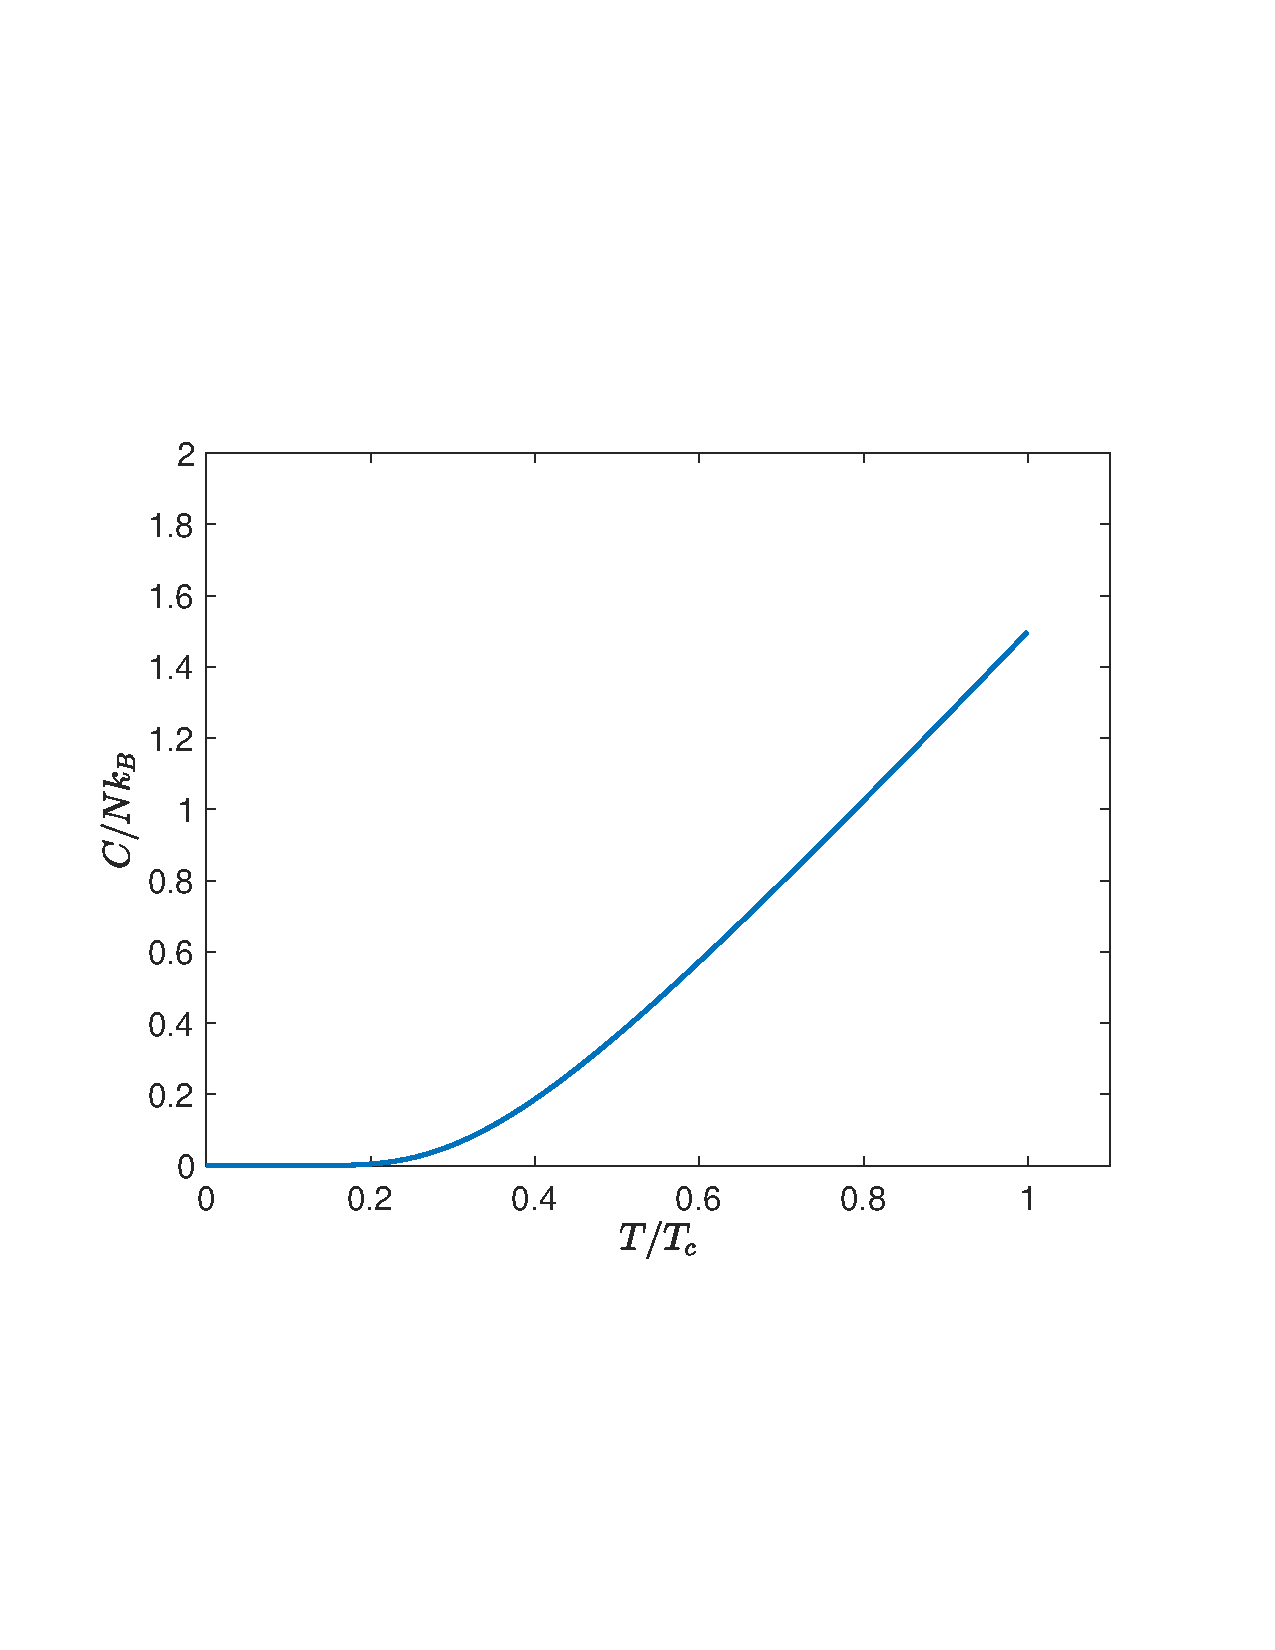
\includegraphics[width=7.5cm]{C_mfa_ising}
\caption{{\it Specific heat of the Ising model in MFA.}}
%TODO: Include also a plot of the internal energy in this
\end{center}
\end{figure}

We have seen in  'statistical physics I' 
%
\begin{align*}
C&= \frac{1}{k_{B} T^{2}} \avg{\big( \Delta H \big)^{2}}\;,
\end{align*}
%
i.e. $C$ is large when there are pronounced energy fluctuations,
which is the case in the vicinity of $T_{C}$.
In  MFA, above $T_{C}$ there are no fluctuations because
$H \propto m$ and therefore $U=0$ aboce $T_{C}$.
This is an artefact of MFA.


\section{Exact solution of the 2d Ising model}
\subsection{Transfermatrix approach}
We will first briefly explain how the Transfer matrix approach works in the 2d case.
To this end we will represent the hamiltonian of the 2d Ising model ($L_{x}\times L_{y}$)
by writing the two cartesian indices explicitly in the form
$S_{ij}$
%
%
\begin{align*}
-\beta H &= j \sum_{l=1}^{L_{y}} \sum_{i=1}^{L_{x}}	\qty( S_{i,l}S_{i+1,l} +S_{i,l}S_{i,l+1})
+ h \sum_{l} \sum_{i} S_{il}\;.
\end{align*}
%
Now we combine the spins of column $l$  (i.e. $S_{il}$) in a vector
%
\newcommand{\vS}[1]{{ \mathbf {\cal  S}^{(#1)}}}
\newcommand{\vSx}{{ \mathbf {\cal  S}}}
\newcommand{\vSp}{{ \mathbf {\cal  S}'}}
\begin{align*}
\vS{l} &= 
\begin{pmatrix}
S_{1,l}\\
S_{2,l}	\\
\ldots\\
S_{L_{x},l}
\end{pmatrix}\;,
\text{i.e. }(\vS{l})_{i} = S_{il}
\end{align*}
%
Then the hamiltonian can be written as
%
\begin{align}\label{eq:beta:H}
-\beta H &= \sum_{l}  A\big(\vS{l}, \vS{l+1}\big)\\
\intertext{with the definitions}
A(\vS{l},\vS{k}) &= \frac{1}{2}\bigg(\tilde A(\vS{l},\vS{k}) + \tilde A(\vS{k},\vS{l}) \bigg) \\
\tilde A(\vS{l},\vS{k}) &= 
j \sum_{i}  \bigg((\vS{l})_{i} (\vS{l})_{i+1}  +(\vS{l})_{i} (\vS{k})_{i}\bigg)
+ h \big(\sum_{i} \vS{l})_{i}\;.
\end{align}
%
$A$ is by construction a real symmetric matrix.
Inserting indices yields
%
\begin{align*}
\sum_{l} \tilde A(\vS{l},\vS{l+1}) &= 
 j \sum_{l,i}\big(  S_{i,l}S_{i+1,l} +S_{i,l}S_{i,l+1}\big)
+ h \sum_{i,l} S_{i,l} &&= - \beta H\\
\sum_{l} \tilde A(\vS{l+1},\vS{l}) &= 
 j \sum_{l,i}\big(  S_{i,l+1}S_{i+1,l+1} +S_{i,l+1}S_{i,l}\big)
+ h \sum_{i,l} S_{i,l+1} \\
(l+1 \to l'  \text{ plus pbc} \Rightarrow)\qquad 
&= j \sum_{l',i}\big(  S_{i,l'}S_{i+1,l'} +S_{i,l'}S_{i,l+1}\big)
+ h \sum_{i,l} S_{i,l'} &&= - \beta H\;.
\end{align*}
%
Hence \eq{eq:beta:H} is correct.
Then 
%
\begin{align*}
Z &= \sum_{\{S_{ij}\}} e^{\sum_{l=1}^{L} A(\vS{l},\vS{l+1}) }
 = \prod_{l=1}^{L} \sum_{\vS{l}}  e^{ A(\vS{l},\vS{l+1}) }\;.
\end{align*}
%
Now, we introduce the transfer matrix ${\cal T}$ with matrix elements
%
\begin{align*}
{\cal T}_{\vS{l},\vS{l'}} &= e^{A\big(\vS{l},\vS{l'}\big)}
\end{align*}
%
Then the partition function can be written as (remember that we use pbc)
%
\begin{align*}
Z &= \sum_{\vS{1}} \sum_{\vS{2}}\cdots  \sum_{\vS{L_{y}}}\prod_{l} {\cal T}_{\vS{l},\vS{l+1}}\\
&= \sum_{\vS{1}} \sum_{\vS{2}}\cdots  \sum_{\vS{L_{y}}} {\cal T}_{\vS{1},\vS{2}}{\cal T}_{\vS{2},\vS{3}}\cdots {\cal T}_{\vS{L_{y}-1},\vS{L_{y}}}
 {\cal T}_{\vS{L_{y}},\vS{1}}\\
&= \tr{{\cal T}^{L_{y}}} \\
&= \lambda_\text{max}^{L_{y}}\;.
\end{align*}
%
This is the straight-forward generalization of \eq{eq:transfer:1d}
and  is to be understood as follows: 
The sum over $\vS{l}$ runs over 
the $2^{L_{x}}$ configurations, which the vector $\vS{l}$ can assume. 
We introduce an index $I$ that enumerates these configurations and 
instead of summing over $\vS{l}$, we could sum over the index $I$ , that enumerates 
these configurations (the $I$-the configuration would be ${\cal S}_{I}$). Then we can define the transfer matrix alternatively by the matrix elements
\begin{align*}
{\cal T}_{I,I'} &= e^{A({\cal S}_{I}, {\cal S}_{I'})}
\end{align*}
%
and then we would have
%
\begin{align*}
Z &=  \sum_{I^{(1)}} \cdots  \sum_{I^{(L_{y})}} {\cal T}_{I^{(1)},I^{(2)}}
{\cal T}_{I^{(2)},I^{(3)}},\ldots,{\cal T}_{I^{(L_{y}-1)},I^{(L_{y})}}
{\cal T}_{I^{(L_{y})},I^{(1)}}\\
&= \tr{{\cal T}^{L_{y}}} \\
&= \lambda_\text{max}^{N}\;.
\end{align*}
%

%
As before, the dominant eigenvector ($\lambda_\text{max}$) predominates in the thermodynamic limit ($L_{y}\to \infty$). The eigenvalue problem
of the  ($2^{L_{x}}\times 2^{L_{x}}$)-dimensional transfer matrix for the 2d case, is much more complicated than  in the
1d case. It can be found in the book of K. Huang
({\em Kerson Huang, Statistical Mechanics, Wiley and Sons (1963)}).

\subsection{Graphical approach \blue{(Bachrlor thesis J. Pomper)}}
Here we will present instead the exact solution of the 2d Ising model based a graphical representation, however, without external field.
The  ideas go back to M. Lawrence Glasser, American Journal of Physics 38, 1033 (1970), and were
didactically improved by W. Noting: Qauntum Therory of Magnetism (Springer Verlag).

Starting point is the partition function
%

\begin{align}\label{eq:Ising:2d:Z}
Z &= \sum_{\{S_{i}\}} \prod_{\langle ij \rangle} e^{j S_{i}S_{j}}\;.
\end{align}
%
Next we expand the exponential in a Taylor series
%
\begin{align*}
 e^{j S_{i}S_{j}} 
&= \sum_{n=0}^{\infty}\frac{j^{n}}{n!} \big( S_{i}S_{j} \big)^{n}\\
&= \sum_{n=0}^{\infty}\frac{j^{2n}}{(2n)!} \underbrace{
\big( S_{i}S_{j} \big)^{2n}
}_{\color{blue} = 1}
+\sum_{n=0}^{\infty}\frac{j^{2n+1}}{(2n+1)!} \underbrace{
\big( S_{i}S_{j} \big)^{2n+1}
}_{\color{blue} = S_{i}S_{j}}\\
&= \cosh(j)\big(1 + \tanh(j) S_{i}S_{j}\big)
\end{align*}
%
Inserted in \eq{eq:Ising:2d:Z} results in
%
\begin{align*}
Z&= \cosh^{2N}(j) \;\sum_{\{S_{i}\}}\;\prod_{\langle ij \rangle} \big( 1+ t S_{i} S_{j}\big)\;,
\end{align*}
%
where  $t=\tanh(j)$. The power $2N$ arises as there are $2N$ terms in the product in \eq{eq:Ising:2d:Z}. For each factor we have the choice to use
the term $1$ or $t S_{i}S_{j}$. In total there are $2^{Nz}$ such terms, for which we still have to sum over all spin configurations. Graphically, we represent the terms $t S_{i}S_{j}$ as lines 
on a square lattice connecting site $i$ and $j$. Such a line can be considered as {\em edge of a a graph} and the sites that are connected by edges are 
denoted as  {\em vertices}. In graph theory the number of edges connected to a vertex is called {\em order of the vertex}. In the present context, it can only be
an integer $n\in\{0,1,2,3,4\}$.
Each edge, that reaches site (vertex)  $i$  carries a factor $S_{i}$. Therefore, we obtain a term $S_{i}^{n}$, where $n$ is the order of the vertex. $n\in\{0,1,2,3,4\}$. If the order is odd, the sum over $S_{i}$ vanishes, otherwise it gives $2$. 
Hence, only graphs where all vertices have an even order (either $0$, $2$ or $4$) are allowed. By now we have
\begin{align*}
Z&=2^{N}\; \cosh^{2N}(j) \;\sum_{G} t^{N_{e}(G)}\;,
\end{align*}
The sum runs over all possible graphs on a square lattice of given size, with periodic boundary conditions, with vertices of even order.
$N_{e}(G)$ is the total number of edges of the graph. The elements of the individual graphs need not to be connected.
In \fig{fig:graph:ising} two examples are given, one for an allowed and one for a forbidden 
graph.
%
\begin{figure}[t]
\subfigure[Allowed graph with $N_{e}(G)=20$.]{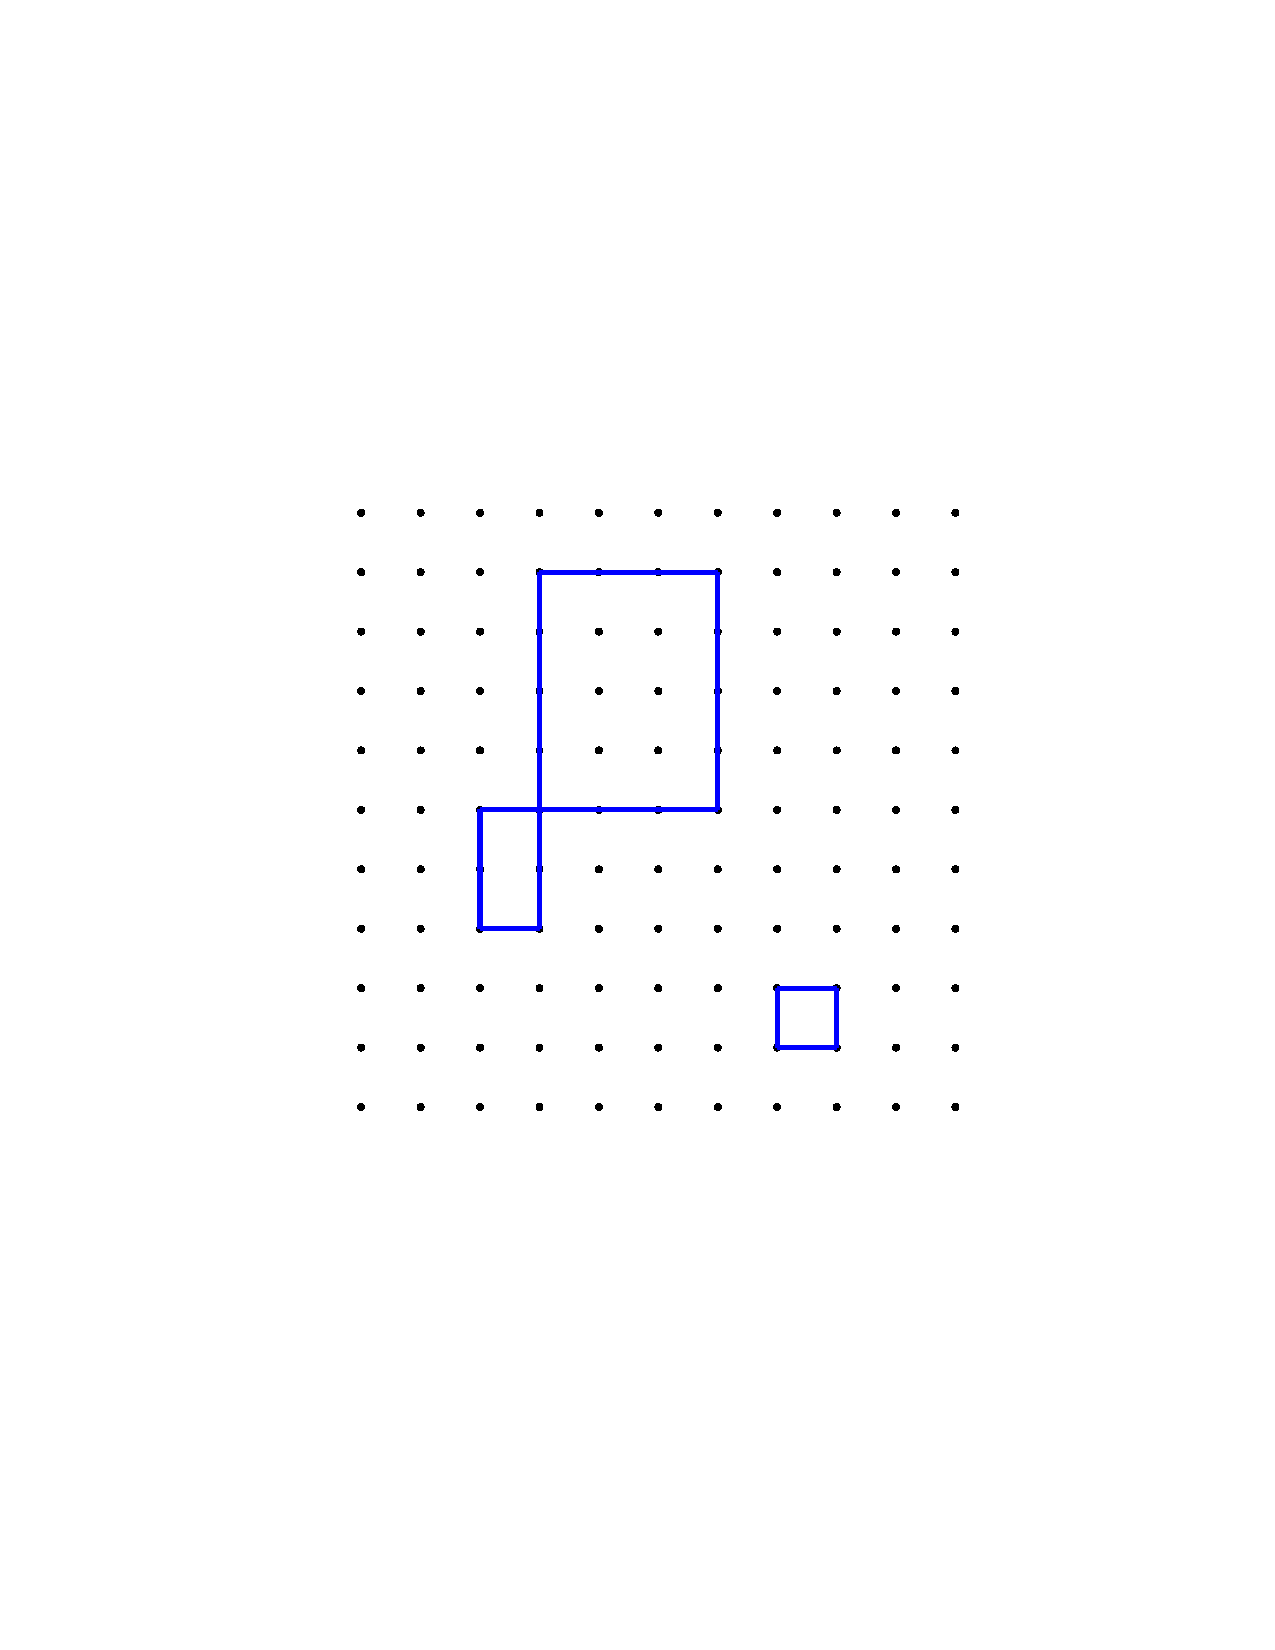
\includegraphics[width=0.49\textwidth]{graph_allowed}} 
\subfigure[Forbidden graph.]{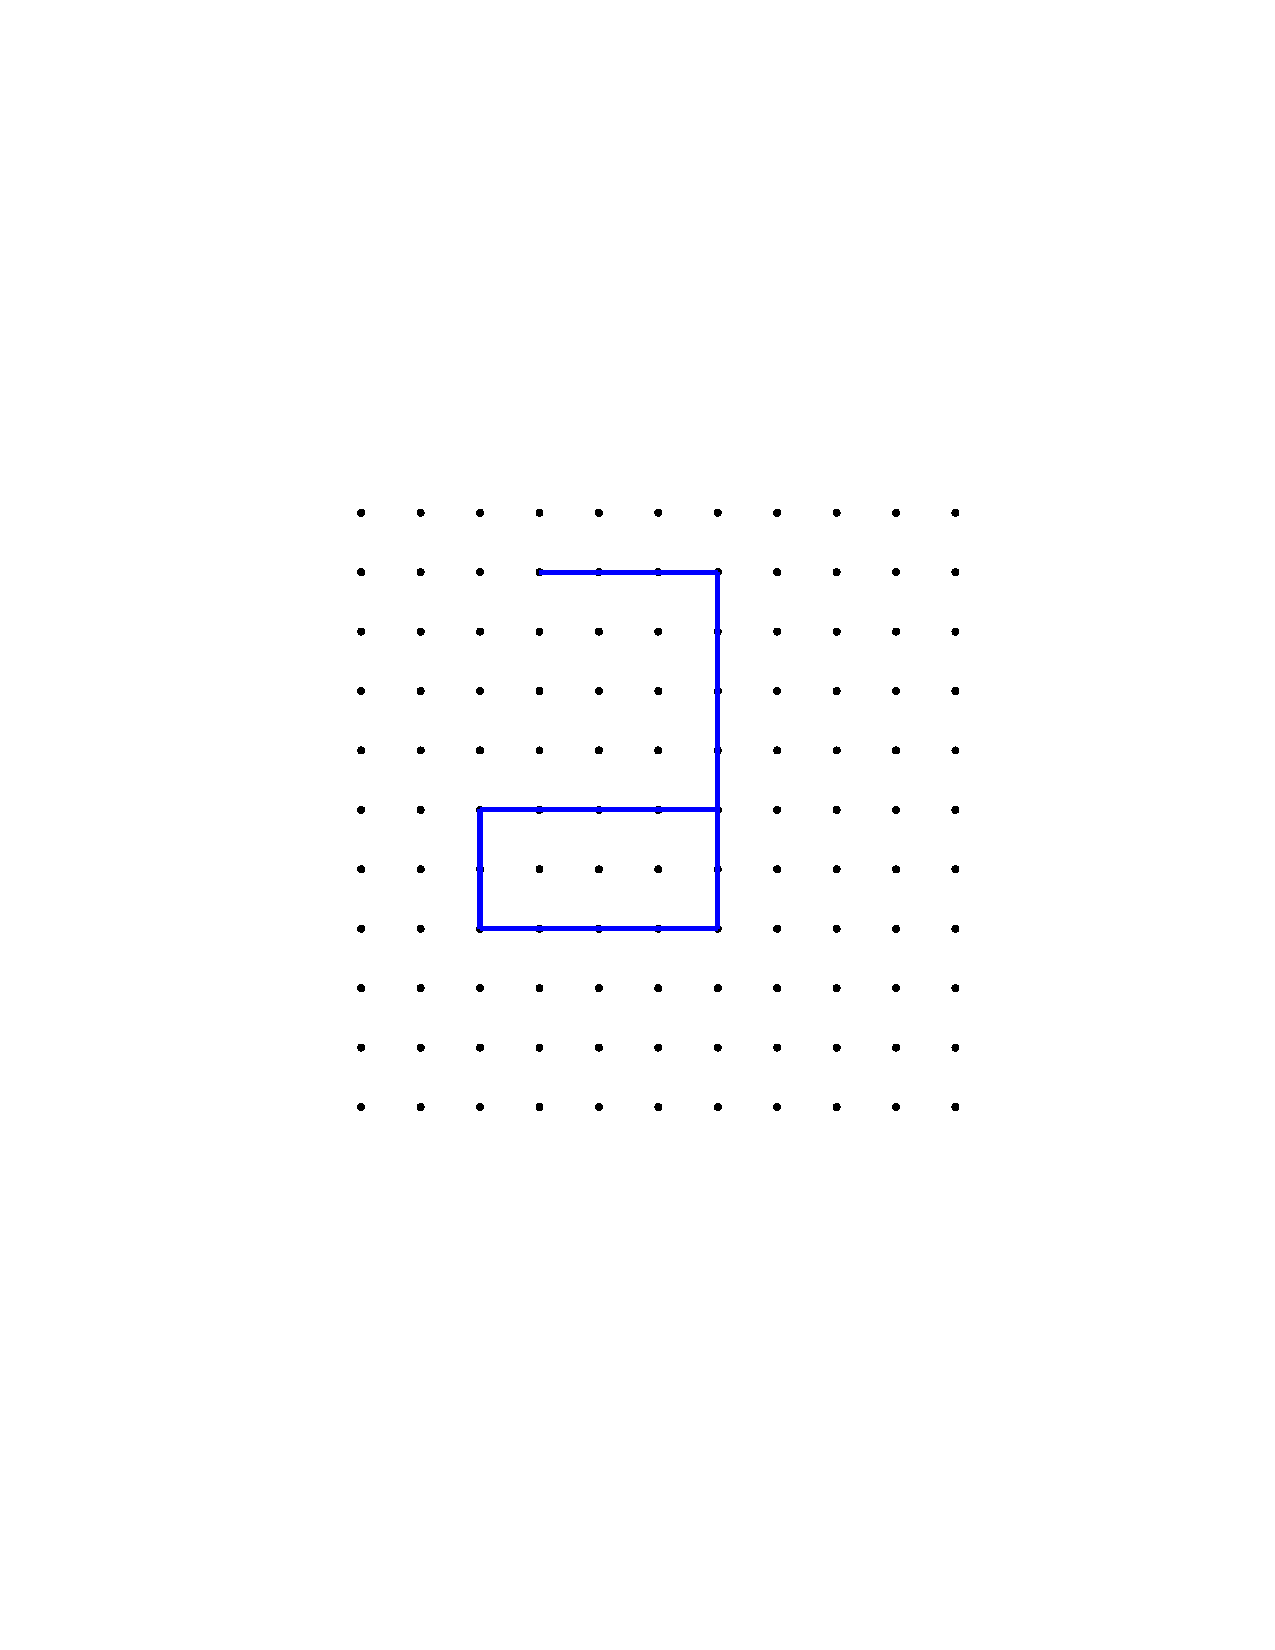
\includegraphics[width=0.49\textwidth]{graph_not_allowed}} 
\caption{{\it Graphical representation of the partition function of the Ising model.}\label{fig:graph:ising}}
\end{figure}
%
We can rewrite the sum over allowed graphs also in the form
\begin{align}\label{eq:ising:Z:g}
Z&=2^{N}\; \cosh^{2N}(j) \;\big(1+\sum_{n=4}^{\infty} g_{n}\;t^{n}\big)\;,
\end{align}
where $n$ is the number of edges and $g_{n}$ is the number of allowed graphs
with $n$ edges. We have already exploited that the smallest graph (besides the empty graph) has 4 edges.
Since each vertex has even order, the allowed graphs contain closed paths,
as can be seen in \fig{fig:graph:ising}. 



\subsection{Making the graphs unique}
The figure also contains a {\em node}, 
i.e. a vertex of order 4. Let's  try to draw the graph with a pencil on a piece of 
squared paper. We start at an arbitrary  vertex of order 2 and draw a line to one of the two connected vertices. If the next vertex also has order 2, it is obvious how to continue the drawing. When we reach a node, however, we have 3 options to continue:
{\it turn left, go straight, turn right}. 
It will turn out to be advantageous, to replace the graph by objects that allow to draw them in a unique way. Therefore, we will introduce graphical objects, that make a node unique. To this end a node is split into the three graphical objects, shown in
\fig{fig:ising:junction}.
%
\begin{figure}[h]
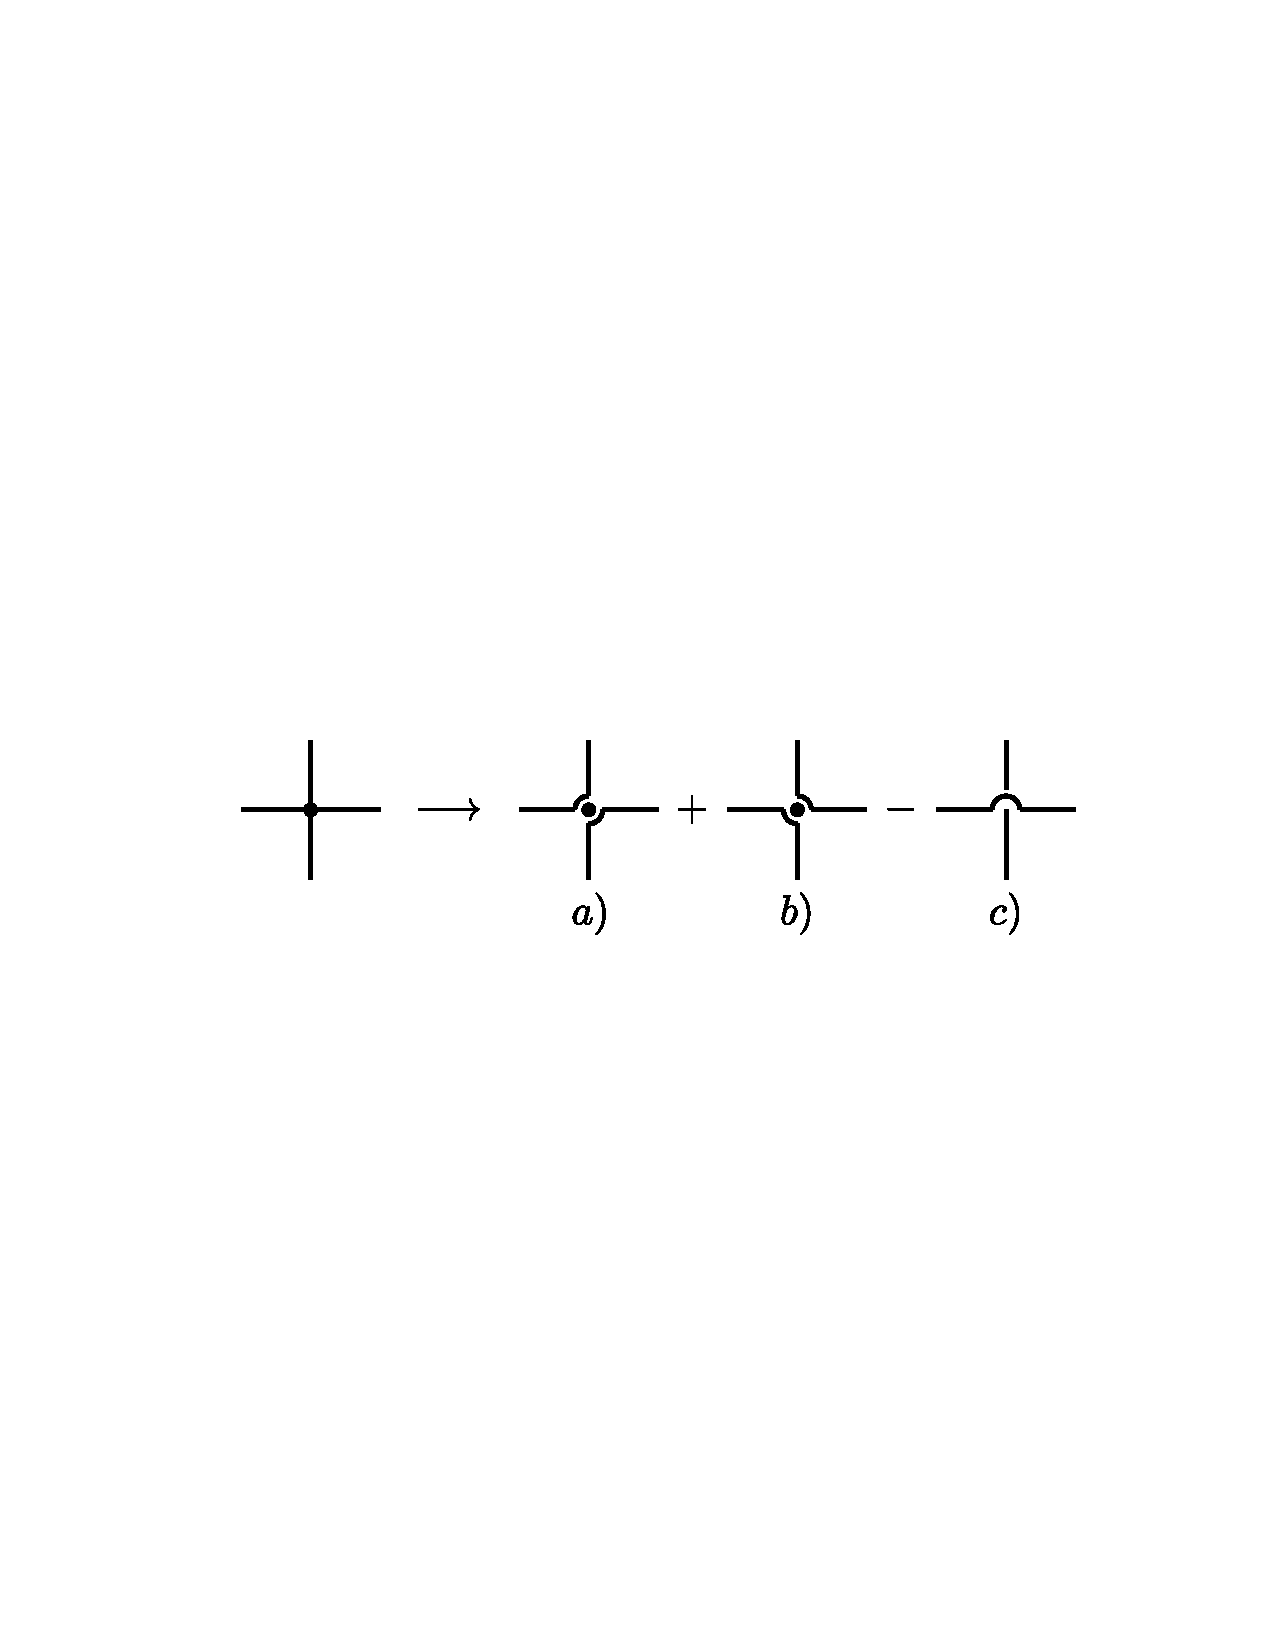
\includegraphics[width=1\textwidth]{junction}
\caption{{\it Splitting of a node with corresponding weights.}\label{fig:ising:junction}}
\end{figure}
%
This splitting  results in $3^{N_{n}}$
different new graphs, obtained from a graph with $N_{n}$ nodes. This would increase $g_{n}$ in a complicated way. To avoid this complication,
each new graphical element obtains a weight factor $\pm 1$, a shown in \fig{fig:ising:junction}. Now the three contributions of each node add up to $1$ again and the total count does not change.
The new graphs are denoted by $\tilde G$. They consist of one or more loops. 
As a remainder, a  {\em loop} (with e.g. $n$ edges) is a simply connected set  of edges, i.e. an object that can be drawn by starting at an arbitrary vortex on the loop, following the edges, and returning at the starting point after $n$ steps. The shortest loop has $4$ edges and the number of edges is always even.
In the new graphs $\tilde G$, the number of edges has not changed,   as compared to the  original graph,  but it has an extra weight factor
%
\begin{align*}
w(\tilde G) &= \big( -1 \big)^{N_{c}(\tilde G)}\;,
\end{align*}
%
where $N_{c}(\tilde G)$ stands for the number of \blue{crossings} ( decomposition c in \fig{fig:ising:junction}) of a graph $\tilde G$ of the new type.
By now $g_{n}$ is 
%
\begin{align*}
g_{n} &= \sum_{\tilde G}^{N_{e}(\tilde G)=n} \big( -1 \big)^{N_{c}(\tilde G)}\;.
\end{align*}
%

\subsection{Decomposing graphs into loops}
%
We are still not able to calculate the sum of all graphs analytically.
To this end we need to transform the graphs further.
Each graph $\tilde G$ with $n$ edges consists of  one or more loops,
which in total have $n$ edges. If a particular graph $\tilde G$ consists of $l$ loops,
we can devide the total weight between the loops. A loop $L$ contributes
a factor
%
$(-1)^{N_{c}(L)}\;$,
%
where $N_{c}(L)$ is the number of crossings in loop $L$.
The total weight is the product of the weights of the loops of  which the graph is formed.
Clearly, there is a one-to-one correspondence between all graphs $\tilde G$
with $n$ edges and all sets of loops with a total number $n$ of edges.
We define 
%
\begin{align}\label{eq:ising:def:D}
D_{l} &=
\begin{cases}
 \sum_{L}^{\text{loops with $l$ edges}}  \big( -1 \big)^{N_{c}(L)}&\text{if $l$ is even}	\\
 0&\text{otherwise}
\end{cases}\;.
\end{align}
%

Hence for $n\ge 4$ we may think that we can decompose $g_{n}$ into the contribution
of the loop decomposition:
%
\begin{align}\label{eq:ising:g:D}
g_{n}=\sum_{\tilde G} \delta_{N_{n}(\tilde G)=n} \;\big( -1 \big)^{N_{c}(\tilde G)}
&= \sum_{m=1}^{\infty} \frac{1}{m!} \sum_{l_{1}\ldots l_{m}=4}
\delta_{\sum_{\nu=1}^{m}l_{\nu} = n}
\prod_{\nu=1}^{m}
  D_{l_{\nu}}
\end{align}
%
Here $m$ is the number of loops and $l_{\nu}$ stands for the number of edges of loop $\nu$ and $D_{l_{v}}$ is the  corresponding weight obtained by summing over all realizations of a loop with $l_{\nu}$ edges. 
The factor $1/m!$ is required as the right hand sight creates a particulcar set of $m$
loops in $m!$ different permutations.
We can insert \eq{eq:ising:g:D} in \eq{eq:ising:Z:g} and obtain
%
\begin{align*}
\sum_{n=4}^{\infty} g_{n} t^{n}&=
\sum_{m=1}^{\infty} \frac{1}{m!} \sum_{l_{1}\ldots l_{m}=4}
 \underbrace{\sum_{n=4}^{\infty}
 \delta_{\sum_{\nu=1}^{m}l_{\nu} = n }
}_{\color{blue} = 1}
\prod_{\nu=1}^{m}
  D_{l_{\nu}} t^{l_{\nu}}\\
  &=
\sum_{m=1}^{\infty} \frac{1}{m!} 
\prod_{\nu=1}^{m}
\bigg(\sum_{l=4}  D_{l} t^{l}\bigg)\\
  &=
\sum_{m=1}^{\infty} \frac{1}{m!} 
\bigg(\sum_{l=4}  D_{l} t^{l}\bigg)^{m}\\
&=\exp\bigg( \sum_{l=4}  D_{l} t^{l} \bigg)-1
\end{align*}
%
Hence according to \eq{eq:ising:Z:g} we have
%
\begin{align}\label{eq:ising:ln:Z}
\ln(Z) &= N \ln(2) + 2N \ln\big(\cosh(j)\big) + \sum_{m=1}^{\infty}  D_{m} t^{m} \;.
\end{align}
%
%
\begin{figure}[t]
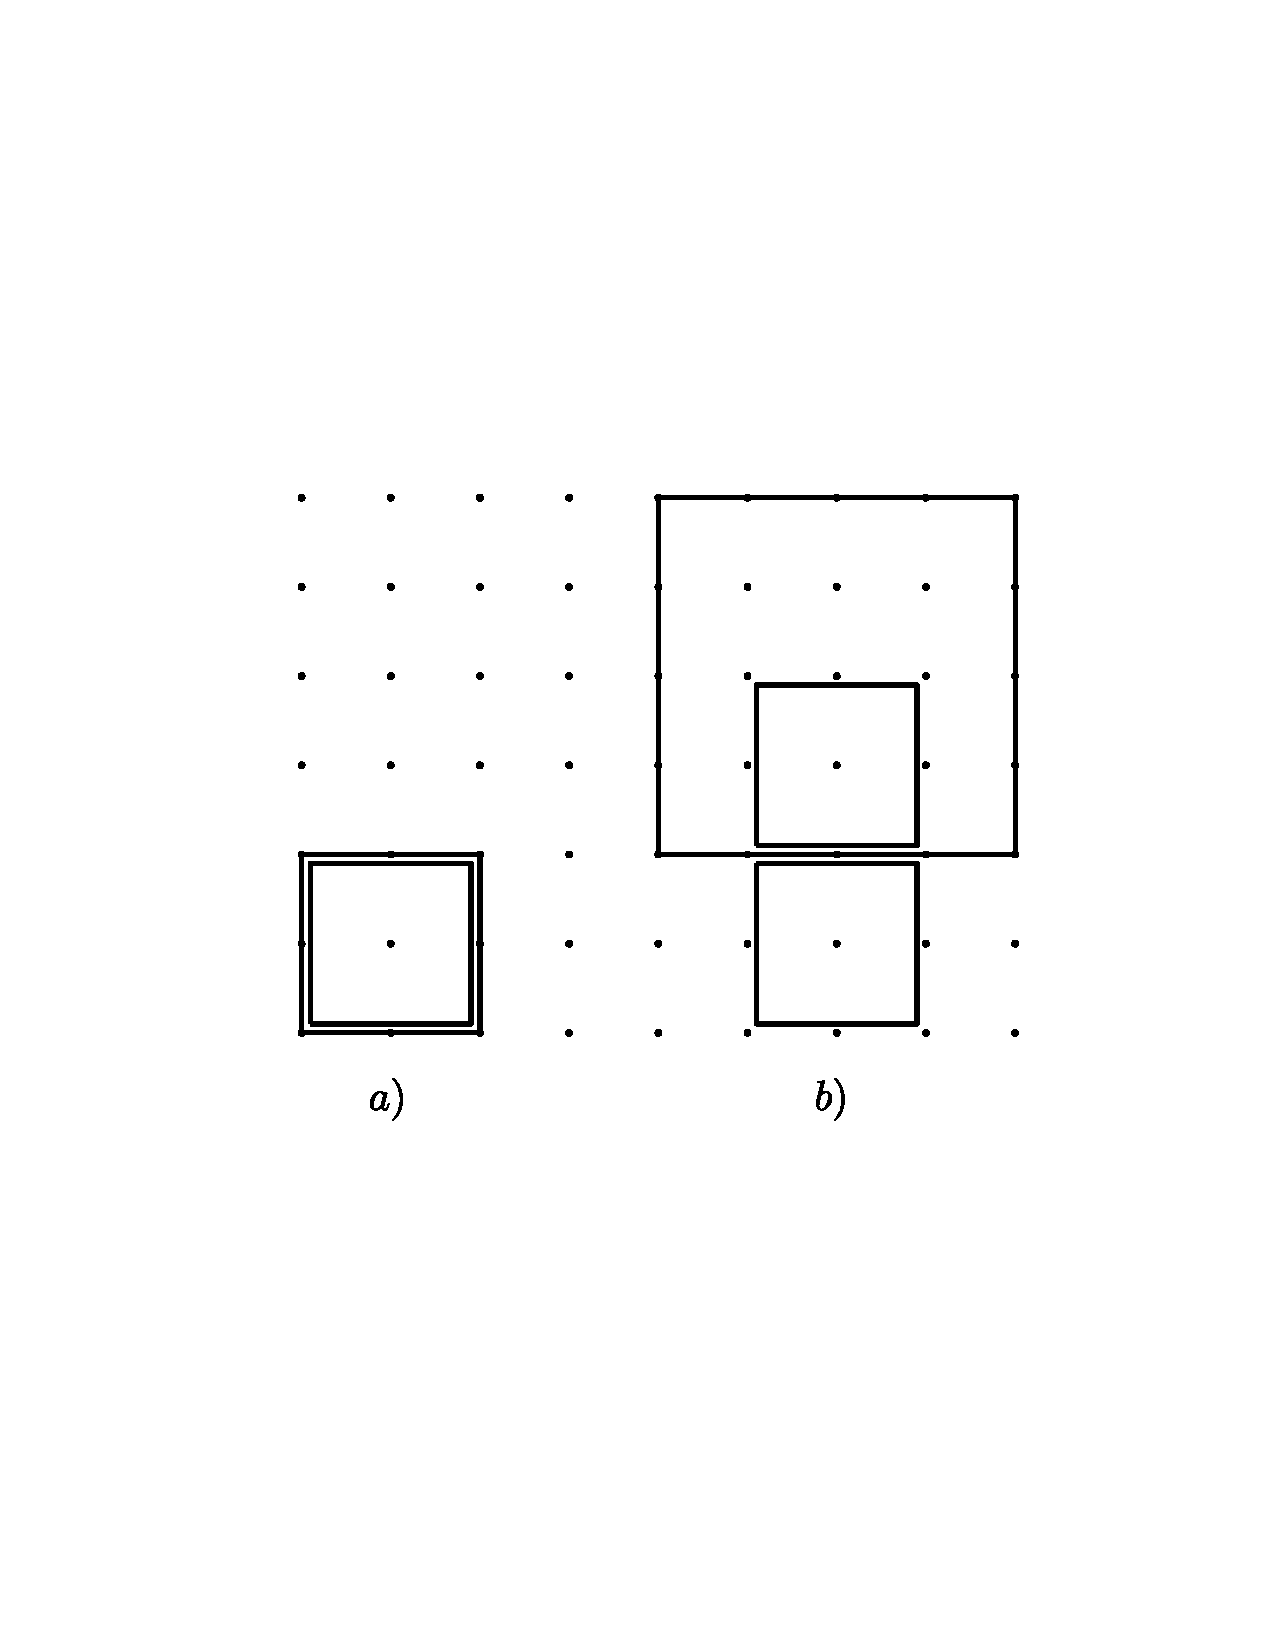
\includegraphics[width=.8\textwidth]{ising_crossings}
\caption{{\it Examples of configurations that occur if loops are placed independently. Such configurations are no valid graphs $\tilde G$.}\label{fig:ising:crossings}}
\end{figure}
%
The sum can start at $m=1$ (instead of $m=4$) since \eq{eq:ising:def:D} counts loops and the shortest loop has length $4$ anyways.
However, \eq{eq:ising:g:D} is not really correct. On the rhs the sum runs over all configurations
of independently arranged loops. I.e. there will be configurations where edges occur more than once, like in \fig{fig:ising:crossings}. Such a configuration is not included in $\tilde G$.
%
\begin{figure}[t]
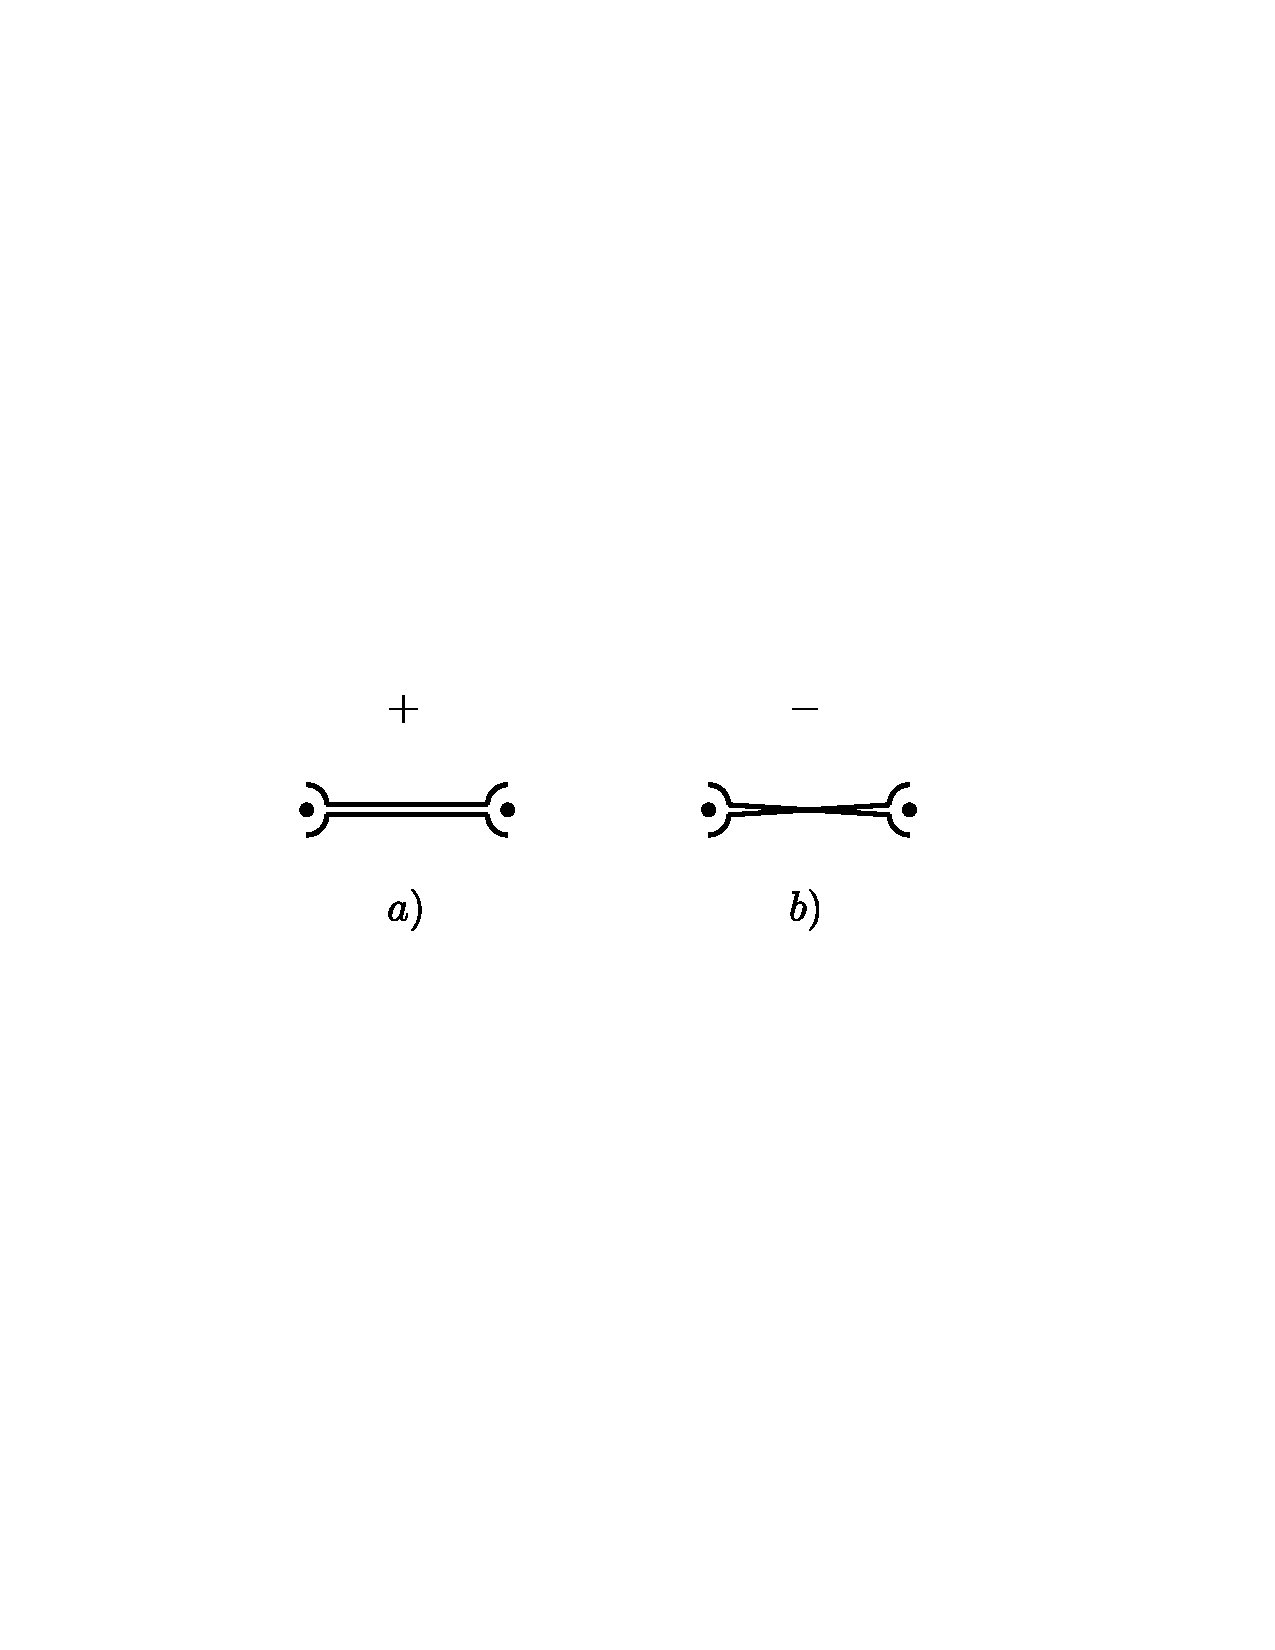
\includegraphics[width=.8\textwidth]{double_bonds}
\caption{{\it Double occupied edges.}\label{fig:ising:double:bonds}}
\end{figure}
%
However, there is a very simple cure. We allow such configurations also in $\tilde G$, but in addition to double bonds, say, as in  \fig{fig:ising:crossings} a) or schematically depicted in \fig{fig:ising:double:bonds} a)
we also include configurations that occur if we cross the lines as shown  in \fig{fig:ising:double:bonds} b) and give them a weight $-1$. 
The sum of these configurations adds up to zero.
The same holds true, if there are threefold
edges as in \fig{fig:ising:crossings} b) or even $m$-fold edges. Generally, in the case of $m$-fold edges there are $m!$ possible connections (permutations) of the incoming and outgoing lines. The number of crossings is even/odd  if the permutation is even/odd. As the number of even permutations is always equal to the number of odd permutations, the signs add up to zero.
In the case of \fig{fig:ising:crossings} a) the new configurations are depicted in
\fig{fig:ising:crossings:new}.
%
\begin{figure}[t]
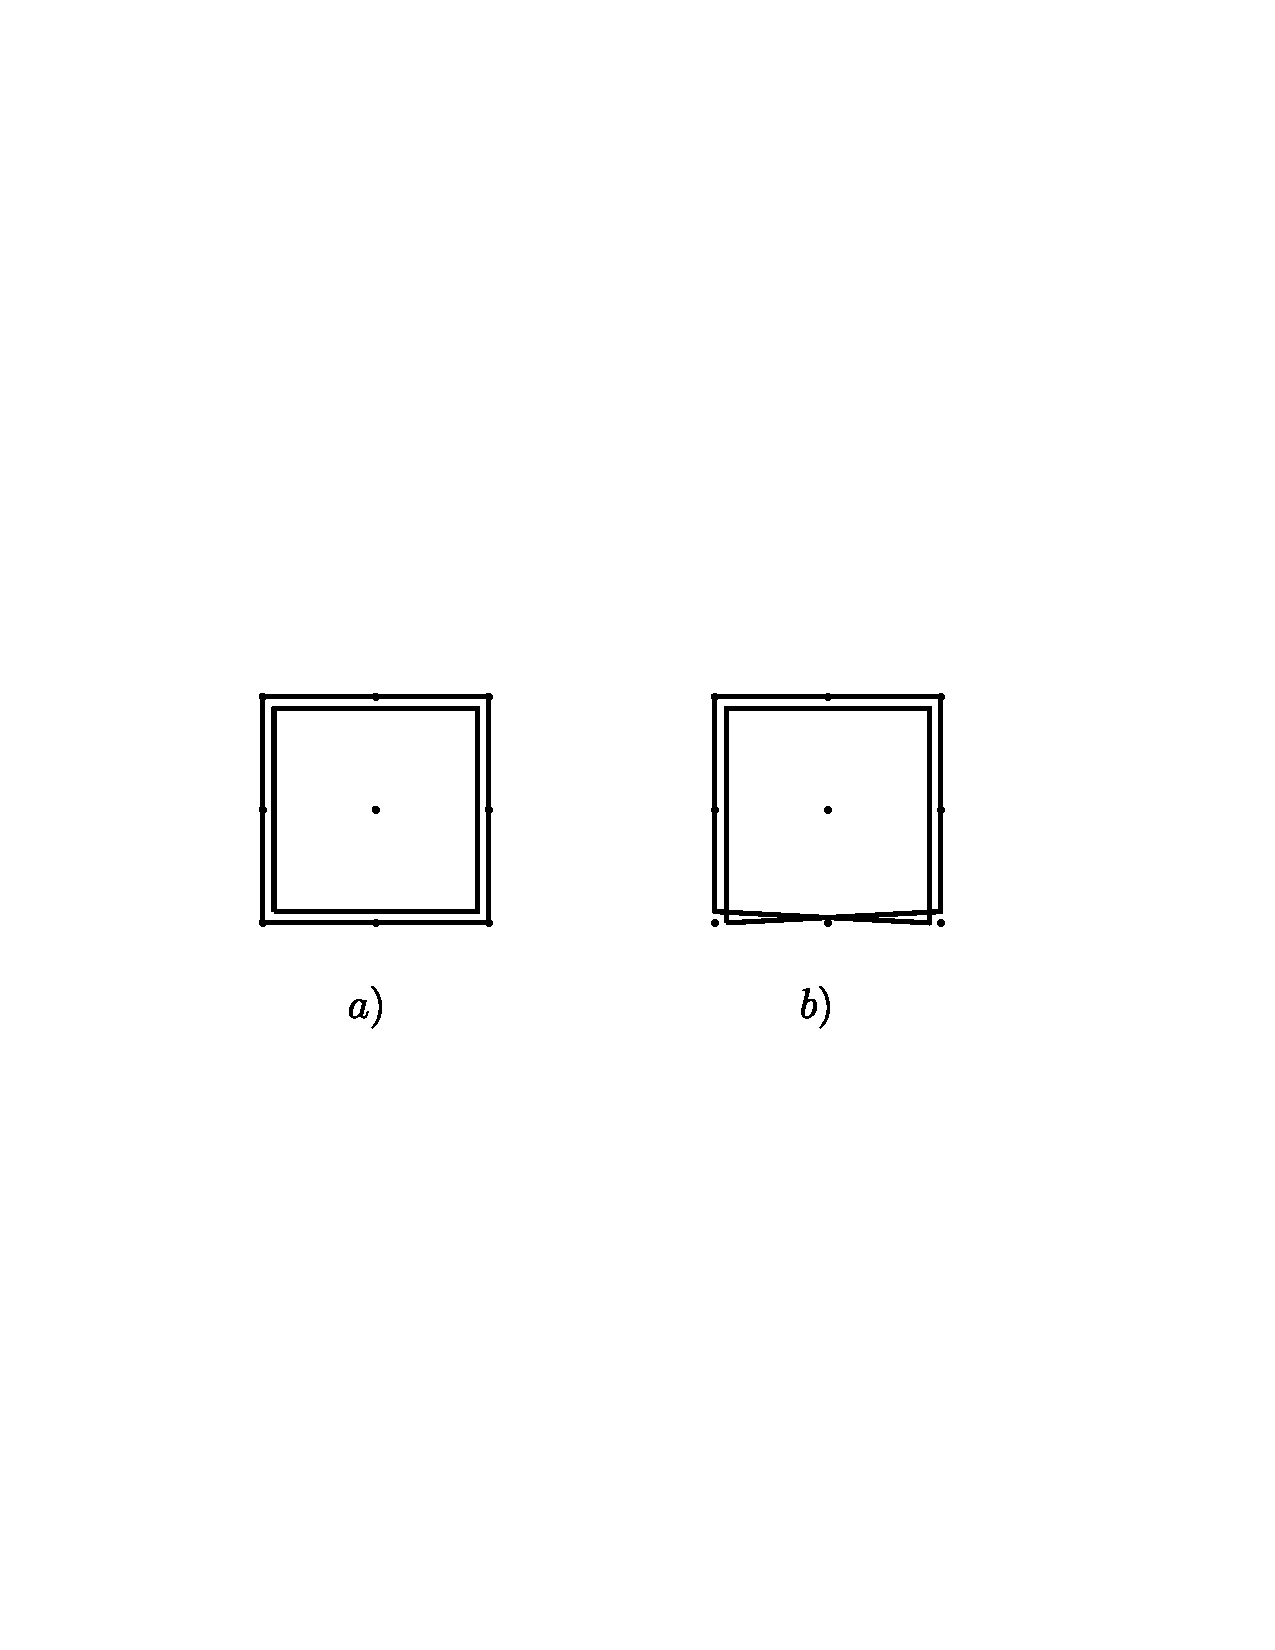
\includegraphics[width=.8\textwidth]{ising_crossings_new}
\caption{{\it Double occupied edges.}\label{fig:ising:crossings:new}}
\end{figure}
%
Now a) represents a double loop generated by placing loops independently, while b)
shows a single loop, which is passed twice. Including b) in the allowed single loops
ensures the cancelation of forbidden configurations generated by placing loops independently.
The same holds true for even more complex structures, such as tripple loops.

If we include the new type of crossings in the loops, then the previous formulas
 (\eq{eq:ising:def:D} and \eq{eq:ising:ln:Z})  remain unchanged, with the exception that these crossings also contribute to the number of crossings.
 
 

 \subsubsection{Counting then number of loops and corresponding crossing}
The remaining task is the determination of $D_{l}$, which includes the task of counting the crossings. To this end we introduce directed paths. The n-th step of the path is encoded in
%
\begin{align}
S^{(n)} &=\big( \vv x^{(n)}, \vv d ^{(n)}\big)\,
\end{align}
%
where $\vv x^{(n)}$ represents the initial site of the n-th step, 
and $\vv d^{(n)}\in\{\pm\vv e_{x},\pm\vv e_{y}\}$ 
the direction of the n-th step.  
A {\em path} from $S^{(0)}$ to $S^{(m)}$ is defined by the sequence
%
\begin{align*}
{\cal P}&=S^{(0)},S^{(1)},\ldots,S^{(m)}
\end{align*}
%
Clearly, we have the condition
%
\begin{align}\label{eq:ising:path:cond}
\vv x^{(n+1)} &=\vv x^{(n)} + \vv d^{(n)}\;.
\end{align}
%
As the allowed loops do not contain elements that occur when $\vv d^{(n+1)}=-\vv d^{(n)}$,
we omit such steps. We define the weight of such a path as
%
\begin{align}
w ({\cal P}) &= \prod_{l=1}^{m}e^{i \tfrac{1}{2}\Phi(\vv d^{(l-1)},\vv d^{(l)})}\;,
\end{align}
%
where $\Phi(\vv d, \vv d')$ is the angle between the vectors $\vv d$ and $\vv d'$, defined as follows.
%
\begin{align}\label{eq:}
\Phi(\vv d,\vv d') &=
\begin{cases}
	0&\text{if } \vv d , \vv d' \text{are parallel}\\
	\frac{\pi}{2}&\text{if } \vv d' \text{ is anti-clockwise rotated from } \vv d\\
		-\frac{\pi}{2}&\text{if } \vv d' \text{ is clockwise rotated from } \vv d\\
		\text{forbidden}&\text{if } \vv d , \vv d' \text{ are anti-parallel}
\end{cases}
\end{align}
%
\begin{figure}[t]
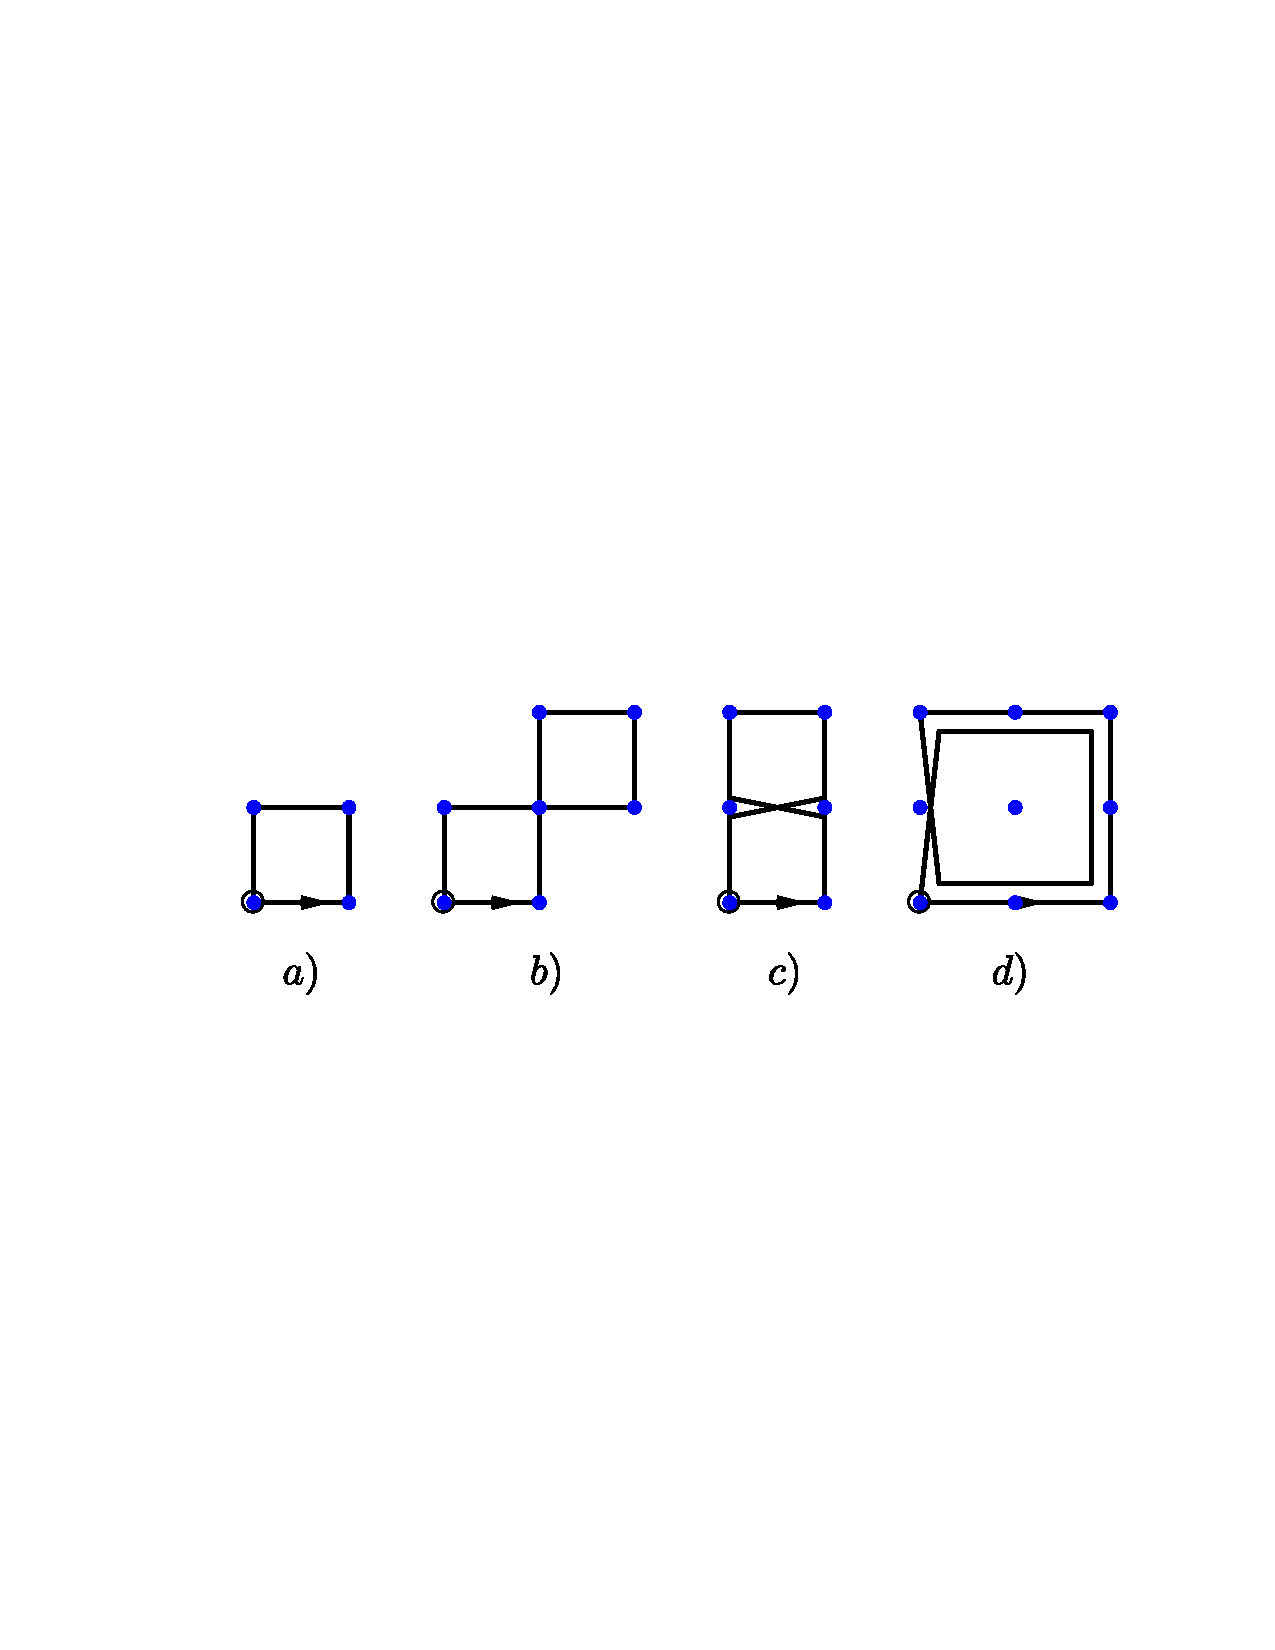
\includegraphics[width=.8\textwidth]{ising_paths}
\caption{{\it Representative paths and weights.}\label{fig:ising:paths}}
\end{figure}
%
In \fig{fig:ising:paths} some examples of allowed loops (paths) are given, for which we want to compute the weight. We start at the lower left corner and follow the arrow. 
We recall that turning left at a vertex gives $+\tfrac{\pi}{2}$, a right turn $-\tfrac{\pi}{2}$
and crossing straight adds zero.
In subfigure a)
the 4 angles $\Phi$ encountered during the path are all $\pi/2$. The four angle add up to $2 \pi$.
In other words we have performed four left turns
The weight is then
%
\begin{align*}
w &=e^{i \tfrac{1}{2} 2\pi} = -1\;.
\end{align*}
% 
For example b) the angles are in units of $\tfrac{\pi}{2}$: $1,0,-1,-1,-1,0,1,1$, with a sum of $0$ and a weight $w=+1$. In other words the number of left and right turns is equal. That is also the case in subfigure c). In example d) a loop is twice passed, so the total angle is $4 \pi$ and a phase factor $+1$.
We find in all  cases
%
\begin{align*}
w({\cal P}) &= - (-1)^{N_{c}(L)}\;,
\end{align*}
%
which is the required weight in \eq{eq:ising:def:D} apart from a global minus sign.

Now we define a matrix ${\cal M}$ with matrix elements
%
\begin{align*}
\bra{S'} M_{m}\ket{S} = \text{sum of the weights of all paths from $S$  to $S'$  in $m$ steps}\;.
\end{align*}
%
The value of the matrix element is zero, if there is no path connecting $S$ and $S'$
in $m$ steps.
For $m=m_{1}+m_{2}$  we have  by definition
%
\begin{align*}
\bra{S'} M_{m}\ket{S}  &=
\sum_{S''}\bra{S'} M_{m_{1}}\ket{S''} \bra{S''} M_{m_{2}}\ket{S}   \;,
\end{align*}
%
which is the common matrix product. Consequently, we have
%
\begin{align*}
{\cal M} _{m}  &= \big({\cal M}_{1}\big)^{m}\;.
\end{align*}
%
${\cal M}_{1}$ has the dimension $4 N\times 4N$, as each step $S=(\vv x,\vv d)$ has
$N$ possible sites $\vv x$ and 4 possible directions $\vv d$. Most of the matrix elements, however, are zero. The fact that a path cannot be retraced is also accounted for in ${\cal M}_{1}$.

We can now easily express the sought-for weight  $D_{m}$ as
%
\begin{align*}
D_{m} &= - \frac{1}{2m}\sum_{S} \bra{S} {\cal M}_{m} \ket{S}
= -\frac{1}{2m} \tr{{\cal M}_{1}^{m} }
\end{align*}
%
\emphasize{prove}{
\begin{enumerate}
	\item The trace is required to sum over all initial vertices of the loop and to make sure that the loop is really closed
	\item Since each vertex of a loop occurs as initial point in the trace, we have to divide by $m$
	\item Each loop can be traversed in two direction, which explains the factor $1/2$.
	\item The minus sign has been expained before.
\end{enumerate}
}
In total we therefore have according to \eq{eq:ising:ln:Z}
\begin{align*}
\ln(Z) &= N \ln(2) +2 N \ln\big(\cosh(j)\big) + \sum_{m=1}  D_{m} t^{m} \\
&= N \ln(2) + 2 N \ln\big(\cosh(j)\big)  - \frac{1}{2}\tr{\sum_{m=1} \frac{\big(t{\cal M}_{1}\big)^{m}}{m} }\\
&= N \ln(2) + 2 N \ln\big(\cosh(j)\big)  + \frac{1}{2}\tr{\ln\big(\mathbf 1-t{\cal M}_{1}\big)}\\
&= N \ln(2) + 2 N \ln\big(\cosh(j)\big)  + \frac{1}{2}\ln\text{det}\big[\big(\mathbf 1-t{\cal M}_{1}\big)\big]\;.
\end{align*}

As said before, the size of the matrix ${\cal M}_{1}$ is $4N\times 4N$. The matrix elements are defined via
%
\begin{align*}
\bra{\vv  x,\vv d} {\cal M}_{1}\ket{\vv x',\vv d'}\;.
\end{align*}
%
Since we use pbc, it is advantageous to perform a Fourier transform with respect to $\vv x$ and 
$\vv x'$. The determinant is invariant against such a unitary transformation. Moreover, due to
translational invariance of the problem, we obtain
%
\begin{align*}
\bra{\vv  q,\vv d} {\cal M}_{1}\ket{\vv q',\vv d'}&=
\frac{1}{N}\sum_{\vv x,\vv x'} e^{-i\big(\vv x\cdot \vv q-\vv x'\cdot \vv q'\big)}
\bra{\vv 0,\vv d} {\cal M}_{1}\ket{\underbrace{\vv x'-\vv x}_{\Delta\vv  x},\vv d'}\\
&= \underbrace{
\frac{1}{N}\sum_{\vv x} e^{-i\vv x\cdot (\vv q-\vv q')}
}_{\color{blue} = \delta_{\vv q\vv q'}}\sum_{\Delta\vv x} e^{i \vv q'\cdot\Delta \vv x}
\bra{\vv 0,\vv d} {\cal M}_{1}\ket{\Delta\vv  x,\vv d'}\\
&= \delta_{\vv q\vv q'}\;\sum_{\Delta\vv x} e^{i \vv q\cdot\Delta \vv x}
\bra{\vv 0,\vv d} {\cal M}_{1}\ket{\Delta\vv  x,\vv d'}\;.
\end{align*}
%
According to \eq{eq:ising:path:cond} we have the condition 
%
\begin{align*}
\vv x' &= \vv x +\vv d\\
\Rightarrow\qquad \Delta \vv x &= \vv x' -\vv x = \vv d\;.
\end{align*}
%
Hence the $4\times 4$ matrix $M(\vv q)$ hat the matrix elements
%
\begin{align*}
\bra{\vv  q,\vv d} {\cal M}_{1}\ket{\vv q',\vv d'}
&= \delta_{\vv q\vv q'}\; 
e^{i \vv q\cdot\vv d}\;
\bra{\vv 0,\vv d} {\cal M}_{1}\ket{\vv d,\vv d'}\\
&= \delta_{\vv q\vv q'}\; 
\underbrace{
e^{i \vv q\cdot\vv d}\;
e^{i\frac{1}{2}\Phi(\vv d,\vv d')}
}_{\color{blue} = M_{\vv d,\vv d'}}\\
\end{align*}
%
The inverse transformation is
%
\begin{align*}
\bra{\vv  x,\vv d} {\cal M}_{1}\ket{\vv x',\vv d'}&=\frac{1}{N}
\sum_{\vv q} e^{i\big(\vv x-\vv x')\cdot \vv q }
\bra{\vv q,\vv d} {\cal M}_{1} \ket{\vv q,\vv d'}\;,
\end{align*}
%
and, therefore, 
%
\begin{align*}
\bra{\vv  x,\vv d} {\cal M}^{n}\ket{\vv x',\vv d'}&=\frac{1}{N}
\sum_{\vv q} e^{i\big(\vv x-\vv x')\cdot \vv q }
\bra{\vv q,\vv d} ({\cal M}_{1})^{n} \ket{\vv q,\vv d'}\\
&=\frac{1}{N}
\sum_{\vv q} e^{i\big(\vv x-\vv x')\cdot \vv q }
\bigg(\big( M(\vv q) \big)^{n}\bigg)_{\vv d,\vv d'}\;.
\end{align*}
%

The remaining  $4\times 4$ matrix $M(\vv q)$ has the matrix elements
%
%
%\begin{center}
%M:
% \begin{tabular}{||c|c c c c||} 
% \hline
% $\vv d \backslash  \vv d' $&$\vv e_{x}$ & $\vv e_{y}$ & $-\vv e_{x}$  &$-\vv e_{y}$ \\ [0.5ex] 
% \hline\hline
%$\vv e_{x}$  &$e^{iq_{1}}$& $\lambda e^{i q_{1}}$& $0$ & $\lambda^{*}e^{iq_{1}}$ \\ 
% \hline
% $\vv e_{y}$&$\lambda^{*} e^{i q_{2}}$& $e^{iq_{2}}$ & $\lambda e^{i q_{2}}$  & $0$ \\
% \hline
%$-\vv e_{x}$ &$0$ & $\lambda^{*} e^{-i q_{1}}$& $e^{-iq_{1}}$  & $\lambda e^{-i q_{1}}$ \\
% \hline
%$-\vv e_{y}$ &$\lambda e^{-i q_{2}}$& $0$  &$\lambda^{*} e^{-i q_{2}}$ & $e^{-iq_{2}}$ \\[1ex] 
% \hline
%\end{tabular}
%\end{center}
%
\begin{center}
$M(\vv  q)$:
 \begin{tabular}{||c|c c c c||} 
 \hline
 $\vv d \backslash  \vv d' $&$\vv e_{x}$ & $-\vv e_{x}$ & $\vv e_{y}$  &$-\vv e_{y}$ \\ [0.5ex] 
 \hline\hline
$\vv e_{x}$  &$e^{iq_{1}}$& $0$& $\lambda e^{i q_{1}}$ & $\lambda^{*}e^{iq_{1}}$ \\ 
\hline
$-\vv e_{x}$ &$0$ & $e^{-iq_{1}}$& $\lambda^{*} e^{-i q_{1}}$  & $\lambda e^{-i q_{1}}$ \\
 \hline
 $\vv e_{y}$&$\lambda^{*} e^{i q_{2}}$& $\lambda e^{i q_{2}}$ & $e^{iq_{2}}$  & $0$ \\
 \hline
$-\vv e_{y}$ &$\lambda e^{-i q_{2}}$  &$\lambda^{*} e^{-i q_{2}}$& $0$ & $e^{-iq_{2}}$ \\[1ex] 
 \hline
\end{tabular}
\end{center}
%

with the definition $\lambda=e^{i\tfrac{\pi}{4}}$.
This can also be written as
%
\begin{subequations}\label{eq:}
\begin{align}
M(\vv q) &=  D(\vv q) \tilde M\\
D(\vv q) &=\text{diag} \big[ e^{i q_{1}},e^{-i q_{1}},e^{i q_{2}} ,e^{-i q_{2}}\big]\\
\tilde M &=
\begin{pmatrix}
	1&0&\lambda,\lambda^{*}\\
		0&1&\lambda^{*},\lambda\\
\lambda^{*},\lambda&	1&0&\\
\lambda,\lambda^{*}&	0&1&
\end{pmatrix}
\end{align}
\end{subequations}
%
Here $\tilde M$ is a hermitean matrix bat $M$ is not.
As the matrix is blockdiagonal in $\vv q$, $\vv q'$ we have
%
\begin{align*}
\text{det} \big(\mathbf 1- t {\cal M}_{1} \big)=\text{det} \big(t {\cal M}_{1} - \mathbf 1 \big)
&=\prod_{\vv q}^{1bc} \det\big( t M(\vv q)  - \mathbf 1 \big)
\end{align*}
%
With $Q_{\alpha}=t e^{iq_{\alpha}}$ the matrix  argument of the determinant reads
%
%\begin{align*}
%  t M(\vv q) - \mathbf 1=
%\begin{pmatrix}
%Q_{1}-1& \lambda Q_{1}&0& \lambda^{*} Q_{1}\\
% \lambda^{*}Q_{2}&Q_{2}-1& \lambda Q_{2}&0\\
%0& \lambda^{*}Q_{1}^{*}&Q_{1}^{*}-1& \lambda Q_{1}^{*}\\
% \lambda Q_{2}^{*}&0& \lambda^{*}Q_{2}^{*}&  Q_{2}^{*}-1
%\end{pmatrix}
%\end{align*}
%%


%
\begin{align*}
  t M(\vv q) - \mathbf 1=
- \begin{pmatrix}
Q_{1}-1& 0& \lambda Q_{1}& \lambda^{*} Q_{1}\\
0& Q_{1}^{*}-1&\lambda^{*}Q_{1}^{*}& \lambda Q_{1}^{*}\\
\lambda^{*}Q_{2}&\lambda Q_{2}&Q_{2}-1& 0\\
 \lambda Q_{2}^{*}& \lambda^{*}Q_{2}^{*}& 0& Q_{2}^{*}-1
\end{pmatrix}\;.
\end{align*}
%
The determinant  yields (according to MATHEMATICA)

%
\begin{align*}
\ln
\bigg[
\det \big(
\mathbf 1- t {\cal M}_{1} 
\big)\bigg] &=\sum_{\vv q}^{1bz}
\ln
\bigg[ 
\big( 1+t^{2} \big)^{2}
-2t (1-t^{2}) 
\big( \cos(q_{1})+\cos(q_{2})
\big) 
\bigg]\;.
\end{align*}
%
Then the free energy per site is 
%
\begin{align}\label{eq:}
-\beta\frac{F}{N} &= \ln(2) + 2\ln(\cosh(j)) +\frac{1}{2N}\sum_{\vv q}^{1bc}
\ln\bigg[ \big( 1+t^{2} \big)^{2}-2t (1-t^{2}) \big( \cos(q_{1})+\cos(q_{2}) \big) \bigg]
\end{align}
%
We introduce the normalized density of states $\rho(\varepsilon)$ corresponding to the dispersion
%
\begin{align}\label{eq:ising:dispersion}
 \varepsilon(\vv q) &= - \big( \cos(q_{1})+\cos(q_{2} ) \big) \\
 \rho(\varepsilon) &= \frac{1}{N}\sum_{\vv q}^{1bc} \delta(\varepsilon(\vv q) - \varepsilon)
\end{align}
%
Then the free  energies reads
%
\begin{align}\label{eq:}
-\beta\frac{F}{N} &= \ln(2) + 2\ln(\cosh(j)) +\frac{1}{2}\int d\varepsilon \rho(\varepsilon)
\ln\big[ \big( 1+t^{2} \big)^{2}+2t (1-t^{2}) \;\varepsilon \big]\;.
\end{align}
%
Moreover, we use
%
\begin{align*}
\cosh(j) &=\frac{1}{\sqrt{1-t^{2}}}\;,\qquad \big(t:=\tanh(j)\big)\\
2 \ln\big(  \cosh(j)\big) &= \frac{1}{2}\ln\big( (1-t^{2})^{-2} \big)
= \frac{1}{2} \int d\varepsilon\; \rho(\varepsilon)  \ln\big(\big( 1-t^{2} \big)^{-2}\big)
\end{align*}
%
to obtain
\begin{align*}
-\beta\frac{F}{N} &= \ln(2) +\frac{1}{2}\int d\varepsilon \rho(\varepsilon)
\ln\bigg[ \bigg( \frac{1+t^{2}}{1-t^{2}} \bigg)^{2}+ \bigg(\frac{2t}{1-t^{2}}\bigg) \;\varepsilon\bigg]\\
&= \ln(2) +\frac{1}{2}\int d\varepsilon \rho(\varepsilon)
\ln\bigg[\underbrace{
 \bigg( \frac{1+t^{2}}{1-t^{2}} \bigg)^{2}-  \bigg(\frac{4t}{1-t^{2}}\bigg)
}_{\color{blue} = \big( 1-\sinh(2j) \big)^{2}}+ \underbrace{
\bigg(\frac{2t}{1-t^{2}}\bigg)
}_{\color{blue} = \sinh(2j)} \;(2+\varepsilon) \bigg]\;.
\end{align*}
%
%
\emphasize{proof}{
%
\begin{align*}
\frac{2 t}{1-t^{2}} &=\frac{2 \tanh(j)}{1-\tanh^{2}(j)}\\
  &=\frac{2 sh/ch}{(\underbrace{
ch^{2}-sh^{2}
}_{\color{blue} = 1})/ch^{2}} \\
&=2 \sinh(j) \cosh(j) = \sinh(2j)\\
%%%%
 \bigg( \frac{1+t^{2}}{1-t^{2}} \bigg)^{2}-  \bigg(\frac{4t}{1-t^{2}}\bigg) &=
\bigg( \frac{\overbrace{
ch^{2}+sh^{2}
}^{\color{blue} = \cosh(2j)}}{\underbrace{
ch^{2}-sh^{2}
}_{\color{blue} = 1}}\bigg)^{2}-  \underbrace{
\bigg(2\frac{2t}{1-t^{2}}\bigg) 
}_{\color{blue} = 2 \sinh(2j)}
 \\
 &=\cosh^{2}(2j) - 2 \sinh(2j) \\
 &= 1 + \sinh^{2}(2j) - 2 \sinh(2j) \\
 &= \big( 1-\sinh(2j) \big)^{2}\;.
\end{align*}
%
}
The final result for the free energy reads thereore
\tboxitp{Free Energy of the 2d Ising Model}{without external field}{
\begin{align}\label{eq:ising:ln:Z}
\frac{\ln(Z)}{N}=-\beta\frac{F}{N} 
&= \ln(2) +\frac{1}{2}\int d\varepsilon \rho(\varepsilon)
\ln\bigg[\big( 1-\sinh(2j) \big)^{2}+\sinh(2j) \;(2+\varepsilon) \bigg]\;.
\end{align}}
%
%
It is to be remembered that $j =J\beta>0$ for the ferrromagnetic model. Therefore, $\sinh(2j)>0$.
According to \eq{eq:ising:dispersion}, the energies $\varepsilon$ are restricted to the interval $([-2,2]$.
The density of states $\rho(\varepsilon)$ is that of the 2d tight binding model, which is given by
%
\begin{align}
\rho(\varepsilon)  &= \frac{\theta\big( \abs{\varepsilon}\le 2 \big)}{2\pi^{2}}\;{\cal K}\bigg( 1-\big(\frac{\varepsilon}{2}\big)^{2} \bigg)\;,
\end{align}
%
where ${\cal K}(x)$ is the elliptic integral of the first kind
%
\begin{align}\label{eq:}
{\cal K}(x) = \int_0^{\frac{\pi}{2}} \frac {\mathrm d\varphi}{\sqrt{1 - x^2(\sin \varphi)^2}}\;.
\end{align}
%
%
\begin{figure}[t]
\begin{center}
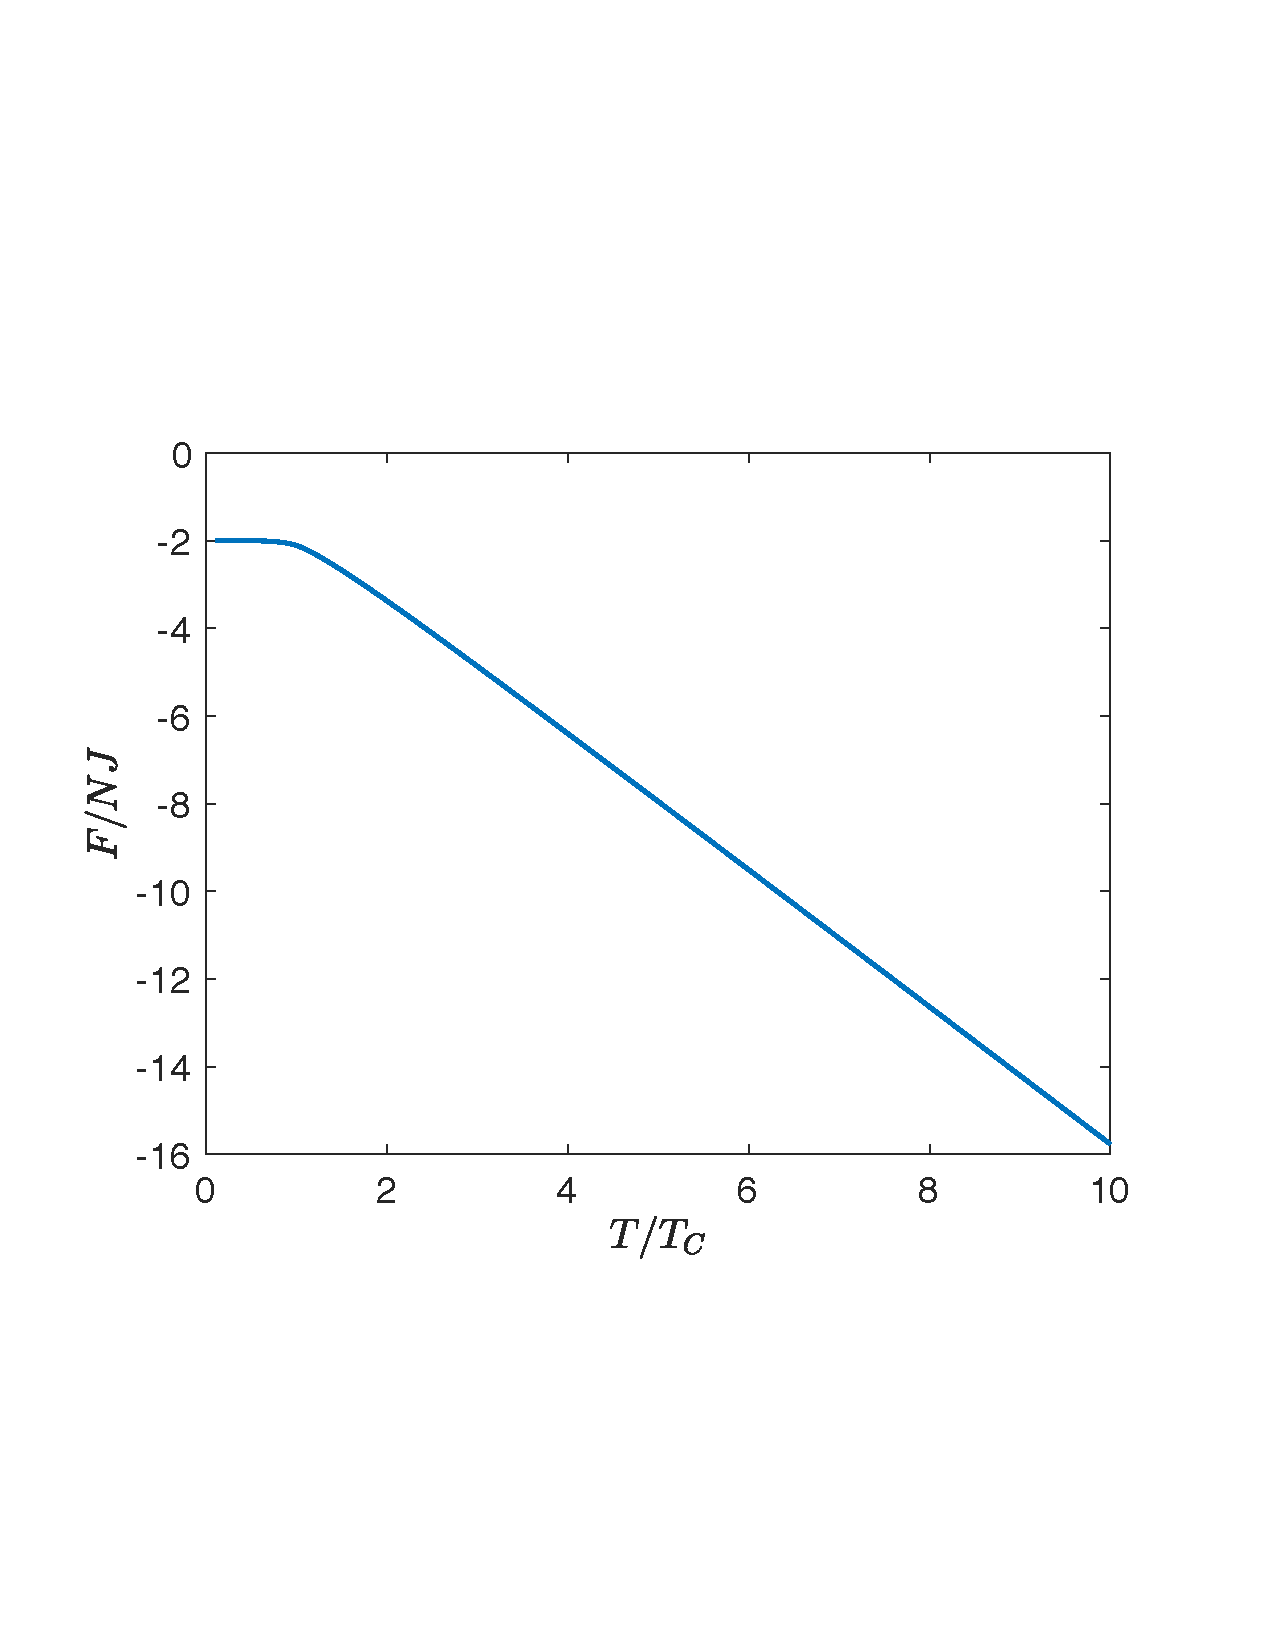
\includegraphics[width=10cm]{ising_free_energy}
\caption{{\it Free energy of the 2D Ising model.}}
\end{center}
\end{figure}
%
The free energy is related to the entropy and internal energy through
%
\begin{align*}
F &= U -T S\;.
\end{align*}
%
As we will easily see later on, for $T\to 0$ we have $U\to -2 J N$
and $S\to 0$  (3. law of thermodynamics), hence $F\to -2 J N$;
while for $k_{B}T/J \gg 1$ we have $U\to 0$
and $S\to N k_{B} \ln(2)$, hence $F\to - N k_{B} T \ln(2)$.

\subsection{Curie-temperature}

If we would have computed the free energy in the presence of an external magnetic field,
we could have computed the magnetization  and from that directly the transition temperature. 
In the absence of an external field, the magnetization is always zero, due to symmetry.
But in order to allow for a  phase transition the free energy has to have an irregularity.
(The argument will be given later.)
The argument of the logarithm is non-negative, but it can be zero which yields the required irregularity.
For the argument to become zero, both terms $(1-\sinh(2j))^{2}$ and $\sinh(2j)(2+\varepsilon)$ have to be zero.
The first condition yields
%
\begin{align}\label{eq:jC:2d:ising}
\sinh(2 j_{C}) &=1 
\end{align}
%
%
\begin{align*}
1 -\sinh(2j) &=  1 - \frac{e^{2j_{C}}+e^{-2j_{C}}}{2} = 0\\
\Rightarrow\qquad e^{2j_{C}}+e^{-2j_{C}} -2 &=0\\
e^{4j_{C}} -2 e^{2j_{C}} + 1&=0\;.
\end{align*}
%
This quadratic equation has the solutions
%
\begin{align*}
e^{2j_{C}} &= 1 \pm\sqrt{2}\;.
\end{align*}
%
Since $e^{2j}>0$ the only solution is 
%
\begin{align}\label{eq:}
j_{C} = J \beta_{C} &= \frac{1}{2}\ln\big( 1+\sqrt{2} \big) = 0.4407\;.
\end{align}
%
\blue{The mean field result was $J \beta_{C} = 0.25$.}
The irregularity  of the free energy is a necessary prerequisite for phase transition, but not 
sufficient for a rigorous prove. Nor does it tell us the order of the phase transition.
The rigorous prove requires the dependence of the free energy on the an external field.
\newpage

\subsection{Internal energy}
%
\begin{align*}
U &= \langle H \rangle = -J\sum_{\langle ij \rangle} \langle S_{i}S_{j}\rangle\;.
\end{align*}
%
Due to the translational invariance all n.n. correlations are
the same
\begin{align*}
\frac{U}{NJ} &=-2 \langle S_{1}S_{2}\rangle\;.
\end{align*}
For high temperatures the spins are uncorrelated resulting in
\begin{align*}
\frac{U}{NJ} &=-2 \langle S_{1}\rangle \langle  S_{2}\rangle = 0\;,
\end{align*}
while for $T=0$, the lowest energy is obtained if all spins are parallel 
and
\begin{align*}
\frac{U}{NJ} &=-2\;.
\end{align*}
Now we compute $U$ for arbitrary temperature.
%
To this end, we write $\ln(Z)$ in a more compact form
%
\begin{align*}
\ln(Z) &= \ln(2) +\frac{1}{2} 
\underbrace{
\avg{\ln \bigg((1-\kappa)^{2} + \kappa (2+\varepsilon) \bigg)}
}_{\color{blue} = g(\kappa)}\;,
\end{align*}
%
the average here is taken w.r.t. $\rho(\varepsilon)$, and $\kappa=\sinh(2 \beta J)$. Then
\begin{align*}
\frac{U}{N} &= \frac{\langle H \rangle}{N} = -\frac{\partial \ln(Z)}{\partial \beta}\\
&=-\frac{1}{2} \big(\frac{\partial }{\partial \kappa} g(\kappa) \big)
\frac{d \kappa}{d\beta}\;.
\end{align*}
%
with
%
\begin{align*}
\frac{\partial \kappa}{\partial \beta}&= \frac{\partial }{\partial \beta} \sinh(2 J \beta) = 2 J \cosh(2 J \beta)= 2J \sqrt{ 1+\sinh^{2}(2 J\beta) }
\end{align*}
%
we have 
%
\begin{align*}
\frac{U}{N}&=-J g'(\kappa) 
\sqrt{1+\kappa^{2}} \\
&=-J \avg{
\frac{2\kappa +\varepsilon}{(1-\kappa)^{2}+\kappa(2+\varepsilon)}
}
\sqrt{1+\kappa^{2}} \;.
\end{align*}
%
In summary we have
%
\tboxit{Internal energy}{
\begin{align}\label{eq:ising:U}
\frac{U}{N J} &= -  \avg{
\frac{2\kappa +\varepsilon}{(1-\kappa)^{2}+\kappa(2+\varepsilon)}
}
\sqrt{1+\kappa^{2}} \;.
\end{align}}
%

%
\begin{figure}[t]
\subfigure[Internal energy .]{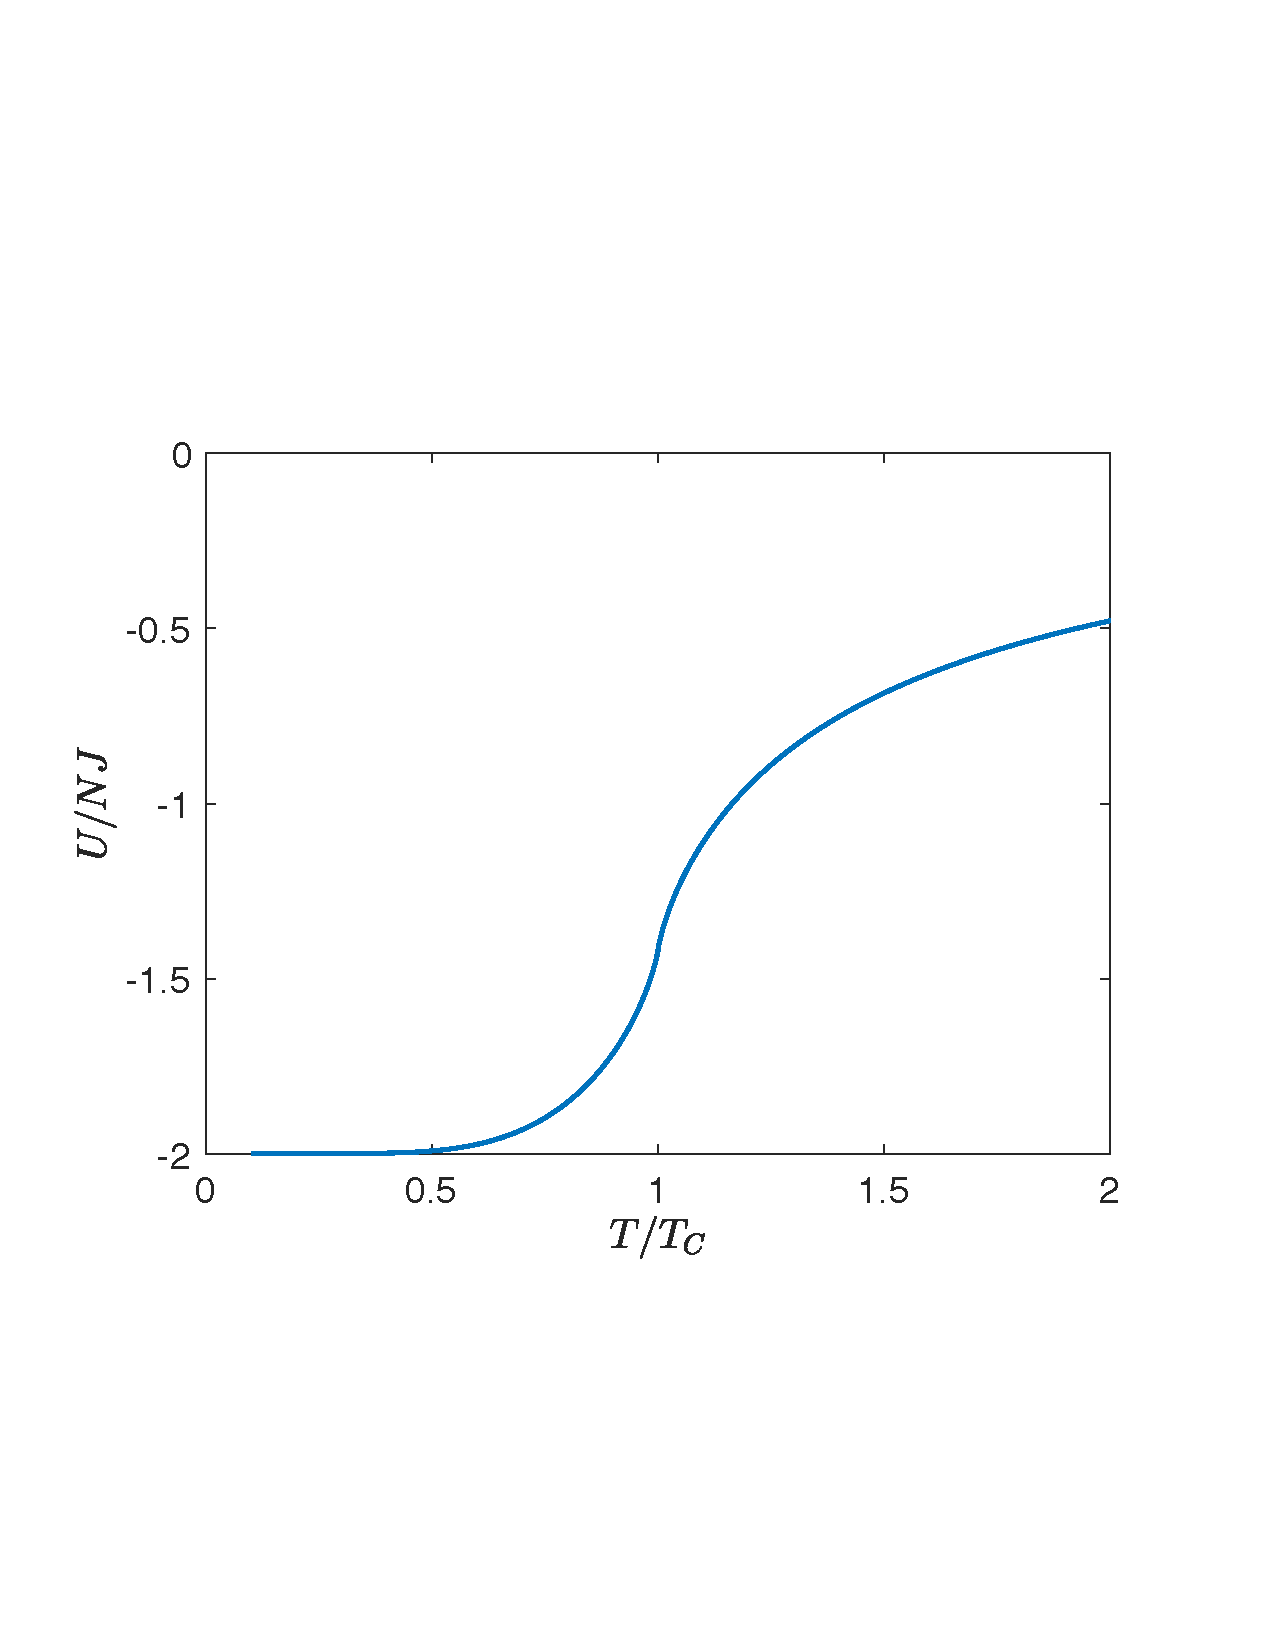
\includegraphics[width=0.53\textwidth]{ising_internal_energy}} 
\subfigure[Entropy.]{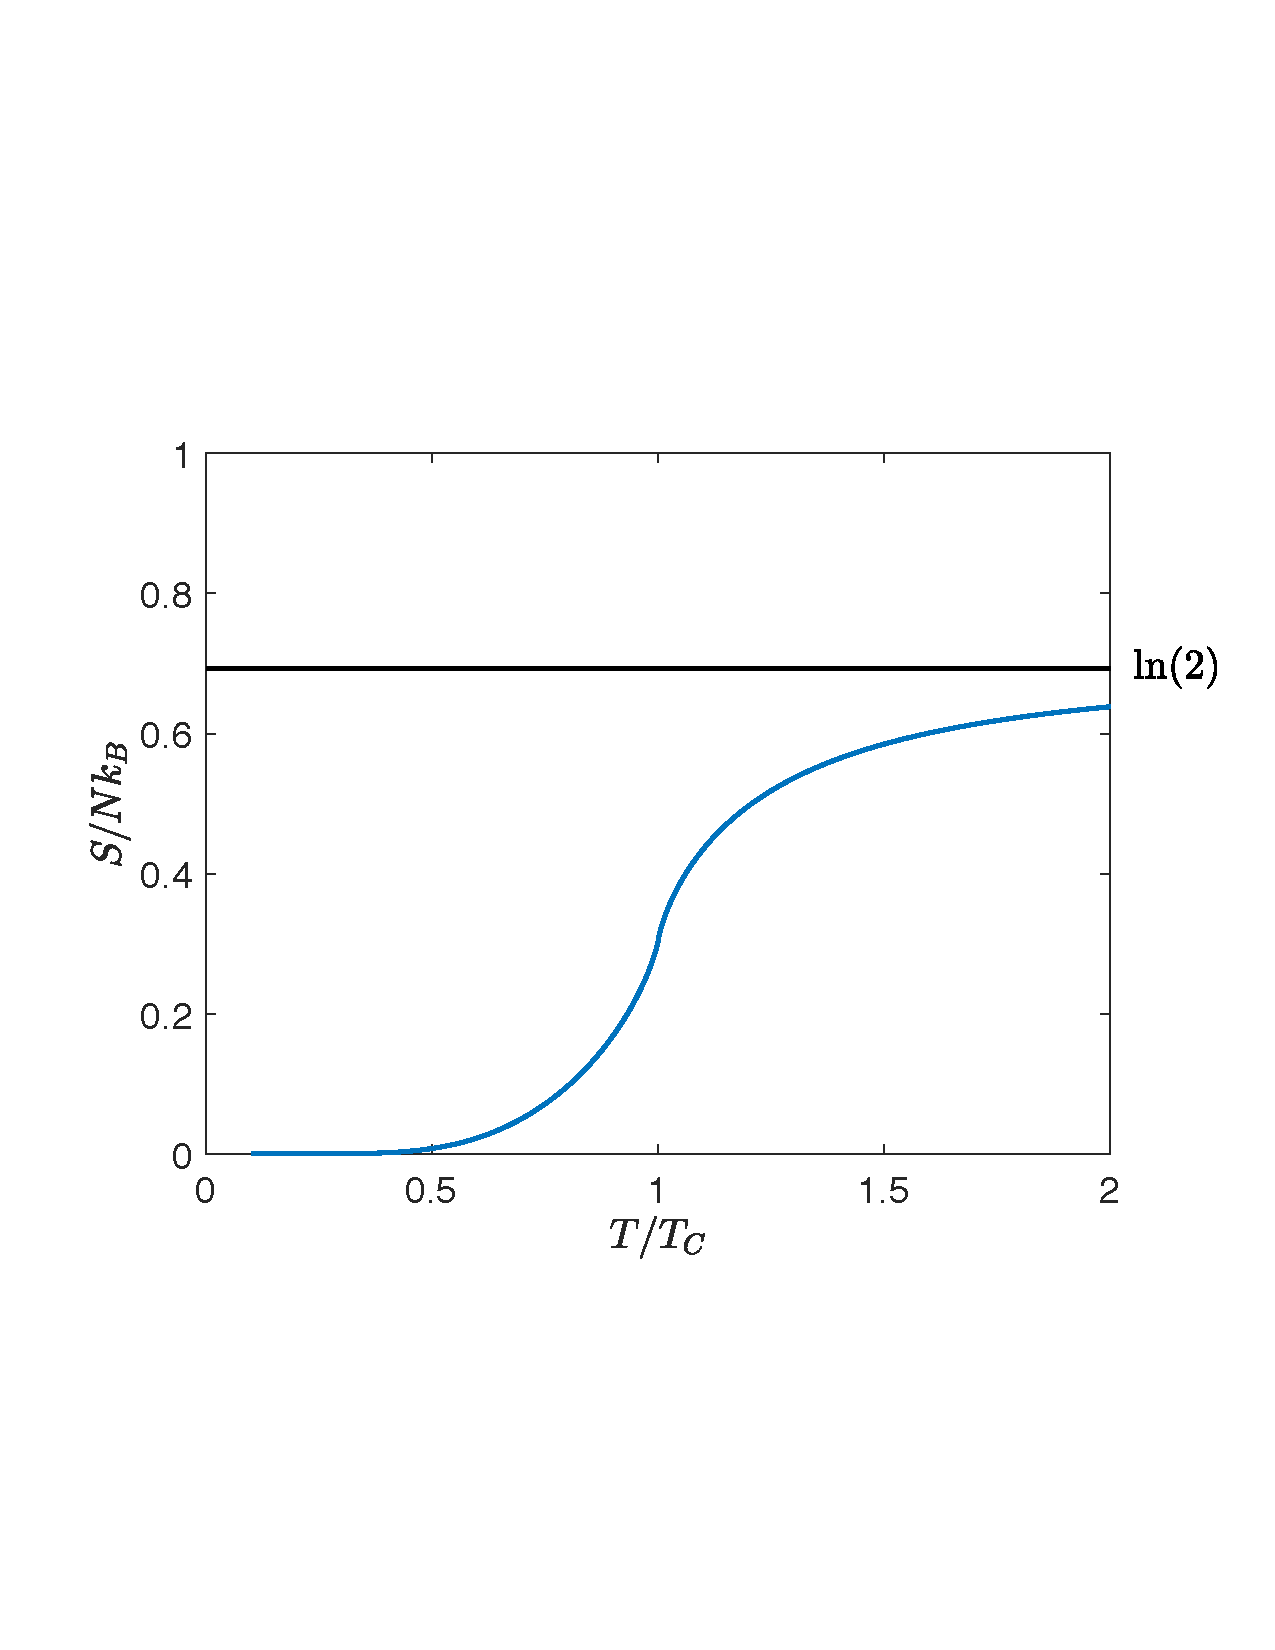
\includegraphics[width=0.55\textwidth]{ising_entropy}} 
\caption{{\it 2d Ising model for $B=0$.}\label{fig:graph:ising:int:energy}}
\end{figure}




\subsection{Entropy}
%
%

%

From $F=U-TS$ we get
\begin{align*}
\frac{S}{N k_{B}} &= j \frac{U}{N J} - \beta \frac{F}{N }
= j \bigg(\frac{U}{N J} \bigg)+\bigg( \frac{\ln(Z)}{N}\bigg)\;.
\end{align*}
%
Hence, we  can express the entropy in terms of \eq{eq:ising:U} and 
\eq{eq:ising:ln:Z}.


We see no critical behaviour in the entropy, which is   the first derivative of the free energy w.r.t. $T$. The latter is continuous at $T_{C}$. According to 
\SEC{sec:ehrenfest:classification} it is therefore not a first order phase transition.

\subsection{Specific heat \label{sec:Ising:2D:spec:heat}}

The order of the phase transition can also be inferred from the specific heat at $B=0$.
%
\begin{align*}
\frac{C}{N} &= \frac{1}{N}\pder{U}{T}{N} 
=\frac{1}{N} \frac{\partial U}{\partial \kappa} 
\underbrace{
\frac{\partial \kappa}{\partial \beta }
}_{\color{blue} =   2J \sqrt{1+\kappa^{2}} }
\underbrace{
\frac{\partial \beta}{\partial T}
}_{\color{blue} = -\frac{1}{k_{B}T^{2}} }\\
&= 
\bigg[\frac{\partial}{\partial \kappa}\bigg(- J g'(\kappa) \sqrt{1+\kappa^{2}} \bigg)\bigg]\;
\bigg(-k_{B}\beta^{2}\big( 2J \sqrt{1+\kappa^{2}} \big)  \bigg)
\end{align*}
%
The final result reads
%

\begin{subequations}\label{eq:spec:heat:2d:ising}
\begin{align}
\frac{C(T)}{N k_{B}}&= 2 j^{2}\;\bigg[\big(1+\kappa^{2} \big)  
 g''(\kappa) + \kappa g'(\kappa) \bigg]\;.
%
\intertext{with}
%
g'(\kappa) &=
\avg{
\frac{2\kappa +\varepsilon}{(1-\kappa)^{2}+\kappa(2+\varepsilon)}
}\\
g''(\kappa) &=
\avg{
\frac{2}{(1-\kappa)^{2}+\kappa(2+\varepsilon)}
}
-
\avg{
\bigg(\frac{2\kappa +\varepsilon}{(1-\kappa)^{2}+\kappa(2+\varepsilon)}\bigg)^{2}
}
\end{align}
\end{subequations}
%
We see in \fig{fig:spec:heat:2d:ising} that the specific heat diverges at $T_{C}$.
In order to unravel the type of divergency we perform a Taylor expansion
in $T$ about $T_{C}$, i.e. $T = T_{C}+\Delta T$. This corresponds to
%
\begin{align*}
j &=j_{C} + \Delta j\\
\kappa &=\sinh(2 J_{C}) + \Delta \kappa = 1  +  \Delta \kappa 
\end{align*}
%
In the last step we have used \eq{eq:jC:2d:ising}.
%
The only divergent behaviour  can come from $g'$ or $g''$.
The other terms can, therefore,  be replaced by $T=T_{C}$. I.e.
\begin{align*}
\frac{C(T_{C}+\Delta T)}{N k_{B}}&= 2 j_{C}^{2}\;
\big[2  g''(\kappa_{c}+\Delta\kappa) + g'(\kappa_{c}+\Delta\kappa) \big]\;.
\end{align*}
%
\begin{figure}[t]
\begin{center}
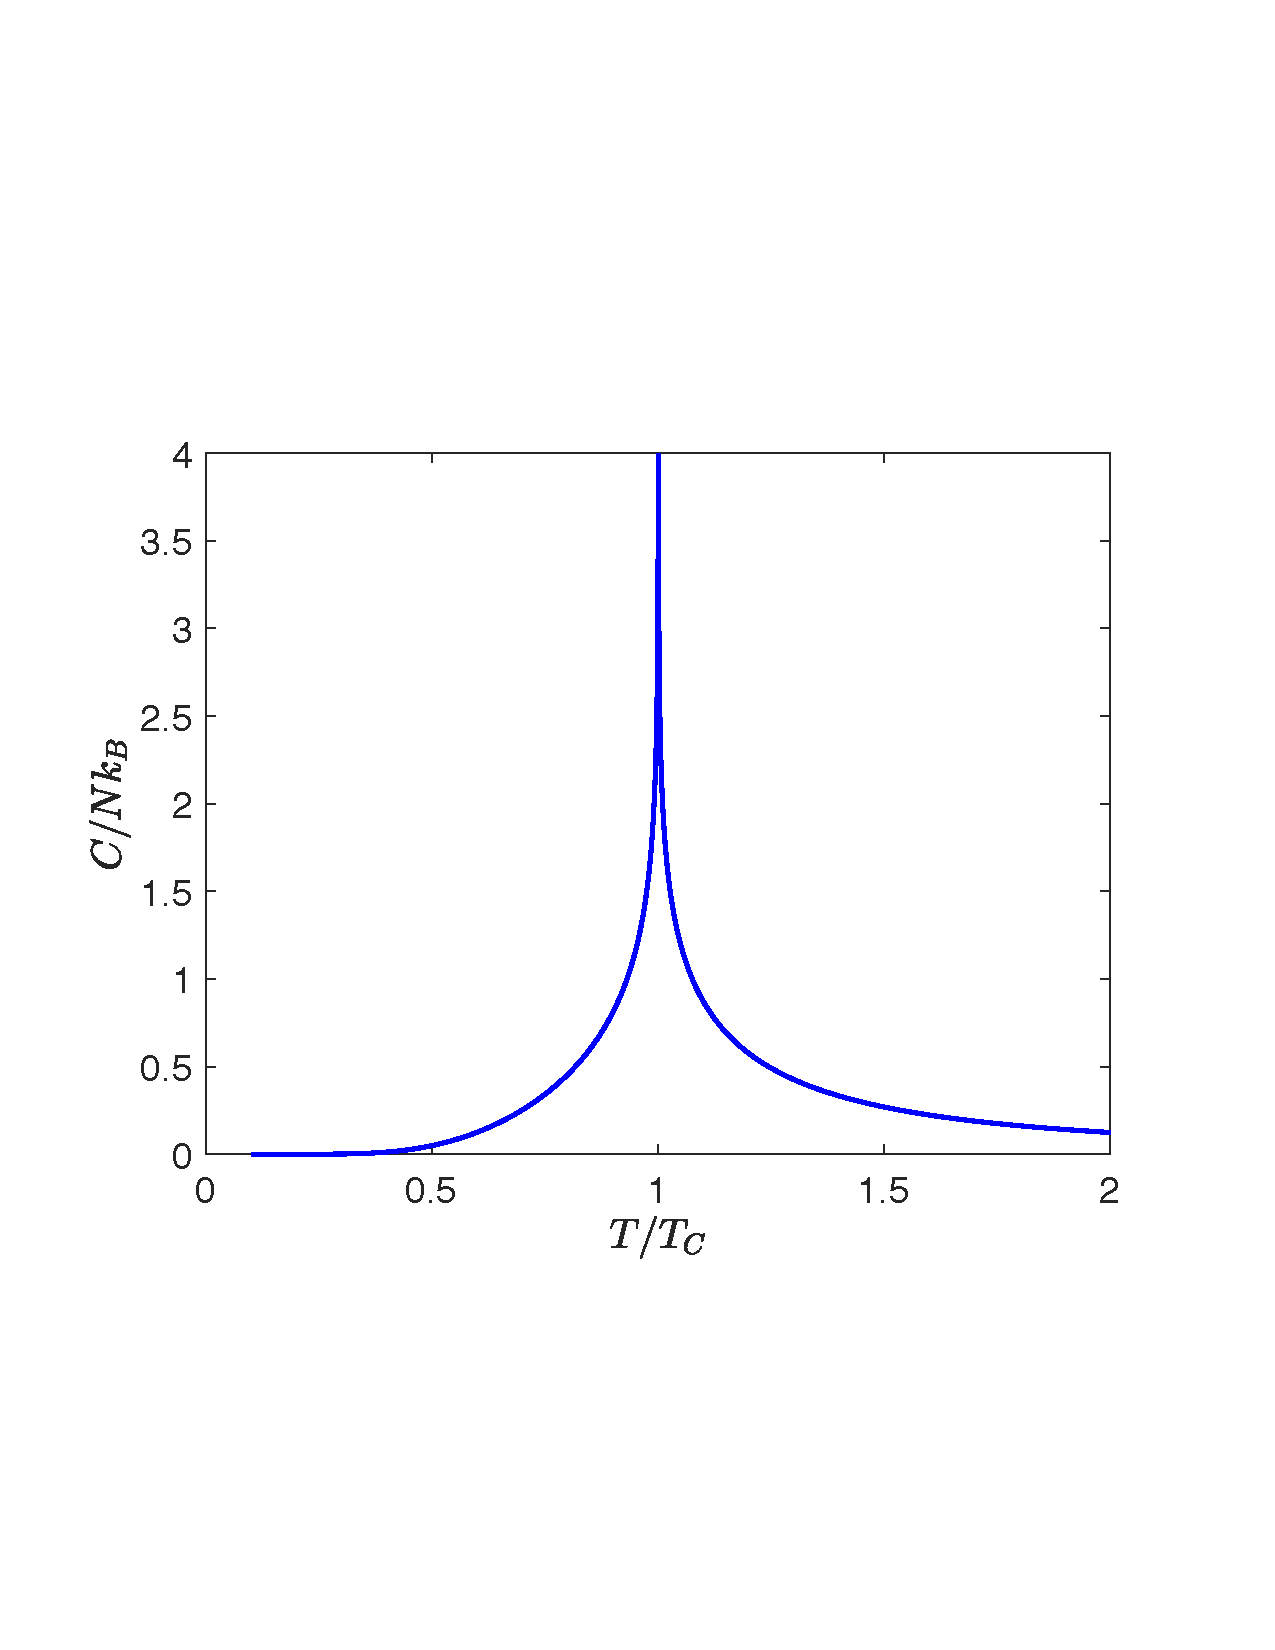
\includegraphics[width=9cm]{ising_spec_heat}
\caption{{\it Specific heat of the 2d Ising model.\label{fig:spec:heat:2d:ising}}}
\end{center}
\end{figure}
There is a critical behaviour in the second derivative of $F$, i.e. the specific heat. Therefore, the Ising model has \blue{a second order phase transition}.
\newpage

\subsubsection{Type of divergency}
The divergency originates from the term $\frac{1}{(1-\kappa)^{2}+\kappa(\varepsilon+2)}$ at the vicinity of  $\varepsilon=-2$.
The dos $\rho(\varepsilon)$ in principle also has a divergency at $\varepsilon=0$ but it is integrable and does not result in a divergence
in the specific heat.
To study the divergency at $\varepsilon=-2$ we split 
%
\begin{align*}
\rho(\varepsilon) &= \underbrace{
\rho(-2)
}_{\color{blue} = \rho_{0}}  + \Delta \rho(\varepsilon)\;.
\end{align*}
%
Then the expectation values become
%
\begin{align*}
\avg{F(\varepsilon)} &= \avg{F(\varepsilon)}_{\rho_{0}} + 
\avg{F(\varepsilon)}_{\Delta\rho}\;.
\end{align*}
%
The second term cause no divergency, hence  we merely need to consider terms of the form
%
\begin{align}\label{eq:}
\avg{F(\varepsilon)}_{\rho_{0}}\;.
\end{align}
%
\emphasize{Proof}{
%
\begin{align*}
&\lim_{\varepsilon\to -2} \frac{\Delta \rho(\varepsilon)(2+\varepsilon +2 \Delta\kappa)}{(\Delta\kappa)^{2} + (1+\Delta\kappa)\big(\varepsilon+2\big)} \\
&=\lim_{\eta\to 0} \frac{\Delta \rho(-2+\eta )(\eta +2 \Delta\kappa)}{(\Delta\kappa)^{2} + (1+\Delta\kappa)\eta} \\
&\overset{\text{L'Hospital}}{=}\lim_{\eta\to 0}  \frac{\Delta \rho'(-2+\eta )(\eta +2 \Delta\kappa) + \Delta\rho(-2+\eta)  }{(\Delta\kappa)^{2} + (1+\Delta\kappa)\eta} \\
&= \lim_{\eta\to 0}  \frac{(2 \Delta\kappa \Delta \rho'(-2+\eta ) + \Delta\rho(-2+\eta)  }{(\Delta\kappa)^{2} } \\
&= \frac{2}{\Delta\kappa}\underbrace{
 \lim_{\eta\to 0} \Delta \rho'(-2+\eta )
}_{\color{blue} = 0} +  \frac{1 }{(\Delta\kappa)^{2} }  \underbrace{
\lim_{\eta\to 0}  \Delta\rho(-2+\eta) 
}_{\color{blue} = 0}\\
&= 0\;.
\end{align*}
% 
or for $g''$ we need
%
\begin{align*}
&\lim_{\varepsilon\to -2} \Delta \rho(\varepsilon) \bigg(\frac{2+\varepsilon+\Delta\kappa}{\big(\Delta \kappa\big)^{2} + (1+\Delta\kappa) \big(\varepsilon+2\big)}\bigg)^{2}\\
&=\lim_{\eta\to 0}  \frac{\Delta \rho(-2+\eta ) \big(\eta+\Delta\kappa\big)^{2}}{\big(\big(\Delta \kappa\big)^{2} + (1+\Delta\kappa) \eta\big)^{2}}\\
&\overset{L'Hospital}{=}\lim_{\eta\to 0}  \frac{\Delta \rho'(-2+\eta ) \big(\eta+\Delta\kappa\big)^{2}+ 2\Delta \rho(-2+\eta ) \big(\eta+\Delta\kappa\big)}
{2 \big(\big(\Delta \kappa\big)^{2} + (1+\Delta\kappa) \eta\big)\big( 1+\Delta\kappa \big)}\\
&\overset{L'Hospital}{=}\lim_{\eta\to 0}  \frac{\Delta \rho'(-2+\eta ) \big(\Delta\kappa\big)^{2}+ 2\Delta \kappa \Delta \rho(-2+\eta ) }
{2 \big(\big(\Delta \kappa\big)^{2} \big)\big( 1+\Delta\kappa \big)}\\
&=
\frac{ \big(\Delta\kappa\big)^{2}}
{2 \big(\big(\Delta \kappa\big)^{2} \big)\big( 1+\Delta\kappa \big)}
\underbrace{
\lim_{\eta\to 0}  \Delta \rho'(-2+\eta ) 
}_{\color{blue} = 0}
+\frac{ 2\Delta \kappa}
{2 \big(\big(\Delta \kappa\big)^{2} \big)\big( 1+\Delta\kappa \big)}\underbrace{
\lim_{\eta\to 0}  \Delta \rho(-2+\eta )
}_{\color{blue} = 0} \\
&=0\;.
\end{align*}}
%
%% end of proof
% 
For the first term in \eq{eq:spec:heat:2d:ising} we need
%
\begin{align*}
g'(1+\Delta\kappa) &= \avg{\frac{\varepsilon+2+\Delta\kappa}{
(2+\varepsilon)( 1+\Delta\kappa ) +(\Delta\kappa)^{2} }}_{\rho_{0}}\;,
\end{align*}
%
for which we find
\begin{align*}
g'(1+\Delta\kappa) 
&=\frac{1}{1+\Delta\kappa} \cdot 
\left\{
4 \rho_{0} + \Delta\kappa  \rho_{0} \ln\big( 4 \big) - 2 \rho_{0} \Delta\kappa \ln\big( \Delta\kappa \big )  + O\big(\Delta\kappa\big)
\right\}\\
&\underset{\Delta\kappa \to 0}     {\longrightarrow} 4\rho_{0} = O(1)\;.
\end{align*}
\emphasize{Proof}{
First we will transform the denominator 
%
\begin{align*}
(2+\varepsilon)( 1+\Delta\kappa ) +(\Delta\kappa)^{2}  &=
( 1+\Delta\kappa )  \bigg(2+\varepsilon+\frac{(\Delta\kappa)^{2}}{1 +\Delta\kappa} \bigg)\\
&= ( 1+\Delta\kappa )  \bigg(2+\varepsilon+ (\Delta\kappa)^{2} + O((\Delta\kappa)^{3})\bigg)\\
\end{align*}
Then
%
\begin{align*}
&\frac{\varepsilon+2+\Delta\kappa}{
(2+\varepsilon)( 1+\Delta\kappa ) +(\Delta\kappa)^{2} } \\
&=\frac{1}{1+\Delta\kappa} \cdot 
\frac{\varepsilon+2+\Delta\kappa}{2+\varepsilon+ (\Delta\kappa)^{2} + O((\Delta\kappa)^{3}}\\
&=\frac{1}{1+\Delta\kappa} \cdot 
\frac{\varepsilon+2+(\Delta\kappa)^{2} + O((\Delta\kappa)^{3}) + \Delta\kappa\big( 1-\Delta\kappa \big)   +O((\Delta\kappa)^{3})  }{2+\varepsilon+ (\Delta\kappa)^{2} + O((\Delta\kappa)^{3})}\;.
\end{align*}
%
I.e.
%
\begin{align}\label{eq:aux:a}
\frac{\varepsilon+2+\Delta\kappa}{
(2+\varepsilon)( 1+\Delta\kappa ) +(\Delta\kappa)^{2} } 
&=\frac{1}{1+\Delta\kappa} \cdot 
\left\{ 1 + \frac{ \Delta\kappa\big( 1-O\big((\Delta\kappa)^{2}\big) \big)   }{2+\varepsilon+ (\Delta\kappa)^{2}\big(1 + O(\Delta\kappa)\big)}\right\}\;.
\end{align}
%
So we have
%
\begin{align*}
&g'(1+\Delta\kappa) = \avg{\frac{\varepsilon+2+\Delta\kappa}{
(2+\varepsilon)( 1+\Delta\kappa ) +(\Delta\kappa)^{2} }}_{\rho_{0}}\\
&=\frac{1}{1+\Delta\kappa} \cdot 
\left\{\avg{1}_{\rho_{0}} + 
\Delta\kappa\big( 1-O\big((\Delta\kappa)^{2}\big) \big) \avg{\frac{1}{2+\varepsilon+ (\Delta\kappa)^{2}\big(1 + O(\Delta\kappa)\big)}}_{\rho_{0}}\right\}\\
\end{align*}
%
The definition of the expectation value is
%
\begin{align*}
\avg{f(\varepsilon)}_{\rho_{0}} &:= \int_{-2}^{2} f(\varepsilon) \rho_{0} d\varepsilon\;
= \rho_{0}\int_{-2}^{2} f(\varepsilon) d\varepsilon\;.
\end{align*}
%
Therefore
%
\begin{align*}
\avg{1}_{\rho_{0}} &= 4 \rho_{0}\;.
\end{align*}
%
%
\begin{align*}
& \avg{\frac{1}{2+\varepsilon+ (\Delta\kappa)^{2}\big(1 + O(\Delta\kappa)\big)}}_{\rho_{0}}\\&=
 \rho_{0}
\int_{-2}^{2}
\frac{1}{2+\varepsilon+ (\Delta\kappa)^{2}\big(1 + O(\Delta\kappa)\big)} d\varepsilon\\
&=\rho_{0} \ln\bigg( 2+2+(\Delta\kappa)^{2}\big(1 + O(\Delta\kappa)\big) \bigg)
-\rho_{0} \ln\bigg( 2-2+(\Delta\kappa)^{2}\big(1 + O(\Delta\kappa)\big) \bigg)\\
&=\rho_{0} \ln\big( 4\big) 
-\rho_{0} \ln\big( \Delta\kappa)^{2}\big)  + O\big(\Delta\kappa\big)
\end{align*}
%
In total we have
%
\begin{align*}
&g'(1+\Delta\kappa) = \avg{\frac{\varepsilon+2+\Delta\kappa}{
(2+\varepsilon)( 1+\Delta\kappa ) +(\Delta\kappa)^{2} }}_{\rho_{0}}\\
&=\frac{1}{1+\Delta\kappa} \cdot 
\left\{
4 \rho_{0} + \Delta\kappa  \rho_{0} \ln\big( 4 \big) - 2 \rho_{0} \Delta\kappa \ln\big( \Delta\kappa \big )  + O\big(\Delta\kappa\big)
\right\}\\
&\underset{\Delta\kappa \to 0}     {\longrightarrow} 0\;.
\end{align*}
}
%
% end oif proof

Similarly, for the second term of $g''$ we  find with \eq{eq:aux:a}
%
\begin{align*}
&\avg{
\bigg(\frac{2\kappa +\varepsilon}{(1-\kappa)^{2}+\kappa(2+\varepsilon)}\bigg)^{2}
}_{\rho_{0}}\\
 &= \bigg(\frac{1}{1+\Delta\kappa} \bigg)^{2}\cdot 
\avg{\bigg(1 + \frac{ \Delta\kappa\big( 1-O\big((\Delta\kappa)^{2}\big) \big)   }{2+\varepsilon+ (\Delta\kappa)^{2}\big(1 + O(\Delta\kappa)\big)}\bigg)^{2}}_{\rho_{0}}\\
&= O(1) + O(\Delta\kappa \ln(\Delta\kappa)) + O\big(\big(\Delta\kappa\big)^{2}\big)\int_{-2}^{2} \frac{1}{2+\varepsilon+\big(\Delta\kappa  \big)^{2}}d\varepsilon\\
&= O(1) + O(\Delta\kappa \ln(\Delta\kappa)) + O\big(\big(\Delta\kappa\big)^{2}\big)
\bigg( O(1) + O\big( \frac{1}{(\Delta\kappa)^{2}} \big) \bigg)\\
&=  O(\Delta\kappa \ln(\Delta\kappa))+O(1) + O(\big( (\Delta\kappa)^{2} \big)
\end{align*}
%
Again no divergency.
The only divergent term stems from the first part of $g''$, which yields
%
\begin{align*}
&\avg{\frac{2}{(\Delta\kappa)^{2}+(1+\Delta\kappa)(2+\varepsilon)}}_{\rho_{0}} 
=
\int_{-2}^{2} \frac{\rho_{0} }{(\Delta\kappa)^{2}+(1+\Delta\kappa)(2+\varepsilon)} d\varepsilon\\
&= \rho_{0} \ln\big[ (\Delta\kappa)^{2}+(1+\Delta\kappa)(2+2) \big]
-
\rho_{0} \ln\big[ (\Delta\kappa)^{2}+(1+\Delta\kappa)(2-2) \big]\\
&= \rho_{0} \ln\big[ 4 + O\big(\Delta\kappa\big) \big]
-
2 \rho_{0} \;\ln(\abs{\Delta\kappa});\\
&=O(1)  - 2 \;\ln(\abs{\Delta\kappa});
\end{align*}
%
The specific heat obviously has a logarithmic divergency, which corresponds
to the critical exponent
%
\begin{align}
\alpha &=\alpha' = 0\;.
\end{align}
%
For the definition of the critical exponents see \SEC{sec:critical:exponents}.

%
\subsection{Spontaneous magnetization}
So far it has not been possible to find the exact solution of the 2d Ising model in an external magnetic
field. This is only doable for infinitesimal $B$ values, which is enough to determine the spontaneous 
magnetization. It amounts to computing the spin-spin correlation $\langle S_{i} S_{j}\rangle$ and use
%
\begin{align*}
\lim_{l\to\infty} \langle S_{i}  S_{i+l}\rangle \longrightarrow \bigg(  \langle S_{i} \rangle\bigg)^{2}
= \bigg(\frac{M}{N }\bigg)^{2}\;.
\end{align*}
%
The graphical solution amounts to count all graphs as before but with the peculiarity that 
the vertices $i$ and $j$ have an odd order.
The result reads
\tboxit{Spontaneous Magnetization of the 2d Ising Model}{
%
\begin{align}\label{eq:}
\frac{M}{N}&=
\begin{cases}
	\big( 1-\sinh^{-4}(2 j) \big)^{1/8}&\text{for } T\le T_{C}\\
	0&\text{otherwise}
\end{cases}
\end{align}
%
}
The order parameter, the magnetization, is continuous, which corroborates 
the statement, that it is a second order phase transition.
%
\begin{figure}[t]
\begin{center}
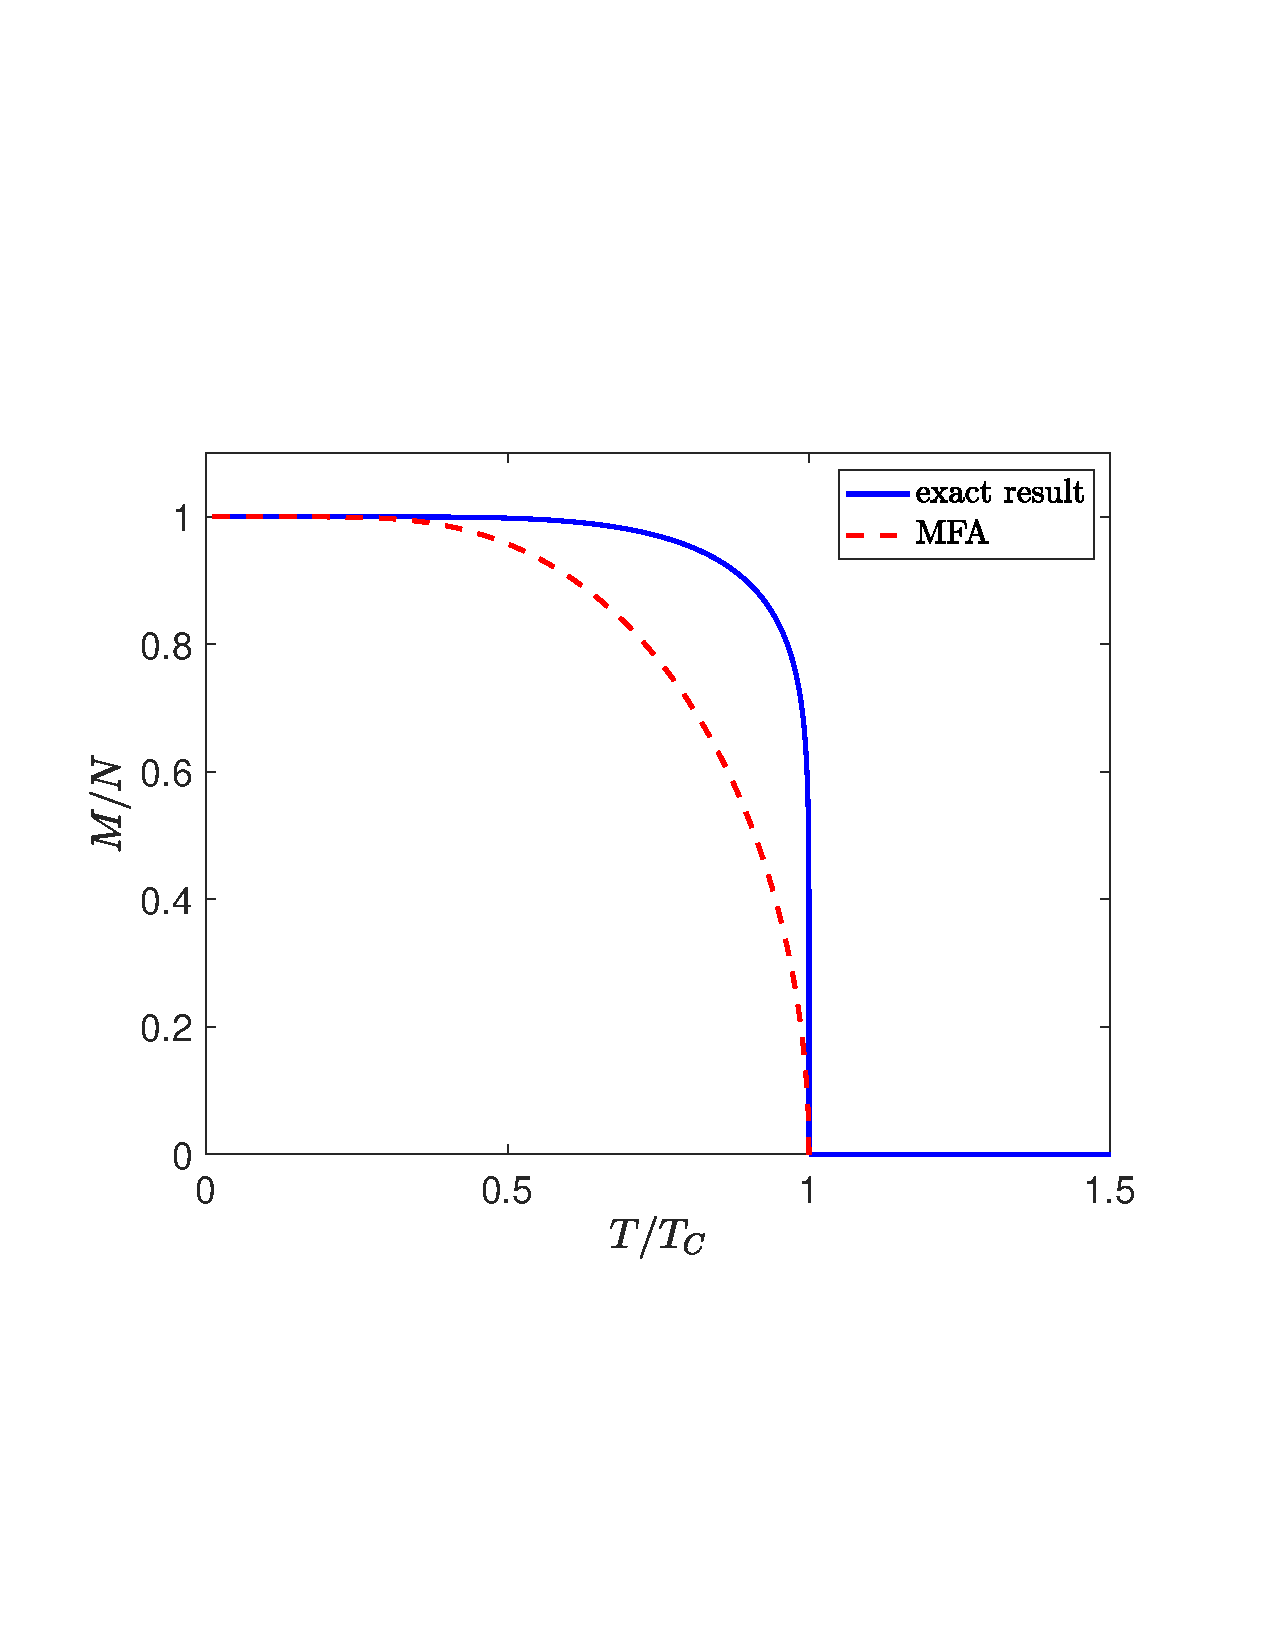
\includegraphics[width=9cm]{ising_magnetization}
\caption{{\it Spontaneous magnetization of Ising spins.}}
\end{center}
\end{figure}
%

%
\subsection{Proof}

We seek the number of paths from the center $\vv x=0$ to site $\vv x$, where the Manhattan distance is 
$n$. We consider only cases with $n>1$, actually we are interested in $n-1$ to $\infty$. 
We are interested in the weighted sum over all paths from the center to site $\vv x$. Schematically this can be written as
%
\begin{align*}
Z_{0 \vv x} &= \sum_{m=n}^{\infty}  W^{(m)}_{0,\vv x}\;,
\end{align*}
%
where $W^{(m)}_{0,\vv x}$ stands for the contributions that contain $m$ steps. We will again use the previous matrix $M^{(m)}$. Here, however, we are not counting loops and therefore the weights are not entirely correct
and it is not yet clear what we have to do with the directions of the last step, which points from the final point $\vv x$ to an arbitrary direction. It is, therefore, useful, to split off the last step. Then it seem reasonable to 
start with the form
%
\begin{align*}
W^{(m)}_{0,\vv x} &= \sum_{\vv d_{0}} \sum_{\vv x',\vv d'}  \bigg(M^{(m-1})\bigg)_{(\vv 0,\vv d_{0}),(\vv x',\vv d')}  \big(M^{(1)}\big)_{(\vv x',\vv d'),(\vv x,\vv d'')}
\end{align*}
%
There is one constraint:
%
\begin{align*}
\vv x'  &= \vv x - \vv d'\;.
\end{align*}
%
The last term adds a factor $th(j)$ plus a phase, that depends on the yet undefined $\vv d''$.
The phase-factors are only correct in closed loops to add up to the sign, representing crossings.
Therefore, we will add graph elements to from a closed loop, such that no additional crossings occur.
There are 16 possibilities depending on $\vv d$ and $\\vv d'$
%
%\begin{table}[]
%\begin{tabular}{llllll}
% 1)&  $\vv d = \$  & i.e. a loop is closed  &$\Rightarrow$ &   $f= Straight$  \\
% 2)&  $\vv d'= -\vv d = \vv e \alpha$  & i.e. a loop is closed  &$\Rightarrow$ &   $f= 2 left$  \\
%  3)&  $\vv d'= -\vv d = -\vv e \alpha$  & i.e. a loop is closed  &$\Rightarrow$ &   $f= 2 right$  \\
%   4)&  $\vv d'= -\vv d = \vv e x$  & i.e. a loop is closed  &$\Rightarrow$ &   $f= LL$  \\
% &  &  &  &  \\
% &  &  &  & 
%\end{tabular}
%\end{table}
%
%
%
%kerze


\subsection{Critical exponent \label{sec:Ising:2D:beta}}
For  $T\searrow T_{C}$ we have
%
\begin{align*}
\frac{M}{N} &= \bigg( 1 - \big[\sinh\big( 2 j_{C} + 2J\Delta \beta  \big)\big]^{-4} \bigg)^{\frac{1}{8}}\\
&= \bigg( 1 - \underbrace{
\big[\sinh\big( 2 j_{C}\big)
}_{\color{blue} \overset{(\ref{eq:jC:2d:ising})}{=} 1} + \cosh\big(2j_{C}  \big) J\Delta \beta\big]^{-4} \bigg)^{\frac{1}{8}}\;.
\end{align*}
%
In addition, we have 
%
\begin{align*}
\cosh\big( 2 j_{C} \big) &= \sqrt{1+\sinh^{2}(2 j_{C})} = \sqrt{2}\;.
\end{align*}
%
Hence
%
\begin{align*}
\frac{M}{N} &=\bigg( 1 - \big[ 1 + \sqrt{2} J \Delta\beta \big]^{-4} \bigg)^{\frac{1}{8}}\\
&=\bigg( 1 - 1 +4\sqrt{2}  J \Delta\beta  \bigg)^{\frac{1}{8}}\\
&=\bigg(4\sqrt{2}  J \Delta\beta  \bigg)^{\frac{1}{8}}\\
&=\propto  \big(\frac{1}{T}-\frac{1}{T_{C}}\big)   ^{\frac{1}{8}}\\
&\propto \varepsilon^{\frac{1}{8}}
\end{align*}
%


	

%\chapter{Ising a la Samuel}
\section{Grassmann variables}


\newcommand{\mode}{flavor }
\newcommand{\modes}{flavors }
\newcommand{\hdag}[1]{h^{x}_{#1}}
\newcommand{\vdag}[1]{v^{x}_{#1}}
\newcommand{\hnag}[1]{h^{o}_{#1}}
\newcommand{\vnag}[1]{v^{o}_{#1}}
\newcommand{\Hdag}[1]{H^{x}_{#1}}
\newcommand{\Vdag}[1]{V^{x}_{#1}}
\newcommand{\Hnag}[1]{H^{o}_{#1}}
\newcommand{\Vnag}[1]{V^{o}_{#1}}

\newcommand{\cP}{{\cal P}}
\newcommand{\sign}[1]{\text{sgn}\left\{#1\right\}}



%\newcommand{\hdag}[1]{h^{\dagger}_{#1}}
%\newcommand{\vdag}[1]{v^{\dagger}_{#1}}
%\newcommand{\hnag}[1]{h^{\phantom{\dagger}}_{#1}}
%\newcommand{\vnag}[1]{v^{\phantom{\dagger}}_{#1}}

\renewcommand{\xx}[1]{\boldsymbol  x_{#1}}
\newcommand{\ex}{\boldsymbol  e_{x}}
\newcommand{\ey}{\boldsymbol  e_{y}}

\newcommand{\Dep}{{\cal D}_{\eta \psi}}
\newcommand{\Dept}{\tilde {\cal D}_{\eta \psi}}
\newcommand{\Depx}{{\cal D}_{\eta \psi}^{\canceledk{I},\canceledk{J}}}
\newcommand{\Deta}{{\cal D}_{\eta}}
\newcommand{\Detax}{{\cal D}_{\eta}^{\canceledk{I}}}
\newcommand{\Detat}{\tilde {\cal D}_{\eta}}
\newcommand{\Dxi}{{\cal D}_{\xi}}

\newcommand{\Int}{\int\ldots\int}
\newcommand{\Disingi}{{\cal D}_{hv}}
\newcommand{\Pf}[1]{\text{Pf}\left(#1\right)}
\newcommand{\Det}[1]{\text{det}\left(#1\right)}

\newcommand{\set}[2]{\left\{#1_{1},#1_{2},\ldots,#1_{#2}\right\}}
\newcommand{\pairset}[3]{\left\{(#1_{1},#2_{1}),(#1_{2},#2_{2})\ldots,(#1_{#3},#2_{#3})\right\}}

\newcommand{\Set}[2]{\left\{#1_{l}\right\}_{l=1:#2}}
\newcommand{\Pairset}[3]{\left\{(#1_{l},#2_{l})\right\}_{l=1:#3}}



\newcommand{\compset}[3]{#1_{1} #2 #1_{2} #2 \ldots #2 #1_{#3}}

\newcommand{\setprod}[4]{#1_{#2_{1}#3_{1}}\;#1_{#2_{2}#3_{2}}\;\ldots\;  #1_{#2_{#4}#3_{#4}}}
\newcommand{\Setprod}[4]{\prod_{l=1}^{#4}\;#1_{#2_{l}#3_{l}}}


To allow for all elements for admissible graphs we introduce per site 4 
Grassmann variables, two for each direction
$\hdag{i},\hnag{i},\vdag{i},\vnag{i}$, where the first two are for the horizontal direction
and the second two for vertical direction. These are 4 independent variables. Let $\eta $ stand for one of theses variables, then they fulfill
%
\begin{align*}
\int d \eta  &= 0\; \\
\int d \eta  \eta &= 1\\
\eta^{2} &= 0
\end{align*}
%
%
We introduced the trace ($\text{tr}$), which means
%
\begin{subequations}\label{eq:Disingi}
\begin{align}
\tr {f(\{\hdag{i},\hnag{i},\vdag{i},\vnag{i}\})} &= \Int \Disingi\;f(\{\hdag{i},\hnag{i},\vdag{i},\vnag{i}\})\\
\Disingi &= \prod_{i}   d\hdag{i} d \hnag{i}, d\vdag{i},d \vnag{i}
\end{align}
\end{subequations}
%
In particular for a single pair of GV at one site we have
%
\begin{align}
\int\int d \hdag{i} d \hnag{i}  \hnag{i} \hdag{i} &=
\underbrace{
\int d \hdag{i} \hdag{i}
}_{\color{blue} = 1} \underbrace{
\int d \hnag{i}  \hnag{i} 
}_{\color{blue} = 1} = 1\;,
\end{align}
%
but
%
\begin{align}
\int\int d \hdag{i} d \hnag{i}   \hdag{i} \hnag{i}&= -
\underbrace{
\int d \hdag{i} \hdag{i}
}_{\color{blue} = 1} \underbrace{
\int d \hnag{i}  \hnag{i} 
}_{\color{blue} = 1} = -1\;.
\end{align}
%
Obviously, at each site all four GVs have to be present, otherwise the trace over all GVs vanishes.
\clearpage 
We introduce the following graphical meaning for the GV
\begin{figure}[h]
\begin{center}
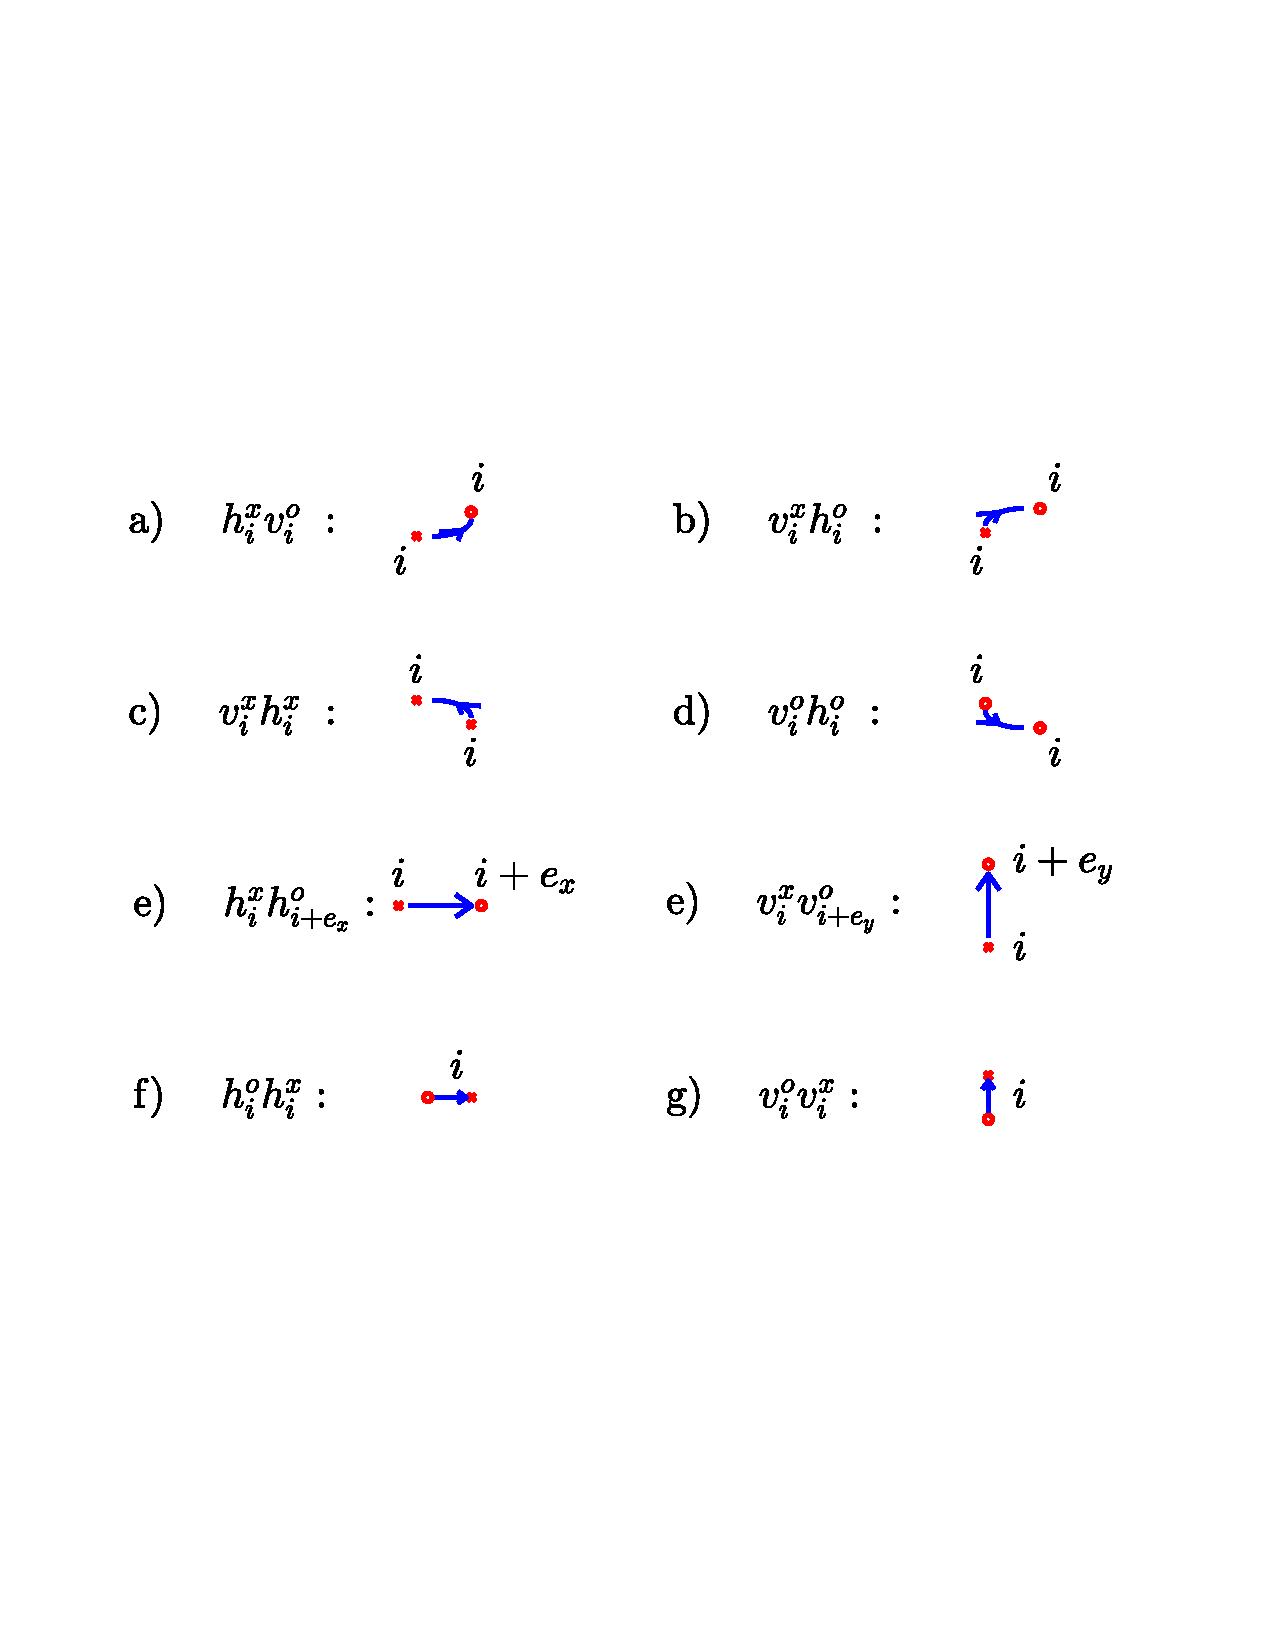
\includegraphics[width=10cm]{GV_pairs}
\caption{{\it The 6 GV-pairs that form the graph elements.}\label{fig:GV_pairs}}
\end{center}
\end{figure}
%

Then we introduce an  action with theses elements
%

\begin{subequations}\label{eq:}
\begin{align}
A &= A_\text{bonds}  + A_\text{corners}  + A_\text{monomers}\\
A_\text{bonds} &= t \sum_{i} \bigg( \hdag{\xx{i}} \hnag{\xx{i}+\ex }
+ \vdag{\xx{i}} \vnag{\xx{i}+\ey}\bigg)\\
A_\text{corners} &=  -\sum_{i} \bigg(\hdag{\xx{i}} \vnag{\xx{i}}+\vdag{\xx{i}} \hnag{\xx{i}}
+\vdag{\xx{i}} \hdag{\xx{i}} 
+\vnag{\xx{i}} \hnag{\xx{i}} 
\bigg)\\
A_\text{monomers} &=  -\sum_{i} \big(\hnag{\xx{i}}\hdag{\xx{i}}
+\vnag{\xx{i}} \vdag{\xx{i}}\big) \\
A&=\sum_{i=1}^{N}  \sum_{\nu=1}^{n_{i}} P_{i}^{(\nu)}
\end{align}
\end{subequations}
%
These elements are depicted in figure \ref{fig:GV_pairs}.
The reason for the minus signs will be clarified later on.
We can then define a kind of partition function
%
\begin{align*}
Z &= \text{tr} e^{A}\;.
\end{align*}
%
We will show in the sequel that 
%
\begin{align*}
\sum_{G} t^{N_{e}(G)} &= (-1)^{N} Z\;.
\end{align*}
%
Since we have a quadratic action in the GVs, we can compute the partition function analytically.
Due to the Grassmannian properties, the pair-variables fullfill $P^{2}=0$.
When expanding $e^{A}$ we, therefore, obtain
%
%
\begin{align*}
e^{A} &= \prod_{i=1}^{N}  \prod_{\nu=1}^{n_{i}} \big(1 + P_{i}^{(\nu)}\big)\;.
\end{align*}
%
Each GV-pair is of the form
%
\begin{align*}
\eta_{i_{1}}^{\alpha_{1}}\eta_{i_{2}}^{\alpha_{2}}\;,
\end{align*}
%
where the lower index stand for the site  and
the upper (type-)index combines the direction $\{h,v\}$ and the \mode $\{x,o\}$.
So we can suitably combine the the GV-pairs $P_{i}^{(\nu)} $. In doing so, we 
have to keep in mind that  each variable for site $i$, i.e.   
$\{\hdag{\xx{i}},\hnag{\xx{i}},\vdag{\xx{i}},\vnag{\xx{i}} \}$ has to occur once and  only once. 



The graphical elements, required to form admitted graphs, are depicted in 
figure \ref{fig:combinations}.
%
\begin{figure}[h]
\begin{center}
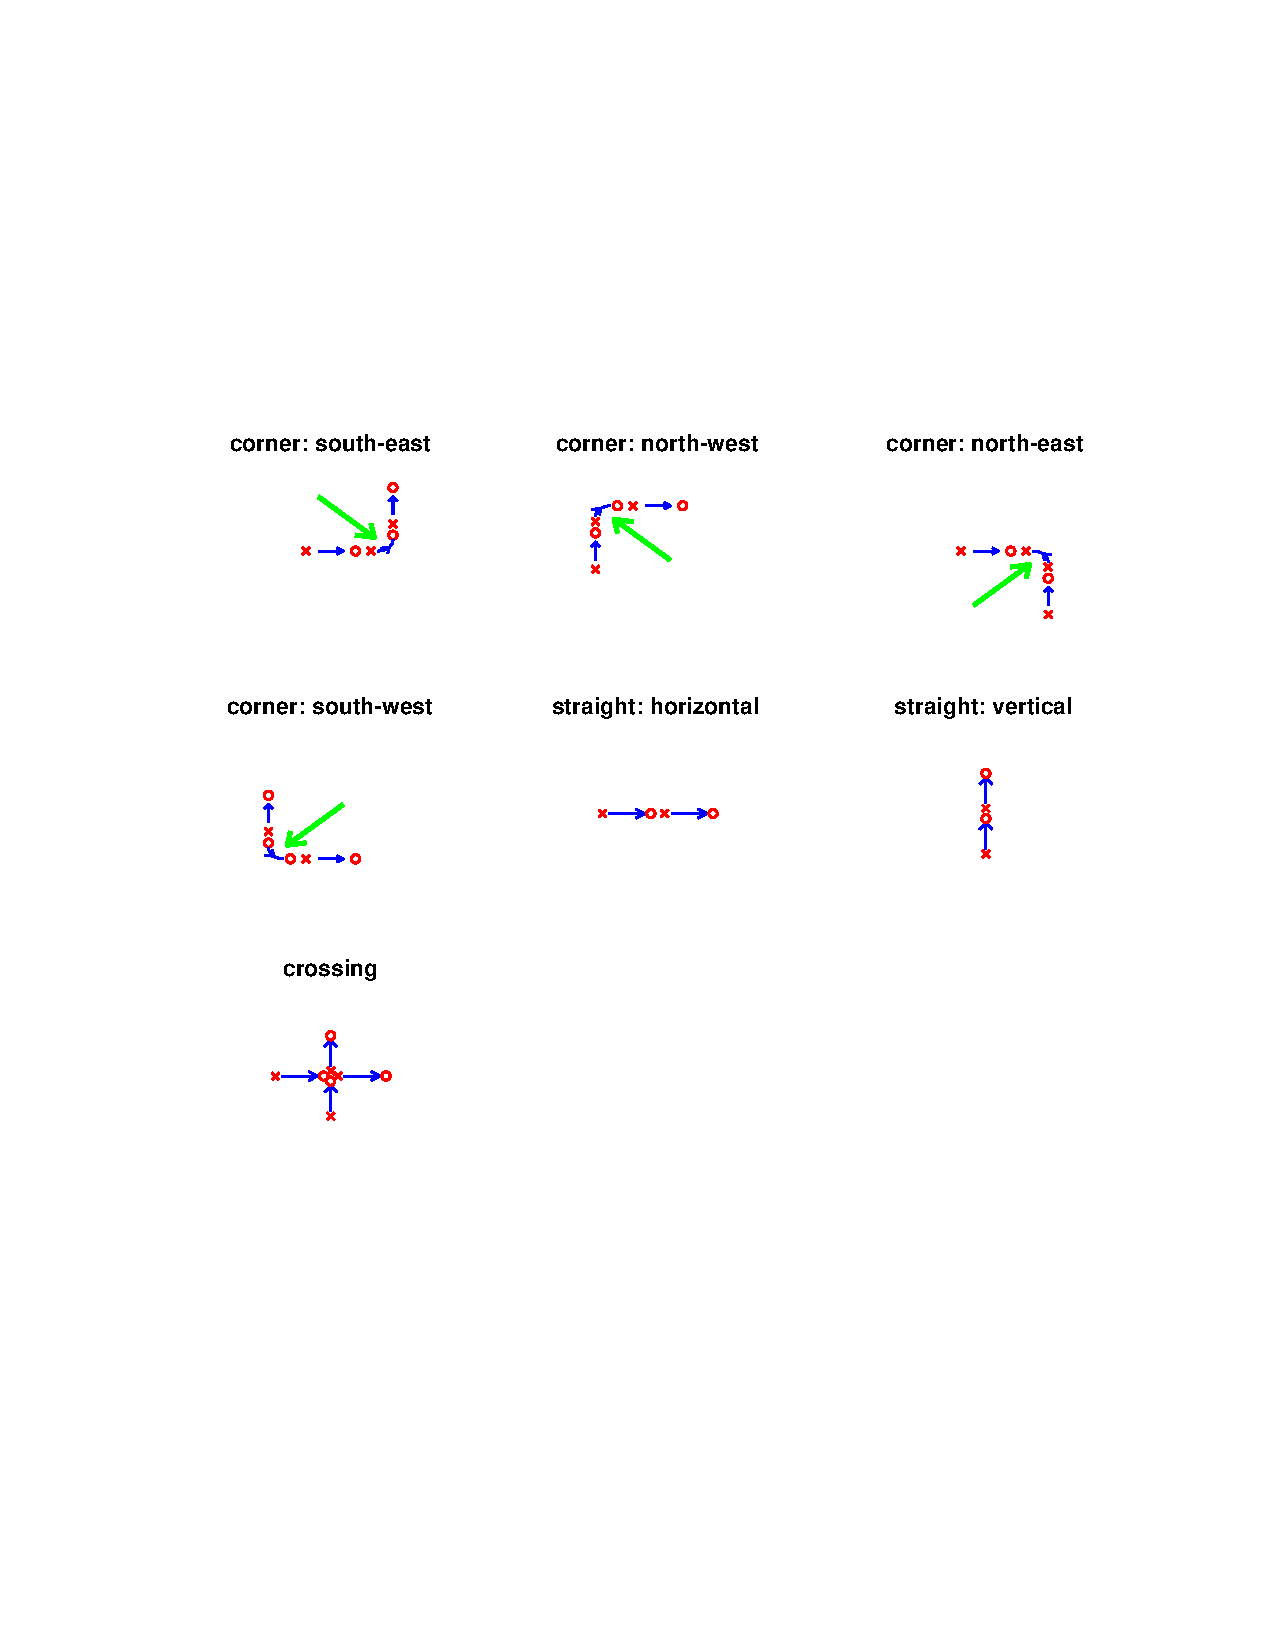
\includegraphics[width=12cm]{path_elements}
\caption{{\it All possible combinations of GV-pairs at one site. Monomers that form empty sites are omitted, as well as monomers, that are needed to complete the straight lines. The elements in these subfigures are the building blocks needed   to form all possible graphs.}\label{fig:combinations}}
\end{center}
\end{figure}
%
These elements are all that is required to form all admitted graphs; and due to the 
Grassmannian properties each graph is generated exactly once. Hence, we have essentially
%
\begin{align*}
\text{tr}\bigg\{ e^{A} \bigg\} &= \sum_{G} \text{sign}(G) t^{N_{e}(G)}\;.
\end{align*}
%
The  factors $t$ are correctly included since each bond is associated with a factor $t$.
We still need to make sure that each admitted graph has the correct sign.
In addition, to the sites that have lines attached to them,
we also need to ensure that empty site are included correctly, i.e. they should only multiply
a factor 1 to each graph.

\subsection{Monomers}
 
The monomers add missing variables, either for empty sites, or those not used  for building the graphs. 

Empty sites can be formed by a monomer pair for the horizontal and one for the vertical
direction, i.e.
%
\begin{align*}
\hnag{\xx{i}} \hdag{\xx{i}}\vnag{\xx{i}}\vdag{\xx{i}}
\end{align*}
%
and the trace gives 
%
\begin{align*}
\underbrace{
\iint d \hdag{\xx{i}} d \hnag{\xx{i}}\hnag{\xx{i}} \hdag{\xx{i}}
}_{\color{blue} = 1}
\cdot\underbrace{
\iint d \vdag{\xx{i}} d \vnag{\xx{i}} \vnag{\xx{i}}\vdag{\xx{i}} 
}_{\color{blue} = 1}&= 1\;.
\end{align*}
%
Also if we include the minus sign in the action, the contribution is $+1$, as the we have $(-1)^{2}$.
Since all GVs at site $i$ are involved, no other GV-pair can occur at site $i$, if there are already the two monomer pairs. 
Alternatively, the product of the GVs of corner a) and b) or  the GVs of corner c) and d)   provide all GVs for site i as well. That yields
%
\begin{align*}
a) \cdot   b) &= \hdag{\xx{i}}\vnag{\xx{i}} \vdag{\xx{i}} \hnag{\xx{i}} =- \hdag{\xx{i}} \hnag{\xx{i}}  \vdag{\xx{i}}\vnag{\xx{i}} 
\end{align*}
%
and the integral gives $-1$. or
\begin{align*}
c) \cdot  d) &=\vdag{\xx{i}}  \hdag{\xx{i}}\vnag{\xx{i}}  \hnag{\xx{i}} =- \hdag{\xx{i}} \hnag{\xx{i}}  \vdag{\xx{i}}\vnag{\xx{i}} \;,
\end{align*}
which also gives $-1$ after the integral.
These 3 terms have to be added, as they all yield an empty site. \blue{So the total weight of an empty site is $-1$}


\begin{figure}[h]
\begin{center}
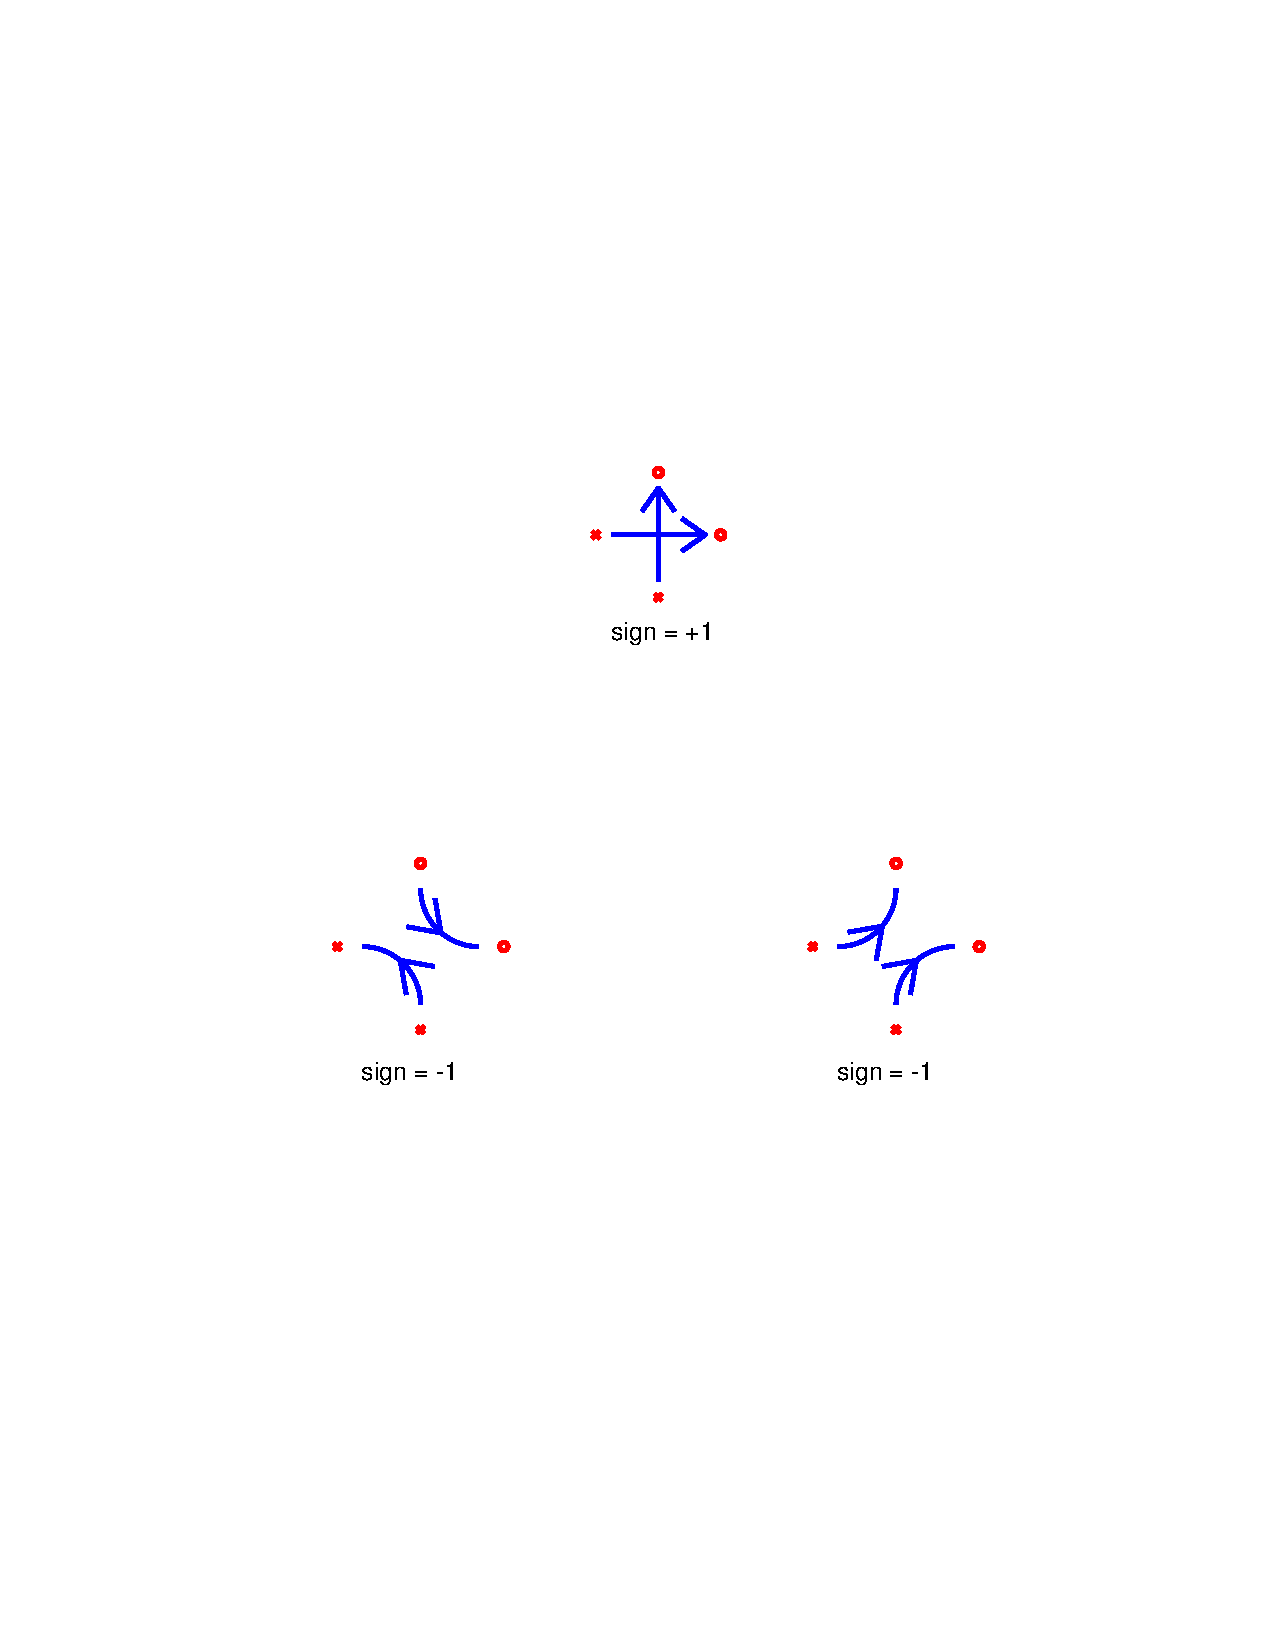
\includegraphics[width=7.5cm]{monomers}
\caption{\it There are three possible combinations of GV-pairs that represent empty sites.
The weights add up to $-1$.\label{fig:empty_sites}}
\end{center}
\end{figure}
%


Next we consider the contribution of a closed loop. It is produced by a suitable product
of GV-pairs 
%
\begin{align*}
\prod_{n=1}^{L}  P_{n}
%\eta_{i^{n}_{1}}^{\sigma^{n}_{1},\alpha^{n}_{1}}\eta_{i^{n}_{2}}^{\sigma^{n}_{2},\alpha^{n}_{2}}\;.
\end{align*}
%
each consisting of two GVs with a site and a type index.

We pick out one  of the bond pairs. It has site indices 
$i_{1}, i_{2}$ and type indices $\alpha_{1},\alpha_{2}$. Then from the remaining set of 
GV-pairs we take the one that contains  in one of its two GVs the site index $i_{2}$ and 
the complement of $\alpha_{2}$, i.e. $\overline \alpha_{2}$. By the complement we mean the opposite \mode value but the same directional value, i.e.
$(h x)\leftrightarrow (h o)$ and $(v x)\leftrightarrow (v o)$. The other variable shall have
site index $i_{3}$ and type index $\alpha_{3}$. 
If the first operator in the second GV-pair is the one that matches the second variable of the first pair, then we have a factor +1 otherwise a factor -1. 

When we use the graphical representation of the GV-pairs, the first is an arrow with an $x$
at its beginning and an $o$ at its end. Now we attache the graphical element of the second GV-pair. The arrow already indicates whether or not the variables are in the required order.
I.e. If we move opposite the arrow direction we get a minus sign. In addition, if the contracted
pair of variables $\eta_{i_{2}}^{\alpha_{2}}$ and $\eta_{i_{2}}^{\overline \alpha_{2}}$
have the \modes $ox$ that the trace gives +1 otherwise for $xo$ we obtain $-1$.
Next, we seek again the pair that now contains site
$i_{3}$ and type $\overline \alpha_{3}$.
Again we obtain a factor -1 if we move opposite the arrow direction and another -1 if the \mode-sequence is $xo$.
Now we move on like this. 
At the last step there is a final dangling (not contracted) variable with site index that has to be equal to $i_{1}$ and a type index equal to $\overline \alpha_{1}$. Otherwise,
the trace   over these the GV-pairs vanishes and they do not form an admitted graph.
By now we have reordered  the blocks of GV pairs (which causes no sign).
Again we obtain the two possible signs. Finally, we move the dangling variable to the front
of the GV-pair product, which gives an additional minus sign. Finally, we analyze the sign of the so-produce \mode sequence at the first variable pair.
%
The procedure is represented in figure \ref{fig:example}.
\begin{figure}[h]
\begin{center}
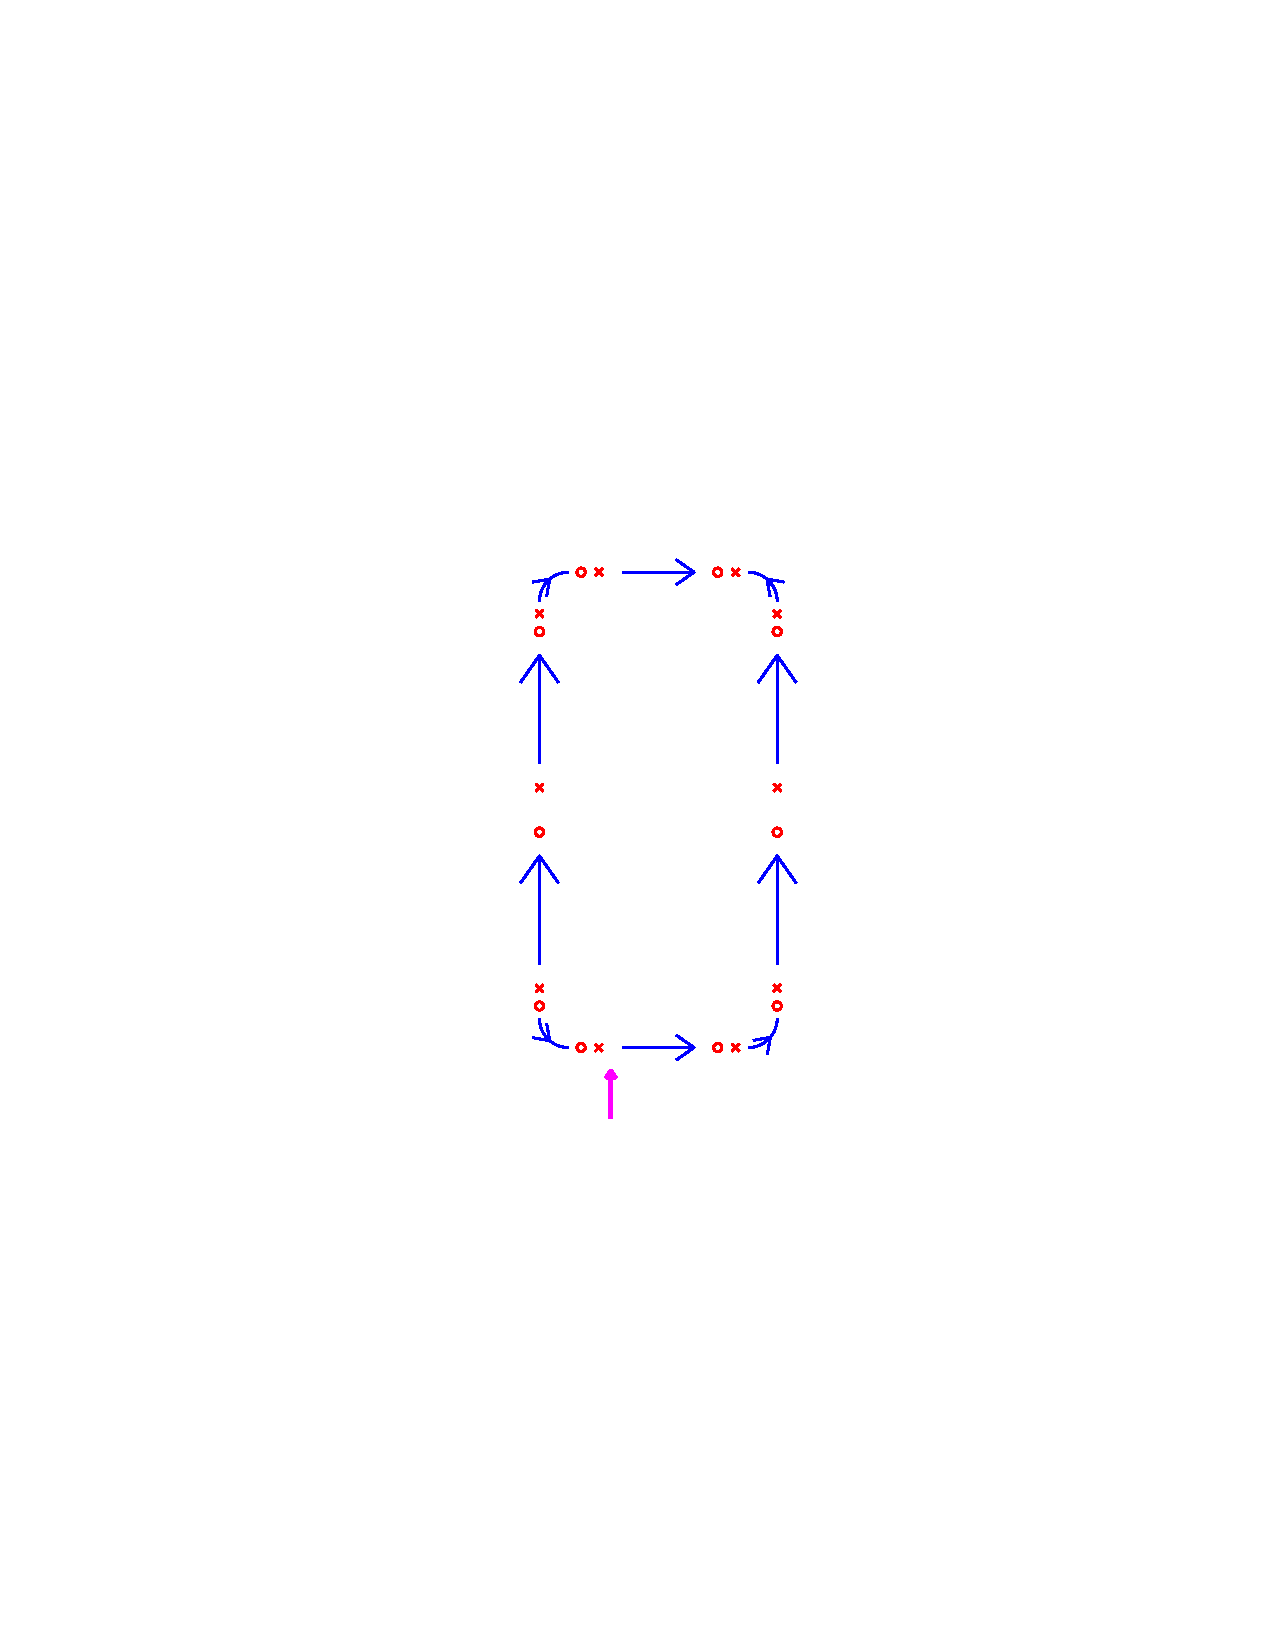
\includegraphics[width=7cm]{example}
\caption{{\it Example.\label{fig:example}}}
\end{center}
\end{figure}
%
We begin the tour with an  arrow of a graph-line, here the point indicated by the magenta arrow. 
Then we move to the right, the signs from the arrow directions are:
$+++++----+$, i.e. the sign of the arrows is $(-)^{4}=+1$. Next we count how often we have the \mode-sequence $xo$, when we move in the direction of the first arrow. There are 5 such 
events. Hence the sign factor is $(-1)^{5}=-1$. The two sign contributions give $-1$, together
with the additional -1 from moving the last variable to the front. The trace
of the product of GV-pairs is $+1$.


Keep in mind, that GV-pairs commute.


\clearpage 

\subsubsection{Basic elements of directed graphs}

In order to determine the weight of connected graph elements it is necessary to take
the direction into account, in which a graph is passed through. Therefore we have to consider directed graphs. Each graph has the  12 basic building blocks. There are 4 straight lines
as shown in figure \ref{fig:lines}, that go right, left, up, or down. 
%
\begin{figure}[h]
\begin{center}
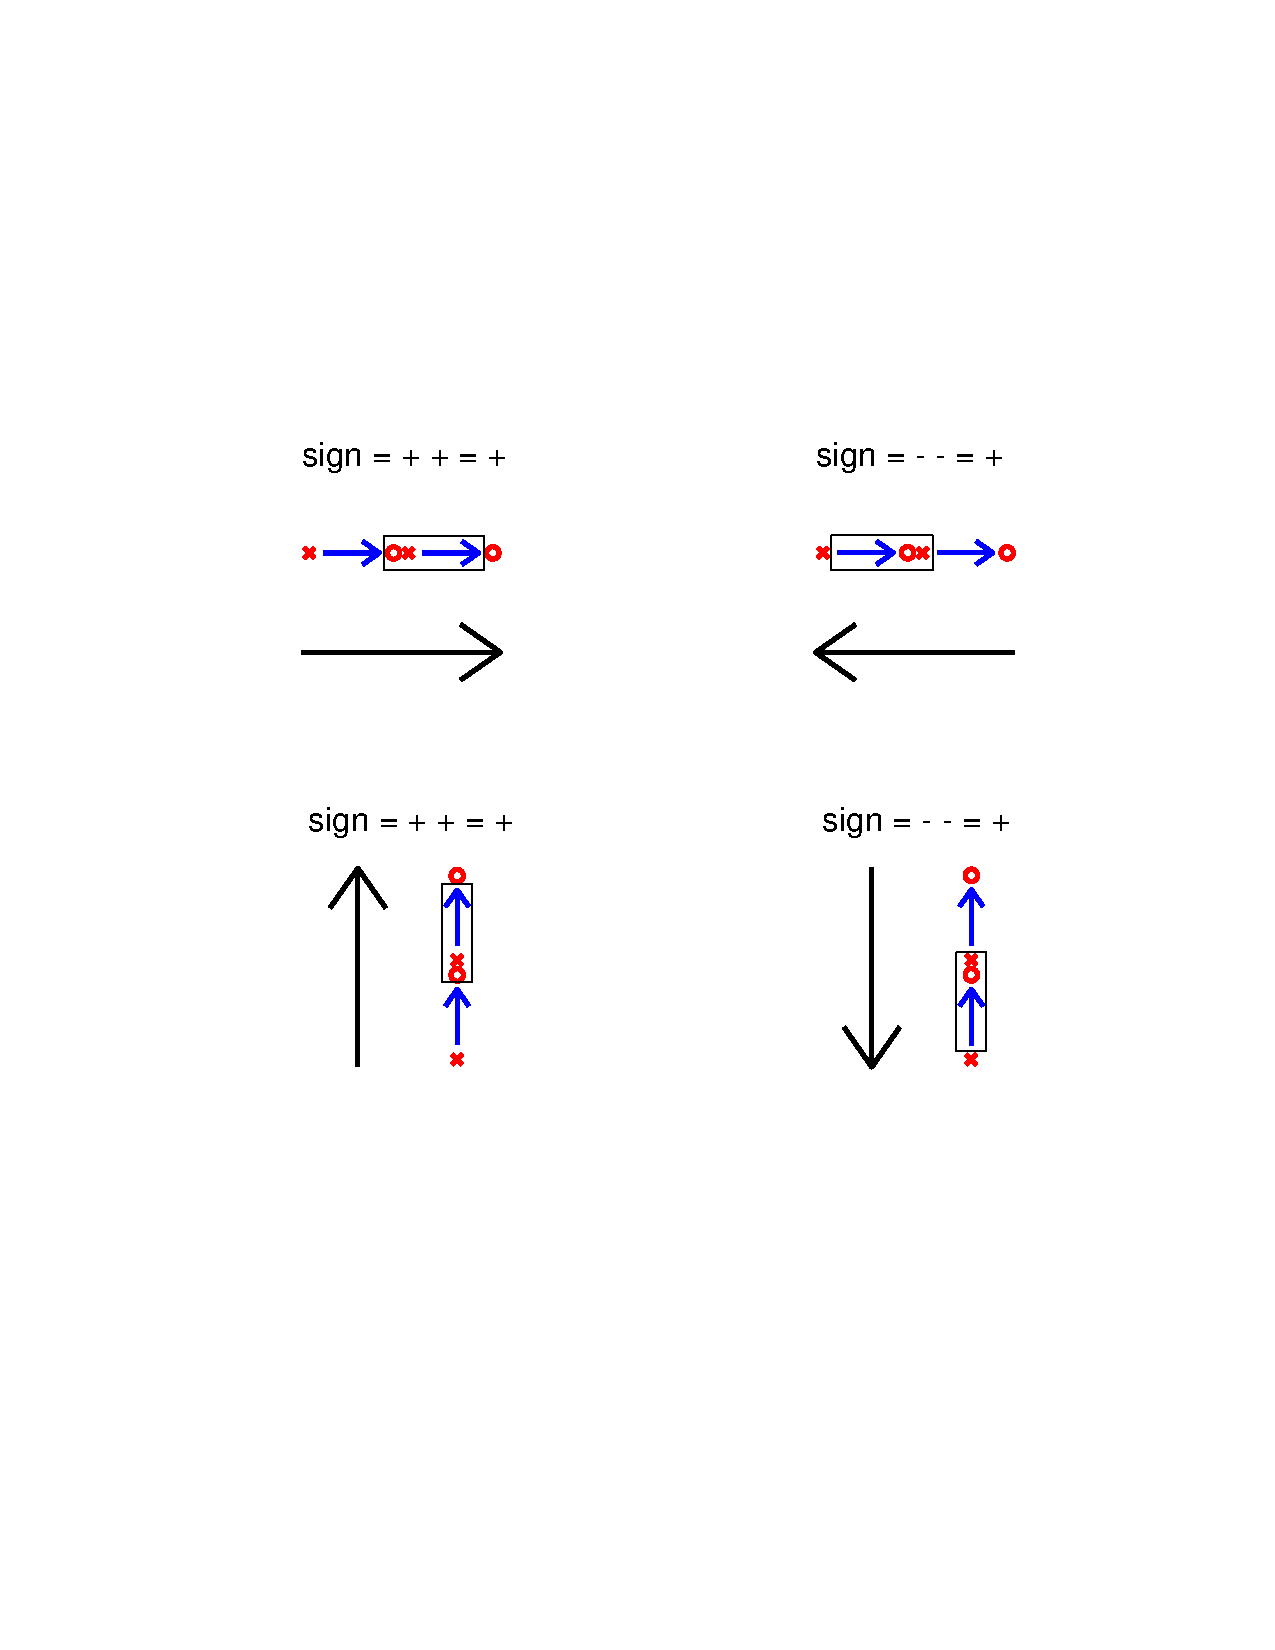
\includegraphics[width=8cm]{lines}
\caption{{\it The 4 different straight paths  and their signs. We see that they all have a positive sign.\label{fig:lines}}}
\end{center}
\end{figure}
%
The actual elements that form these lines are represented in the black boxes. In all cases the sign of the order of the \modes $ox$ and the arrow are the same, resulting in +1 for all 
lines. This is the sign that comes from the trace.

\clearpage
In addition to the lines  there are 8 different corners as depicted in 
figure \ref{fig:directed:graphs}
%
\begin{figure}[h]
\begin{center}
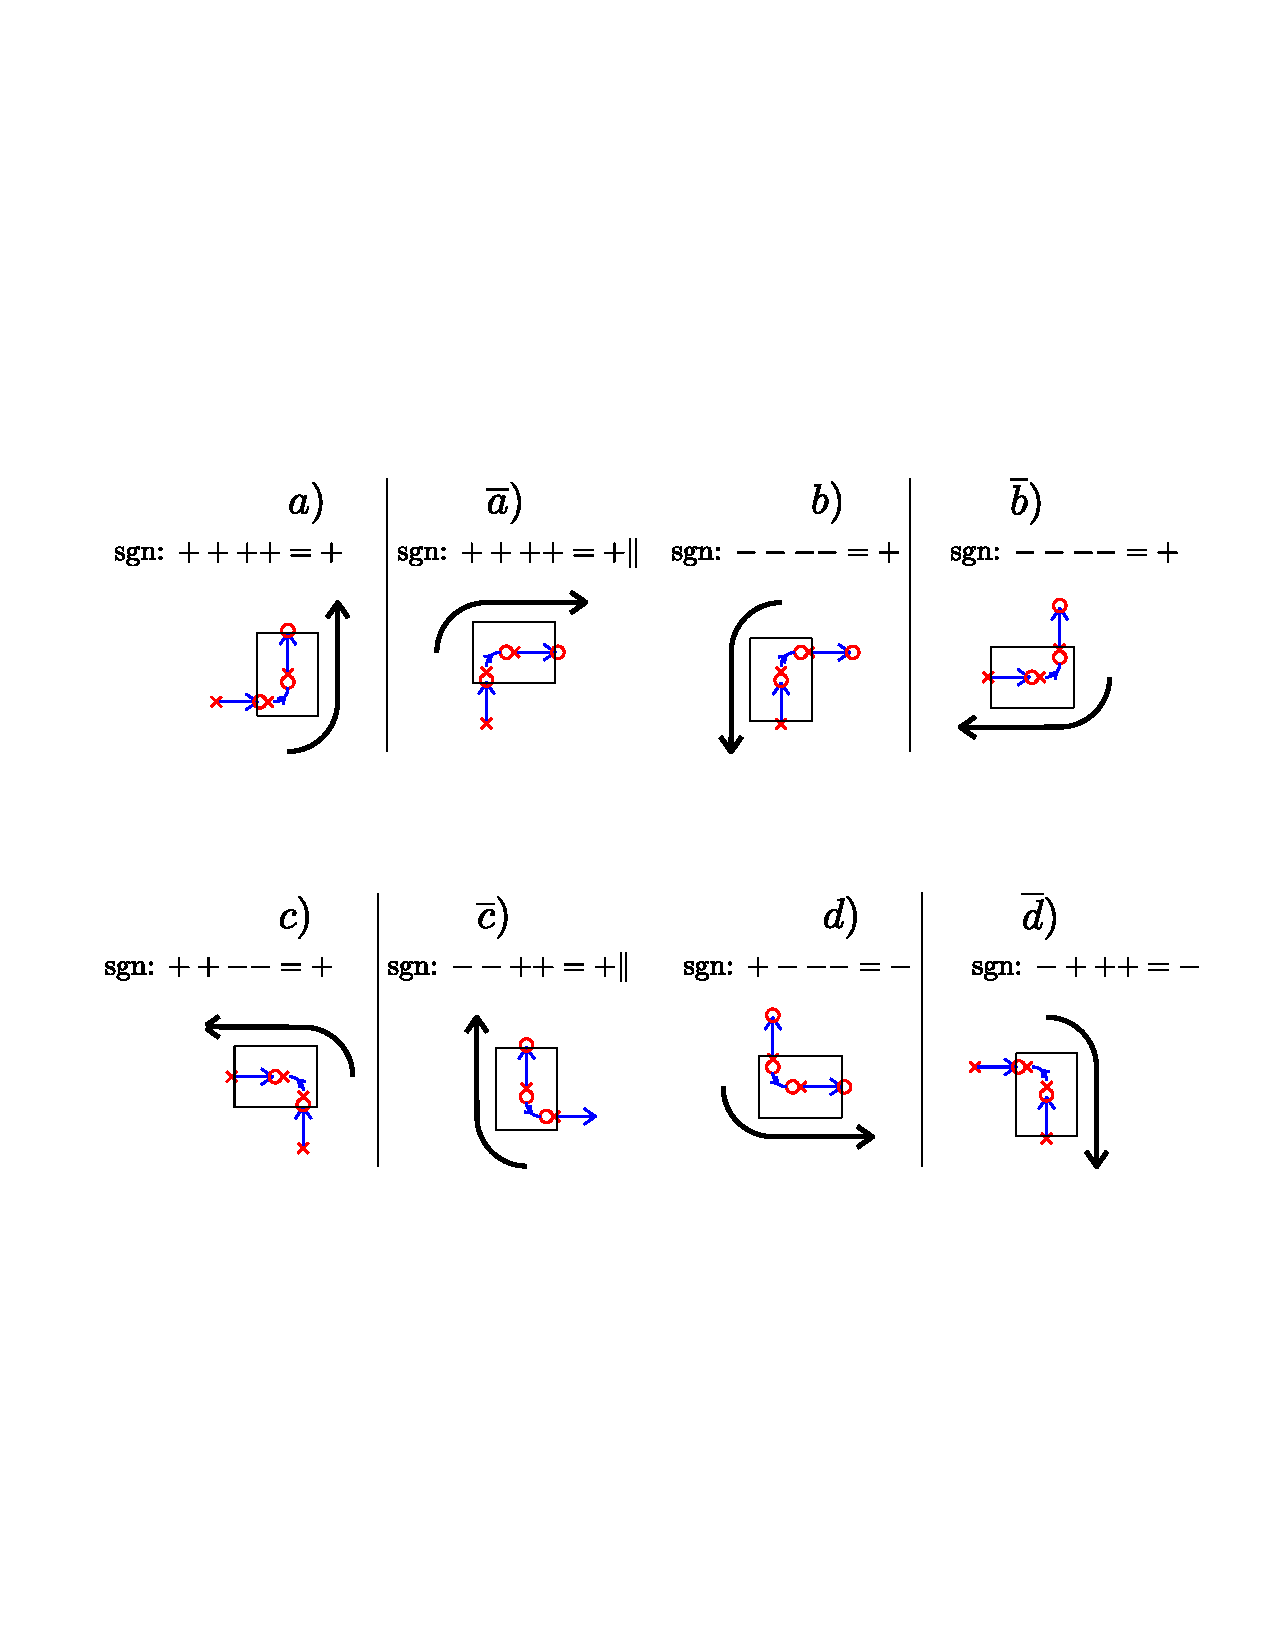
\includegraphics[width=12cm]{corners}
\caption{{\it The 8 different paths around a corner and their signs. The notation is chosen such, that paths $x$ and $\overline x$ start at end at the same connecting points to the rest of the graph, but they are bend in opposite directions.\label{fig:directed:graphs}}}
\end{center}
\end{figure}
%
With these elements we can construct any arbitrary graph  and compute the corresponding weight/ sign. Let us reconsider the example given in figure \ref{fig:example}.
\begin{figure}[h]
\begin{center}
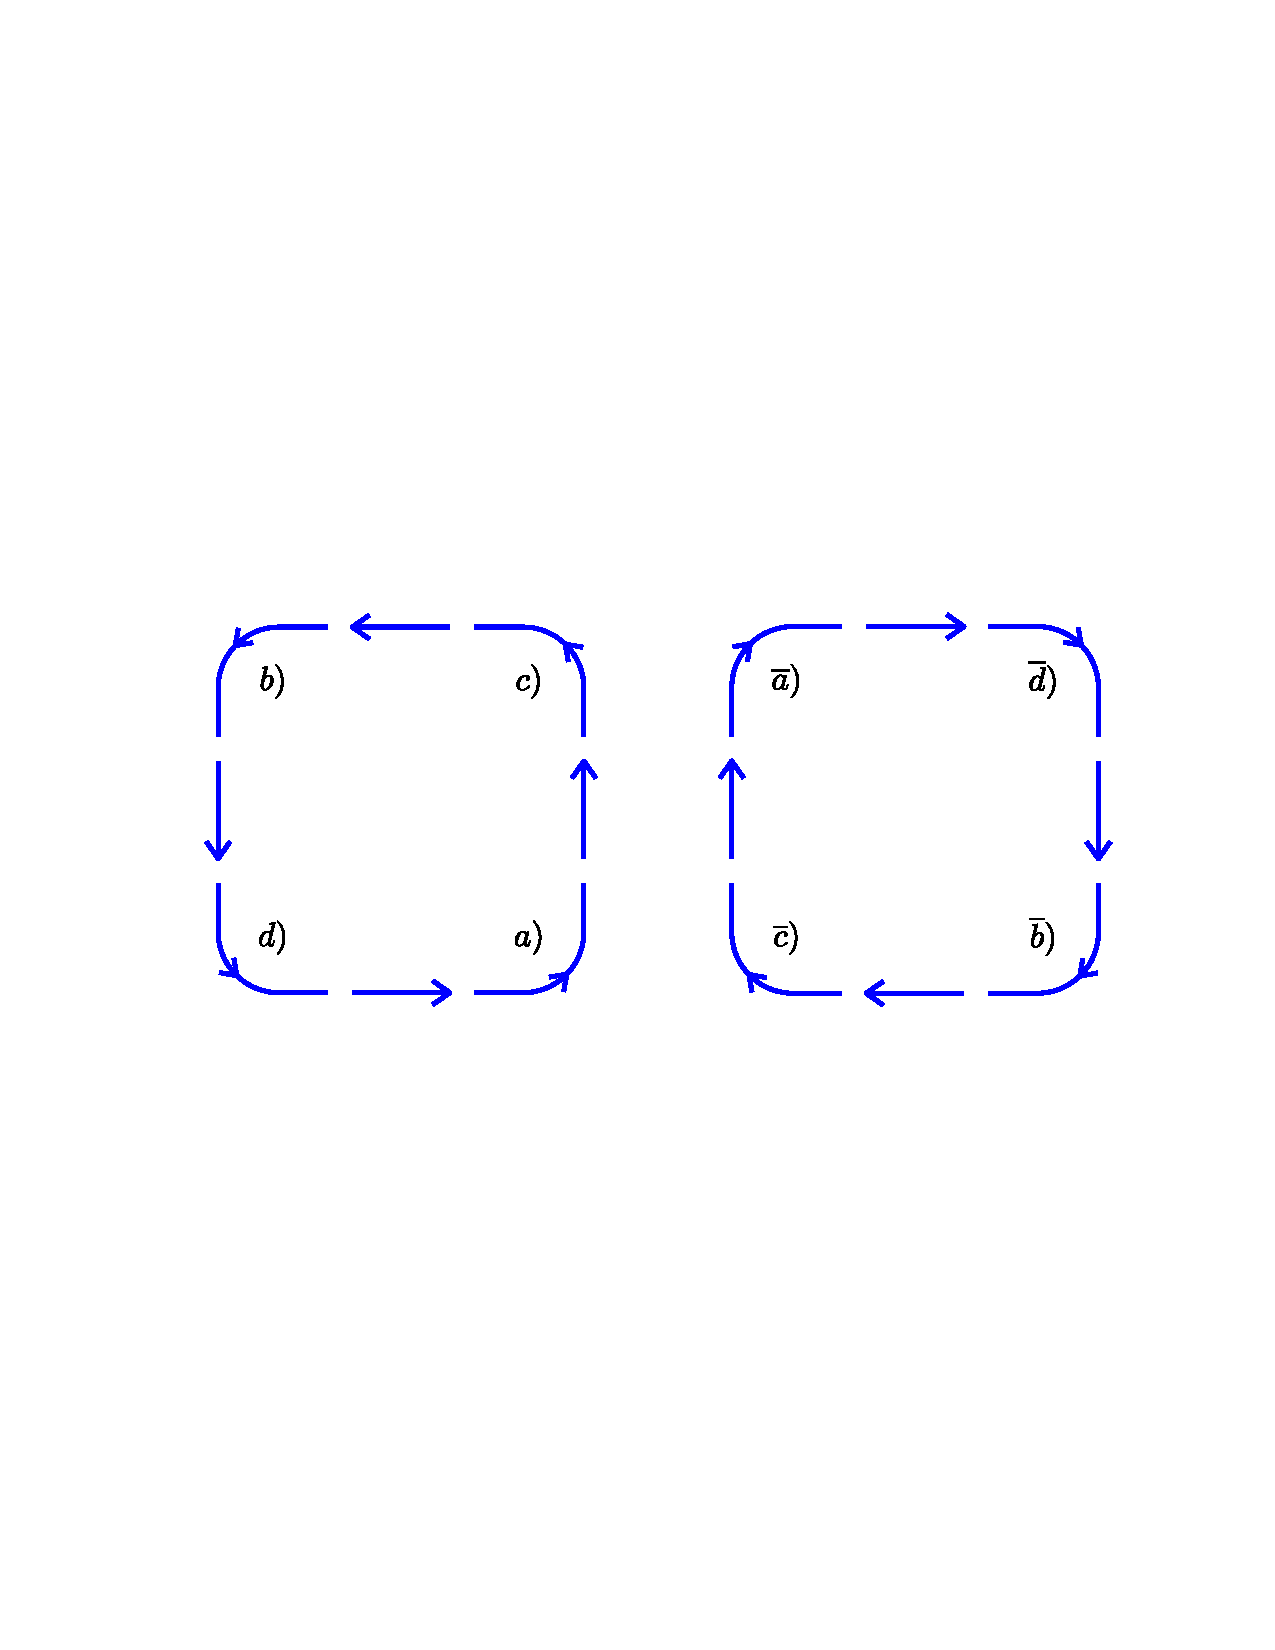
\includegraphics[width=6cm]{example_b}
\caption{{\it Example in directed graphs traversed in different directions.\label{fig:directed:graphs}}}
\end{center}
\end{figure}
%
We find the same sign as before, namely +1: we have one minus sign from corner $d$ or $\overline d$ and one sign from closing the loop. 
Lets now consider a more complex example of  closed non-overlapping loop:
%
\begin{figure}[h]
\begin{center}
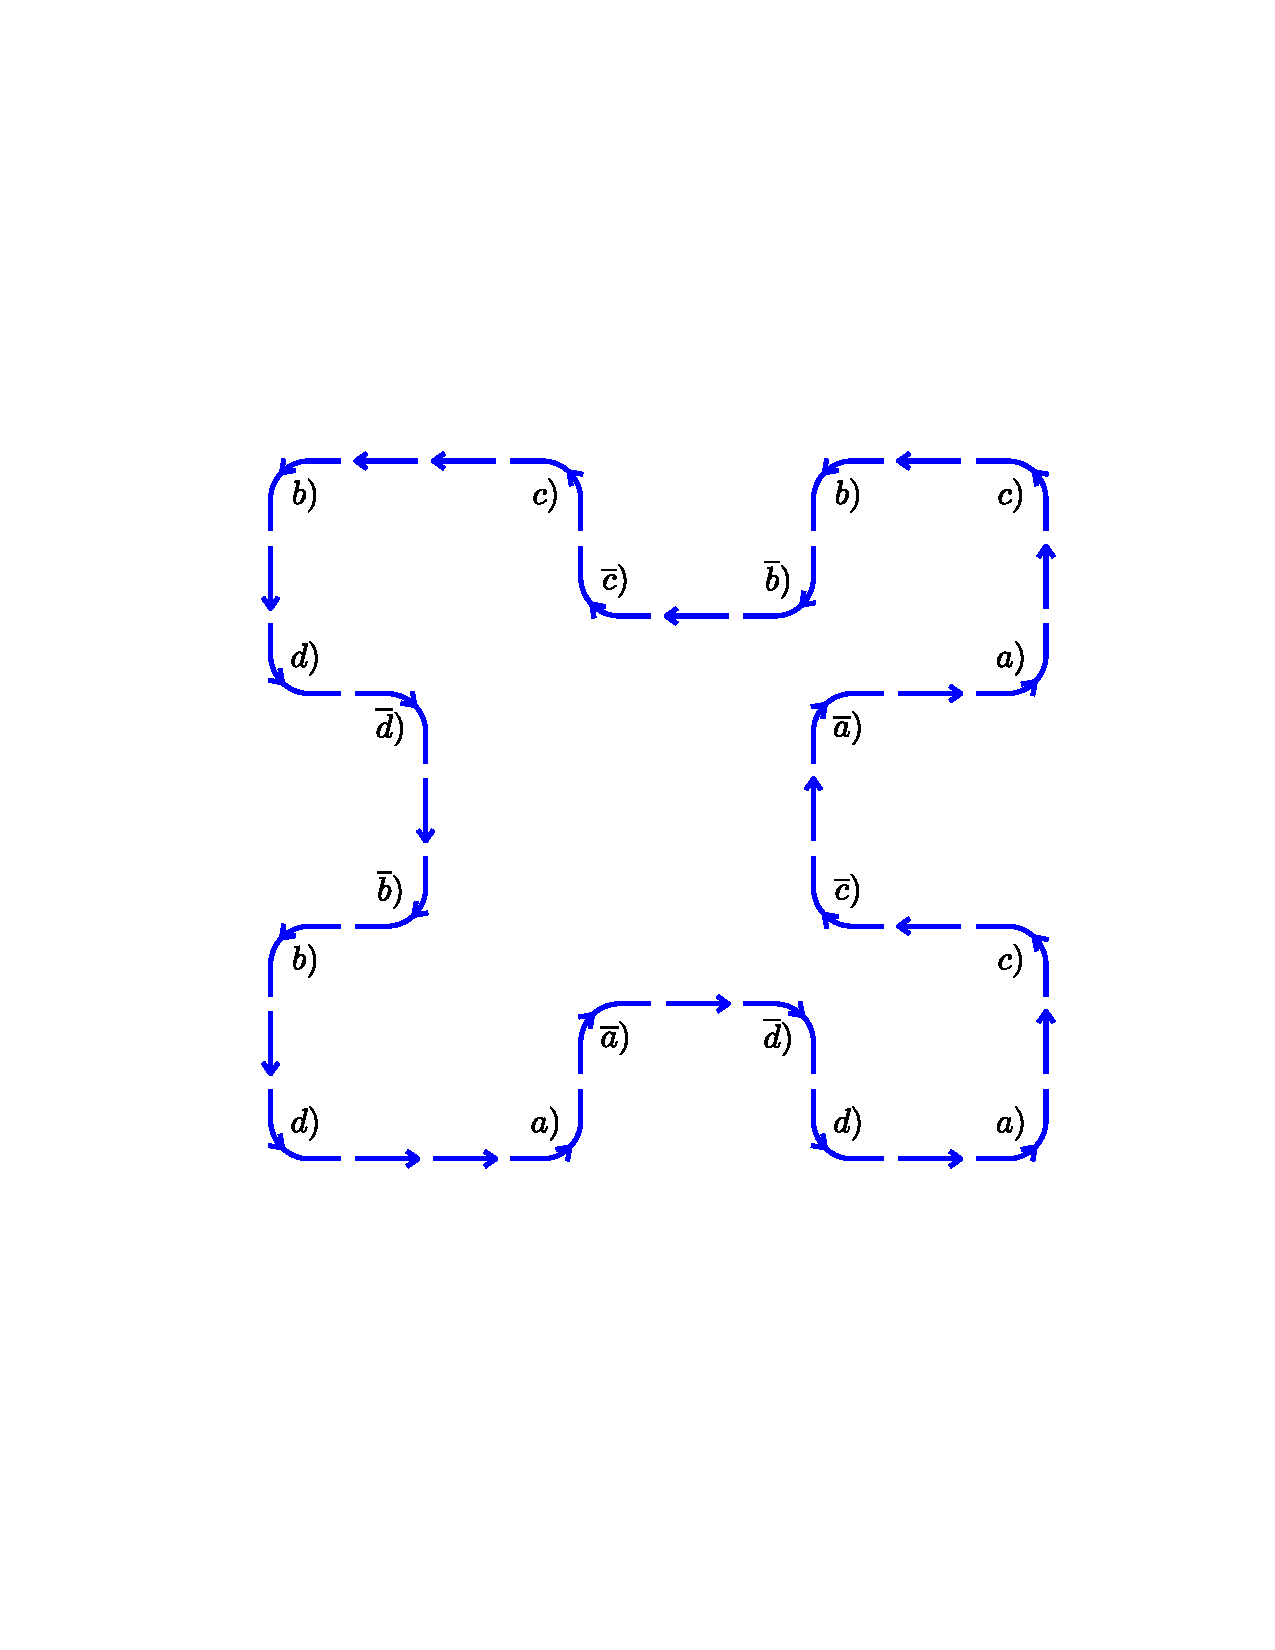
\includegraphics[width=10cm]{example_c}
\caption{{\it More complex example for directed graphs.\label{fig:directed:graphs_more}}}
\end{center}
\end{figure}
%

We can start any closed non-crossing loop  from the simple, square which has a positive sign, and then 
deform it. Each elementary deformation consists of  $x-\overline{x}$-pairs, as can be seen in 
figure \ref{fig:directed:graphs_more}. But the sign of such pairs is always one. Hence,
a closed loops has positive sign


\clearpage

\subsubsection{Impact of the minus sign in the action terms}

To each corner there is associated a minus sign from the action. And also each monomer
required between  lines  passing straight through a site there is also a minus sign. Remember
that the trace over the monomer variables of a sing GV-pair is one. I.e. at each site of a loop we have a minus. Empty sites also have a minus as discussed before. The signs of the action terms does not contribute, since always two terms enter and the sign squared is always on.

We will see  next that also a crossing will yield a minus sign. From the GV-elements we do not get a minus sign






\subsubsection{Sign of crossings}




We consider 2 closed loops, represented by the ellipses connected by a crossing. 
The overall sign is obtained by the signs of the elements in the ellipses, the sign of the crossing and the sign for closing this single connected graph. As before, also polygons with 
crossing are formed by a unique sequence of GV-pairs. And we obtain one extra sign from moving the dangling variable from the end to the beginning (closing sign).
The direction of the path is uniquely given by the arrows. The directions how the crossing is 
passed through, specifies two isolated ellipses. In any case, the directions of the corners
are always pairs of the form $x$ and $\overline x$. 
The total sign of the two separated graph elements (GE) consists of the sign from the elements of the the two 
GE, The sign of the $x$-$\overline x$ pair and two closing sign. 
Corner pairs $x$ / $\overline{x}$  both have the same starting and end point and are bend in opposite directions. On the other hand we know  the sign of the isolates objects already (proof by induction) as $S_{\text{l}_{i}}$. Then we have for the isolated loops
%
\begin{align*}
S_{\text{e}_{1}} * S_{\text{e}_{2}}  *
\underbrace{
S_{x} * S_{\overline x}
}_{\color{blue} = 1} * \underbrace{
S_{\text{closing}}^{2}
}_{\color{blue} = 1}
 &= S_{\text{l}_{1}} * S_{\text{l}_{2}}\\
\Rightarrow\qquad S_{\text{e}_{1}} * S_{\text{e}_{2}}
&= S_{\text{GE}_{1}} * S_{\text{GE}_{2}}\;.
\end{align*}
%
and the overall sign of the connected graph, that has  only one additional crossing is 
%
\begin{align}\label{eq:signrule:crossing}
S_{\text{total}} &= 
S_{\text{e}_{1}} * S_{\text{e}_{2}} * \underbrace{
S_{\text{str.lines}}
}_{\color{blue} = 1} * \underbrace{S_{\text{closing}}}_{\color{blue} = -1} = - S_{\text{GE}_{1}} * S_{\text{GE}_{2}}
\end{align}
%
Of course, the disconnected graph elements have to be shifted apart to obtain an admissible graph, but that has no impact on the sign argument.

Let's begin with a situation, where the separated graph elements are simple loops. Then both have a positive sign. The resulting connected graph with one crossing then has a negative sign.

%We are prompted to claim  that the sign of a connected graph element is $(-1)N_{c}$, where $N_{c}$ is the number of crossings.

We pick out any connected graph  elements with $N_{c}\ge 1$ and separat it at  one of the crossings, such that one of the  resulting separate objects is a loop with zero crossings and the other has therefore $N_{c}-1$ crossings. The sign of a graph element with $N_{c}$ crossings is then according \eq{eq:signrule:crossing}
%
\begin{align*}
S_{N_{c}} &= (-1) * S_{N_{c}-1} * \underbrace{
S_{N_{c}=0}
}_{\color{blue} = 1} = -S_{N_{c}-1}\\
\Rightarrow\qquad S_{N_{c}} &= (-1)^{N_{c}}\;.
\end{align*}
%
Hence each crossing in a graph introduces a minus sign. The origin is the trace. From the
building blocks there is no sign, as they are made of 4 bond GV-pairs, i.e.
they add a factor $t^{4}$, which is accounted for explicitly.

So we have the following situation: An empty site obtains a minus sign and  a site obtaining GV-pairs that from a crossing also have a minus sign, which results in both cases from the trace. The signs in front of the GV-s in the actions is +1 as the GV-pairs occur in pairs
in order to from an empty site or crossing.
This is different at straight lines and corners. At sites, where straight lines pass through,
a monomer is needed. Its contribution to the trace is +1, but it also has a weight factor
$a_{m}$, which now enters individually and not in pairs as in he case of empty sites. Hence
a site with a straight line passing through  gets a factor $a_{m}$. A site with a corner gets in addition to its contribution to the trace a factor $a_{c}$.

Since crossings and empty sites contribute unavoidably a minus sigh to the
corresponding sites, it is necessary to choose $a_{m}=a_{corner}=-1$, to make all sites equal.
Now they all contribute $-1$. Hence, we have to correct the partition function by an overall
factor 
%
\begin{align*}
(-1)^{N}\;,
\end{align*}
%
which in case of an even number of sites vanishes.



\subsection{Boundary Conditions}
We have fond so far that the sign of closed of all graphs is $(-1)^{N}$, i.e. each site contributes a
minus sign. There are several possibilities
\begin{enumerate}
	\item A corner gets a sign from the minus sign in the action for corners
	\item A straight line gets a sign from the minus sign from the corresponding monomer (which is perpendicular to the line)
	\item Empty sites have a minus sign as discussed before
	\item Crossings add a minus sign as discussed before.
\end{enumerate}
Wha we discussed so far is only  concerning the signs is only true for loops that do not close 
across a boundary.
Let's consider e.g. a straight horizontal line that is closed due to periodic boundary conditions across the boundary. Then we have schematically
%
\begin{align*}
&
\int \qty(\prod_{i} d\hdag{i} d\hnag{i})  \red{ \hdag{1}}\hnag{2}\hdag{2}\hnag{3} \cdots \hdag{N-1}\hnag{N}\hdag{N}\hnag{1} \\
&\qquad = 
- \int \qty(\prod_{i} d\hdag{i} d\hnag{i})   \hnag{2}\hdag{2}\hnag{3} \cdots \hdag{N-1}\hnag{N}\hdag{N}\hnag{1} \red{\hdag{1}}\\
&\qquad = 
-\prod_{i} \qty(\underbrace{
\int d\hdag{i} d\hnag{i} \; \hnag{i}\hdag{i}
}_{\color{blue} = 1})\\
&\qquad = - 1
\end{align*}
% 
In addition we have a minus sign on each site of the line from dangling monomer 
as discussed before. In comparison to a straight elements that are not part of a  closed loop across the boundary, there is an extra minus sign.

Unfortunately, the extra sign from the boundary is not simply given by the number of boundary crossings. That could be cured by aperiodic boundary conditions. 
Let's consider one horziontal and one vertical line closed across the boundary.
In that case both line are constructed by independent GV-pairs and the trace is merely the product of the individual traces, which gives $(-1)^{2}=+1$. In this situation, the crossing
does not give an extra minus sign, which it does when it is part of a graph that is not closed
across the boundary.

Hence, we cannot correctly count the graphs required for the Ising model with periodic boundary conditions by Grassmann variables and the action terms introduced so far.
For small $t$ values the impact of terms with winding number greater than one are unimportant, so we could use the Grassmann representation for small values of $t$ but not for the entire
interval $t\in(0,1)$. To avoid the sign problem we instead use open boundary conditions. Then
the graphs are all positively counted.



\subsection{Fourier transform of Grassmann variables} 
%todo Fourier transform GV
Although we are considering open boundary conditions, we still use the Fouriertrasnform
for periodic boundary conditions.
I.e., we  introduce the Fourier transform $\eta^{\alpha}_{\vv k}$ of the  GVs $\eta^{\alpha}_{i}$:
%
\begin{align}\label{eq:FT:GV}
 \eta^{\alpha}_{\vv k} &= \frac{1}{\sqrt{N}} \sum_{i}  \eta^{\alpha}_{i} e^{i \xx{i} \vv k}\\
  \eta^{\alpha}_{\xx{i}} &= \frac{1}{\sqrt{N}} \sum_{\vv k}^{1.b.z.}  \eta^{\alpha}_{\vv k} 
  e^{-i \xx{i} \vv k}\;,
\end{align}
%
with $k_{\alpha} = \frac{2\pi}{L_{\alpha}} n_{\alpha}$ with $n_{\alpha} = 0,1,\ldots L_{\alpha}-1$,
and for the integral
%
\begin{align}\label{eq:}
d \eta^{\alpha}_{\vv k} &= \frac{1}{\sqrt{N}} \sum_{i}  d\eta^{\alpha}_{i} e^{-i \xx{i} \vv k}\\
d  \eta^{\alpha}_{\xx{i}} &= \frac{1}{\sqrt{N}} \sum_{\vv k}^{1.b.z.}  d\eta^{\alpha}_{\vv k} 
  e^{i\xx{i} \vv k}\;.
\end{align}

The Fourier-transformed GVs are also GVs:
%
\begin{align}
 \eta^{\alpha}_{\vv k}  \eta^{\alpha'}_{\vv k'} 
 &= - \eta^{\alpha'}_{\vv k'}  \eta^{\alpha}_{\vv k}  \;,
\end{align}
%
which is seen by inserting the definition and using the anti-commuting properties of the
original GVs.
The FT GVs also have the correct integral properties, that follow from
%

\begin{subequations}
\begin{align}
\int d  \eta^{\alpha}_{\xx{i}} &= 0\label{eq:GV:int:a}\\
\int d  \eta^{\alpha}_{\xx{i}}\eta^{\alpha'}_{\xx{i'}} &= \delta_{\alpha\alpha'}\delta_{ii'}\;.
\label{eq:GV:int:b}
\end{align}
\end{subequations}

%
Then
%
\begin{align*}
\int d  \eta^{\alpha}_{\vv k} &= 0\\
\int d  \eta^{\alpha}_{\vv k} \eta^{\alpha'}_{\vv k'}&= \delta_{\vv k,\vv k'}\delta_{\alpha\alpha'} \;.
\end{align*}
%
The proof of the first property is simply obtained by inserting the definition of the 
FT and using \eq{eq:GV:int:a}. The proof of the second equation is as follows
%
\begin{align*}
\int d  \eta^{\alpha}_{\vv k} \eta^{\alpha'}_{\vv k'}
&=\frac{1}{N}\sum_{i,j} e^{i\big(-\vv k\xx{i} +\vv k'\xx{j}\big)} 
\underbrace{
\int d\eta^{\alpha}_{\xx{i}} \eta^{\alpha'}_{\xx{j}}
}_{\color{blue} = \delta_{i,j}\delta_{\alpha,\alpha'}}\\
&=\frac{1}{N}\sum_{i} e^{i\big(-\vv k +\vv k'\big)\xx{i}}   = \delta_{\vv k,\vv k'}
\end{align*}
%
The FT for the local action terms is simply 
\begin{subequations}\label{eq:}
\begin{align}
A_\text{corners} &=  -\sum_{\vv k} \big(\hdag{\vv k} \vnag{-\vv k}+\vdag{\vv k} \hnag{-\vv k}
+\vdag{\vv k} \hdag{-\vv k} +\vnag{\vv k} \hnag{-\vv k} \big)\\
A_\text{monomers} &=  \sum_{\vv k} \big(\hdag{\vv k} \hnag{-\vv k}
+\vdag{\vv k}\vnag{-\vv k} \big) \;.
\end{align}
\end{subequations}
%
The obc enters in the bond term.
For the treatment of the boundary condition it is best to introduce the  indices for the two directions
%
\begin{align*}
 A^{obc}_\text{bonds}  &= t \sum_{i=1}^{L_{x}-1} \sum_{j=1}^{L_{y}}
 \hdag{i,j} \hnag{i+1,j}
+ t \sum_{i=1}^{L_{x}} \sum_{j=1}^{L_{y}-1} \vdag{i,j} \vnag{i,j+1}\\
&= A^{pbc}  + \Delta A_\text{bonds}\\
\Delta A_\text{bonds} &=- \qty(t  \sum_{j=1}^{L_{y}}
 \hdag{N,j} \hnag{1,j}
+ t \sum_{i=1}^{L_{x}}\vdag{i,N} \vnag{i,1})\;.
\end{align*}
%
Then 
%
\begin{align*}
A^{pbc}_\text{bonds} &= \sum_{\vv k} \big(\varepsilon(k_{x}) \hdag{\vv k} \hnag{-\vv k}
+ \varepsilon(k_{y}) \vdag{\vv k} \vnag{-\vv k}\big)\\
\end{align*}
%
and
%
\begin{align*}
\Delta  A_\text{bonds}  
&=-\frac{t }{L_{x}L_{y}}\sum_{\vv k \vv k'} \hdag{\vv k}\hnag{\vv k'} 
\qty(\underbrace{
e^{- i \qty(k_{x} N + k'_{x} 1)}
}_{\color{blue} = e^{- i k'_{x}}}
\underbrace{
\sum_{j=1}^{L_{y}} e^{-i \qty(k_{y} j +  k'_{y} j)}
}_{\color{blue} = L_{y}\delta_{k'_{y},-k_{y}}})
\\
&\ldots- 
\frac{t }{L_{x}L_{y}}\sum_{\vv k \vv k'} \hdag{\vv k}\hnag{\vv k'} 
\qty(\underbrace{
e^{- i \qty(k_{y} N + k'_{y} 1)}
}_{\color{blue} = e^{- i k'_{y} }}
\underbrace{
\sum_{i=1}^{L_{x}} e^{-i \qty(k_{x} i +  k'_{x} i)}
}_{\color{blue} = L_{x} \delta_{k'_{x},-k_{x}}})\\
&=-\frac{t}{L_{x}} \sum_{k_{y}}\sum_{k_{x}k'_{x}} \hdag{ k_{x}k_{y}}\hnag{k'_{x},-k_{y}} 
e^{- i k'_{x}} -
\frac{t}{L_{y}} \sum_{k_{x}}\sum_{k_{y}k'_{y}}  \hdag{k_{x},k_{y}}\hnag{-k_{x},k'_{y}} 
e^{- i k'_{y} }
\end{align*}
%



 After FT the action reads
 %
\begin{subequations}\label{eq:}
\begin{align}
A &= A_\text{bonds}  + A_\text{corners}  + A_\text{monomers}\\
A_\text{bonds} &= \sum_{\vv k} \big(\varepsilon(k_{x}) \hdag{\vv k} \hnag{-\vv k}
+ \varepsilon(k_{y}) \vdag{\vv k} \vnag{-\vv k}\big)\\
A_\text{corners} &=  -\sum_{\vv k} \big(\hdag{\vv k} \vnag{-\vv k}+\vdag{\vv k} \hnag{-\vv k}
+\vdag{\vv k} \hdag{-\vv k} +\vnag{\vv k} \hnag{-\vv k} \big)\\
A_\text{monomers} &=  \sum_{\vv k} \big(\hdag{\vv k} \hnag{-\vv k}
+\vdag{\vv k}\vnag{-\vv k} \big) \;.
\end{align}
\end{subequations}
%
We can combine the bonds and the monomers to 

%
\begin{align*}
A_\text{bpm} &= \sum_{\vv k} \big(\tilde \varepsilon(k_{x}) \hdag{\vv k} \hnag{-\vv k}
+ \tilde \varepsilon(k_{y}) \vdag{\vv k} \vnag{-\vv k}\big)\\
\tilde \varepsilon(k) &= 1+\varepsilon(k)
=1 + t e^{i k} \;.
\end{align*}
%
In the sum we omit the term $\vv k=0$, as it has a vanishing contribution in the thermodynamic limit.
Next we use the ordering of the 
We can also use the GV-properties to symmetries the action by adding the term where the pair of GVs are swapped and $\vv k \to -\vv k$.
%
\begin{align*}
A &= A_\text{bpm}  + A_\text{corners}\\
A_\text{bpm} &=\frac{1}{2}\sum_{\vv k} \big(\tilde \varepsilon(k_{x}) \hdag{\vv k} \hnag{-\vv k}
-\tilde \varepsilon(-k_{x}) \hnag{\vv k} \hdag{-\vv k} 
+ \tilde \varepsilon(k_{y}) \vdag{\vv k} \vnag{-\vv k}
- \tilde \varepsilon(k_{y}) \vnag{\vv k} \vdag{-\vv k} 
\big)\\
A_\text{corners} &=  -\frac{1}{2}\sum_{\vv k} \big(
\hdag{\vv k} \vnag{-\vv k}
-\vnag{\vv k} \hdag{-\vv k} 
+\vdag{\vv k} \hnag{-\vv k}
- \hnag{\vv k}\vdag{-\vv k}\\
&\qquad\qquad     \ldots 
+\vdag{\vv k} \hdag{-\vv k} 
-\hdag{\vv k}  \vdag{-\vv k} 
+\vnag{\vv k} \hnag{-\vv k} 
- \hnag{\vv k} \vnag{-\vv k}\big)
\end{align*}
% 
We combine all GVs that belong to the same $\vv k$ into a vector.%
\begin{align*}
\vv \eta_{k} &= \big( \hdag{\vv k}, \hnag{\vv k}, \vdag{\vv k}, \vnag{\vv k}\big)^{T}
\end{align*}
%
Then the action can be written as
%
\begin{align*}
A &=  \frac{1}{2}\sum_{\vv k} \vv \eta_{\vv k}^{T}  M_{\vv k}  \eta_{-\vv k}
 =  \sum'_{\vv k} \vv \eta_{\vv k}^{T}  M_{\vv k}  \eta_{-\vv k}\;.\\
\text{with}\quad M_{\vv k} &=
\begin{pmatrix}
&h^{x}& h^{o}& v^{x} & v^{o}\\
\hline
h^{x}|&	0 & \tilde \varepsilon(k_{x}) & 1 & -1\\
h^{o}|&	-\tilde \varepsilon(-k_{x}) & 0  & 1 & 1\\
v^{x}|&	-1 & -1 & 0 & \tilde \varepsilon(k_{y})\\
v^{o}|&	1 & -1 & -\tilde \varepsilon(-k_{y}) & 0
\end{pmatrix}
\end{align*}
%
Here $M$ is an anti-Hermitian  matrix. The symbol $\sum'_{\vv k}$ indicates that $\vv k $ are only taken from the half plane $k_{y} > 0$ or $k_{y}=0$, if $k_{x > 0}$. The second half of the wave vectors is then given uniquely by $-\vv k$.
Moreover, the symbol $\sum'$
also excludes  $\vv k =0$, which has no impact in the thermodynamic limit. 

The Jakobi determinant of the transformation of the measure form real space to momentum space is +1, as outlined in appendix ??.

Then the vectors $\vv\eta_{\vv k} $
$\vv\eta_{-\vv k} $ contain independent GVs. Therefore, the trace gives
%
\begin{align*}
\tr{e^{A}} &= \prod'_{\vv k} \tr{e^{\sum_{\vv k} \vv \eta_{\vv k}^{T}  M_{\vv k}  \eta_{-\vv k}}}
=\prod_{\vv k}' \det\big( M_{\vv k} \big)\;.
\end{align*}
%
The determinant of $M_{\vv k}$ yields
%
\begin{align*}
\det\big( M_{\vv k} \big) &= \big( 1+t^{2} \big)^{2} - 2 t \big(1-t^{2}\big) \big( \cos(k_{x})
+\cos(k_{y}) \big)\;,
\end{align*}
%
which has the symmetry $\det\big( M_{-\vv k} \big) = \det\big( M_{\vv k} \big)$. So we can 
also include the second half plane in k-space in the product and also the term $\vv k=0$ as it 
has vanishing weight in the thermodynamic limit.
Finally, we have 

%
\begin{align}\label{eq:}
Z &= 2^{N} \cosh^{2N}(j) \prod_{\vv k}^{1.B.z.} \bigg( \big( 1+t^{2} \big)^{2} - 2 t \big(1-t^{2}\big) \big( \cos(k_{x})
+\cos(k_{y}) \big)\bigg)^{\frac{1}{2}}\;,
\end{align}
%
which is the Onsager result.


\section{Grassmann algebra}


An n-dimensional Grassmann algebra is the algebra generated by a set of (Grassmann) variables $\{\eta_{i}\}_{i=1:n}$,  satisfying
%
\begin{align}\label{eq:}
\{\eta_{i},\eta_{j}\}=0,  
\end{align}
%
i.e. they anti-commute, which implies in particular that $\eta_{i}^{2} = 0$. The algebra generated by these variables contains all expressions of the form
%
\begin{align*}
f(\eta) &= f_{0} + \sum_{i=1}^{n} f_{i} \eta_{i} + \sum_{i< j} f_{ij} \eta_{i} \eta_{j}
+\sum_{i< j<k} f_{ijk} \eta_{i} \eta_{j} \eta_{k} +\ldots + f_{1\ldots n}\; \eta_{1} \eta_{2} \ldots \eta_{n}\;. \;,
\end{align*}
%
with $f_{\bullet}\in \mathbb{C}$.
Obviously, the highest order term is 
%
\begin{align*}
f_{1\ldots n}\; \eta_{1} \eta_{2} \ldots \eta_{n}\;.
\end{align*}
%
since higher order terms would contain GVs in higher order which is zero.
%
We now define a left derivative $\partial_{i} := \partial_{a_{i}}$ . 
The derivative gives zero on a monomial which does not contain the variable $a_{i}$. 
If the monomial does contain $a_{i}$, it is moved to the left (with the appropriate sign due to the exchanges) and then suppressed. 
The operation is extended by linearity to any element of the algebra. 
A right derivative can be defined similarly. 
From this definition the following rules can be obtained
%
\begin{align*}
\{\partial_{a_{i}}, a_{j}\} &= \delta_{ij}\\
\{\partial_{a_{i}}, \partial_{a_{j}}\} &= 0\;.
\end{align*}
%
Integrals are defined as linear operations over the functions f with the property that they 
can be identified with the (left) derivatives. Correspondingly,
%
%
\begin{align}\label{eq:}
\int da_{i} f(a) &= \partial_{ a_{i}} f(a)\;.
\end{align}
%
Hence,
%
\begin{align*}
\int da_{i}  &= 0\\
\int da_{i} a_{j} &= \delta_{ij}\;.
\end{align*}
%
We also introduce a second set of GVs $\{\psi\}_{i=1:n}$ with the additional propetry
%
\begin{align*}
\{\psi_{i},\eta_{j}\} &= 0\;,\qquad \forall i,j\;.
\end{align*}
%
Next we compute exponentials of the form

%
\begin{align}\label{eq:gaussian:A}
\int\ldots\int \Dep e^{\vv\psi^{T} A \;\vv \eta} &=
\int\ldots\int \Dep\; e^{\frac{1}{2} \sum_{ij} \psi_{i} A_{ij} \eta_{j}}\\
&=\int\ldots\int \Dep \;\prod_{i<j} e^{A_{ij} \eta_{i}\eta_{j} }\\
&=\int\ldots\int \Dep \;\prod_{i<j} \underbrace{
\big(1 + A_{ij} \eta_{i}\eta_{j}\big)
}_{\color{blue} = B_{ij}}\;.
\end{align}
%
The Grassmann-measure is defined as
%
\begin{align*}
\Dep &:= \prod_{i} d \eta_{i} d\psi_{i}\;.
\end{align*}
%
Hence
%
\begin{align}\label{eq:fundamental:integral}
\int\ldots\int \Dep \prod_{i} \psi_{i} \eta_{i}&= 1\;.
\end{align}
%

We continue with \eq{eq:gaussian:A}
The double product can be formally written as
%
\begin{align}\label{eq:square:bracket}
\prod_{ij} B_{ij} &= \bigg[B_{11}\ldots B_{1n}\bigg]\times  \bigg[B_{21}\ldots B_{2n} \bigg]\times \ldots \times 
\bigg[ B_{n1}\ldots B_{nn}\bigg]
\end{align}
%
There are $2^{n^{2}}$ possible terms, by choosing  the 1 or the term $A_{ij}\psi_{i}\eta_{j}$ from each $B_{ij}$-term.
However, most of these combinations result in a vanishing trace because some of the GVs occur several times or not at all. The only choices that give a non vanishing contribution to the trace are as follows: From 
each  square bracket in \eq{eq:square:bracket}  choose one and only one $A_{i j} \psi_{i}\eta_{j}$ and the other terms contribute  1. 
The contribution of the $l$-th square brackets is
$A_{l,j_{l}} \psi_{l}\eta_{j_{l}}$.
Thus, each $\psi_{i}$ occurs precisely once. To ensure that this is also true for the $\eta_{j}$,
the set of indices  $\{j_{l}\}$ can only be permutations of the indices $\{1,2,\ldots,n\}$, which 
leads to
%
\begin{align}\label{eq:gaussian:B}
\int\ldots\int \Dep\; e^{\vv\psi^{T} A \;\vv \eta} &=
\sum_{\cP } \bigg(\prod_{l=1}^{n} A_{l,\cP _{l}}\bigg)\;\int\ldots\int \Dep 
\bigg( \prod_{l=l}^{n}\psi_{l} \eta_{\cP _{l}}  \bigg)\;.
\end{align}
%
Finally, we need to bring the permuted indices back into the natural order. To this end, we first
move the $\eta_{j}$ GVs to the very end, by retaining there mutual order, i.e.
\begin{align*}
\prod_{l}\psi_{l} \;\eta_{\cP _{l}}&= 
\text{sign} \cdot \prod_{l}\psi_{l} \;\prod_{l}\eta_{\cP _{l}}
\end{align*}
%
Here, $\text{sign}$ is the sign associated with separating the $\eta$- from the $\psi$-variables.
Next we bring the $\eta$-s into their natural order
\begin{align*}
\prod_{l}\psi_{l} \;\eta_{\cP _{l}}&= \text{sign} \big( \cP  \big)\cdot
\text{sign} \cdot \prod_{l}\psi_{l} \;\prod_{l}\eta_{l}
\end{align*}
%
Eventually, we form again the $\eta-\psi$-pairs, which again introduces the same sign as in the first step:
%
\begin{align*}
\prod_{l}\psi_{l} \;\eta_{\cP _{l}}&= \text{sign}\big( \cP  \big)
\big(\text{sign}\big)^{2} \prod_{l}\psi_{l} \eta_{l}\\
&=\text{sign}\big( \cP  \big)\prod_{l}\psi_{l} \eta_{l}
\end{align*}
%
Along with \eq{eq:fundamental:integral} and \eq{eq:gaussian:B}, we have
%
\begin{align*}
\int\ldots\int \Dep\; e^{\vv\psi^{T} A \;\vv \eta} &=
\sum_{\cP }\text{sign}\big( \cP  \big)\; \bigg(\prod_{l=1}^{n} A_{l,\cP _{l}}\bigg)\;.
\end{align*}
%
and finally
%
\tboxitp{Gaussian integral}{of type I}{
\begin{align}\label{eq:gaussian:C}
\int\ldots\int \Dep\; e^{\vv\psi^{T} A \;\vv \eta} 
&=\det\big( A \big)\;.
\end{align}}

\subsubsection{Gaussian integral II}




In this section we compute exponentials of the form
%
\begin{align}\label{eq:gaussian:II:A}
\int\ldots\int \Deta  e^{\frac{1}{2}\vv\eta^{T} A \;\vv \eta} &=
\int\ldots\int \Deta\; e^{\frac{1}{2}\sum_{ij} \eta_{i} A_{ij} \eta_{j}}\;.
\end{align}
%
The Grassmann-measure is defined now as
%
\begin{align*}
\Deta  &:= d \eta_{n} d \eta_{n-1} \ldots d \eta_{1}\;.
\end{align*}
%
In this case $A$ has to be anti-Hermitian/ skew-symmetric , i.e. 
%
\begin{align*}
A_{ji} &= - A_{ij}\\
\text{then}\quad \frac{1}{2}\sum_{ij} \eta_{i} A_{ij} \eta_{j} &=
\sum_{i<j} \eta_{i} A_{ij} \eta_{j}\;.
\end{align*}
%
We consider only the case of even dimension $n=2 m$.
Then
%
\begin{align}\label{eq:gaussian:II:B}
\int\ldots\int \Deta  e^{\frac{1}{2}\vv\eta^{T} A \;\vv \eta}
&=\int\ldots\int \Deta  \;\prod_{i<j} e^{A_{ij} \eta_{i}\eta_{j} }\\
&=\int\ldots\int \Deta \;\prod_{i<j} \underbrace{
\big(1 + A_{ij} \eta_{i}\eta_{j}\big)
}_{\color{blue} = B_{ij}}\\
\prod_{i<j} B_{ij} &= \bigg[B_{11}\ldots B_{1n}\bigg]\times  \bigg[B_{23}\ldots B_{2n} \bigg]\times \ldots \times \label{eq:Bs}
\end{align}
%
Each $B_{ij}$ contributes either $1$ of $\kappa_{ij}:=A_{ij}\eta_{i}\eta_{j}$. The product 
splits into a sum of $2^{n*n}$ terms $\{T_{i}\}_{i=1:n*n}$.
But a   a non-vanishing  trace is only obtained if each GV occurs precisely once.
This means that non vanishing terms $T_{i}$ contain  $(n/2=m)$ $\kappa_{ij}$-terms, with
no indices in common, or rather: each index from the list $\{1,2,\ldots,n\}$ occurs once.
The $\kappa_{ij}$ terms describe a pairing between indices $i$ and $j$, with $i<j$.
The non-vanishing combinations $\kappa_{ij}$ terms therefore describes a
partitioning of the set $\{1,2,\ldots,2m\}$ into pairs,
described by 
%
\begin{align*}
\kappa_{i_{1},j_{1}},\kappa_{i_{2},j_{2}},\ldots,\kappa_{i_{m},j_{m}}\;.
\end{align*}
%
Moreover, according to \eq{eq:Bs}, we have 
%
\begin{align*}
i_{l}&< j_{l}\\
i_{1}&<i_{2}<i_{3}\ldots\\
j_{1}&<j_{2}<j_{3}\ldots\,.
\end{align*}
%
Clearly, in the set of $T_{i}$-s all possible pairings occur once and only once. 
%
The set of all such pairings be denote by $P$. An element $\alpha\in P$ is characterised by
%
\begin{align*}
\alpha &= \{(i^{\alpha}_{1},j^{\alpha}_{1}),(i^{\alpha}_{2},j^{\alpha}_{2}),\ldots,(i^{\alpha}_{m},j^{\alpha}_{m})\}\;.
\end{align*}
%
$P$ has $(2m-1)!!$ elements. According to the construction for the non-vanishing trace elements,
we have $i^{\alpha}_{1}< i^{\alpha}_{2}<\ldots < i^{\alpha}_{m}$  and $i^{\alpha}_{l}< j^{\alpha}_{l}$. The contribution of such a partitioning to the trace is
%
\begin{align*}
\prod_{l} A_{i^{\alpha}_{l},j^{\alpha}_{l}} \cdot \int\ldots\int \Deta \;\prod_{l} \eta_{i^{\alpha}_{l}}\eta_{j^{\alpha}_{l}}\;.,
\end{align*}
%
Let $\cP (\alpha)$ be the permutation required to transform 
the sequence $i^{\alpha}_{1},j^{\alpha}_{1},i^{\alpha}_{2},j^{\alpha}_{2},\ldots,i^{\alpha}_{m},j^{\alpha}_{m}$ into the natural  sequence $1,2,\ldots,2m$ , then
%
\begin{align*}
\prod_{l} A_{i^{\alpha}_{l},j^{\alpha}_{l}} \cdot \int\ldots\int \Deta \;\prod_{l} \eta_{i^{\alpha}_{l}}\eta_{j^{\alpha}_{l}} &=\text{sign} (\cP (\alpha))\cdot 
\prod_{l} A_{i^{\alpha}_{l},j^{\alpha}_{l}}  \cdot \underbrace{
\int\ldots\int \Deta \;\prod_{i} \eta_{i}
}_{\color{blue} = 1}\;.
\end{align*}
%
Hence we have
\begin{align}\label{eq:gaussian:II:C}
\int\ldots\int \Deta  e^{\frac{1}{2}\vv\eta^{T} A \;\vv \eta}
&= \sum_{\alpha\in P}  
\text{sign} (\cP (\alpha))\;
\prod_{l=1}^{m} A_{i^{\alpha}_{l},j^{\alpha}_{l}} = \Pf{A})\;.
\end{align}
This is the definition of the Pfaffian. For $n=2m$ the Pfaffian is related to the determinant
via
%
\begin{align*}
\big(\Pf{A}\big)^{2} &= \det(A)
\end{align*}
%

For the proof we use
%
\begin{align*}
A &= U D U^{T}\\
D &=
\begin{pmatrix}
	0&\lambda_{1}&\ldots\\
	-\lambda_{1}&0&\ldots\\
	.&.&	0&\lambda_{2}&\ldots\\
	.&.&	-\lambda_{2}&0&\ldots\
\end{pmatrix}
\end{align*}
%
where $U$ is unitary. We use also
%
\begin{align}\label{eq:eta:xi}
\vv \eta = U \vv \xi\;,
\end{align}
%
and obtain
%
\begin{align*}
\frac{1}{2} \vv\eta^{T} A \vv \eta 
&= \frac{1}{2}\vv \xi^{T} D  \vv \xi\\
&= \sum_{\nu=1}^{m}  \lambda_{\nu} \xi_{2\nu-1}\xi_{2\nu}
\end{align*}
%
Then 
%
\begin{align*}
\int\ldots\int \Deta  e^{\frac{1}{2}\vv\eta^{T} A \;\vv \eta} 
&=\det\big( U \big) \int\ldots\int \Dxi   \prod_{\nu=1}^{m}
e^{\lambda_{\nu} \xi_{2\nu-1}\xi_{2\nu}} \\
&= \det\big( U \big)\prod_{\nu=1}^{m}  \int\int d \xi_{2\nu} d_{2\nu-1}
e^{\lambda_{\nu} \xi_{2\nu-1}\xi_{2\nu}} \\
&= \det\big( U \big)\prod_{\nu=1}^{m}  \underbrace{
\int\int d \xi_{2\nu} d_{2\nu-1}
\big(1+\lambda_{\nu} \xi_{2\nu-1}\xi_{2\nu}\big)
}_{\color{blue} = \lambda_{\nu}} \\
&= \det\big( U \big)\prod_{\nu=1}^{m} \lambda_{\nu} \;.
\end{align*}
%
Next we compute the determinant of $A$
%
\begin{align*}
\det\big( A \big) &=\det\big( U D U^{T} \big) =
\underbrace{
\big(\det(U)\big)^{2}
}_{\color{blue} = 1} \det(D)\\
&=
\det
\begin{pmatrix}
	0&\lambda_{1}&\ldots\\
	-\lambda_{1}&0&\ldots\\
	.&.&	0&\lambda_{2}&\ldots\\
	.&.&	-\lambda_{2}&0&\ldots\
\end{pmatrix}\\
&=
\prod_{\nu=1}^{m}
\det
\begin{pmatrix}
	0&\lambda_{\nu}\\
	-\lambda_{\nu}&0
\end{pmatrix}\\
&=\prod_{\nu=1}^{m} \lambda_{\nu}^{2}\\
&=\bigg(\prod_{\nu=1}^{m} \lambda_{\nu}\bigg)^{2}\\
&=\Pf{A}
\end{align*}
%


\subsubsection{Linear transformations}

We perform a linear transformation on a set of $n$ GVs $\{\eta\}_{i=1:n}$
%
\begin{align}
\eta_{i} &= A_{ij} \xi_{j};.
\end{align}
%
The anti commutator is
%
\begin{align*}
\{\eta_{i},\eta_{i'}\} &=A_{ij} A_{i'j'} \underbrace{
\{ \xi_{j},\xi_{j'}\} 
}_{\color{blue} = 0} = 0\;.
\end{align*}
%
For the differential  we need 
%
\begin{align*}
\partial_{\eta_{i}} \eta_{i'} &= \delta_{ii'}
\end{align*}
%
We expect that the differential $\partial_{\eta_{i}}$ will also be a linear function 
%
\begin{align*}
\partial_{\eta_{i}}ta &= B_{ij} \partial_{\xi_{j}}
\end{align*}
%
with the above constraint leading to
%
\begin{align*}
B_{ij}  A_{i'j'} 
\underbrace{
\partial_{\eta_{j}} \eta_{j'} 
}_{\color{blue} = \delta_{jj'}}
&= \delta_{ii'}\\
\big(B  A^{T} \big)_{ii'} &=  \delta_{ii'}\\
B A^{T} &= \uu\;.
\end{align*}
So we have
%
\begin{align}\label{eq:B:A}
B &= \big(A^{-1}\big)^{T}\;.
\end{align}
%
Especially for unitary transformations ($A^{-1}=A^{\dagger}$) we have
%
\begin{align*}
B &= \big(A^{\dagger}\big)^{T} = A^{*}\;.
\end{align*}
%

We are interested in these transformations in integrals
%
\begin{align*}
\int\ldots\int \Deta f(\eta)\;.
\end{align*}
%
Then
%
\begin{align*}
\Deta &= d \eta_{n} d\eta_{n-1} \ldots d\eta_{1} \\
&=- d \eta_{1} d\eta_{2} \ldots d\eta_{n} \\
&=-\sum_{\{l_{j}\}}\bigg(\prod_{j=1}^{n} B_{j l_{j}}\bigg) \; d \xi_{l_{1}}d \xi_{l_{2}}\ldots d \xi_{l_{n}}
\end{align*}
%
On the rhs each GV has to occur precisely once, otherwise there would be GVs that occur several times resulting in a vanishing contribution. Hence the sum over all indices is restricted to
a sum over all permutations ($\cP $) of the indices $1,\ldots,n$
%
\begin{align*}
\Deta 
%&= -\sum_{\{l_{j}\}}
%\bigg(\prod_{j=1}^{n} B_{j l_{j}}\bigg) \; d \xi_{l_{1}}d \xi_{l_{2}}\ldots d \xi_{l_{n}}\\
&=
-\sum_{\cP }
\bigg(\prod_{j=1}^{n} B_{j P_{j}}\bigg) \; d \xi_{P_{1}}d \xi_{P_{2}}\ldots d \xi_{P_{n}}\\
&=-
\underbrace{
\sum_{\cP }\text{sign}(\cP )\;
\bigg(\prod_{j=1}^{n} B_{j P_{j}}\bigg)
}_{\color{blue} = \det(B)} \; d \xi_{1}d \xi_{2}\ldots d \xi_{n}\\
&=\det(B) \; d \xi_{n}d \xi_{n-1}\ldots d \xi_{1}
\end{align*}
%
Hence the final result reads
%
\begin{align}\label{eq:}
\Deta &= \det(B) \;\Dxi 
\end{align}
%
Or rather along with \eq{eq:B:A} 
%
\begin{align}\label{eq:}
\int\ldots\int \Deta f(\eta) &= \det(A)^{-1}\; \int \ldots\int \Dxi \tilde f(\xi)\\
\tilde f(\xi) &= f(A\eta)\;.
\end{align}
%


	

Especially for the Fourier transformation we have
%
\begin{align*}
\eta_{j} &= \frac{1}{\sqrt{N}}\sum_{l} e^{i  \vv x_{j}\vv k_{l} } \xi_{l}\\
A_{j l} &= \frac{1}{\sqrt{N}} e^{i  x_{j}\vv k_{l}}\;.
\end{align*}
%
%
In the Ising application we have 4 different GVs at each site and we generalize the FT
accordingly
%
\begin{align}\label{eq:}
\eta^{\alpha}_{j} &= \frac{1}{\sqrt{N}}\sum_{l} e^{i  \vv x_{j}\vv k_{l} } \xi^{\alpha}_{l}\\
\end{align}
%
The measure was defined in \eq {eq:Disingi}. Here each variable $h^{x},h^{o},v^{x},v^{o}$ introduces a factor $\det(A)$. Since 
the Fourier transform is unitary, the determinant is $+/-$ and $\det^{4}(A) = 1$. We choose the order of $\vv k$-vectors as
%
\begin{align*}
\big(\vv 0\big),\big(\vv k_{1},-\vv k_{1}\big),\big(\vv k_{2},-\vv k_{2}\big),\ldots, \big(\vv k_{N/2},-\vv k_{N/2}\big)\;,
\end{align*}
% 
where the set $\vv k_{i}$ is chosen such that
%
\begin{align*}
k_{i,x} \le k_{i,y}\;.
\end{align*}
%

\section{Correlation functions}


We compute the correlation for an even number $2k$ of GVs. For odd the correlation is zero.
Proof: Let's start with one GV
%
\begin{align*}
\avg{\eta_{i}} &= \det(U) \sum_{l} U_{i,l}  \avg{\xi_{l}}\\
&=\det(U) \sum_{l} U_{i,l}  \Int \Dxi \xi_{l} \prod_{\nu=1}^{m} \bigg( 1 + \lambda_{\nu} 
\xi_{2\nu-1}\xi_{2\nu}\bigg)
\end{align*}
%
If $l=2\mu$

%
\begin{align*}
\avg{\eta_{i_{1}},\eta_{i_{2}},\ldots, \eta_{i_{2k}} } &=\frac{1}{Z}
\Int \Deta 
e^{\frac{1}{2}\vv \eta A \vv \eta}
\eta_{i_{1}},\eta_{i_{2}},\ldots, \eta_{i_{2k}}
\end{align*}
%
We use the transformation in \eq{eq:eta:xi} an obtain
\begin{align*}
\avg{\eta_{i_{1}},\eta_{i_{2}},\ldots, \eta_{i_{2k}} } &=\frac{1}{Z}
    \det(U)   
    \sum_{\{l_{i}\}} 
    \prod_{i=1}^{2 k} U_{i_{i},l_{i}}
    \Int \Deta 
    \prod_{\nu=1}^{m} e^{\lambda_{\nu} \xi_{2\nu-1}\xi_{2\nu}}\;
\xi_{l_{1}},\xi_{l_{2}},\ldots, \xi_{l_{2k}}
\end{align*}
Now a factor 
%
\begin{align*}
e^{\lambda_{\nu} \xi_{2\nu-1}\xi_{2\nu}} &=\bigg( 1+\lambda_{\nu} \xi_{2\nu-1}\xi_{2\nu}\bigg)
\end{align*}
%
ensures that from the pair of GVs  $\xi_{2\nu-1}\xi_{2\nu}$ either both variables occur (a) 
in the correlation factors or none (b). In case (b) the integral gives $\lambda_{\nu}$ and in case (a)the integral $\pm 1$. The sign depends on the position of the two GVs in the correlation-sequence. We recall that the partition function yield
%
\begin{align*}
Z &= \prod_{\nu=1}^{m} \lambda_{\nu}\;.
\end{align*}
%
The division by $Z$ therefore eliminates all factors $\lambda_{\nu}$ from the integrals of type $b$ and integrals of type
(a) are replaced by $\pm\lambda_{\nu}^{-1}$.

Hence, first we need  all complete (ordered, otherwise we would count twice) pairings $P$ of $2k$ elements and secondly we have to assign to each pair one of the possible index-pairs
%
\begin{align*}
\big(2\nu-1,2\nu\big)\;,
\end{align*}
%
or rather the index $\nu$.
Actually, none of the $\nu$-indices  should occur twice. On the other hand,
if they occur repeatedly,  the integral is zero anyways. Hence we allow the pairs to
have all indices $\nu=1,\ldots m$.
The sum over $\{l_{i}\}$ is replace by the sum over all elements $\alpha$ of complete (ordered) pairings, here represented by
$\{(i_{1}^{\alpha},i_{2}^{\alpha}),(i_{3}^{\alpha},i_{4}^{\alpha}),\ldots,(i_{2k-1}^{\alpha},i_{2k}^{\alpha})\}$, and all permutations  $\cP $ of these $2k$ indices. Hence
$l_{j}$ are replaced by $i^{\alpha}_{\cP _{j}}$.
Then we have
%
\begin{align*}
\avg{\eta_{i_{1}},\eta_{i_{2}},\ldots, \eta_{i_{2k}} } &=\frac{1}{Z}
    \det(U)  
    \prod_{i=1}^{2 k} U_{i_{i},l_{i}}
    \Int \Deta 
    \prod_{\nu=1}^{m} e^{\lambda_{\nu} \xi_{2\nu-1}\xi_{2\nu}}\;
\xi_{l_{1}},\xi_{l_{2}},\ldots, \xi_{l_{2k}}
\end{align*}


First we identify the pairing $\alpha\in P$ according to 
$\alpha=\{(I_{1}^{\alpha},J_{1}^{\alpha}),(I_{2}^{\alpha},J_{2}^{\alpha}),\ldots,(I_{k}^{\alpha},J_{k}^{\alpha})\}$ and group the terms accordingly
%
\begin{align*}
\avg{\eta_{i_{1}},\eta_{i_{2}},\ldots, \eta_{i_{2k}} } &=
\frac{1}{Z}
    \det(U)      \sum_{\{l_{i}\}} 
    \Int \Deta 
    \prod_{\nu=1}^{m} e^{\lambda_{\nu} \xi_{2\nu-1}\xi_{2\nu}}\;
    %
\prod_{\nu=1}^{k} U_{i_{I_{\nu}^{\alpha}},l_{I_{\nu}^{\alpha}} }
U_{i_{J_{\nu}^{\alpha}},l_{J_{\nu}^{\alpha}} }  
\text{sign}(p(\alpha))\prod_{\nu=1}^{k} \xi_{l_{I_{\nu}^{\alpha}} }\xi_{l_{J_{\nu}^{\alpha}} }\\
&=
\frac{1}{Z}\text{sign}(p(\alpha))
    \det(U)     
    \Int \Deta 
    \prod_{\nu=1}^{m} e^{\lambda_{\nu} \xi_{2\nu-1}\xi_{2\nu}}\;
    %
\prod_{\nu=1}^{k}\bigg( \sum_{l_{I_{\nu}^{\alpha}},l_{J_{\nu}^{\alpha}}} U_{i_{I_{\nu}^{\alpha}},l_{I_{\nu}^{\alpha}} }
U_{i_{J_{\nu}^{\alpha}},l_{J_{\nu}^{\alpha}} }   \xi_{l_{I_{\nu}^{\alpha}} }
\xi_{l_{J_{\nu}^{\alpha}} }\bigg)\;.
%
\end{align*}
%
The sign is necessary, since we have permuted the GVs such that pairs are nearest neighbours
and also have increasing indices in agreement with the definition of ordered pairings.
Now we can rename the summation indices 
%
\begin{align*}
\avg{\eta_{i_{1}},\eta_{i_{2}},\ldots, \eta_{i_{2k}} } 
&=
\frac{1}{Z}\text{sign}(p(\alpha))    \det(U)     \\
&\qquad \ldots
    \Int \Deta 
    \prod_{\nu=1}^{m} e^{\lambda_{\nu} \xi_{2\nu-1}\xi_{2\nu}}\;
    %
\prod_{\nu=1}^{k}\bigg( \sum_{l_1,l_{2}} U_{i_{I_{\nu}^{\alpha}},l_{1}}
U_{i_{J_{\nu}^{\alpha}},l_{2}}   \xi_{l_1}\xi_{l_2}\bigg)\;.
%
\end{align*}
%
The idea of the pairing was to identify two GVs that belong  to an index-pair of the form
$(2\nu-1,2\nu)$. Each pair should have a different index $\nu$. On the other hand, it does not matter if several pairs have the same index as the contribution is zero. 


So the indices
$(l_{1},l_{2})$ can run over all pairs of the form $(2\nu-1,2\nu)$, i.e.
%
\begin{align*}
\avg{\eta_{i_{1}},\eta_{i_{2}},\ldots, \eta_{i_{2k}} } 
&=
\frac{1}{Z}\text{sign}(p(\alpha))    \det(U)     \\
&\qquad \ldots
    \Int \Deta 
    \prod_{\nu=1}^{m} e^{\lambda_{\nu} \xi_{2\nu-1}\xi_{2\nu}}\;
    %
\prod_{\nu=1}^{k}\bigg( \sum_{\mu} U_{i_{I_{\nu}^{\alpha}},2\mu-1}
U_{i_{J_{\nu}^{\alpha}},2\mu}   \xi_{2\mu-1}\xi_{2\mu}\bigg)\;.
\end{align*}
%





\section{Correlations of type I}




For the Grassmann-pdf
%
\begin{align*}
e^{\vv \psi^{T} A \vv \eta} &=e^{\sum_{ij} \psi_{i} A_{ij}\eta_{j}}
\end{align*}
%
we compute the correlation function 
%
\begin{align*}
\avg{\psi_{i_{1}}\eta_{j_{1}}\psi_{i_{2}}\eta_{j_{2}}\ldots \psi_{i_{m}}\eta_{j_{m}}}\;.
\end{align*}
%
If the number of GVs of type $\psi$ and $\eta$ differ, the correlation is zero.
%
First we  introduce the index sets: 
%
\begin{align*}
I &=\{i_{1},i_{2},\ldots i_{m}\}\\
J &=\{j_{1},j_{2},\ldots j_{m}\}
\end{align*}
%
Next, we reorder the GVs such that the GVs in the correlator come first 
and the remaining GVs remain the original relative order.
%
\begin{align*}
\{\psi_{1}, \psi_{2}, \ldots \psi_{j_{m}}\}
&\longrightarrow 
\{\psi_{i_{1}}, \psi_{i_{2}}, \ldots \psi_{i_{m}},\ldots\}\\
\{\eta_{1}, \eta_{2}, \ldots \eta_{j_{m}}\}
&\longrightarrow 
\{\eta_{j_{1}}, \eta_{j_{2}}, \ldots \eta_{j_{m}},\ldots\}\\
\end{align*}
%
These reorderings can be achieved by permutations $\cP$ for the the GVs $\psi$
and $\cP'$ for the GVs $eta$. 
These reorderings of GVs are associated with  signs: $\sigma_{I}=\text{sign}(\cP)$
and $\sigma_{J}=\text{sign}(\cP')$, respectively.
As far as the measure $\Dep$ is concerned, we first separate the $\eta$
and $\psi$, resulting in some sign $\sigma$. Then we bring these terms into the new order, associated with the sign $\sigma_{I}\cdot \sigma_{J}$. Finally, we interleaf the $\eta$ and $\psi$ terms again. The last step
compensates the first sign $\sigma$. The new measure shall be denoted by 
$\Dept$, for which we have
%
\begin{align*}
\Dep &= \sigma_{I}\cdot \sigma_{J}\cdot\Dept\;.
\end{align*}
%
We continue with 
%
\begin{align*}
\avg{\psi_{j_{1}}\eta_{i_{1}}\psi_{j_{2}}\eta_{i_{2}}\ldots \psi_{j_{m}}\eta_{i_{m}}}
&=\frac{\sigma_{I}\; \sigma_{J}}{\det(A)}\;\Int \Dept  \; e^{\vv \psi^{T} A \vv \eta}\;
\psi_{i_{1}}\eta_{j_{1}}\psi_{i_{2}}\eta_{j_{2}}\ldots \psi_{i_{m}}\eta_{j_{m}}\\
&=\frac{\sigma_{I}\; \sigma_{J}}{\det(A)}\;\Int \Dept  \;\prod_{ij}\big( 1 + A_{ij} \psi_{i} \eta_{j}\big) \;
\psi_{i_{1}}\eta_{j_{1}}\psi_{i_{2}}\eta_{j_{2}}\ldots \psi_{i_{m}}\eta_{j_{m}}
\end{align*}
%
All terms $(1+A_{ij}\psi_{i}\eta_{j})$ with $i\in I$ or $j\in J$ can be replace by $1$, because
the  term $A_{ij} \psi_{i}\eta_{j}$ is multiplied $\psi_{i}$  or $\eta_{j}$, leading to GV$^{2}$. Then the integral  over the GVs contained in the
correlator terms can be performed ans gives $1$. Then we merely have to integrate over the remaining GVs 
%
\begin{align*}
\avg{\psi_{j_{1}}\eta_{i_{1}}\psi_{j_{2}}\eta_{i_{2}}\ldots \psi_{j_{m}}\eta_{i_{m}}}
&=\frac{\sigma_{I}\; \sigma_{J}}{\det(A)}\;\Int \Depx   \;
\bigg(\prod_{i\notin I, \;j\notin J}\big( 1 + A_{ij} \psi_{i} \eta_{j}\big)\bigg) 
\end{align*}
%
where $\Depx$ is the orignal measure $\Dep$ containing only  the indices 
$i\notin I$ and $j\notin J$.
The result is that of the partition function for the action matrix $A^{\canceledk{I}\canceledk{J}}$. Hence

%
\begin{align*}
\avg{\psi_{j_{1}}\eta_{i_{1}}\psi_{j_{2}}\eta_{i_{2}}\ldots \psi_{j_{m}}\eta_{i_{m}}}
&=\sigma_{I}\; \sigma_{J}
\;\frac{\det\big( A^{\canceledk{I}\canceledk{J}} \big)}{\det(A)}
\end{align*}
%
We recall that $A^{\canceledk{I}\canceledk{J}}$ is the matrix that is obtained by 
deleting the indices $I$ and $J$ in the rows and columns of $A$. 
To proceed, we reorder the indices of the matrix as we did above for the GVs, such that the indices in $I$ and $J$ come first. 
This is achieved by the permutation matrices (see section \ref{sec:permutation})
$P^{\cP}$ and $\cP'$.
We call the corresponding matrix $\hat   A$
%
\begin{align*}
\hat  A &= \big(P^{\cP}\big)^{T} A P^{\cP'}\;.
\end{align*}
%
Then for the determinant we have
%
\begin{align*}
\Det{\hat A} &= \Det{\big(P^{\cP}\big)^{T} A P^{\cP'}}\\
&=\Det{P^{\cP}} \Det{A} \Det{P^{\cP'}}\;.
\end{align*}
%
%
\begin{align*}
\Det{A}&=\Det{\hat A}\;\sigma_{I}\sigma_{J}
\end{align*}
%
We define the  block-structure of $\hat A$ as
%
\begin{align*}
\hat  A&= 
\begin{pmatrix}
\hat A_{11} &\hat A_{12}\\
\hat A_{2,1} & \hat A_{22}
\end{pmatrix}
=\begin{pmatrix}
 A^{IJ} & A^{I\canceledk{J}}\\
A^{\canceledk{I} J} &  A^{\canceledk{I}\canceledk{J}}\;.
\end{pmatrix}
\end{align*}
%
Where sub-block 11 contains $m\times m$ elements, namely those of the correlators. 
%
Then
%
\begin{align*}
\Det{A^{\canceledk{I}\canceledk{J}}}
&=\Det{\hat A_{22}}
\end{align*}
%
and therefore
\begin{align*}
\avg{\psi_{j_{1}}\eta_{i_{1}}\psi_{j_{2}}\eta_{i_{2}}\ldots \psi_{j_{m}}\eta_{i_{m}}}
&= \;\frac{\Det{ \hat A_{22} }}{\Det{\hat A}}
\end{align*}
%
According to \eq{eq:det:ratio} we have 
%
\begin{align*}
\avg{\psi_{j_{1}}\eta_{i_{1}}\psi_{j_{2}}\eta_{i_{2}}\ldots \psi_{j_{m}}\eta_{i_{m}}}&=
\Det{ \big(\hat A^{-1}\big)_{11}}
\end{align*}
%
and according to \eq{eq:inv:A:hat} we have
%
\begin{align*}
\hat A^{-1}&= \big(P^{\cP'}\big)^{T} A^{-1} P^{\cP}
\end{align*}
%
and hence
%
\begin{align*}
\avg{\psi_{j_{1}}\eta_{i_{1}}\psi_{j_{2}}\eta_{i_{2}}\ldots \psi_{j_{m}}\eta_{i_{m}}}
&=\Det{ \big(\big(P^{\cP'}\big)^{T} A^{-1} P^{\cP}\big)_{11}}\\
&=\Det{ \big(\big(A^{-1}\big)_{JI}}\;.
\end{align*}

Here $\big(A^{-1}\big)_{JI}$ is the sub matrix of the inverse of the original matrix $A$ taken at the indices $J$ and $I$.
%
A special case is
 \begin{align*}
\avg{\psi_{i}\eta_{j}}
&=\det\bigg( \big(A^{-1}\big)_{ji}\bigg)= \big(A^{-1}\big)_{ji}\;.
\end{align*}
%
Hence
%
\begin{align*}
\avg{\psi_{i_{1}}\eta_{j_{1}}\psi_{i_{2}}\eta_{j_{2}}\ldots \psi_{i_{m}}\eta_{j_{m}}}
&=\det\bigg(\avg{\psi_{I}\eta_{J}}\bigg)\;,
\end{align*}
%
which corresponds to the Wick expansion
%
\begin{align*}
\avg{\psi_{i_{1}}\eta_{j_{1}}\psi_{i_{2}}\eta_{j_{2}}\ldots \psi_{i_{m}}\eta_{j_{m}}}&=
\sum_{\cP } \sign{\cP } \prod_{l=1}^{m} \avg{\psi_{i_{l}} \eta_{j_{\cP _{l}}} }
\end{align*}
%




\section{Correlations of type II}




For the Grassmann-pdf
%
\begin{align*}
e^{\frac{1}{2}\vv \eta^{T} A \vv \eta} &=e^{\sum_{i<j} \eta_{i} A_{ij}\eta_{j}}
\end{align*}
%
where $A$ is antisymmetric, we compute the correlation function
%
\begin{align*}
\avg{\eta_{i_{1}}\eta_{i_{2}}\ldots \eta_{i_{2 m}}}\;.
\end{align*}
%
If the number of GVs has to be even, otherwise the correlation is zero.
%
First we  introduce the index set: 
%
\begin{align*}
I &=\{i_{1},i_{2},\ldots i_{2m}\}\;.
\end{align*}
%
We continue with 
%
\begin{align*}
\avg{\eta_{i_{1}}\eta_{i_{2}}\ldots \eta_{i_{2 m}}} 
&=\frac{1}{\text{Pf}(A)}\;\Int \Deta  \; e^{\frac{1}{2}\vv \eta^{T} A \vv \eta}\;
\eta_{i_{1}}\eta_{i_{2}}\ldots \eta_{i_{2 m}}\\
&=\frac{1}{\text{Pf}(A)}\;\Int \Deta  \; \prod_{i<j}
\bigg( 1 + a_{ij}\eta_{i}\eta_{j} \bigg)\;
\eta_{i_{1}}\eta_{i_{2}}\ldots \eta_{i_{2 m}}\;.
\end{align*}
%
All terms $(1+A_{ij}\eta_{i}\eta_{j})$ with $i\in I$ or $j\in I$ can be replace by $1$, because
the  term $A_{ij} \eta_{i}\eta_{j}$ is multiplied $\eta_{i}$  or $\eta_{j}$, leading to GV$^{2}$, which is zero. 


Next, we reorder the GVs such that the GVs in the correlator come first 
and the remaining GVs remain the original relative order.
%
\begin{align*}
\{\eta_{1}, \eta_{2}, \ldots \eta_{2m}\}
&\longrightarrow 
\{\eta_{i_{1}}, \eta_{i_{2}}, \ldots \eta_{i_{2m}},\ldots\}\;.
\end{align*}
%
This reordering of GVs are associated with a sign $\sigma_{I}$.
As far as the measure $\Deta$ is concerned, the reordering (here in reverse order) gives the same sign. 
The new measure shall be denoted by 
$\Detat$, and we have
%
\begin{align*}
\Deta  &= \sigma_{I}\;\Detat\;.
\end{align*}
%
Then the integral  over the GVs contained in the
correlator terms can be performed and it gives $1$. 


After that we only have to integrate over the remaining GVs 
%
%
\begin{align*}
\avg{\eta_{i_{1}}\eta_{i_{2}}\ldots \eta_{i_{2 m}}} 
&=\frac{\sigma_{I}}{\text{Pf}(A)}\;\Int \Detax  \; \prod_{i\notin I<j\notin I}
\bigg( 1 + a_{ij}\eta_{i}\eta_{j} \bigg)\;
\eta_{i_{1}}\eta_{i_{2}}\ldots \eta_{i_{2 m}}\;.
\end{align*}
%
%
where $\Detax$ is the orignal measure $\Deta$ containing only  the indices 
$i\notin I$.
The result is that of the partition function for the action matrix $A^{\canceledk{I}\canceledk{I}}$. 
Hence
%
\begin{align*}
\avg{\eta_{i_{1}}\eta_{i_{2}}\ldots \eta_{i_{2 m}}} 
&=\sigma_{I}\;
\;\frac{\Pf{ A^{\canceledk{I}\canceledk{I} } }}{\Pf{A}}
\end{align*}
%
We recall that $A^{\canceledk{I}\canceledk{I}}$ is the matrix that is obtained by 
deleting the indices $I$ in the rows and columns of $A$. 

For the next steps it is expedient, 
to introduce also the reordered matrix $A$, in which the indices contained in the correlator come first. Then
%
\begin{align*}
\hat A &= \big(P^{\cP}\big)^{T}  A P^{\cP}\;,
\end{align*}
%
with the block structure
%
\begin{align*}
\hat  A &= 
\begin{pmatrix}
\hat A_{11} &\hat A_{12}\\
\hat A_{21} & \hat  A_{22}
\end{pmatrix}
=
\begin{pmatrix}
A^{I,I} &A^{I,\canceledk{I}}\\
A^{\canceledk{I},I}& A^{\canceledk{I},\canceledk{I}}
\end{pmatrix}
\end{align*}
%
We use again
%
\begin{align*}
\Pf{\hat A} &= \Pf{P_{I}^{T}  A P_{I}}  = \Det{P_{I}} \Pf{A} = \sigma_{I} \Pf{A}\;.
\end{align*}
%
and
%
\begin{align*}
\Pf{A^{\canceledk{I}\canceledk{I}}}
&=\Pf{\hat A_{22}}\;,
\end{align*}
%
resulting in
\begin{align*}
\avg{\eta_{i_{1}}\eta_{i_{2}}\ldots\eta_{i_{m}}}
&=\frac{\Pf{ \hat A_{22}}}{\Pf{\hat A}}
\end{align*}

With \eq{eq:Pf:A:hat} we then have

\begin{align*}
\avg{\eta_{i_{1}}\eta_{i_{2}}\ldots\eta_{i_{m}}}
&=\Pf{ \big(- \hat A^{-1}\big)_{11}}
=\Pf{ \big(- A^{-1}\big)_{II}}
\end{align*}
Especially for $I=\{i_{1}i_{2}\}$ we obtain
\begin{align*}
\avg{\eta_{i_{1}}\eta_{i_{2}}}
=\Pf{ -
\begin{bmatrix}
0&\big(A^{-1}\big)_{i_{1}i_{2}}\\
-\big(A^{-1}\big)_{i_{1}i_{2}} & 0
\end{bmatrix}
} = - \big(A^{-1}\big)_{i_{1}i_{2}}
\end{align*}

So $\avg{\eta_{i_{1}}\eta_{i_{2}}}$ are the matrix elements of $-A^{-1}$ and 
we finally have
%
\begin{align}\label{eq:}
\avg{\eta_{i_{1}}\eta_{i_{2}}\ldots\eta_{i_{m}}} &=\Pf{M}
\intertext{where the $2m\times 2m$ matrix $M$ has the elements }
M_{ll'} &= \avg{\eta_{i_{l}}\eta_{i_{l'}}}
\end{align}
%
\section{Correlations in the Ising model}
%
For the spin-spin correlation we need
GV-correlations of the form
%
\begin{align*}
\avg{\prod_{l=1}^{m} \big(a + b\psi_{i_{l}} \eta_{j_{l}}\big)}
&= a^{m}\avg{\prod_{l=1}^{m} \big(1 + c\psi_{i_{l}} \eta_{j_{l}}\big)}
\end{align*}
%
with $c =b/a$. 
The correlator term can also be written as
%
%
\begin{align*}
\prod_{l=1}^{m} \big(1 + c\psi_{i_{l}} \eta_{j_{l}}\big) 
&=\prod_{l=1}^{m} e^{c\psi_{i_{l}} \eta_{j_{l}}} \\
&= e^{\sum_{l}c\psi_{i_{l}} \eta_{j_{l}}} \;.
\end{align*}
%
And
%
\begin{align*}
\sum_{l}c\psi_{i_{l}} \eta_{j_{l}}
&=
\sum_{l}c \qty(\sum_{i} \delta_{i,i_{l}} \psi_{i} )
\qty(\sum_{j} \delta_{j j_{l}} \eta_{j})\\
&= \sum_{ij} \underbrace{
\qty(\sum_{l} \delta_{i i_{l}} \delta_{j j_{l}})
}_{\color{blue} = C_{ij}} \Psi_{i}
\eta_{j}\;.
\end{align*}
%
We define the permutation matrices
%
\begin{align*}
\qty(P^{\cal P}) _{il} &= \delta_{i i_{l}}\\
\qty(P^{\cal P'} )_{ll} &= \delta_{j j_{l}}\;,
\end{align*}
%
The matrices $P^{\cP}$ and $P^{\cP'}$ have the size $N\times m$.
Then
%
\begin{align*}
C_{ij} &= \sum_{l} \delta_{i i_{l}} \delta_{j j_{l}} =\sum_{l}
\qty(P^{\cal P}) _{il} \qty(P^{\cal P'} )_{jl}
= \qty(P^{\cal P}  (P^{{\cal P}'})^{T} )_{ij}\\
\Rightarrow\qquad C &= P^{\cal P}  (P^{{\cal P}'})^{T} \;.
\end{align*}
%
Hence
%
\begin{align}\label{eq:}
\avg{\prod_{l=1}^{m} \big(1 + c\psi_{i_{l}} \eta_{j_{l}}\big)}
&=\frac{1}{\Det{A}} \Int \Dep 
e^{\vv \psi^{T} (A + C)\vv \eta}\\
&=\frac{\Det{A+C}}{\Det{A}}\\
&=\frac{\Det{A \big(\uu +A^{-1} C\big)}}{\Det{A}}\\
&=\frac{\Det{A}\Det{\uu +A^{-1} C}}{\Det{A}}\\
&=\Det{\uu +A^{-1} C}\;.
\end{align}
%
The Taylor expansion gives 
%
\begin{align*}
\ln\big(\Det{\uu +A^{-1} C}\big) &= \tr{\ln\big( \uu +A^{-1} C \big)}\\
&= \sum_{\nu=1}^{\infty} C_{\nu} c^{\nu} 
\tr{\big( A^{-1} P^{\cP} \big(P^{\cP'}\big)^{T}\big)^{\nu}}
\end{align*}
%
the trace terms are
%
\begin{align*}
\tr{\big( A^{-1} P^{\cP} \big(P^{\cP'}\big)^{T}\big)^{\nu}} &=
\tr{ A^{-1} \big(P^{\cP}\big)^{T}P^{\cP'} \ldots A^{-1} P^{\cP} \big( P^{\cP'}\big)^{T}}\\
&=\tr{ P^{\cP'} A^{-1} \big(P^{\cP}\big)^{T} P^{\cP'} \ldots A^{-1} \big(P^{\cP}\big)^{T}}\\
&=\tr{\bigg(\big(P^{\cP'}\big)^{T}   A^{-1} P^{\cP} \bigg)^{\nu}}
\end{align*}
%
Hence 
%
\begin{align*}
\Det{\uu_{N} + A^{-1}C} &= \Det{\uu_{m} + c \big(P^{\cP'}\big)^{T}   A^{-1} P^{\cP} }
\end{align*}
%
%
\begin{align*}
\bigg(\big(P^{\cP}\big)^{T}   A^{-1} P^{\cP'}\bigg)_{ll'} &=
\sum_{ji}P^{\cP'}_{j,l} \big(A^{-1}\big)_{ij}P^{\cP}_{il'}\\
&= \big(A^{-1}\big)_{j_{l}i_{l'}} \\
\big(P^{\cP}\big)^{T}   A^{-1} P^{\cP'} &= \big(A^{-1}\big)_{JI}
\end{align*}
%%
The correlation is therefore
%
\begin{align}\label{eq:}
\avg{\prod_{l=1}^{m} \big(a + b\psi_{i_{l}} \eta_{j_{l}}\big)}&=
a^{m}\avg{\prod_{l=1}^{m} \big(1 + c\psi_{i_{l}} \eta_{j_{l}}\big)}\\
&=a^{m} \Det{\big(\uu +c A^{-1}\big)_{JI}}\\
&= \Det{M}\\
M&= a \uu + b \big(A^{-1}\big)_{JI}\;.
\end{align}
%
For the simplest case we find
\begin{align}\label{eq:}
\avg{a + b\psi_{i} \eta_{j}} &=a + b\avg{\psi_{i} \eta_{j}} \\
\Rightarrow \big( A^{-1} \big)_{ji} &= \avg{\psi_{i} \eta_{j}} \;.
\end{align}
%
The final result therefore reads
%

\begin{subequations}\label{eq:GV:correlation}
\begin{align}
\avg{\prod_{l=1}^{m} \big(a + b\psi_{i_{l}} \eta_{j_{l}}\big)}&=\Det{M}\\
M_{ij} &= a \delta_{ij}  + \avg{\psi_{I_{i}} \eta_{J_{j}}}\;,
\qquad  i,j \in \{1,2,\ldots,m\}
\end{align}
\end{subequations}


\subsection{Transformation: spin correlation to  GV correlation}

We are interested in the spin-spin-correlation
%
\begin{align*}
C^{x}_{m}&:=\avg{\sigma_{\xx{0}}\sigma_{\xx{0} +m \vv e_{x}}}\;.
\end{align*}
%
Due to translational invariance, the result is independent of $\xx{0}$.
Since $\sigma_{i}^{2}=1$ we can replace the spin-spin-correlation function by
%
\begin{align*}
C^{x}_{m}&=\avg{\prod_{j=0}^{m-1}\sigma_{\xx{0} + j \vv e_{x}}\sigma_{\xx{0} + (j+1) \vv e_{x}}}\\
&=\avg{\prod_{\langle ij \rangle}^{\in L}\sigma_{\xx{i}} \sigma_{\xx{j}}} \;.
\end{align*}
%
where $\avg{i,j}$ are indices for nearest neighbour sites and $L$ is the set of such indices corresponding to the sites
of the form $\big(\xx{0} + j \vv e_{x}, \xx{0} + (j+1) \vv e_{x}\big)$, for $j=0,\ldots , m-1$.
Then
%
\begin{align*}
C^{x}_{m}
&=\frac{ch^{N}(\beta t)}{Z}\sum_{\{\sigma_{\xx{i}} \}}
\prod_{\langle ij \rangle} \bigg( 1+ t \sigma_{\xx{i}} \sigma_{\xx{j}} \bigg)
\prod_{\langle ij \rangle}^{\in L}\sigma_{\xx{i}} \sigma_{\xx{j}}\;.
\end{align*}
%

Next
%
\begin{align*}
\sum_{\{\sigma_{\xx{i}} \}}
\prod_{\langle ij \rangle} \bigg( 1+ t \sigma_{\xx{i}} \sigma_{\xx{j}} \bigg)
\prod_{\langle ij \rangle}^{\in L}\sigma_{\xx{i}} \sigma_{\xx{j}}
&=\sum_{\{\sigma_{\xx{i}} \}}
\prod_{\langle ij \rangle}^{\notin L} \bigg( 1+ t \sigma_{\xx{i}} \sigma_{\xx{j}} \bigg)
\prod_{\langle ij \rangle}^{\in L}\bigg[\bigg( 1+ t \sigma_{\xx{i}} \sigma_{\xx{j}} \bigg)\sigma_{\xx{i}} \sigma_{\xx{j}}\bigg]\\
&=\sum_{\{\sigma_{\xx{i}} \}}
\prod_{\langle ij \rangle}^{\notin L} \bigg( 1+ t \sigma_{\xx{i}} \sigma_{\xx{j}} \bigg)
\prod_{\langle ij \rangle}^{\in L}\bigg( \sigma_{\xx{i}} \sigma_{\xx{j}} + t \bigg)\\
&=\sum_{\{\sigma_{\xx{i}} \}}
\prod_{\langle ij \rangle}^{\notin L}\bigg( 1+ t \sigma_{\xx{i}} \sigma_{\xx{j}} \bigg)
\prod_{\langle ij \rangle}^{\in L}\bigg(1 + \frac{1}{t} \sigma_{\xx{i}} \sigma_{\xx{j}}  \bigg)\\
&=t^{m}\sum_{\{\sigma_{\xx{i}} \}}
\prod_{\langle ij \rangle}\bigg( 1+ \tilde t_{ij} \sigma_{\xx{i}} \sigma_{\xx{j}} \bigg)\;.
\end{align*}
%
with
%
\begin{align*}
\tilde t_{ij}&=
\begin{cases}
	t&\text{if }  ij\notin L\\
		t^{-1}&\text{if }  ij\in L
\end{cases}
\end{align*}
%
This is (apart from the prefactor) the partition function of an Ising model with modified
$t$. Then
%
\begin{align*}
C^{x}_{m} &= t^{m} \frac{Z(\tilde t\;)}{Z(t\;)}
= \frac{\tr{ e^{\tilde A}}}{\tr{ e^{A}}}\;.
\end{align*}
%
So it can be written as
%
\begin{align*}
\tr{ e^{\tilde A}}
&=\tr{ e^{A'} \prod_{ij}^{\in L}e^{t^{-1}\hdag{\xx{i}} \hnag{\xx{j}} }}   \\
\end{align*}
%
Here $A'$ is that part of the action, where the bonds on the nearest neighbour pairs
in $L$ are omitted.
%
\begin{align*}
t^{m}\tr{ e^{\tilde A}}
&=t^{m}\tr{ e^{A'} \prod_{ij}^{\in L}\;e^{t\hdag{\xx{i}} \hnag{\xx{j}} }
e^{-t\hdag{\xx{i}} \hnag{\xx{j}} } \; 
e^{t^{-1}\hdag{\xx{i}} \hnag{\xx{j}} }}\\
&=t^{m}\tr{ e^{A}\;
\prod_{ij}^{\in L}\;e^{(t^{-1}-t)\hdag{\xx{i}} \hnag{\xx{j}} }} \\
&=t^{m}\tr{ e^{A}\;
\prod_{ij}^{\in L}\;
\big(1 + (t^{-1}-t)\hdag{\xx{i}} \hnag{\xx{j}} \big)
} \;.
\end{align*}
%
Hence
%
\begin{align*}
C^{x}_{m} &= \frac{t^{m}\tr{ e^{\tilde A}}}{\tr{e^{A}}}\\
&=\frac{\tr{ e^{A}\;
\prod_{ij}^{\in L}\;
\big(t + (1-t^{2})\hdag{\xx{i}} \hnag{\xx{j}} \big)
}}{\tr{e^{A}}} \\
&=\avg{
\prod_{ij}^{\in L}\;
\big(t + (1-t^{2})\hdag{\xx{i}} \hnag{\xx{j}} \big)
} \;.
\end{align*}
%
In the present case for the spin-spin correlation in x-direction we have
\begin{align*}
C^{x}_{m} 
&=\avg{
\prod_{i=0}^{m-1}\;
\big(t + (1-t^{2})\hdag{(i,0)} \hnag{(i+1,0)} \big)
} \;.
\end{align*}
%
%
When we compare with \eq{eq:GV:correlation} the present case has
$I = \{(1,0),(2,0),\ldots(m,0)\}$
and $J=\{(2,0),(3,0),\ldots(m+1,0)\}$.
Hence
%
\begin{align}\label{eq:}
C^{x}_{m}&=\Det{M}\\
M_{ij} &= t \delta_{ij}  +(1-t^{2})
\avg{\hdag{I_{i}} \hnag{J_{j}}}\\
&= t \delta_{ij}  +(1-t^{2})
\avg{\hdag{i} \hnag{j+1}}\\
\end{align}
%

\subsection{Computation of pair-correlations}

We use translational invariance and the Fourier transformation defined in \eq{eq:FT:GV} and compute
%
\begin{align*}
\avg{\hdag{\xx{i}} \hnag{\xx{j}}}
&=\frac{1}{N}\sum_{l}\avg{\hdag{\xx{l}+\xx{i}} \hnag{  \xx{l} + \xx{j}}}\\ 
&=\frac{1}{N}\sum_{l}\;
\frac{1}{\sqrt{N}} \sum_{ \vv k}  e^{-i\vv k \big(\xx{l}+\xx{i}\big)}
\frac{1}{\sqrt{N}} \sum_{ \vv k'}
e^{-i \vv k' \big(\xx{l} +\xx{j}\big)}\;
\avg{\hdag{\vv k} \hnag{ \vv k'}}\\
&=\frac{1}{N}
\sum_{ \vv k, \vv k'}
\underbrace{
\bigg(\frac{1}{N}\sum_{l}\;
e^{-i \big(\vv k + \vv k'\big) \xx{l} }\bigg)
}_{\color{blue} = \delta_{\vv k', -\vv k}}\;
e^{-i\big(\vv k \xx{i} + \vv k' \xx{j}\big)}\;
\avg{\hdag{\vv k} \hnag{ \vv k'}}\\
%%%%
&=\frac{1}{N}
\sum_{ \vv k}
e^{i\big(\xx{j} -  \xx{i}\big)\vv k}\;
\avg{\hdag{\vv k} \hnag{- \vv k}}\;.
\end{align*}

Then 
%
\begin{align*}
\avg{\hdag{(i,0)} \hnag{(j+1,0)}} &=
\frac{1}{N}\sum_{ \vv k}
e^{i\big(j +1 -  i\big) k_{x}}\;
\avg{\hdag{\vv k} \hnag{- \vv k}}\;.
\end{align*}
%
and
%
\begin{align*}
\delta_{ij} &= 
\frac{1}{N}\sum_{ \vv k}
e^{i\big(j  -  i\big) k_{x}}\;.
\end{align*}
%
Therefore
%
\begin{align*}
M_{ij} &= \frac{1}{N}\sum_{ \vv k}
e^{i\big(j  -  i\big) k_{x}}
\bigg[ t + \big(1-t^{2}\big) e^{i k_{x}} \avg{\hdag{\vv k} \hnag{- \vv k}} \bigg]
\end{align*}
%
For the $\avg{\hdag{\vv k} \hnag{ -\vv k}}$ correlation we merely need to consider the subspace for this particular $\vv k$. The corresponding
action matrix is
%
\begin{align*}
A_{\vv k}&=
\begin{pmatrix}
&h^{x}& h^{o}& v^{x} & v^{o}\\
\hline
h^{x}|&	0 & \tilde \varepsilon(k_{x}) & 1 & -1\\
h^{o}|&	-\tilde \varepsilon(-k_{x}) & 0  & 1 & 1\\
v^{x}|&	-1 & -1 & 0 & \tilde \varepsilon(k_{y})\\
v^{o}|&	1 & -1 & -\tilde \varepsilon(-k_{y}) & 0
\end{pmatrix}
\end{align*}
%
In this enumeration we need 
%
\begin{align*}
\avg{\psi_{1}\eta_{2}} &=\big(A^{-1}\big)_{21}
\end{align*}
%%
We obtain with MATHEMATICA
\begin{align*}
\big(A_{\vv k}^{-1}\big)_{21} &= \frac{C_{\vv k}}{\Det{A_{\vv k}}}\\
C_{\vv k} &= - \big(\tilde \varepsilon(k_{y}) + \tilde \varepsilon(-k_{y})\big)
 +\tilde \varepsilon(-k_{x}) |\tilde \varepsilon(k_{y})|^{2} \\
\Det{A_{\vv k}} &= (1 + t^2)^2 - 2 t (1 - t^2) \big(\cos(k_{x})+\cos(k_{y})\big)\;.
\end{align*}
%




%todo current point
%
\section{Pfaffian}
\subsection{Definition}

Let $\Pi$ be the set of all partitions $\{1,2,\ldots,2n\}$ in pairs. 
Each element $\alpha\in \Pi$ can be be uniquely identified as 
%
\begin{align*}
\alpha &=\pairset{i}{j}{n}\;,
\end{align*}
%
it being understood that $\compset{i}{<}{n}$ and
$i_{k}<j_{k}\;\forall k$.
We define
%
\begin{align*}
\cP  &= 
\begin{bmatrix}
	1&2&3&4&\ldots& 2n-1&2n\\
	i_{1}&	j_{1} &	i_{2}	& j_{2} &\ldots &	i_{n} & j_{n}
\end{bmatrix}
\end{align*}
%
as the corresponding permutation and we define $\sign{\alpha} = \sign{\cP }$.

For any antisymmetric (skew-symmetric, alternating, i.e. $A_{ji}=-A_{iij}$) $2n\times 2n$ matrix $A$ the Pfaffian is defined as
%
\begin{align}\label{eq:}
\Pf{A} &=\sum_{\alpha\in \Pi} \sign{\alpha}\; \setprod{a}{i^{\alpha}}{j^{\alpha}}{n}\\
\Pf{A} &=\sum_{\alpha\in \Pi} \sign{\alpha}\; \Setprod{a}{i^{\alpha}}{j^{\alpha}}{n}
\end{align}
%

For anti-symmetric matrices of odd dimension the Pfaffian is defined as zero.


\subsection{Examples}

%
\begin{align*}
\Pf{
\begin{bmatrix}
	0&a\\-a&0
\end{bmatrix}
} &= a\\
%%%%%
\Pf{
\begin{bmatrix}
	0&\lambda_{1}&0&0\\
	-\lambda_{1}&0&\omega_{1}&0\\
	0&-\omega_{2}&0&\lambda_{2}\\
	0&0&-\lambda_{2}&0
\end{bmatrix}
} &= a_{12}a_{34} - a_{13}a_{24} + a_{14}a_{23}\\
&=\lambda_{1}\lambda_{2}\;.
\end{align*}
%

\subsection{Properties}
For any anti-symmetric $2n\times 2n$ matrix $A$ or $A_{l}$ and an arbitrary $2n\times 2n$ matrix $B$
holds 
%

\begin{subequations}\label{eq:}
\begin{align}
\qty(\Pf{A})^{2} &= \det(A)\\
\Pf{B A B^{T}} &= \det(B)\cdot \Pf{A}\\
\Pf{\lambda A} &= \lambda^{2}\Pf{A}\\
\Pf{A^{T}} &= (-1)^{n} \Pf{A}
\intertext{for block-diagonal matrices}
A = \oplus_{l=1}^{L} A_{l}
&=
\begin{pmatrix}
	A_{1}\\
	&\ddots\\
	&&A_{L}
\end{pmatrix}\nonumber\\
\text{holds}\; 
\Pf{A} &= \prod_{l=1}^{L} \Pf{A_{l}}
\intertext{for an arbitrary $n\times n$ matrix $M$ holds}
\Pf{
\begin{pmatrix}
	0&M\\
	-M^{T}&0
\end{pmatrix}
} &= (-1)^{\frac{n(n-1)}{2}}\;\det(M)\;.
\end{align}
\end{subequations}
%

The product of the Pfaffians of skew-symmetric matrices A and B \blue{under the condition that $A^{T}B$ is a positive-definite matrix} can be represented in the form of an exponential
%
\begin{align*}
{\displaystyle {\textrm {pf}}(A)\,{\textrm {pf}}(B)=\exp({\tfrac {1}{2}}\mathrm {tr} \log(A^{\text{T}}B)).}
\end{align*}
%
This is called the \blue{trace identity}.

Suppose $A$ is a $2n \times 2n$ skew-symmetric matrices, then
%
\begin{align*}
\textrm {pf}(A)=i^{(n^{2})}\exp \left({\tfrac {1}{2}}\mathrm {tr} \log((\sigma _{y}\otimes I_{n})^{T}\cdot A)\right)
\end{align*}
%,
where 
$\sigma_y$ is the second Pauli matrix
%
\begin{align*}
\sigma_{y} &= 
\mqty(0&-i\\i&0)\;,
\end{align*}
%
$I_{n}$ is an identity matrix of dimension $n$ and we took the trace over a matrix logarithm.
We have the block structure
%
\begin{align*}
\qty(\sigma_{y}\otimes I_{n})^{T} &=
\mqty(0& i I_{n}\\
-i I_{n}&0)
\end{align*}
%

This equality is based on the trace identity
and on the observation that 
%
\begin{align*}
\displaystyle {\textrm {pf}}(\sigma _{y}\otimes I_{n})
&=(-1)^{n(n-1)/2} \det(- i I_{n})\\
&=(-1)^{n(n-1)/2} (- i)^{n}\underbrace{
\det(I_{n})
}_{\color{blue} = }1\\
&=(-i)^{n^{2}}.
\end{align*}
%


\red{Is $(\sigma_{y}\otimes I_{n})^{T}$ really positiv}
Any anti-symmetric $2n\times 2n$ matrix $A$ can be written as
%
\begin{align*}
A &= U D U^{T}\;,
\end{align*}
%
where $U^{T}=U^{-1}$ with $\det(U) = 1$ \red{($det(U)=1$ can always be achieved by adjusting the sign of $\lambda_{\nu}$)} and
%
\begin{align*}
D &= \oplus_{\nu=1}^{n} D_{\nu}\\
D_{\nu} &= \begin{pmatrix}
	0 &\lambda_{\nu}\\
	-\lambda_{\nu}&0
\end{pmatrix}
\end{align*}
%
From that we can proof that
%
\begin{align*}
\Pf{A} &=  \Pf{U D U^{T}} = \underbrace{
\det(U)
}_{\color{blue} = 1} \Pf{D}
=\prod_{\nu=1}^{n} \Pf{D_{\nu}} \\
&=\prod_{\nu=1}^{n} \lambda_{\nu}\;.
\end{align*}
%
and
%
\begin{align*}
\Pf{A^{-1}} &= \Pf{U D^{-1} U^{T}} = \det(U) \Pf{D^{-1}}\\
&=\Pf{\oplus_{\nu=1}^{n} \big(D_{\nu}\big)^{-1}}\\
&=\prod_{\nu=1}^{n}\;\Pf{\big(D_{\nu}\big)^{-1}}\\
&=\prod_{\nu=1}^{n}\;
\Pf{
\begin{bmatrix}
	0 & -1/\lambda_{\nu}\\
	1/\lambda_{\nu}&0
\end{bmatrix}
}\\
&=\prod_{\nu=1}^{n}\; \bigg(-\frac{1}{\lambda_{\nu}}\bigg)\\
&= (-1)^{n} \bigg(\Pf{A}\bigg)^{-1}\;.
\end{align*}
%
Or rather
%
\begin{align}\label{eq:pfaf:inv}
\Pf{A^{-1}} &= \bigg(\Pf{-A} \bigg)^{-1}\;.
\end{align}
%
We also easily find
%
\begin{align*}
\Det{A} &= \Det{U}\Det{D}\Det{U^{-1}} = \Det{\oplus_{\nu=1}^{n} D_{\nu}}\\
&=\prod_{\nu=1}^{n} \Det{D_{\nu}}	\\
&=\prod_{\nu=1}^{n} \big(\lambda_{\nu}\big)^{2}	\\
&=\bigg( \prod_{\nu=1}^{n} \lambda_{\nu}\bigg)^{2}	\;.
\end{align*}
%
Which proofs
%
\begin{align}\label{eq:}
\Det{A} &= \bigg(\Pf{A}\bigg)^{2}
\end{align}
%

\subsection{Block diagonalization of skew-symmetric matrices}
Similar to the determinant we can use the block diagonalization of  the anti-symmetric block-matrix
%
\begin{align*}
A &= 
\begin{pmatrix}
 A_{11} & A_{12}\\
A_{21} & A_{22}
\end{pmatrix}
\end{align*}

%
\begin{align}\label{eq:hatA}
A &=
\begin{pmatrix}
  \uu& -G  \\
  0 & \uu
\end{pmatrix}
%
\begin{pmatrix}
  \tilde A_{11}& 0 \\
0  & \hat A_{22}
\end{pmatrix}
\begin{pmatrix}
  \uu& 0  \\
  -F & \uu
\end{pmatrix} 
\end{align}
%
With
\begin{align*}
F &=  - \big(A_{22}\big)^{-1} A_{21}\\
G&= -  A_{12}\big( A_{22}\big)^{-1}
\end{align*}
Due to the antisymmetry we have 
%
\begin{align*}
A_{21} &= - A_{12}^{T}\\
 A_{22}^{T} &= - A_{22}\;,
\end{align*}
%
and therefore
%
\begin{align*}
F^{T} &= - \underbrace{
A_{21}^{T}
}_{\color{blue} = -  A_{12}} 
\underbrace{
\bigg( \big(A_{22}\big)^{-1} \bigg)^{T}
}_{\color{blue} = -\big(A_{22}  \big)^{-1} }\\
&= - A_{12} \bigg( \big(A_{22}  \big)^{-1} \bigg)^{T}\\
&= - A_{12} \big(A_{22}  \big)^{-1} \;.
\end{align*}
%
I.e.
%
\begin{align}\label{eq:}
G &= F^{T}
\end{align}
Moreover,
%
\begin{align*}
\big(\tilde A_{11} \big)^{T} &= \bigg( A_{11} - A_{12} A_{22}^{-1} A_{21} \bigg)^{T}\\
&=\underbrace{
 A_{11}^{T}
}_{\color{blue} = -A_{11}} - \underbrace{
A_{21}^{T}
}_{\color{blue} = -A_{12}} \underbrace{
\big(A_{22}^{-1}\big)^{T} 
}_{\color{blue} = -A_{22}^{-1}}
\underbrace{
A_{12}^{T}
}_{\color{blue} = -A_{21}}\\
&=-\bigg( A_{11} - A_{12} A_{22}^{-1}A_{21} \bigg)\\
&=- \tilde A_{11}\;.
\end{align*}
%
%
With
%
\begin{align}\label{eq:}
{\cal F}\\
{\cal F} &:=\begin{pmatrix}
  \uu& 0  \\
  -F & \uu
\end{pmatrix}  
\end{align}
%
 \eq{eq:hatA} leads to
%
\begin{align*}
A &= {\cal F}^{T}   
\begin{pmatrix}
  \tilde A_{11}& 0 \\
0  & \hat A_{22}
\end{pmatrix}
{\cal F}
\end{align*}
%
Then  
%
\begin{align*}
\Pf{A} &= \underbrace{
\Det{{\cal F} }
}_{\color{blue} = 1} \Pf{
\begin{bmatrix}
  \tilde A_{11}& 0 \\
0  & \hat A_{22}
\end{bmatrix}
}\\
&= \Pf{\tilde A_{11}}\Pf{A_{22}}
\end{align*}
%

And as before
%
\begin{align*}
\tilde A_{11} &= \bigg(\big(A^{-1}\big)_{11}\bigg)^{-1} \;.
\end{align*}
%
So we have
%
\begin{align*}
\Pf{\tilde A_{11}} &= \Pf{\bigg(\big(A^{-1}\big)_{11}\bigg)^{-1} }\\
&= \bigg[ \Pf{-\big( A^{-1}\big)_{11} }\bigg]^{-1}\;.
\end{align*}
%
Hence with \eq{eq:pfaf:inv} we obtain
%
\begin{align}\label{eq:Pf:A:hat}
\frac{\Pf{A_{22}}}{\Pf{A}} &= \Pf{-\big( A^{-1}\big)_{11} }
= \Pf{\big( - A^{-1}\big)_{11} }
\end{align}
%
%%%%%
\subsection{Properties of permutation matrices\label{sec:permutation}}
Let the permutation $\cP $ be defined by the mapping $i\to \cP _{i}$, then we define the 
corresponding matrix as
%
\begin{align}\label{def:permutation:matrix}
P^{\cP }_{i j} &= \delta_{i,\cP _{j}}\;.
\end{align}
%
It has the property
%
\begin{align}\label{eq:}
\Det{P^{\cP }} &= \sign{\cP }\;.
\end{align}
%
\emphasize{Proof}{
\begin{align*}
\Det{P^{\cP }} &=\Det{\big(P^{\cP }\big)^{T}}\\
&=\sum_{\cP '} \sign{\cP '} \prod_{i} \bigg(\big(P^{\cP }\big)^{T}\bigg)_{i,\cP'_{i}}\\
&=\sum_{\cP '} \sign{\cP '} \prod_{i} P^{\cP }_{\cP'_{i},i} \\
&=\sum_{\cP '} \sign{\cP '} 
\underbrace{
\prod_{i} \delta_{\cP'_{i},\cP _{i}}
}_{\color{blue} = \delta_{\cP ,\cP '}}\\
&=\sign{\cP '} 
\end{align*}
}

We easily see that the permutation matrix is a unitary matrix, i.e. $P^{T}=P^{-1}$:
%
\begin{align*}
\big( P^{T}P \big)_{ij} &= P_{li} P_{lj} = \sum_{l}\delta_{l,P_{i}} \delta_{l,P_{j}} =
\delta_{P_{i},P_{j}} = \delta_{ij}\;.
\end{align*}
%

Moreover, the transformed matrix $\hat A$, where column and rows are permuted
individually, is obtained by
%
\begin{align*}
\hat A &= \big(P^\cP \big)^{T} A P^{\cP'}
\intertext{and has the matrix elements}
\hat A_{ij} &= P^{\cP}_{li}A_{ll'} P^{\cP'}_{lj}
= \delta_{l,P^{\cP}_{j}} A_{ll'} \delta_{l,P^{\cP'}_{j}}
= A_{P^{\cP}_{i},P^{\cP'}_{j}} \;.
\end{align*}
%
The inverse matrix of $\hat A$ has the property {(\color{blue} we use $P^{T}=P^{-1}$)}
%
\begin{align}\label{eq:inv:A:hat}
\hat A^{-1} &= \big( \big(P^{\cP}\big)^{-1} A P^{\cP'} \big)^{-1} = 
\big(P^{\cP'}\big)^{-1} A^{-1} P^{\cP}\\
&= \big(P^{\cP'}\big)^{T} A^{-1} P^{\cP}
\end{align}
%


And consequently, 
%
\begin{align}\label{eq:det:inv:A:hat}
\Det{\hat A^{-1}} &= \Det{P^{\cP}}\;\Det{P^{\cP'}}\;\Det{A^{-1}}\;.
\end{align}
%






\subsection{Schur complement}

We consider the $2\times 2$ block matrix
%
\begin{align*}
A &=
\begin{pmatrix}
 A_{11} & A_{12} \\
A_{21}  & A_{22}
\end{pmatrix}
\end{align*}
%
and eliminate the off-diagonal blocks as follows
\begin{align*}
\begin{pmatrix}
 A_{11} & A_{12} \\
A_{21}  & A_{22}
\end{pmatrix}
%
\begin{pmatrix}
 \uu  &  0 \\
F  & \uu 
\end{pmatrix}
%
&=
\begin{pmatrix}
  A_{11} + A_{22} F&  A_{12}\\
  A_{21} + A_{22}F& A_{22} 
\end{pmatrix}
%
\end{align*}
%
With 
%
\begin{align*}
F &=  - A_{22}^{-1} A_{21}\;,
\end{align*}
%
we obtain
\begin{align*}
\begin{pmatrix}
 A_{11} & A_{12} \\
A_{21}  & A_{22}
\end{pmatrix}
%
\begin{pmatrix}
 \uu  &  0 \\
F  & \uu 
\end{pmatrix}
%
&=
\begin{pmatrix}
  \tilde A_{11} &  A_{12}\\
0 & A_{22} 
\end{pmatrix}\\
\tilde A_{11} &= A_{11} - A_{12} A_{22}^{-1}A_{21}\;.
%
\end{align*}
%
Next step:
%
\begin{align*}
\begin{pmatrix}
  \uu& G  \\
  0 & \uu
\end{pmatrix}
%
\begin{pmatrix}
  \tilde A_{11} &  A_{12}\\
0 & A_{22} 
\end{pmatrix} 
&=
\begin{pmatrix}
  \tilde A_{11} &  A_{12} + G A_{22}\\
0 & A_{22} 
\end{pmatrix} 
\end{align*}
%
We use 
%
\begin{align*}
G&= - A_{12}A_{22}^{-1}
\end{align*}
%
to eliminate the upper right off-diagonal block. Hence
%
\begin{align*}
\begin{pmatrix}
  \uu& G  \\
  0 & \uu
\end{pmatrix}
%
\begin{pmatrix}
 A_{11} & A_{12} \\
A_{21}  & A_{22}
\end{pmatrix}
%
\begin{pmatrix}
  \uu& 0  \\
  F & \uu
\end{pmatrix} &=
\begin{pmatrix}
  \tilde A_{11}& 0 \\
0  & A_{22}
\end{pmatrix}
%
\end{align*}
%
Or alternatively
%
\begin{align*}
A = 
\begin{pmatrix}
 A_{11} & A_{12} \\
A_{21}  & A_{22}
\end{pmatrix}
&=
\begin{pmatrix}
  \uu& -G  \\
  0 & \uu
\end{pmatrix}
%
\begin{pmatrix}
  \tilde A_{11}& 0 \\
0  & A_{22}
\end{pmatrix}
%
\begin{pmatrix}
  \uu& 0  \\
  -F & \uu
\end{pmatrix} 
\end{align*}
%
The determinant is therefore
%
\begin{align*}
\det\big(A\big) &= \det\big( \tilde A_{11} \big)\cdot \det\big( A_{22} \big)\;.
\end{align*}
%
and the inverse magtrix
%
\begin{align*}
A^{-1} &= 
%
\begin{pmatrix}
  \uu& 0  \\
  F & \uu
\end{pmatrix} 
\begin{pmatrix}
  \tilde A_{11}^{-1}& 0 \\
0  & A_{22}^{-1}
\end{pmatrix}
\begin{pmatrix}
  \uu& G  \\
  0 & \uu
\end{pmatrix}
\end{align*}
%
With the $11$-block
%
\begin{align*}
\big(A^{-1}\big)_{11} &= 
%
\begin{pmatrix}
  \uu& 0  
\end{pmatrix} 
\begin{pmatrix}
  \big(\tilde A_{11}\big)^{-1}& 0 \\
0  & \big(A_{22}\big)^{-1}
\end{pmatrix}
\begin{pmatrix}
  \uu  \\
  0 
\end{pmatrix}
=   \big(\tilde A_{11}\big)^{-1}
\end{align*}
%
From which we obtain the relation
%
\begin{align*}
\det\big(\tilde A_{11}^{-1}\big) &=\det\big(\tilde A_{11}\big)^{-1} =
\det\bigg( \big(A^{-1}\big)_{11}\bigg) \\
\det\big(\tilde A_{11}\big) &=
\det\bigg( \big(A^{-1}\big)_{11}\bigg)^{-1}
\end{align*}
%
and in turn
\begin{align}\label{eq:det:ratio}
\det\big(A\big) &= 
\det\bigg( \big(A^{-1}\big)_{11}\bigg)^{-1}
\cdot \det\big( A_{22} \big)\\
\frac{ \det\big( A_{22} \big)}{\det\big(A\big)} &=\det\bigg( \big(A^{-1}\big)_{11}\bigg)\;.
\end{align}

%
% extra material: 
%%!TEX root =    a_fueff.tex
%newcommand{\Int}{\int\ldots\int}
\newcommand{\sgn}{{\rm sgn}}
\chapter{Grassmann Algebra}
%****************************************************************************************************************************************************************
\subsection{Matrix elements of $M$, $M b^{\dagger}$, and $M b$ in phonon eigen vectors
 }
 
 \subsection{Bogolubov}
 
 
 \subsubsection{Useful relation for coherent states}

We proof that 
%
\begin{align}
e^{A+B} &= e^{A} e^{B} e^{-\frac{1}{2}[A,B]}\label{eq:Glauber}
\end{align}
%
provided, $[A,B]$ commutes with $A$ and $B$.
\subsubsection{Proof due to Glauber}
%
\begin{align*}
f(x)&:=e^{x A}e^{x B}\\
f'(x) &=e^{x A}A e^{x B} +e^{x A}e^{x B} B\\
&=e^{x A} e^{x B}  e^{-x B}A e^{x B} +e^{x A}e^{x B} B\\
&=f(x) \bigg(  \underbrace{e^{-x B}A e^{x B}}_{:=A(x)} + B\bigg)\;.
\end{align*}
%
%
\begin{align*}
A'(x) &= e^{-x B}[A,B] e^{x B} \overset{[[A,B],B]=0}{=} [A,B]\\
A(x) &= A + [A,B] \;x
\end{align*}
%
%
\begin{align*}
f'(x) &=f(x) \bigg(\big(A+B\big) + [A,B] \;x\bigg)\\
f(x) &= e^{\big(A+B\big)x} e^{\frac{1}{2}[A,B]x^{2}}\\
f(1)&=  e^{A+B} e^{\frac{1}{2}[A,B]}\\
&\overset{\text{def.}}{=} e^{A}e^{B}
\end{align*}
%
\subsubsection{Application to coherent states}
We consider
%
\begin{align*}
U(\gamma)&:= e^{\overbrace{-\gamma\dag{a}{}}^{:=A}+\overbrace{\gamma^{*}\nodag{a}{}}^{:=B}} \;.
\end{align*}
The commutator $[A,B]$ is
%
\begin{align*}
[A,B] &= -\abs{\gamma}^{2} [\dag{a}{},\nodag{a}{}] =  \abs{\gamma}^{2}\;.
\end{align*}
%
Clearly, it commutes with all operators. So we can use the above equation
and obtain
%
\begin{align}\label{eq:coherent:1}
 e^{-\gamma\dag{a}{}+\gamma^{*}\nodag{a}{}} &= 
 e^{-\frac{\abs{\gamma}^{2}}{2}}\;
 e^{-\gamma \dag{a}{}} e^{\gamma^{*} \nodag{a}{}} 
\end{align}
%

Alternatively, we can start from
%
\begin{align*}
U(\gamma)&:= e^{\overbrace{\gamma^{*}\nodag{a}{}}^{:=A}\overbrace{-\gamma\dag{a}{}}^{:=B}} \;.
\end{align*}
The commutator $[A,B]$ is
%
\begin{align*}
[A,B] &= \abs{\gamma}^{2} [\nodag{a}{},\dag{a}{}] =  -\abs{\gamma}^{2}\;.
\end{align*}
%
And we end up with
%
\begin{align*}
 e^{\gamma^{*}\nodag{a}{}-\gamma\dag{a}{}} &= 
 e^{\frac{\abs{\gamma}^{2}}{2}}\;
e^{\gamma^{*} \nodag{a}{}} \; e^{-\gamma \dag{a}{}} \;.
\end{align*}
%
We use \eq{eq:coherent:1} to compute the following matrix elements
%
\begin{align*}
\bra{m} e^{\gamma^{*}\nodag{a}{}-\gamma\dag{a}{}} \ket{n} &=
e^{-\frac{1}{2}\abs{\gamma}^{2}} 
\bra{m} e^{-\gamma\dag{a}{}} 
e^{\gamma^{*}\nodag{a}{}}
\ket{n}
\end{align*}
%
%
\begin{align*}
e^{\gamma^{*}\nodag{a}{}} \ket{n} &= 
\sum_{\nu=0}^{\infty} \frac{(\gamma^{*})^{\nu}}{\nu!}
(\nodag{a}{})^{\nu} \frac{1}{\sqrt{n!}} (\dag{a}{})^{n}\ket{0}
\end{align*}
%
Clearly, the sum is restricted to $\nu\le n$ end we get
\begin{align*}
e^{\gamma^{*}\nodag{a}{}} \ket{n} &= 
\sum_{\nu=0}^{n} \frac{(\gamma^{*})^{\nu}}{\nu!}
\frac{\sqrt{(n-\nu)!}}{\sqrt{n!}} \ket{n-\nu}
\end{align*}
Similarly,
\begin{align*}
e^{-\gamma^{*}\nodag{a}{}} \ket{m} &= 
\sum_{\mu=0}^{m} \frac{(-\gamma^{*})^{\mu}}{\mu!}
\frac{\sqrt{(m-\mu)!}}{\sqrt{m!}} \ket{m-\mu}\\
\bra{m} e^{-\gamma\dag{a}{}}  &= 
\sum_{\mu=0}^{m} \frac{(-\gamma)^{\mu}}{\mu!}
\frac{\sqrt{(m-\mu)!}}{\sqrt{m!}} \bra{m-\mu}\;.
\end{align*}

The sought-for matrix element therefore reads according to \eq{eq:coherent:1}
%
\begin{align*}
\bra{m} e^{\gamma^{*}\nodag{a}{}-\gamma\dag{a}{}} \ket{n} &=
e^{-\frac{1}{2}\abs{\gamma}^{2}}
\sum_{\mu=0}^{m} \frac{(-\gamma)^{\mu}}{\mu!}
\frac{\sqrt{(m-\mu)!}}{\sqrt{m!}} 
%%
\sum_{\nu=0}^{n} \frac{(\gamma^{*})^{\nu}}{\nu!}
\frac{\sqrt{(n-\nu)!}}{\sqrt{n!}} \underbrace{\braket{m-\mu}{n-\nu}}_{=\delta_{m-\mu,n-\nu}}
\end{align*}
%
For $m\ge n$ we eliminate $\mu$ with $\delta_{\mu,m-n+\nu}$. The
constraint due the sum $\sum_{\mu=0}^{m}$ is $0\le \mu\le m$ and it yields
%
\begin{align*}
0&\le m-n+\nu \le m\\
-(m-n)&\le \nu\qquad \wedge \nu\le n
\end{align*}
Both conditions are fulfilled by the constraint of the sum over $\nu$. So we get
%
\begin{align*}
\bra{m} e^{\gamma^{*}\nodag{a}{}-\gamma\dag{a}{}} \ket{n} &=
e^{-\frac{1}{2}\abs{\gamma}^{2}}
\sum_{\nu=0}^{n}  \frac{(-\gamma)^{m-n+\nu}}{(m-n+\nu)!}
\frac{\sqrt{(m-(m-n+\nu))!}}{\sqrt{m!}} 
%%
 \frac{(\gamma^{*})^{\nu}}{\nu!}
\frac{\sqrt{(n-\nu)!}}{\sqrt{n!}} \\
&=e^{-\frac{1}{2}\abs{\gamma}^{2}}
\frac{(-\gamma)^{m-n}}{\sqrt{m!n!}}
\sum_{\nu=0}^{n} \big(-\abs{\gamma}^{2}\big)^{\nu}\;
%%
 \frac{(n-\nu)! 
 }{\nu!(m-n+\nu)!}
\;:
\end{align*}
For $m\le n$ we eliminate $\nu$ with $\delta_{\nu,n-m+\mu}$. The
constraint due the sum $\sum_{\nu=0}^{n}$ is $0\le \nu\le n$ and it yields
%
\begin{align*}
0&\le n-m+\mu \le n\\
-(n-m)&\le \mu\qquad \wedge \mu\le m
\end{align*}
Both conditions are again fulfilled by the constraint of the sum over $\mu$. 
We obtain
%
\begin{align*}
\bra{m} e^{\gamma^{*}\nodag{a}{}-\gamma\dag{a}{}} \ket{n} 
&=e^{-\frac{1}{2}\abs{\gamma}^{2}}\frac{1}{\sqrt{n! m!}}
\sum_{\mu=0}^{m} \frac{(-\gamma)^{\mu}}{\mu!}
\sqrt{(m-\mu)!}
%%
\frac{(\gamma^{*})^{n-m+\mu}}{(n-m+\mu)!}
\sqrt{(n-(n-m+\mu))!}\\
&=e^{-\frac{1}{2}\abs{\gamma}^{2}}\frac{(\gamma^{*})^{n-m}}{\sqrt{n! m!}}\;
\sum_{\mu=0}^{m} \big(-\abs{\gamma}^{2}\big)^{\mu}
%%
\frac{(m-\mu)!}{\mu!(n-m+\mu)!}
\end{align*}
%
So in summary we have
\tboxit{}{
%
\begin{align*}
\bra{m} e^{\gamma^{*}\nodag{a}{}-\gamma\dag{a}{}} \ket{n} 
&=e^{-\frac{1}{2}\abs{\gamma}^{2}}\frac{c^{|n-m|}}{\sqrt{n! m!}}\;
\sum_{\mu=0}^{L} \big(-\abs{\gamma}^{2}\big)^{\mu}
%%
\frac{(L-\mu)!}{\mu!\;(|n-m|+\mu)!}\\
L &=\min(m,n)\\
c&=
\begin{cases}
-\gamma &\text{for } n\le m\\
\gamma^{*} &\text{for } m\le n
\end{cases}
\end{align*}
%
}

 
%****************************************************************************************************************************************************************
\section {Das Dimer Problem}
%****************************************************************************************************************************************************************

Wir wollen alle erlaubten Dimer-Konfigurationen über Grassmann Variablen erzeugen.
Wir betrachten dazu die Exponentialfunktion
\begin{align*}
    \omega(\xi) &= e^{\sum_{i<j} b_{ij} \xi_i\xi_j}\;.
\end{align*}
Hierbei läuft $i$ über die $L_x$ x-Koordinaten der Gitterpunkte und $j$ entsprechend über die 
$L_y$ y-Koordinaten der Gitterpunkte. Insgesamt gibt es demnach  $N=L_x*L_y$ Gitterpunkt. Die Zahl der Dimere ist $N_D=N/2$. Eine vollständige Dimer-Belegung ist
natürlich nur möglich, wenn die Zahl der Plätze gerade ist.
Zunächst werden wir alle $b_{ij}$, die nicht zu nächsten Nachbar Paaren gehören auf Null setzen. Damit kommen in den Summen nur noch Indizes zu 
benachbarten Gitterplätzen vor.
Da Paare von Grassmann Variablen  zu ${\cal A}_+$ gehören, vertauschen sie. Außerdem ist verschwindet das Quadrat und jede höhere 
Potenz dieser Paare und wir können für die Exponentialfunktion umformen in
schreiben
\begin{align*}
    \omega(\xi) &= \prod_{i<j}\; e^{b_{ij} \xi_i\xi_j}  \\
    &= \prod_{i<j}\;\bigg(1 + b_{ij}\xi_i\xi_j    \bigg)\;,
\end{align*}
Jeder Faktor steht für genau eines der $N_{nn}=2*N$ n.N. Paare.
Wenn wir die Produkte ausrechnen, erhalten 
wir eine Summe, bei der das Paar $8ij)$ entweder als $1=:(b_{ij} \xi_i\xi_j)^0$ oder $b_{ij} \xi_i\xi_j=:(b_{ij} \xi_i\xi_j)^1$ beiträgt. Wir führen
pro Paar die "Dimerbesetzung" $n_{ij}=0 (1)$ ein und können die Summe, die aus $2^{N_nn}$ Termen besteht schreiben als
\begin{align}\label{eq:gv1}
    \omega(\xi) &= \sum_{\{n_{ij} \}}\; \prod_{ij}\;(b_{ij}\xi_i\xi_j)^n_{ij}\;.
\end{align}
In dieser Summe dürfen keine Grassmann Variablen wegen des Pauliprinzips doppelt vorkommen.
Wenn wir nun noch über $\omega(\xi)$ integrieren
\begin{align*}
    I &=\Int\;\omega(\xi)\;\prod_{\nu=1}^N d\xi_\nu\;
\end{align*}
tragen nur noch solche Terme der Summe in \eqref{eq:gv1} bei, bei denen jeder Gitterpunkt (und somit jedes $\xi_i$) genau einmal vorkommt. Damit repräsentiert
jeder Term der Summe eine erlaubte Dimer Konfiguration. Die Summe läuft demnach über aller erlaubten Dimer Konfigurationen ${\cal D}$. Die Indizes des $\nu$-ten Paares 
in der der Dimer Konfiguration ${\cal D}$ bezeichnen wir mit $(d^\nu_1,d^\nu_2)$. Aus dem Integral wird dann

\begin{align}\label{eq:gv3}
    I =  \sum_{\cal D}\; \prod_{\nu=1}^{N/2}\;b_{d^\nu_1,d^\nu_2} \Int \; \prod_{\nu=1}^{N/2}\;\xi_{d^\nu_1}\xi_{d^\nu_2}\;\prod_{\nu=1}^N d\xi_\nu\;.
\end{align}
Wir bringen die Grassmann Variablen im Integranden in die absteigende Reihenfolge 
\begin{align}\label{eq:gv2}
    \prod_{\nu=1}^{N/2}\;\xi_{d^\nu_1}\xi_{d^\nu_2} &= 
    \sgn\big(D^\nu\big)\;\prod_{j=N}^1\;\xi_j\;,
\end{align}
wobei $\sgn(D^\nu)$ das Vorzeichen angibt, dass beim Vertauschen der Grassmann Variablen entsteht. Das Integral ergibt nach der Umsortierung der
$\xi$ Eins. Damit haben wir

\begin{align*}
    I =  \sum_{\cal D}\; \underbrace{\prod_{\nu}\;b_{d^\nu_1,d^\nu_2} \;\sgn\big(D^\nu\big)}_{=:\omega(D)}
\end{align*}
Wir betrachten einmal die Dimer Konfiguration $D_0$ mit perfekter paralleler Ausrichtung aller Dimere in x-Richtung. Wenn wir die Gitterplätze in x-Richtung fortlaufend
durchnummerieren ($1,\ldots L_x$ in der  Zeile, $L_x+1,\ldots 2*L_x$, etc.) so haben die Paare immer benachbarte Indizes $(i,i+1)$. Damit erhalten wir wir für diese
Konfiguration den Beitrag
\begin{align*}
    b_{1,2} b_{3,4}\ldots b_{N-1,N} \prod_{i=1}^N \xi_i &=
    b_{1,2} b_{3,4}\ldots b_{N-1,N} \prod_{i=N}^1 \xi_i\;.
\end{align*}
Das Vorzeichen $\sgn(D_0)=1$. Bei den nN Paaren handelt es sich ausschließlich um Paare in x-Richtung. Wir wählen speziell
\begin{equation}\label{eq:gv_b}
    b_{(i_x,i_y),(i_x+1,i_y)} = 1\;,
\end{equation}
dann ist auch das Produkt der b-s Eins und somit auch das Gewicht $\omega(D_0)$ der Konfiguration $D_0$
\begin{equation}\label{eq:gv_d0}
    \omega(D_0) = 1\;.
\end{equation}
Tatsächlich liefert jeder einzelne Dimer individuell den Beitrag $+1$. Hierauf werden wir später zurückkommen und $D_0$ als Referenz Konfiguration auswählen.

Wenn wir erreichen wollen, dass $I=N({\cal D})$, die Zahl der Dimer Konfigurationen ist, dann müssen alle Summanden durch geeignete Wahl der $b_{ij}$
zu Eins gemacht werden. Wir können uns hierbei auf $b_{ij}=\pm 1$ beschränken, da das bereits zum Ziel führen wird.
Jeder der Summanden kann dann auch nur $\pm 1$ sein. Wir vergleichen das Vorzeichen zweier beliebiger Dimer Konfigurationen ${\cal D}$ und ${\cal D}'$.
Legt man diese Konfigurationen im Graphen übereinander, dann entstehen geschlossene Schleifen. Die kleinste Schleife besteht dabei aus einem n.N.-Paar.
Damit das graphisch eine Schleife wird, biegen wir ein Dimer etwas nach oben und das ander etwas nach unten.

Um Paare von Indizes auch in Absteigender Reihenfolge durchlaufen zu können führen wir ein, dass
\begin{align*}
    b_{ji} = - b_{ij}
\end{align*}
sein soll. Damit ist 
\begin{align*}
    b_{ij}\xi_i\xi_j = b_{ji}\xi_j\xi_i\;.
\end{align*}
Wir werden nun alle oben besprochenen Schleifen im Urzeigersinn durchlaufen und die darin vorkommenden Indizes fortlaufend durchnummerieren.
Dabei werden alternierend Dimere von der einen und der anderen Konfiguration enthalten sein. Wir beginnen o.B.d.A. in allen Schleifen mit der Konfiguration ${\cal D}'$.
Alternativ könnten wir auch immer mit ${\cal D}'$ beginnen. In der $\mu$-ten Schleife sind die Indizes 
der darin enthaltenen Dimere von ${\cal D}$ 
\begin{align*}
    (I^\mu_1,I^\mu_2), (I^\mu_3,I^\mu_4),\ldots,(I^\mu_{n^\mu-1,n^\mu})\;,
\end{align*}
die von der Konfiguration ${\cal D}'$ sind dann
\begin{align*}
    (I^\mu_2,I^\mu_3), (I^\mu_4,I^\mu_5),\ldots,(I^\mu_{n^\mu,1})\;,
\end{align*}

Wir multiplizieren nun die Gewichte dieser beiden Dimer Konfigurationen miteinander und faktorisieren sie in die auftretenden Schleifen
\begin{align*}
    \omega({\cal D})\;\omega({\cal D}') &= \prod_{\mu} \omega(S_\nu) \;
\end{align*}
Das erste Produkt läuft über die individuellen Schleifen und $\omega(S_\mu)$ ist das zugehörige Gewicht für das gilt:
\begin{align*}
    \omega(S_\nu)  &=  \prod_{j=1}^{n^\mu/2}\; b_{I^\mu_{2j-1},I^\mu_{2j}} 
\end{align*}
Die Länge der $\mu$-ten Schleife wurde mit $n^\mu$ bezeichnet.
Da jede Schleife eine gerade Anzahl von Punkten enthält, kann man die $\xi$, so wie sie in den Schleifen vorkommen ohne zusätzliche Vorzeichen umsortieren.
Wenn sich in einem Dimer die Reihenfolge ändert, wird das Vorzeichen durch die Antisymmetrie der b-s, die ja ebenfalls umnummeriert werden, abgefangen.

\section{Wahl der b-s}
Wir gehen nun zu \eqref{eq:gv3} zurück und betrachten hiervon den Beitrag der Dimer Konfigurationen ${\cal D}$ und ${\cal D}'$
Wir faktorisieren nach den $N_s^\nu$ Schleifen,
die durch ${\cal D}$ und  ${\cal D}'$ festgelegt werden. Für ${\cal D}$ lautet der Beitrag
\begin{align*}
\prod_{\nu=1}^{N/2}\;b_{d^\nu_1,d^\nu_2}  \; \prod_{\nu=1}^{N/2}\;\xi_{d^\nu_1}\xi_{d^\nu_2} &=
\prod_{\mu=1}^{N^\nu_s}\;
X_\mu^\nu\;.
\end{align*}
%
Analog gilt für ${\cal D}'$
\begin{align*}
\prod_{\nu=1}^{N/2}\;b_{{d'}^\nu_1,{d'}^\nu_2}  \; \prod_{\nu=1}^{N/2}\;\xi_{{d'}^\nu_1}\xi_{{d'}^\nu_2} &=
\prod_{\mu=1}^{N^\nu_s}\;
{X'}_\mu^\nu\;.
\end{align*}
Um die Darstellung einigermaßen transparent zu halten unterdrücken wir im folgenden den Index $\nu$ der zugrunde liegenden Dimerkonfiguration
und den Index $\mu$ der betrachteten Schleife. Für die
Faktoren $X_\mu^\nu$ gilt dann
\begin{align*}
    X = \underbrace{b_{I_1 I_2}\ldots b_{I_{L-1}I_L}}_{X_b}\;\;\xi_{I_1}\ldots\xi_{I_L}\;,
\end{align*}
wobei $L$ die Länge der Schleife ist.
Dieselbe Schleife führt bei der Konfiguration ${\cal D}'$ zu dem Beitrag
\begin{align*}
    X' &= b_{I_2 I_3}\ldots b_{I_{L}I_1}\;\;\xi_{I_2}\ldots\xi_{I_L}\xi_{1}\\
    &= - \underbrace{b_{I_2 I_3}\ldots b_{I_{L}I_1}}_{{X'}_b}\;\;\xi_{I_1}\ldots\xi_{I_L}\\
\end{align*}
Das heißt, die Integration über die GV, die in der Schleife enthalten sind liefert nun in beiden Fällen dasselbe Vorzeichen.
Wenn es uns gelingt, sicherzustellen, dass b-abhängigen Anteile in $X$ und $X'$ unterschiedliche Vorzeichen haben, wäre der Beitrag beider Schleifen 
gleich .




Wir multiplizieren hierzu die b-abhängigen Anteile und gruppieren die Faktoren geeignet um. Die Forderung ist dann
\begin{align*} 
    X_b \;{X'}_b &= \prod_{i=1}^{L-1} b_{I_i,I_{i+1}} \overset{!}{=} -1\;.
\end{align*}
Wenn das durch geeignete Wahl der b-s erreicht werden kann, sind die Beiträge zum Gewicht $\omega(D)$ bzw. $\omega(D')$ in jeder Schleife für $D$ und $D'$
gleich. Wählen wir als Referenz Konfiguration $D=D_0$, dann wissen wir, dass das Gewicht der Dimere in $D'$ in jeder Schleifen  Eins ist, da das für $D_0$
der Fall ist. Damit wäre sichergestellt, dass $\omega(D)=$ für alle $D$.

Für die kleinstmögliche Schleife mit 2 Plätzen ist dies immer erfüllt, wegen $I_3=I_2$ und $I_4=1$
\begin{align*}
    b_{I_1,I_2}b_{I_3,I_4} &=    b_{I_1,I_2}b_{I_2,I_1}= -b_{I_1,I_2}^2 =-1\;.
\end{align*}
Die nächstgrößere Schleife  besteht aus 4 Plätzen und liefert
\begin{align*}
   \omega_Q &=  b_{(i_x,i_y),(i_x,i_y+1)} b_{(i_x,i_y+1),(i_x+1,i_y+1)}b_{(i_x+1,i_y+1),(i_x+1,i_y)}b_{(i_x+1,i_y),(i_x,i_y)}
\end{align*}
Wir hatten uns bereits darauf festgelegt, dass
\begin{align*}
    b_{(i_x,i_y+1),(i_x+1,i_y+1)} = 1\; .
\end{align*}
Deshalb ist der 2. Faktor 1 und der vierte -1. Somit gilt für das elementare Quadrat
\begin{align*}
    \omega_Q &= - b_{(i_x,i_y),(i_x,i_y+1)} b_{(i_x+1,i_y+1),(i_x+1,i_y)}\;.
\end{align*}
Offensichtlich können wir das Hüpfen in y- Richtung nicht auch auf 1 setzen. Stattdessen benötigen wir alternierende Vorzeichen je nach x-Koordinate
\begin{align}\label{eq:b_y}
    b_{(i_x,i_y),(i_x,i_y+1)} &= (-)^i_x\;,
\end{align}
denn dann ist  $\omega_Q=-1$. Wir können nun jede beliebige Schleife dadurch erhalten,dass ausgehend vom elementaren Quadrat sukzessive elementare Quadrate anbauen.
Angenommen wir haben bereits eine bestimmte Schleife $S$ mit dem Gewicht $\omega_S$ berechnet. Nun hängen wir an einer passenden Stelle ein elementares Quadrat an.
Das Quadrat selbst liefert einen zusätzlichen Faktor (-1). Jede Seite, die das elementare Quadrat mit der Schleife S gemeinsam hat, löschen wir aus. Dazu berücksichtigen wir, 
dass die Seiten in S und dem Quadrat in entgegengesetzter Richtung durchlaufen werden und somit jede Seite einen Faktor (-1) liefert. Insgesamt erhalten wir also zum Gewicht von 
S bei $\nu$ gemeinsamen Seiten ein Vorzeichen $(-1)^{(\nu+1)}$. Das sieht zunächst nicht so gut aus. Wir müssen aber berücksichtigen, dass nicht alle Schleifenformen tatsächlich 
durch $D$ und $D'$ erzeugt werden. Wenn im Inneren einer Schleife Gitterpunkte vorkommen, die nicht zur Schleife gehören, dann müssen diese Teil einer (mehrerer) Schleife(n)
sein. Das heißt, die Zahl der inneren Punkte muss gerade sein. Wenn wir nun ein elementares Quadrat hinzufügen ändert sich die Zahl der inneren je nach Zahl der gemeinsamen Kanten

\begin{tabular}{||l|l|l||}
  \hline
  % after \\: \hline or \cline{col1-col2} \cline{col3-col4} ...
  N(gem. Kanten) & $\Delta N$ (innere Punkte) & Änderung des Vorzeichens von $\omega$\\
  \hline
  1 & 0, -2  & +1\\
  2 & 1, -1 & -1\\
  3 & 0, +2  & +1\\
  \hline
\end{tabular}

Ein Wechsel von einer geraden Anzahl innerer Punkte auf eine ungerade oder umgekehrt bringt einen Vorzeichenwechsel in $\omega$ mit sich.
Bleibt die Anzahl der inneren Punkte (un-)gerade ändert sich das Vorzeichen nicht. Daraus folgt,
dass mit gerader Zahl innerer Punkte auch das Vorzeichen der Schleife das vom Ausgangangsquadrat, also -1, ist. Damit haben wir unser Ziel erreicht und 
$I$ ist identisch mit der Zahl der Dimer-Konfigurationen. Wir gehen nun noch einen Schritt weiter und multiplizieren die b-s mit den Variablen $h$ ($v$) je nachdem, ob es
um einen horizontalen oder vertikalen Dimer handelt. Dann ist offensichtlich
\begin{equation}\label{eq:gv5}
    I_2 = \sum_{\cal D} h^{n_h(D)} v^{n_v(D)}\;,
\end{equation}
wobei $n_h(D)$  ($n_v(D)$) die Zahl der horizontalen (vertikalen) Dimere in $D$ ist.
Für die Summe muss gelten $n_h(D) + n_v(D) =N_D$. Wir können $I_2$ nach den möglichen Zahlen $n$ der horizontalen Dimere
umgruppieren
\begin{align*}
    I_2 &= \sum_{\cal D} h^{n_h(D)} v^{N_D - n_h(D)}\; \sum_{n=0}^{N_d} \delta{n,n_h(D)}\\
    &=  \sum_{n=0}^{N_d}  h^n v^{N-n}\;\underbrace{\sum_{\cal D}\;\delta{n,n_h(D)}}_{=:N(n)}\\
    &=  \sum_{n=0}^{N_d}  N(n)\;h^n v^{N-n}\;.
\end{align*}












\section{Auswertung}


Im folgenden vertauschen wir oBdA  die x- und y-Richtung.
Die Matrixelemente des 2d Gitters lauten
\begin{align*}
    M_{i_x,i_y;j_x,j_y} &= \overbrace{\delta_{i_x,j_x} h \cdot M^{(y)}_{i_y,j_y}}^\text{Hüpfen in y-Richtung} +
    \overbrace{v\cdot M^{(x)}_{i_x,j_x} D_{i_y,j_y}}^\text{Hüpfen in x-Richtung}
    \intertext{mit der Diagonalmatrix}
    D_{ij} &:= \delta_{ij} \;(-)^{i}\\
\end{align*}

Hierbei hat  die Matrix $M^{\alpha}$ die Dimension $L_\alpha\times L_\alpha$ und die Form der antisymmetrischen tight-binding MAtrix
\begin{align*}
    M^{\alpha}
    &=
    \begin{pmatrix}
    0&1&0&0&0\\
    -1&0&1&0&0\\
    0&-1&0&1&0\\
    0&0&-1&0&1\\
       0& 0&0&-1&0\\
       &&&&&\ddots
    \end{pmatrix}
\end{align*}


Die Matrixelemente sind die Elemente eins Tensorproduktes
\begin{align*}
    M_{i_x,i_y;j_x,j_y} &= \langle i_x,i_y | M |j_x,j_y\rangle\\
    M   &= v\cdot \EE\otimes M^{(y)} +  h\cdot M^{(x)}\otimes D\\
    M_{i_x,i_y;j_x,j_y} &= v\cdot\langle i_x | \EE |j_x\rangle \langle i_y | M^{y} |j_y\rangle +
    h\cdot \langle i_x | M^{x} |j_x\rangle \langle i_y | D |j_y\rangle
\end{align*}

Es gilt
\begin{align*}
    (D M) _{ij} &= (-)^i M_{ij} = \begin{pmatrix}
    0&-1&0&0&0\\
    -1&0&1&0&0\\
    0&1&0&-1&0\\
    0&0&-1&0&1\\
       0& 0&0&1&0\\
       &&&&&\ddots
    \end{pmatrix}\\
    (M D) _{ij} &=  M_{ij}(-)^j = \begin{pmatrix}
    0&1&0&0&0\\
    1&0&1&0&0\\
    0&-1&0&-1&0\\
    0&0&-1&0&1\\
       0& 0&0&1&0\\
       &&&&&\ddots
           \end{pmatrix}\\
           \qquad\Rightarrow\\
       D M + M D &=0
\end{align*}
Die Matrizen $M$ und $D$ antikommutieren und deshalb gilt zusammen mit $D^2=\EE$
\begin{align*}
    M^2 &= \bigg(v\cdot\EE\otimes M^{(y)} + h\cdot  M^{(x)}\otimes D\bigg)^2\\
    &=v^2\cdot \EE\otimes \big(M^{(y)}\big)^2 + h\cdot \big(M^{(x)}\big)^2\otimes \EE + v\cdot h \cdot M^{(x)}\otimes \underbrace{\big(D M^{y} +M^{y} D\big)}_{=0}\\
    &=v^2\cdot \EE\otimes \big(M^{(y)}\big)^2 +  h^2\cdot \big(M^{(x)}\big)^2\otimes \EE\;.
\end{align*}
Die Eigenvektoren hiervon sind die direkten Produkte der Eigenvektoren der beiden Matrizen $M^{\alpha}$ in den beiden Unterräumen.
Die Eigenwerte ist die Summe der individuellen Eigenwerte multipliziert mit $v^2$ bzw. $h^2$.



Die Eigenvektoren von $M^{\alpha}$ haben die Komponenten  $x_l =  i^l\;\sin{k l}$ liefert für die $l-te$ Gleichung
\begin{align*}
    (M \vec x)_l &= i^{l+1}\sin(k(l+1)) - i^{l-1}\sin(k(l-1))\\
    &= i^{l} \bigg(i \sin(k(l+1)) + i^{1}\sin(k(l-1))\bigg)\\
    &= i i^{l} \bigg(\sin(kl)\cos(k) + \cos(kl)\sin(k) + \sin(kl)\cos(k)-\cos(kl)\sin(k)\bigg)\\
        &= 2 i \cos(k) \;i^{l} \sin(kl)\;.
\end{align*}
Der zugehörige Eigenwert ist demnach $2i\cos(k)$.
Die erste Randgleichung
sind automatisch erfüllt, da für sie dieselben Gleichungen verwendet werden können , wenn $x_0=0$ und $x_{L_\alpha+1}=0$ gefordert wird.
Die erste Bedingung ist immer erfüllt und die letzte fordert $k_\alpha=\pi*n/(L_\alpha+1)$
Die Eigenwerte zum Quadrat sind also
\begin{align*}
    \lambda^2_k := - 4\cos^2(k)
\end{align*}
Damit sind die Eigenwerte von $M^2$ von der Form
\begin{align*}
    \lambda_{n_x,n_y} &= 4 h^2 \cos^2\big(\frac{\pi n_x}{L_x+1}\big) + 
    4 v^2 \cos^2\big(\frac{\pi n_y}{L_y+1}\big)
\end{align*}
Schließlich wissen wir, dass 
\begin{align*}
    I_2 &= {\rm Pf}\big( M\big)\intertext{und somit}
    I_2^4 &= {\rm Pf}^4\big( M\big) = \det\big( M^2\big)\\
    &= \prod_{n_x=1}^{L_x} \prod_{n_y=1}^{L_y} 
    \bigg(    4 h^2 \cos^2\big(\frac{\pi n_x}{L_x+1}\big) +    4 v^2 \cos^2\big(\frac{\pi n_y}{L_y+1}\big)    \bigg)\\
        &= 2^{4 N_D}\;\prod_{n_x=1}^{L_x} \prod_{n_y=1}^{L_y}
    \bigg(    h^2 \cos^2\big(\frac{\pi n_x}{L_x+1}\big) +    v^2 \cos^2\big(\frac{\pi n_y}{L_y+1}\big)    \bigg)\\
    I_2^4 &= {\rm Pf}^4\big( M\big) = \det\big( M^2\big)\\
    &= \prod_{n_x=1}^{L_x} \prod_{n_y=1}^{L_y}
    \bigg(    4 h^2 \cos^2\big(\frac{\pi n_x}{L_x+1}\big) +    4 v^2 \cos^2\big(\frac{\pi n_y}{L_y+1}\big)    \bigg)\\
   I_2        &= 2^{N_D} \left[\;\prod_{n_x=1}^{L_x} \prod_{n_y=1}^{L_y}
    \bigg(    h^2 \cos^2\big(\frac{\pi n_x}{L_x+1}\big) +    v^2 \cos^2\big(\frac{\pi n_y}{L_y+1}\big)    \bigg)\right]^{1/4}\\
\end{align*}

% extra material: 
%\chapter{Real Gases, see additional topics in the book of Schwabl}
%!TEX root =    statphys_main.tex

\chapter{Renormalization Group}

%TODO: write a general introduction

\section{1D Ising}

We discuss and motivate the basic ideas of the renormalization group (RNG) approach in terms of the 1d Ising model  
%
\begin{align}\label{eq:}
  H = -J \sum_{ i =1}^{N} s_{i}s_{i+1}
  - h' \sum_{i} s_{i} \;,
\end{align}
%
as every step can be performed analytically.
We assume $N=2^{L}$, which allows us to 
thin out every other spin repeatedly. In addition we assume periodic boundary conditions (pbc), i.e. $s_{N+1}=s_{1}$.
For the partition function we need
\begin{align}\label{eq:rng_ising_1d_hamiltonian}
\tilde H := - \beta H &:= 
K\sum_{i} s_{i}s_{i+1} + 
h\sum_{i} s_{i} + N \cdot C\;,
\end{align}
where we have added a constant energy  per site $C$ , as it will become relevant in the renormalization scheme.
The pdf for a spin configuration $\{s\}$ is then given by
\begin{align}\label{eq:RNG:Z}
\rho_{N}(s) &= 
\prod_{i=1}^{N}
e^{K s_{i}s_{i+1} + \frac{h}{2} (s_{i}+s_{i+1}) + C}\;.
\end{align}
In the B-field term we have expanded the sum over two different spins $s_i$ and $s_{i+1}$. To avoid the double counting of these spins, the factor $\frac{1}{2}$ is introduced. As we will see, writing the sum like this turns out to be useful later.
Next we want to determine the reduced pdf for "even sites only", which is obtained by   tracing out the  spins on the odd sites. To this end we rewrite $\rho_{N}$ as follows (starting again from the form of \autoref{eq:rng_ising_1d_hamiltonian})
\begin{align}
\rho_{N}(s) &=\prod_{i=1}^{N} e^{K s_{i}s_{i+1} + hs_{i} + C}\\
&=\prod_{i=1}^\text{even} e^{hs_{i} + 2C}
\prod_{i=1}^\text{odd} e^{K \qty(s_{i-1}s_{i} + s_{i}s_{i+1}) + hs_{i} }
\\
&=\prod_{i=1}^\text{even} e^{hs_{i} + 2C}
\prod_{i=1}^\text{odd} e^{\qty(K \qty(s_{i-1} + s_{i+1}) + h) s_{i} }
\end{align}
%
The product sum over the $hs_i$ is simply split up into the odd and even components. The product sum over $s_is_{i+1}$ is carried out only for odd values of $i$ - in order not to loose any factors, both directions $s_{i+1}$ and $s_{i-1}$ are considered in this term.
Then we obtain by the marginalization of $\rho_N$
\begin{align}\label{eq:RNG:Z2}
\rho_\text{even} &= 
\bigg( \prod_{i}^\text{odd}\sum_{s_{i}=\pm 1}
\bigg)
\rho_N(s)\\
&=\bigg( \prod_{j}^\text{even} e^{h s_{j} + 2 C}   \bigg)
\bigg( \prod_{i}^\text{odd}\sum_{s_{i}=\pm 1}
\bigg)
e^{\qty(K (s_{i-1}+ s_{i+1}) + h )s_{i}}
\;.
\end{align}
%
This marginal pdf is required, if we want to calculate the spin-spin correlation for spins on
even sites only. In particular, it allows to compute the spin-spin correlation 
%
\begin{align}\label{eq:}
\langle s_{2i} s_{2(i+1)}\rangle\;.
\end{align}
%
If we repeat the marginalization once more, we obtain a marginal pdf that allows to compute
%
\begin{align}\label{eq:}
\langle s_{4i} s_{4(i+1)}\rangle\;.
\end{align}
%
Hence, the repeated marginalization of half of the sites allows to determine how spin spin-correlations behave on different length scales.
Now we want to really compute \eq{eq:RNG:Z2}.
%
\begin{align}\label{eq:}
\rho_\text{even} &= \bigg( \prod_{i}^\text{even} e^{h s_{i} + 2 C}   \bigg)
\bigg( \prod_{i}^\text{odd}
\sum_{s_{i}=\pm 1}
e^{s_{i}\big(K (s_{i-1}+ s_{i+1}) + h\big)}\bigg)\\
&=\bigg( \prod_{i}^\text{even} e^{h s_{i} + 2 C}   \bigg)
\bigg( \prod_{i}^\text{odd}
2\;\cosh\big( K (s_{i-1}+ s_{i+1}) + h \big)
\bigg)\\
&= \; \prod_{i}^\text{even} e^{h s_{i} + 2 C + \ln(2)  }
\cosh\big( K (s_{i}+ s_{i+2}) + h \big)\\
&=  \prod_{i}^{N/2} e^{\frac{h}{2} (s_{2i}+s_{2(i+1)}) + 2 C + \ln(2)  }
\cosh\big( K (s_{2i}+ s_{2(i+1)}) + h \big)\;.
\end{align}
%
Next we define $s^{(b)}_{i}=s_{b i}$ and find in particular for $b=2$
%
\begin{align}\label{eq:}
\rho_\text{even}
&= \;\bigg( \prod_{i}^{N/2} e^{\frac{h}{2} (s^{(2)}_{i}+s^{(2)}_{i+1}) + 2 C + \ln(2)  }
\cosh\big( K (s^{(2)}_{i}+ s^{(2)}_{i+1}) + h \big)
\bigg)\;.
\end{align}
%
Finally, we want to express the marginal density formally identically to equation \eqref{eq:RNG:Z}
%
\begin{align}\label{eq:RNG:Z3}
\rho_\text{even}:=\rho_{N/2} &= 
\prod_{i=1}^{N/2}
e^{K' s^{(2)}_{i}s^{(2)}_{i+1} + \frac{h'}{2} (s^{(2)}_{i}+s^{(2)}_{i+1}) + C'}\;,
\end{align}
which is possible, since each factor
%
\begin{align*}
e^{K' s^{(2)}_{i}s^{(2)}_{i+1} + \frac{h'}{2} (s^{(2)}_{i}+s^{(2)}_{i+1}) + C'}
&=
e^{\frac{h}{2} (s^{(2)}_{i}+s^{(2)}_{i+1})+2 C + \ln(2)  }
\cosh\big( K (s^{(2)}_{i}+ s^{(2)}_{i+1}) + h \big)
\end{align*}
%
only depends on $s^{(2)}_{i}+s^{(2)}_{i+1}$, and $s^{(2)}_{i}s^{(2)}_{i+1}$,  for which 
3 different values are possible each, which defines the 3 parameters $K',h',C'$. The corresponding 
conditions are
%
\begin{subequations}
\begin{align}
&s^{(2)}_{i}=s^{(2)}_{i+1}=1:&e^{K'  + h'  + C'} &= e^{h+ 2C + \ln(2)} \cosh(h+2K)
\label{eq:RNG:conda}\\
&s^{(2)}_{i}=s^{(2)}_{i+1}=-1:&e^{K'  - h'  + C'} &= e^{-h+ 2C + \ln(2)} \cosh(h-2K)\label{eq:RNG:condb}\\
&s^{(2)}_{i}=-s^{(2)}_{i+1}:&e^{-K'    + C'} &= e^{2C + \ln(2)} \cosh(h)\label{eq:RNG:condc}
\end{align}	
\end{subequations}
%
From \eq{eq:RNG:condc} we obgtain
%
\begin{align}\label{eq:RNG:cond:app}
e^{C'} &= e^{K' + 2C + \ln(2)} \cosh(h)
\end{align}
%
Insertion in the first two equations yields
\begin{subequations}
\begin{align}
e^{2K'  + h'}\cosh(h) &= e^{h} \cosh(h+2K)
\label{eq:RNG:condap}\\
e^{2K'  - h'}\cosh(h) &= e^{-h} \cosh(h-2K)\label{eq:RNG:condbp}\;.
\end{align}	
\end{subequations}
Multiplication of these  equations yields
\begin{align}
e^{4K' } &= \frac{\cosh(h+2K)\cosh(h-2K)}{\cosh^{2}(h)}
\label{eq:RNG:cond:bpp}\;,
\end{align}	
and division  of these  equations yields
\begin{align}
e^{2h'} &= e^{2h}\frac{\cosh(h+2K)}{\cosh(h-2K)}
\label{eq:RNG:cond:cpp}\;.
\end{align}	
\eq{eq:RNG:cond:app} can alternatively be written as
\begin{align}\label{eq:RNG:cond:app2}
e^{4C'} &= e^{4K'} e^{8C + 4\ln(2)} \cosh^{4}(h)
\end{align}
Along with \eq{eq:RNG:cond:bpp} we obtain
\begin{align}\label{eq:RNG:cond:appp}
e^{4C'} &= \cosh(h+2K)\cosh(h-2K) e^{8C + 4\ln(2)} \cosh^{2}(h)\;.
\end{align}
The equations \ref{eq:RNG:cond:bpp},  \ref{eq:RNG:cond:cpp}, and  \ref{eq:RNG:cond:appp} 
uniquely define the values of $h',K',C'$, which we now denote as 
$h^{(2)},K^{(2)},C^{(2)}$. 
The key finding is that the reduced density matrix  is formally identical to the original one with modified parameters and due to the translational invariance it is actually the same for the even and odd sites. Therefore we denote it simply by $\rho^{(2)}$. Now we can repeat this procedure and obtain $\rho^{(3)}$, which is the reduced density if only every fourth site is retained. The corresponding parameters $h^{(3)},K^{(3)},C^{(3)}$
are related to the parameters $h^{(2)},K^{(2)},C^{(2)}$ of the previous iteration via \eq{eq:RNG:cond:bpp}, \eq{eq:RNG:cond:cpp}, and \eq{eq:RNG:cond:appp}. In general we obtain the iteration scheme
\begin{subequations}\label{eq:iteration}
\begin{align}
e^{4K^{(n+1)} } &= \frac{\cosh(h^{(n)}+2K^{(n)})\cosh(h^{n)}-2K^{(n)})}{\cosh^{2}(h^{n)})}\\
e^{2h^{(n+1)}} &= e^{2h^{(n)}}\frac{\cosh(h^{(n)}+2K^{(n)})}{\cosh(h^{(n)}-2K^{(n)})}\\
 e^{4C^{(n+1)}} &= \cosh(h^{(n)}+2K^{(n)})\cosh(h^{(n)}-2K^{(n)}) e^{8C^{(n)} + 4\ln(2)} \cosh^{2}(h^{(n)})\;
\end{align}
\end{subequations}
The iteration starts with $K^{(1)}=K, h^{(1)}=h$, and $C^{(1)}=C$.
For a first discussion, we consider the case $h=0$, i.e. no external magnetic field. Then the first iteration yields for $h$
\begin{subequations}\label{eq:iteration:h:0}
\begin{align}
e^{2h^{(2)}} &= \frac{\cosh(2K^{(1)})}{\cosh(2K^{(1)})}=1\;,
\end{align}
\end{subequations}
i.e. $h^{(2)}=0$. Hence, $h^{(n)}=0$ for all iteration steps. For the  parameter $K$ we then obtain
the recursion relation
\begin{align}\label{eq:rec:rel:K}
e^{4K^{(n+1)} } &= \cosh^{2}(2K^{(n)}) =
\frac{1}{4}\bigg( e^{2 K^{(n)}}+e^{-2 K^{(n)}} \bigg)^{2}\\
e^{-4K^{(n+1)} } &= 
\frac{4}{\big( e^{2 K^{(n)}}+e^{-2 K^{(n)}} \big)^{2}}
=\frac{4 e^{-4 K^{(n)}}}{\big( 1+e^{-4 K^{(n)}} \big)^{2}}
\end{align}
We introduce the definition  $x^{(n)} = e^{-4 K^{(n)}}$ for which we obtain
%
\begin{align*}
x^{(n+1)} &= f(x^{(n)})\\
f(x) &:=\frac{4 x}{\big( 1+x \big)^{2}}
\end{align*}
%
\begin{figure}[htbp]
\begin{center}
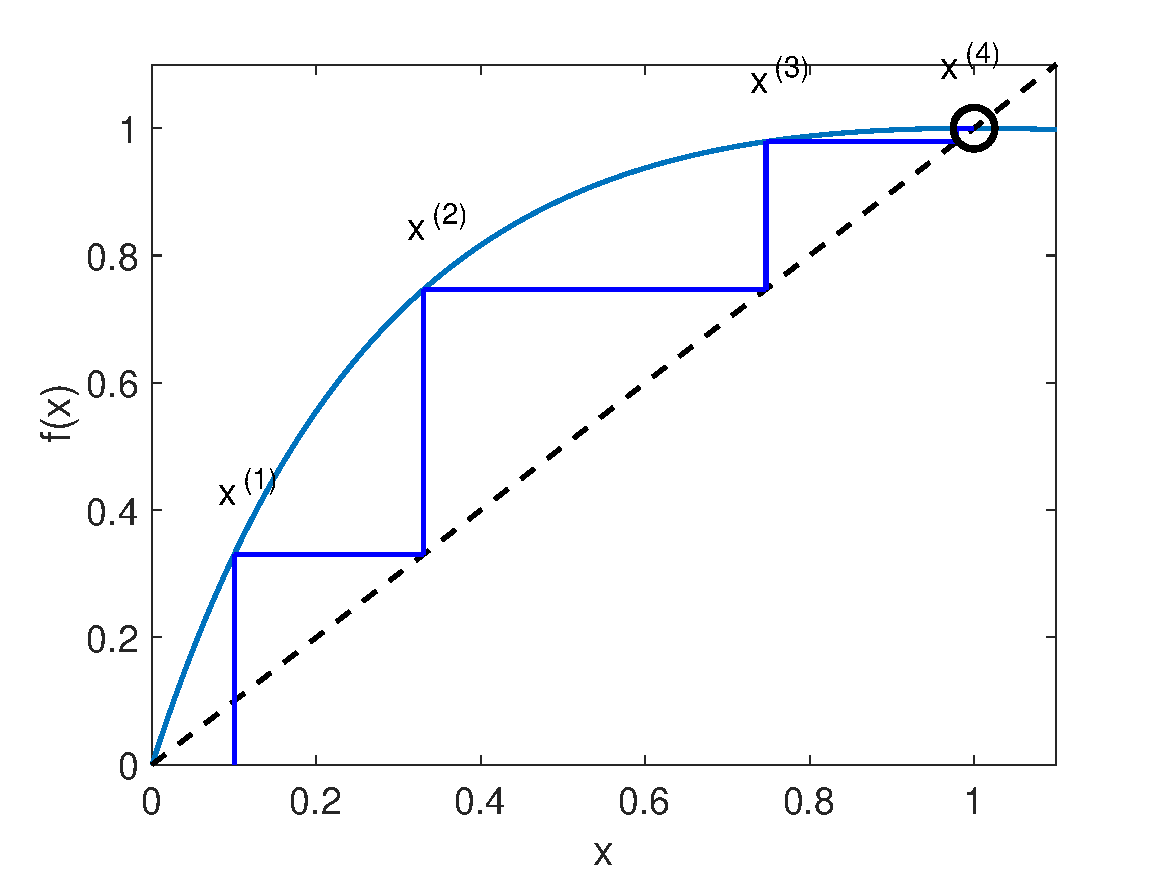
\includegraphics[width=7cm]{NRG_ising}
\caption{{\bf Recursion relation for $x$ in the 1d Ising model. Starting with an arbitrary $x^{(1)}\in(0,1]$ the fixed point is $x^{(\infty)}=1$. Only for
$x^{(1)}=0$ the other fixed point $x^{(\infty)}=0$ is relevant.}}
\label{fig:RNG_ising_x}
\end{center}
\end{figure}
The figure illustrates that if we start the recursion with any value $0< x^{(1)}\le 1$, i.e. $0\le  K< \infty$, which 
corresponds to the parameter of the original physical system, the iteration ends at the fixed point 
$x^{(\infty)}=1$. This means that the physical features (e.g. spin-spin correlation)
for very long distances is equivalent to that of an Ising model with $x=1$, which corresponds to $K=0$. This fixed point is called {\em high temperature fixed point}, as
$x=1$, or rather $K=0$ is also obtained for $T\to \infty$ ($\beta\to 0$).
The 1d Ising model considered at very long length scales looks like an infinite temperature 
or non-interacting solution, which means it is disordered (no long range order).
This fixed point is stable or attractive.

The other fixed point $x^{*}=0$ is the non-trivial {\em critical fixed point}.  It corresponds to $K=\infty$, i.e. $T=0$.
In this case, starting with the physical parameter $x=0$, i.e. $T=0$, the system stays at $x=0$
and is therefore ordered even over long range. This is the trivial case: At $T\to 0$ there are no thermal fluctuations, since there are no quantum fluctuations. Accordingly, the spins of such a 1-dimensional Ising will be ordered no matter how far the considered spins lie apart from each other. This result is in contrast to the case of the spin-$1/2$ Heisenberg model.

% Here it is the trivial case, without thermal fluctuations, there
% is long range order, since there are no quantum fluctuations,
% in contrast to the case of the spin-$1/2$ Heisenberg model.




\subsubsection{Energy Parameter}
Next we study the energy parameter $C$ for the case $h=0$. Then we have
%
\begin{align}\label{eq:RNG:Energy:parameter}
 C^{(n+1)} &= 2 C^{(n)} + \frac{1}{2}\ln\bigg(\cosh(2K^{(n)})\bigg)+ \ln(2) \;.
\end{align}
%
As the recursion for $K^{(n)}$ is independent of that for
$C^{(n)}$, we can insert the previous result for $K^{(n)}$. Hence for $n\to\infty$ (very long length scale),we have $K^{(n)}\to 0$ (or $x\to 1$ in \autoref{fig:RNG_ising_x}) and we find
%
\begin{align*}
 C^{(n+1)} &= 2C^{(n)} + \ln(2)\;.
\end{align*}
%
The factor $2$ is obvious due to the decimation of the number of spins by the factor $2$.

\subsubsection{Correlation length}
Next we want to discuss the correlation length, For that we first 
introduce a different  recursion relation for  $K^{(n)}$ (still for the case $h=0$).
From \eq{eq:rec:rel:K}  we obtain
%
\begin{align}\label{eq:rec:rel:K:b}
K^{(n+1)}  &= g(K^{n})\\
g(K) &= \frac{1}{2} \ln\bigg(\cosh(2 K) \bigg)\;,
\end{align}
which for large $K^{(n)}$ can be rewritten as follows
\begin{align*}
K^{(n+1)}  &= \frac{1}{2} \ln\bigg(\frac{e^{2 K^{(n)}}(1+e^{-4 K^{(n)}})}{2}\bigg)\\
&= K^{(n)} - \frac12 \ln(2) + \frac12\ln\big(1+e^{-4 K^{(n)}}  \big)\;.
\end{align*}
Hence we have for large $K^{(n)}$
\begin{align}\label{eq:rec:rel:K:c}
K^{(n+1)}&\approx K^{(n)} - \frac{\ln(2)}{2}\;.
\end{align}
%
If this relation applies, then
%
\begin{align}
K^{(n)}&\approx K^{(n-1)} - \frac{\ln(2)}{2}\nonumber\\
&\approx K^{(n-2)} - \frac{\ln(2)}{2} - \frac{\ln(2)}{2}\nonumber\\
&\cdots\nonumber\\
K^{(n)}&\approx K^{(0)} - \frac{n}{2}\cdot\ln(2)\;.
\label{eq:RG:iter}
\end{align}
%
Note that here we begin the iteration counter with index 0.
Now we want to use the renormalization group approach to study how the
correlation length depends on $\beta$ or rather $K$.
If there is no long range order, the spin-spin correlation  decreases exponentially as
\begin{align*}
\langle s_{0}s_{m} \rangle &\propto e^{-m/\xi(K)}\;.
\end{align*}
%
The correlation length $\xi(K)$ will depend on $\beta J = K$. In each renormalization step,
the unit cell increases by a factor of 2. 
In the original system we have
\begin{align*}
 \langle s_{0}s_{\red{2 m}} \rangle_{K^{(0)}} &\propto e^{-(\red{2 m})/\xi(K^{(0)})}\;.
\end{align*}
The same correlation function is equal to that of the renormalized system as follows
\begin{align*}
 \langle s_{0}s_{2 m} \rangle_{K^{(0)}} 
 = \langle s^{(2)}_{0}s^{(2)}_{m} \rangle_{K^{(1)}} 
 &\propto  e^{-m/\xi(K^{(1)})}\;.
\end{align*}
Comparing the exponentials yields
\begin{align*}
\xi(K^{(0)}) &= 2 \xi(K^{(1)})=2 \xi(g(K^{(0)}))\;.
\end{align*}
Repeating the renormalization $m$ times we obtain the relation
\begin{align}\label{eq:corr:length}
 \xi(K^{(0)}) &= 2^{m} \xi(g^{(m)}(K^{(0)})) \;.
\end{align}
The left hand site is the quantity we are interested in for low temperature or rather $K\gg 1$. In this case, according to \eq{eq:RG:iter}, after $m$ RNG steps we have
\begin{align*}
g^{(m)}(K^{(0)}) &= K^{(m)} \approx  K^{(0)} - \frac{m}{2} \ln(2)\;.
\end{align*}
Remember we are interested in $K\gg 1$. Each iteration reduces $K$ by $\ln(2)/2\approx 0.35$. Then
if we choose $m$ sufficiently large, eventually, we will reach an iteration $m^{*}$ with $K^{(m^{*})}=g^{(m^{*})}(K^{(0)})\sim O(1)$.
The required number of steps is
\begin{align*}
K^{(0)} - \frac{m^{*}}{2}\ln(2) &= \order{1}\\
m^{*} &= \frac{2 \big(K^{(0)}-\order{1}\big)}{\ln(2)} \\
m^{*} &\approx \frac{2 K^{(0)}}{\ln(2)}\;.
\end{align*}
Along with \eq{eq:corr:length} we obtain for $m=m^{*}$ RNG iterations (from now on we omit the upper index 0)
\begin{align*}
 \xi(K) &= 2^{m^{*}} \xi(\underbrace{
g^{(m^{*})}(K)
}_{\color{blue} = \order{1}}) \;.
\end{align*}
Now $g(K=\order{1})$ is some unimportant constant $C$ and we finally have
\begin{align*}
 \xi(K) &\sim  2^{m^{*}} = 2^{\frac{2 K}{\ln(2)}} 
=  e^{\ln(2^{\frac{2 K}{\ln(2)}})} 
=  e^{2 K}\;.
\end{align*}
\tboxit{Correlation length}{
\begin{align}\label{eq:corr:length:b}
 \xi(K) &\sim   e^{2 K}\;.
\end{align}}

\blue{So the bottom line is that the correlation length increases exponentially with decreasing 
temperature and becomes infinite at $T=0$, but it is finite for finite $T$ in agreement to the previous finding that there is no long range order for $T>0$.}

\subsubsection{Free Energy}
Finally, we compute the free energy for the case $h=0$. We start out from the partition function for the original system
and integrate out the spins on the odd sites and use \eq{eq:RNG:Z3} .
%
\begin{align*}
Z_{N}(K,C)&= \tr{e^{-\beta H}}
= \tr{e^{K\sum_{\langle ij \rangle}s_{i}s_{j}+N C}}=Z_{N/2}(K',C')\;,
\end{align*}
%
with $K'$ given in \eq{eq:rec:rel:K:b} and $C'$ given in 
\eq{eq:RNG:Energy:parameter}
%
\begin{align}\label{eq:renorm:C}
K^{(1)} &= \frac{1}{2}\ln\bigg(\cosh(2K^{(0)})\bigg)\\
C^{(1)}&= 2 C^{(0)} + K^{(1)} + \ln(2) \;.\label{eq:renorm:Cp}
\end{align}
%
Next, we express the partition function slightly differently by prepending $C$
%
\begin{align}\label{eq:Z:N:aux}
Z_{N}(K,C) = e^{N C^{(0)}} Z^{(0)}_{N}(K^{(0)}) = e^{\frac{N}{2} C^{(1)}} Z^{(0)}_{N/2}(K^{(1)})\;.
\end{align}
%
Taking the logarithm per lattice site (apart from a factor $(-k_{B}T)$ this is the free energy per lattice site)
%
\begin{align}
f(K^{(0)},C^{(0)})&=\frac{\ln\big(Z_{N}(K^{(0)},C^{(0)})\big)}{N} = C^{(0)} + \underbrace{
\frac{\ln\big(Z^{(0)}_{N}(K^{(0)})\big)}{N}
}_{\color{blue} := \tilde f(K^{(0)})}\notag\\
f(K^{(0)},C^{(0)})&= C^{(0)} + \tilde f(K^{(0)}) \;.\label{eq:f:K}
\end{align}
%
On the other hand, based on the second equation in \eq{eq:Z:N:aux} we obtain
%
\begin{align*}
f(K^{(0)},C^{(0)})
&= \frac{1}{N}\bigg( \frac{N}{2} C^{(1)} + \ln\big(Z^{(0)}_{N/2}(K^{(1)})  \big) \bigg)\\
%&=\frac{1}{2} C' + \frac{\ln\big(Z^{(0)}_{N/2}(K^{(1)})  \big)}{N}\\
&=\frac{1}{2} \qty( C^{(1)} + \frac{\ln\big(Z^{(0)}_{N/2}(K^{(1)})  \big)}{N/2} )\\
f(K^{(0)},C^{(0)})&=\frac{1}{2}\bigg( C^{(1)} + \tilde f(K^{(1)}) \bigg)\;.
\end{align*}
%
Comparison  with \eq{eq:f:K} gives
%
\begin{align*}
 \tilde f(K^{(0)}) &=\frac{1}{2}\bigg( C^{(1)}-2 C^{(0)} + \tilde f(K^{(1)}) \bigg)\;.
\end{align*}
%
Inserting \eq{eq:renorm:Cp} finally yields
\begin{align}\label{eq:one:iteration} 
 \tilde f(K^{(0)}) &=\frac{1}{2}\bigg( K^{(1)} + \ln(2)+ \tilde f(K^{(1)})  \bigg)\;
\end{align}
%
From a second iteration we get
\begin{align*}
\tilde f(K^{(1)}) &= \frac{1}{2}\bigg(K^{(2)} + \ln(2)+ \tilde f(K^{(2)}) \bigg)\;.
\end{align*}
%
Inserting into \eq{eq:one:iteration}  yields
%
\begin{align*}
\tilde f(K^{(0)}) &= 
\frac{1}{2}
\bigg(
K^{(1)}+\ln(2) +
\frac{1}{2}
\bigg[  
K^{(2)}+\ln(2) + \tilde f(K^{2)}
\bigg]
  \bigg)\\
  &= \frac{K^{(1)}+ln(2)}{2^{1}} +\frac{K^{(2)}+ln(2)}{2^{2}} + \frac{\tilde f(K^{(2)}) }{2^{2}}\;.
\end{align*}
%
Clearly, this leads after $m$ iterations to
\begin{align*}
\tilde f(K^{(0)}) &=\sum_{\nu=1}^{m} \frac{\ln(2)}{2^{\nu}} +\sum_{\nu=1}^{m} \frac{K^{(\nu)}}{2^{\nu}} + \frac{\tilde f(K^{(m)}) }{2^{m}}\\
&=\ln(2)\sum_{\nu=1}^{m} \frac{1}{2^{\nu}}  +\sum_{\nu=1}^{m} \frac{K^{(\nu)}}{2^{\nu}} + \frac{\tilde f(K^{(m)}) }{2^{m}}\\
&=\ln(2)\sum_{\nu=1}^{m} \frac{1}{2^{\nu}}  +\sum_{\nu=1}^{m} \frac{K^{(\nu)}}{2^{\nu}} + \frac{\tilde f(K^{(m)}) }{2^{m}}\;.
\end{align*}
%
We have seen, that $K^{(n)}\to 0$ for $n\to\infty$. The partition function for $K\to 0$ can be
obtained analytically as
%
\begin{align*}
Z_{N}(K\to 0) &= 2^{N}\;,
\end{align*}
%
hence, according to the definition $\tilde f = \ln(Z)/N$, we obtain
%
\begin{align*}
\tilde f(K\to 0) &= \frac{\ln(Z_{N})(K\to 0) }{N} = \ln(2)
\end{align*}
%
So, if we perform an infinite number of  renormalization steps, we obtain
%
\begin{align*}
\tilde f(K^{(0)}) &= \ln(2)
\underbrace{
\bigg( \sum_{\nu=0}^{\infty} \big(\frac{1}{2}\big)^{\nu} -1\bigg)
}_{\color{blue} = 1}
+\sum_{\nu=1}^{\infty} \frac{K^{(\nu)}}{2^{\nu}} + \underbrace{
\lim_{L\to\infty}\frac{\ln(2)}{2^{L}}
}_{\color{blue} = 0}\\
&= \ln(2)+\sum_{\nu=1}^{\infty} \frac{K^{(\nu)}}{2^{\nu}}\;.
\end{align*}
%
We have seen in chapter 1 that the exact result is given by
%
\begin{align*}
Z_{N} &=  d_{1}^{N}\\
\tilde f(K) &= \ln(d_{1})\\
d_{1} &= 2 \cosh(K^{0})\;,
\end{align*}
%
Hence, since $C^{(0)}=0$
%
\begin{align*}
f(K^{(0)},C^{(0)}) &= \tilde f(K^{(0)}) = \ln(2) + \ln(\cosh(K^{(0)}))\;.
\end{align*}
%
Numerical comparison shows that both results agree, i.e.
%
\begin{align*}
\sum_{\nu=1}^{\infty} \frac{K^{(\nu)}}{2^{\nu}} &= 
\ln(\cosh(K^{(0)}))\intertext{with}
K^{(n)} &=\frac{1}{2}\ln\bigg( \cosh (2 K^{(n-1)}) \bigg)\;.
\end{align*}
%


In the 1D case, no approximations were necessary for the RNG procedure.






\section{2D Ising}

We decompose the sc-lattice into an A-B-lattice, i.e. sites belong  either to 
sub-lattice A (blue circles with even indices) or B (red crossed with odd indices). 
All nearest neighbors of a point of sub-lattice A belong to sub-lattice B and vice versa. 

%
\begin{figure}[htbp]
\begin{center}
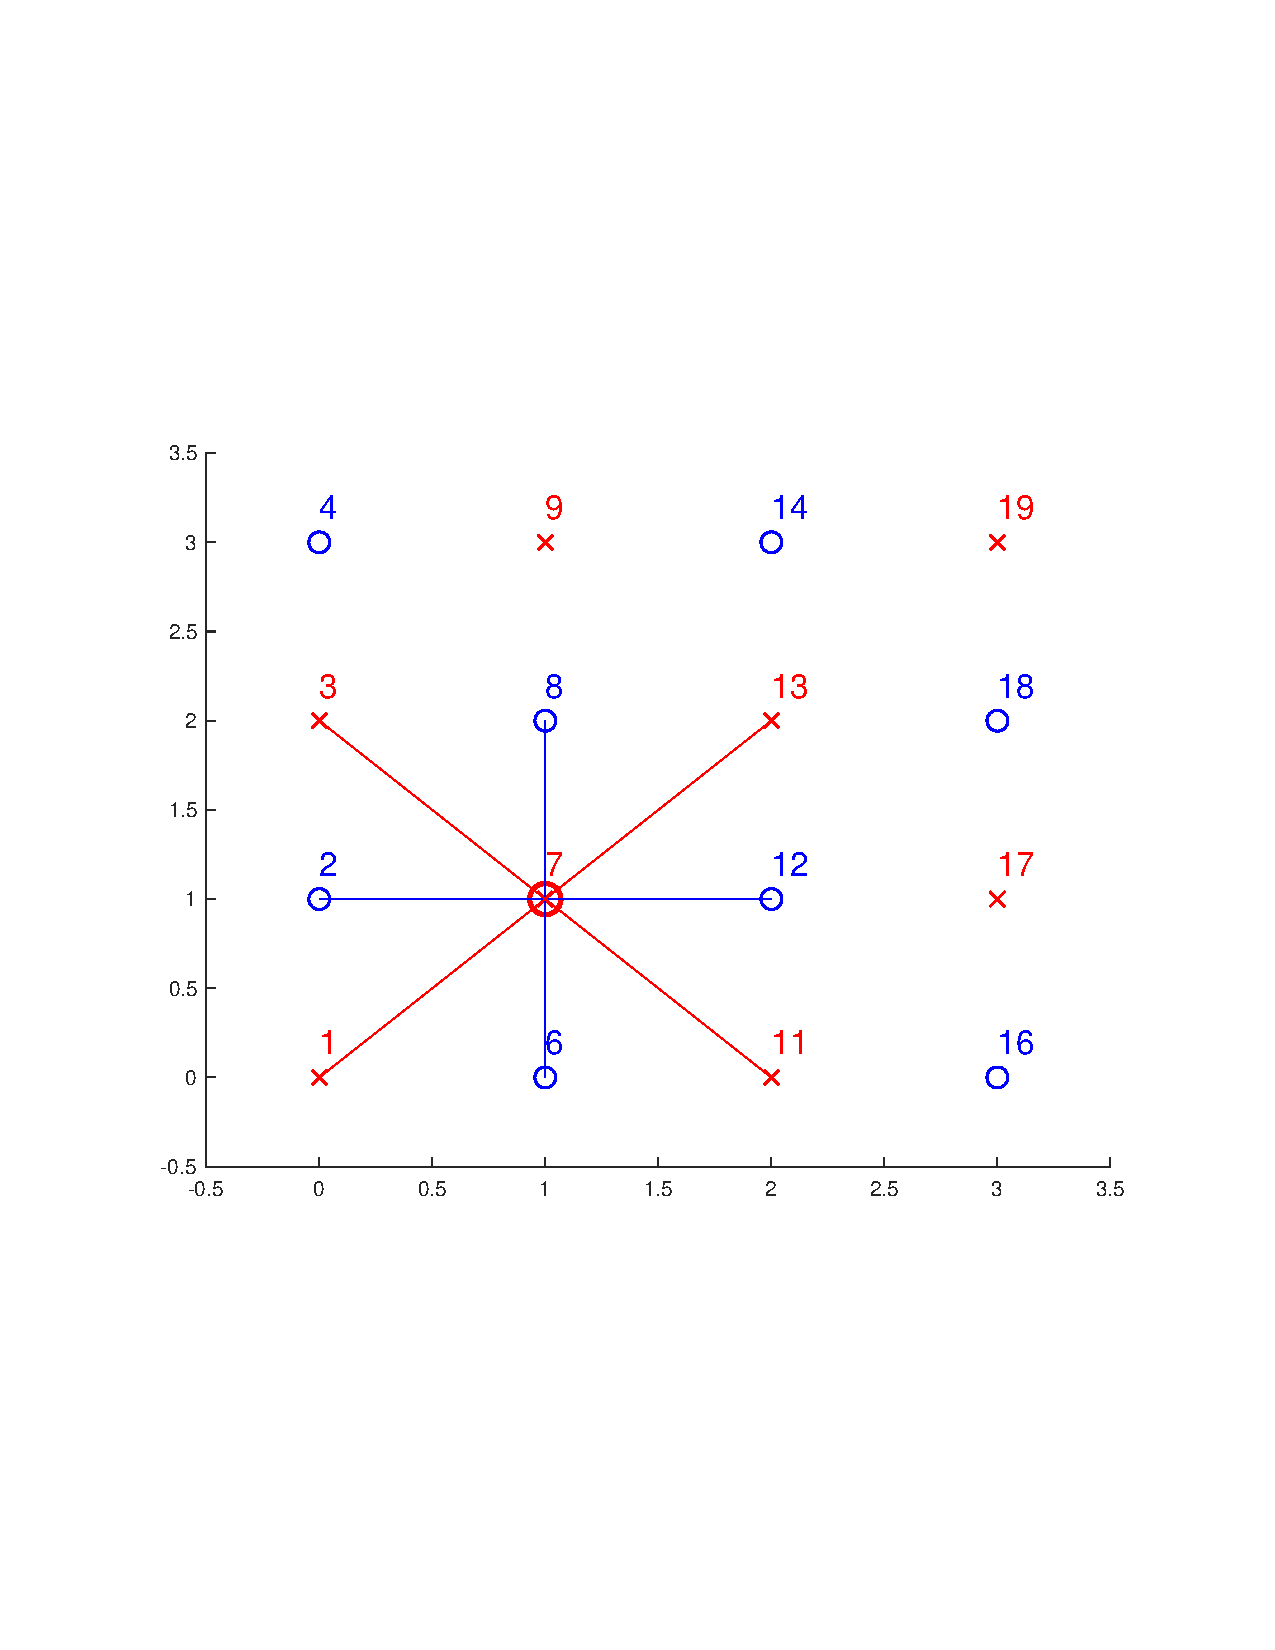
\includegraphics[width=7cm]{RRG_Ising_2D}
\caption{\bf Illustration of the RG scheme for 2D Ising. 
}
\label{fig:rng:ising:2d} 
\end{center}
\end{figure}
%
The goal is again to decimate the lattice by integrating out sublattice B, i.e.
to compute the reduced density matrix for sub-lattice A.
The reduced density matrix on sub-lattice A is
%
\begin{align*}
\rho_{A} &= \sum_{\{S_{i}\}\in B} e^{-\beta H}
\end{align*}
%
To get an idea of one renormalization step,
we consider all terms of the hamiltonian that contain the spin on site 7, which is part of sub-lattice B.
%
\newcommand{\Snn}{{\cal S}^\text{nn}_{7}}
\newcommand{\Snnn}{{\cal S}^\text{nnn}_{7}}
\begin{align*}
-\beta H_{7} &= C + h S_{7} + K \Snn S_{7 }\\
\Snn &= S_{2} + S_{6} + S_{8} + S_{12}\;.
\end{align*}
%
Next we separate the contribution of this spin from the rest
%
\begin{align*}
\rho_{A} &= \sum_{\{S_{i}\}\in B / S_{7}} e^{-\beta H'} \cdot Z_{7}\\
Z_{7} &= \sum_{S_{7}} e^{-\beta H_{7}}
\end{align*}
% 
with $H'=H-H_{7}$ being the hamiltonian without site 7.
The trace over $S_{7}$ yields
%
\begin{align}\label{eq:Z:7a}
Z_{7}:=
\sum_{S_{0}} e^{C + S_{7}\big( K \;\Snn +h\big) }
&= e^{C} \cdot 2\cosh\big(K \Snn  +h  \big)\;.
\end{align}
%
We want to express this function again as
%
\begin{align*}
e^{- \beta \tilde H}\;.
\end{align*}
%
The most general exponential form for this expression, since $S_{i}^{2}=1$, is given by
%
\begin{align}\label{eq:Z7}
Z_{7}&= \exp\bigg(C' + h' {\cal S}_{7}	^{nn}\;.
+ \overline{K} \sum'_{ij}  S_{i}S_{j}  +
b \sum'_{ijk} S_{i}S_{j} S_{k}  + c \; S_{2}S_{6}S_{8}S_{12}\bigg)\;.
\end{align}
%
The indices in the sums are from the set $I^{nn}_{7} =\{2,6,8,12\}$,
and the prims indicate that  no indices must occur twice and all the indices shall be ordered, e.g. $S_{i}<S_{j}<S_{k}$. 
We have used the symmetry that \eq{eq:Z:7a}
is invariant against interchange of any two indices $i\leftrightarrow j$.
Otherwise , each product of spins would have its own prefactor.

In the double sum there are also the products  $S_{6} S_{8}$ and $S_{2} S_{12}$,
which belong to next-nearest neighbour sites on the decimated lattice, which only consists of sub-lattice A (blue circles). I.e. starting from nn coupling
the decimation also introduces nnn coupling and also terms with three and four spins.
The latter will turn out negligible but the nnn coupling is relevant. 
To obtain the parameter mapping in an RG step, we include the nnn terms also in the original hamiltonian, i.e. 
\begin{align*}
-\beta H_{7} &= C + S_{7} \qty(h  + K  \Snn +L \Snnn)\\
\Snn &= S_{2} + S_{6} + S_{8} + S_{12}\\
\Snnn &= S_{1} + S_{3} + S_{11} + S_{13}\;.
\end{align*}
%
Again, we separate the contribution of this spin from the rest


%
\begin{align*}
\rho_{A} &= \sum_{\{S_{i}\}\in B / S_{7}} e^{-\beta H'}\cdot Z_{7}\\
Z_{7} &= \sum_{S_{7}} e^{-\beta H_{7}}
\end{align*}
% 
The trace over $S_{7}$ now yields
%
\begin{align}\label{eq:Z:7}
Z_{7}&= e^{C} \cdot 2\cosh\big(K \Snn  + L \Snnn + h  \big)\;.
\end{align}
%
Here we have a problem, since $\Snnn$ contains spins of sublattice B (e.g. $S_{13}$)
that still need to be integrated out and that are also contained in the   
residual hamiltonian  $H'$. In this combination the sum over $S_{13}$ is not as trivial as
that over $S_{7}$, which we had before. Moreover, the complexity increases, as $Z_{7}$
also contains other spins of sub-lattice $B$ ($S_{1}$ say) and after the trace over $S_{13}$ the expression containing $S_{1}$ is getting even more complicated, etc..
Hence, to keep things manageable, we replace  $\Snnn$ at this point by its mean value, which is zero.
Then we are left with
%
\begin{align}\label{eq:Z:7b}
Z_{7}&= e^{C} \cdot 2\cosh\big(K \Snn  + h  \big)\;.
\end{align}
%
\blue{As we will see soon, that does not mean that the original nnn coupling has no influence at all.}
We can use the general exponential from of \eq{eq:Z7} again
%
\begin{align*}
Z_{7} &= \exp\bigg(C' + h' {\cal S}+ \overline K \sum'_{ij}  S_{i}S_{j}  +
b \sum'_{ijk} S_{i}S_{j} S_{k}  + c \; S_{2}S_{6}S_{8}S_{12}\bigg)\;.
\end{align*}
%
As before, the indices in the sums are from the set $I^{nn}_{7} =\{2,6,8,12\}$.
The term with 3 spins can equivalently be written as
%
\begin{align*}
\sum'_{ij} S_{i}S_{j}S_{k}   &= {\cal S} \cdot  S_{2}S_{6}S_{8}S_{12} 
\end{align*}
%
\emphasize{proof}{
%
\begin{align*}
\sum'_{ij} S_{i}S_{j}S_{k}  
&= S_{2}S_{6}S_{8}
+ S_{2}S_{6}S_{12}
 + S_{2}S_{8}S_{12}
  + S_{6}S_{8}S_{12}\\
  &= S_{2}S_{6}S_{8} S_{12}^{2}
+ S_{2}S_{6}S_{12} S_{8}^{2}
 + S_{2}S_{8}S_{12} S_{6}^{2}
  + S_{6}S_{8}S_{12} S_{2}^{2}\\
  &=S_{2} S_{6}S_{8}S_{12} \big( S_{12}+S_{8}+S_{6} +S_{2x^{}}\big)
\end{align*}
}

So we have the constraint
%
\begin{align}\label{eq:constr}
C + \ln\bigg(2\cosh\big[K{\cal S} +h  \big]  \bigg)&=
C' + h' {\cal S} + \overline K \sum'_{ij} S_{i}S_{j}  +
\bigg(b{\cal S} + c\bigg) S_{1}S_{2}S_{3}S_{4}
\end{align}
%
Now we consider this constraint for all possible spin configurations:
%
\begin{align*}
1)&&(++++)&:&C + \ln\bigg(2\cosh\big[4 K+h  \big]  \bigg) &=
C' + 4 h'  + 6 \overline K   + \big(4b+c\big)\cdot 1 \\
2)&&(+++-)&:&C + \ln\bigg(2\cosh\big[2 K+h  \big]  \bigg) &=
C' + 2 h'  + 0 \overline K   + \big(2b+c\big)\cdot (-1) \\
3)&&(++--)&:&C + \ln\bigg(2\cosh\big[0K+h  \big]  \bigg) &=
C' + 0 h'  - 2 \overline K   + \big(0b+c\big)\cdot 1 \;
\end{align*}
%
Since the geometric position of the spins does not enter in \eq{eq:constr} we get the same equations if we permute the spins.

%
The remaining spin configurations
are obtained by the transformation $S_{i}\to - S_{i}$, which changes the sign in the terms with an odd number of spins. I.e. 3) is invariant, and for the other two we obtain
\begin{align*}
1')&&(----)&:&C + \ln\bigg(2\cosh\big[-4 K+h  \big]  \bigg) &=
C' - 4 h'  + 6 \overline K   + \big(-4b+c\big)\cdot 1 \\
2')&&(---+)&:&C + \ln\bigg(2\cosh\big[-2 K+h  \big]  \bigg) &=
C' - 2 h'  + 0 \overline K   + \big(-2b+c\big)\cdot (-1) \\
\end{align*}
%
We simplify these equations a bit further
\begin{align*}
1)&&(++++)&:& \ln\bigg(2\cosh\big[4 K+h  \big]  \bigg) &=
\Delta C + 4 h'  + 6 \overline K   + 4b+c \\
1')&&(----)&:& \ln\bigg(2\cosh\big[-4 K+h  \big]  \bigg) &=
\Delta C  - 4 h'  + 6 \overline K   -4b+c \\
2)&&(+++-)&:&\ln\bigg(2\cosh\big[2 K+h  \big]  \bigg) &=
\Delta C + 2 h'   - 2b-c \\
2')&&(---+)&:&\ln\bigg(2\cosh\big[-2 K+h  \big]  \bigg) &=
\Delta C - 2 h'     + 2b-c\\
3)&&(++--)&:& \ln\bigg(2\cosh\big[h  \big]  \bigg) &=
\Delta C - 2 \overline K   + c \;,
\end{align*}
%
with $\Delta C = C'-C$. 

%
When we add or subtract equation 1 and 1' and likewise for 2 and 2', we obtain
%
\begin{align*}
a)&:& \ln\bigg(4\cosh\big[4 K+h  \big] \cosh\big[4 K-h  \big] \bigg) &= 2\bigg( 
  \Delta C + 6\overline K +c   \bigg)\\
a')&:&  \ln\bigg(\cosh\big[4 K+h  \big]/ \cosh\big[4 K-h  \big] \bigg) &= 8\big( h' +b
 \big)\\
b)&:&2\ln\bigg(4\cosh\big[2 K+h  \big]\cosh\big[2 K-h  \big]  \bigg) &=
4\bigg( \Delta C -c \bigg)\\
b')&:&2\ln\bigg(\cosh\big[2 K+h  \big]/\cosh\big[2 K-h  \big]  \bigg) &=
8\bigg(h' -b \bigg)\;.
\end{align*}
Equation 3) yields
%
\begin{align*}
c)\Delta C +c   &=
\ln\bigg(2\cosh\big[h  \big]  \bigg) + 2 \overline K
\end{align*}
%
  
%
Inserting c) into a) gives
\begin{align*}
\tilde a)&:& \ln\bigg(4\cosh\big[4 K+h  \big] \cosh\big[4 K-h  \big] \bigg) &= 2
 \ln\bigg(2\cosh\big[h  \big]  \bigg)+ 16\overline K   \\
&&16 \overline K &= \ln\bigg(
\frac{\cosh\big[4 K+h  \big] \cosh\big[4 K-h  \big] }{\cos^{2}([h]}
  \bigg)
\end{align*}
%
We see that $\overline K$ only depends on $K$ and $h$.
If we add a') and b') we obtain
%
\begin{align*}
16 h' &=
\ln\bigg( 
\frac{\cosh\big[4 K+h  \big]\cosh^{2}\big[2 K+h  \big]}{\cosh\big[4 K-h  \big]\cosh^{2}\big[2 K-h  \big]  }
 \bigg)\;.
\end{align*}
%
Also $h'$ only depends on $h$ and $K$. Especially for $h=0$, we find $h'=0$. So 
the renormalization does not introduce a B-field, when we start with $B=0$. 

%%
%\begin{align*}
%e^{-16 \overline K} &= 
%\frac{\cosh^{2}(h)}{\cosh\big[4 K+h  \big] \cosh\big[4 K-h  \big] }
%=
%\frac{(e^{h}+e^{-h})^{2}}{(e^{4 K+h }+e^{-4 K-h}) (e^{4 K-h }+e^{-4 K+h}) }\\
%&=
%\frac{e^{2h} (1+e^{-2h})^{2}}{e^{8K}e^{2h}(1+e^{-8 K-2h}) (e^{-2h }+e^{-8 K}) }\\
%&=e^{-8K}
%\frac{(1+e^{-2h})^{2}}{(1+e^{-8 K-2h}) (e^{-2h }+e^{-8 K}) }\\
%e^{-16 h'} &=
%\frac{\cosh\big[4 K-h  \big]\cosh^{2}\big[2 K-h  \big]  }{\cosh\big[4 K+h  \big]\cosh^{2}\big[2 K+h  \big]}\\
%&=
%\frac{(e	^{4 K-h}+e	^{-4 K+h})  (e^{2 K-h}+e^{-2 K+h})^{2}   }
%{(e	^{4 K+h}+e	^{-4 K-h}) (e^{2 K-h}+e^{-2 K+h})^{2}   }\\
%&=
%\frac{e^{8K}(e	^{-h}+e	^{-8K+h})  (e^{-h}+e^{-4 K+h})^{2}   }
%{e^{8K}(e	^{h}+e	^{-8 K-h}) (e^{-h}+e^{-4 K+h})^{2}   }\\
%&=
%\frac{e^{3h}(e	^{-2h}+e	^{-8K})  (e^{-2h}+e^{-4 K})^{2}   }
%{e^{3h}(1+e	^{-8 K-2h}) (e^{-2h}+e^{-4 K})^{2}   }\\
%&=
%\frac{(e	^{-2h}+e	^{-8K})  (e^{-2h}+e^{-4 K})^{2}   }
%{(1+e	^{-8 K-2h}) (e^{-2h}+e^{-4 K})^{2}   };.
%\end{align*}
%
%%
%\begin{align*}
%e^{-16 \overline K} 
%&=e^{-8K}
%\frac{(1+e^{-2h})^{2}}{(1+e^{-8 K-2h}) (e^{-2h }+e^{-8 K}) }\\
%e^{-16 h'}
%&=
%\frac{(e	^{-2h}+e	^{-8K})  (e^{-2h}+e^{-4 K})^{2}   }
%{(1+e	^{-8 K-2h}) (e^{-2h}+e^{-4 K})^{2}   };.
%\end{align*}
In the following we will consider only the case $h=0$. Then we obtain  

%
\begin{align}\label{eq:ol:K}
\overline K &= \frac{1}{16}\ln(\cosh^{2}[4 K])
= \frac{1}{8}\ln(\cosh[4 K])\;.
\end{align}
%
Later on we will also need the derivative
%
\begin{align}\label{eq:der:ul:K}
\alpha(K) &= \dv{\overline K(K)}{K} =\frac{1}{2} \tanh(4 K)
\end{align}
%
For the determination for the other parameters for $h=0$ we have to solve

%
\begin{align*}
b)&\Rightarrow \overline{b}& \ln\bigg(2\cosh\big[2 K\big] \bigg) &=
\Delta a -c \tag{$\overline b$}\\
b')&\Rightarrow&0&= 8\big(h' -b \big)\tag{$\overline b'$}\\
c)&\Rightarrow\overline{c}& \ln(2) + 2 \overline K &=\Delta a +c   \tag{$\overline c$}
\end{align*}
%


We know already that $h=0$ also means $h'=0$ and according to $\overline b'$ this implies    $b=0$. 
I.e. the three-spin coupling  vanishes, which is reasonable, because without an external B-field no spin-direction  is favoured, i.e. the hamiltonian is invariant under the reversion of all spins. This symmetry would be violated by the three-spin coupling.
Finally, $\overline c$ - $\overline b$ yields
%
\begin{align}\label{eq:four:spin:term}
c &= \overline K  - \frac{1}{2}\ln(\cosh(2 K))
\end{align}
%



In addition, from $\overline c + \overline b$ we obtain
%
\begin{align*}
\Delta a &= \frac{1}{2}\qty( 2\ln(2) +  \ln(\cosh(2K)) +    2 \overline K )\;.
\end{align*}
%
Along with \eq{eq:ol:K} we obtain
%
\begin{align}\label{eq:Delta:a}
\Delta a &=   \ln(2) + \frac{1}{2}\ln(\cosh(2K))  + \frac{1}{8}\ln(\cosh(4 K)) \\
\Delta a &=   \ln(2 \cosh^{\frac{1}{2}}(2K)\cosh^{\frac{1}{8}}[4 K]) \;.
\end{align}
%


\subsubsection{First approximation, ignoring nnn interaction}
 
 
In \eq {eq:constr} we have the new two-spins interaction term in the decimated lattice, which is given by
%
\begin{align}\label{eq:E7}
E_{7}(S) :=
 \overline K \sum'_{ij} S_{i}S_{j} &=
 \overline K
\underbrace{
\qty(S_{2}S_{6}+S_{6}S_{12}+S_{12}S_{8}+S_{8}S_{2})
}_{\color{blue} = \text{nn terms in dec. lattice}}
+ \ldots\\
&+
\overline K
\underbrace{\qty(S_{2}S_{12}+S_{6}S_{8})}_{\color{blue} = \text{nnn terms in dec. lattice}}
\end{align}
%
This is the interaction that comes from the sum over $S_{7}$. 
Among others, there  is  a coupling between $S_{8}$ and $S_{12}$.
Integrating out $S_{13}$ also mediates a coupling between these spins. 
These contributions add up. Therefore, we 
have for the new nn coupling between site $8$ and $12$
%
\begin{align*}
K' &= 2 \overline K\;.
\end{align*}
%
Moreover, in addition to the nn coupling we also have a nnn
coupling in the decimated lattice. Both couplings 
support the same  (ferromagnetic) orientation. 
As a first approximation, we want to omit these terms and use 
a modified nn coupling instead.

We consider the isolated cluster with sites $2,6,8,12$ with $S_{7}$ being integrated out. For a perfect ferromagnetic alignment (all spins in the cluster equal +1)
we have for the energy of that cluster if we include the nnn term
%
\begin{align*}
E_{7}(S) &= 6 \overline K \;.
\end{align*}
%
Omitting the nnn term and using $\tilde K$ for the nn coupling instead, we find

%
\begin{align*}
\tilde E_{7}(S) &= 4 \tilde K \;.
\end{align*}
%
These energies shall be the same and we therefore use
%
\begin{align*}
\tilde K &= \frac{3}{2} \overline K\;. 
\end{align*}
%
As mentioned before, this coupling gets a factor two
by the integration of the neighbouring spins in the B sub-lattice.
Hence in this approximation we have
%
\begin{align}\label{eq:RG:2D:first}
K' &= 3 \overline K  = \frac{3}{8} \; \ln\bigg(  \cosh(4K)\bigg)\;.
\end{align}
%


%
\begin{figure}[htbp]
\begin{center}
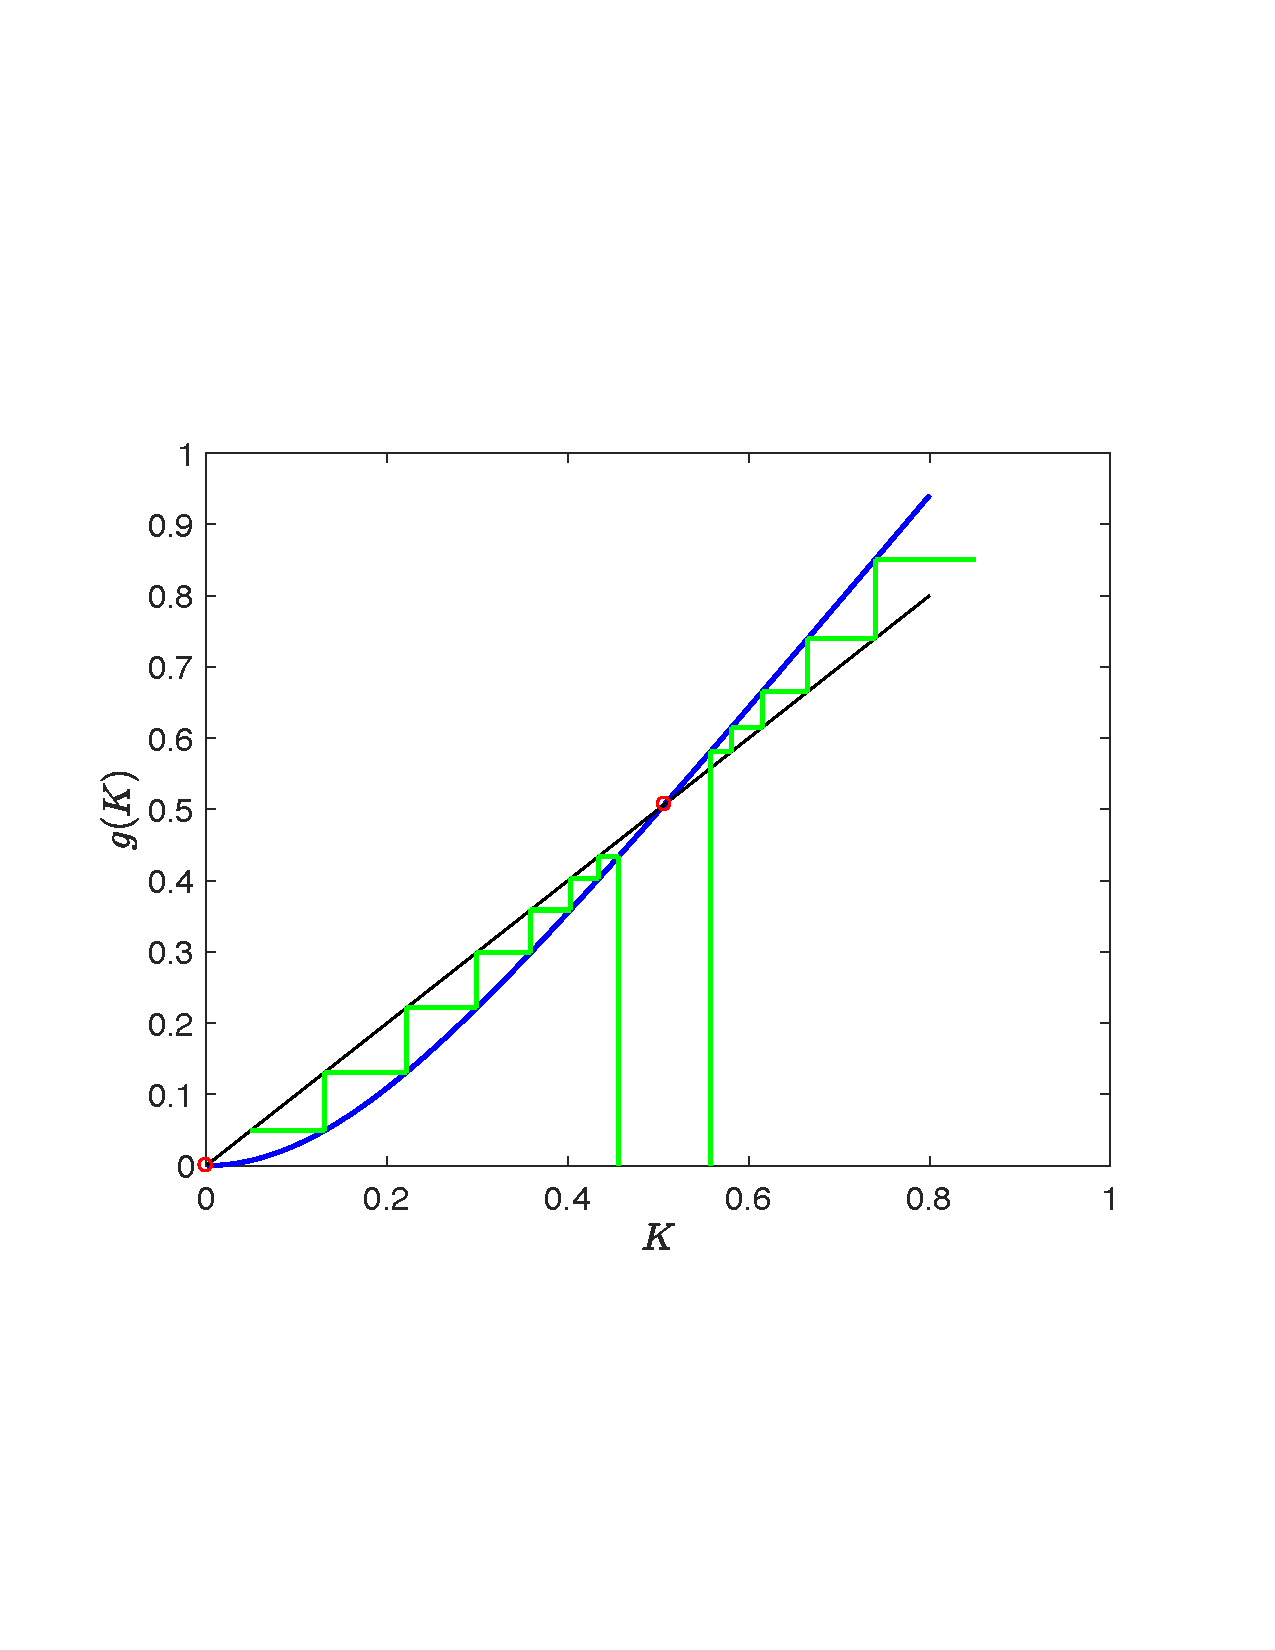
\includegraphics[width=7cm]{RNG_flow_2D}
\caption{\bf Flux of the renormalization iterations in the first approximation
described by equation (\ref{eq:RG:2D:first}).
}
\label{fig:rng:ising:2d}
\end{center}
\end{figure}



In \fig{fig:rng:ising:2d} the mapping of the coupling parameter $K$ during the renormalization
steps is depicted.
We find three fixed points, $K^*_{1}=0$, $K_{2}^{*}=\infty$, and $K^{*}_{3}=0.507$. 
The first two are the same as in the 1D case, \red{but with the important difference that now both fixed points are stable, while in the 1D case the
low-temperature fixed point $K^{*}=\infty$ was unstable.}
The $K^{*}=0$ fixed point is trivial and corresponds to $T=\infty$ where the correlations between neighboring spins vanish. The other fixed point ($K^{*}=\infty$) is a so-called critical fixed point as it describes the situation that the correlation length diverges for $T\to 0$
but there are nonetheless no fluctuations since all spins are perfectly aligned.
Only the third  fixed point describes a true \blue{critical point}. This one is   unstable. If we start with a physical parameter $K>K^{*}_{3}$ the interaction leads to $K=\infty$, while if we start with $K<K_{3}^{*}$ the iterations lead to $K=0$. Only starting precisely with $K=K^{*}_{3}$, the value of $K$ does not change.
So $K_{3}^{*} = \frac{J}{k_{B}T^{*}}$ corresponds to the phase transition. For $T<T^{*}$ 
($K>K^{*}_{3}$) the fixed point is $K\to \infty$, i.e. $T=0$ and hence long range order 
and in the other case the system behaves like $T=\infty$. 

The value $K^{*}_{3}=0.507$ has to be compared with the exact result
%
\begin{align*}
\beta^{*} J &= 0.4407\;.
\end{align*}
%
We have ignored so far the four-spin term. It has the coupling parameter $c$, which is given in 
\eq{eq:four:spin:term}. According to \eq{eq:RG:2D:first} we have
%
\begin{align*}
\overline K &= \frac{K'}{3}
\end{align*}

As the recursion equation for $K$ is independent of the other parameters, 
we can replace $K$ by its  fixed point values $K^{*}$ and we obtain
\begin{align}\label{eq:four:spin:term}
c &=  \frac{K^{*}}{3}  - \frac{1}{2}\ln(\cosh(2 K^{*})) = -0.053.
\end{align}
%
%
The result confirms that the four-spin coupling is much smaller than the two-spin terms
and can, therefore, be either ignored or taken into account perturbationally.





\subsubsection{Second approximation, including nnn interaction}


%
\begin{figure}[htbp]
\begin{center}
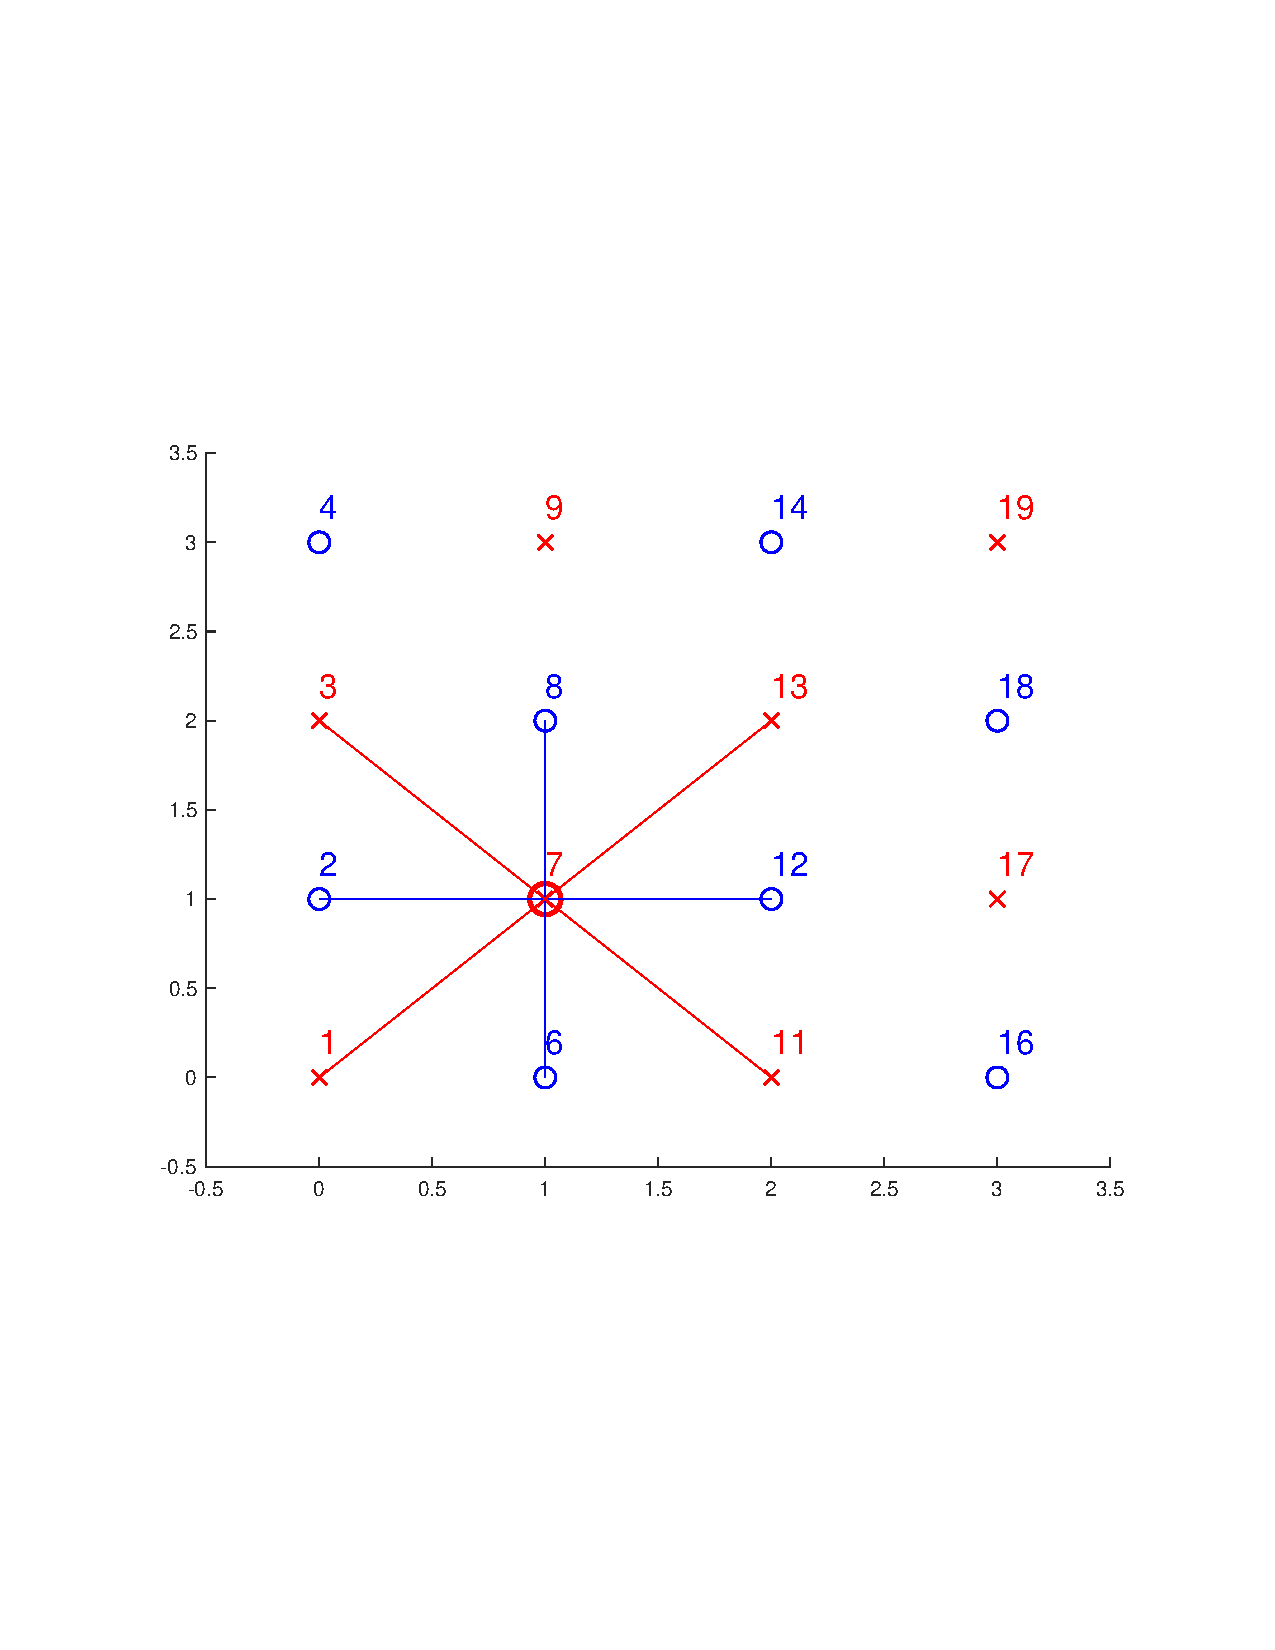
\includegraphics[width=7cm]{RRG_Ising_2D}
\caption{\bf Illustration of the RG scheme for 2D Ising. 
}
\label{fig:rng:ising:2d:b
} 
\end{center}
\end{figure}

As argued before the summation of $S_{7}$ and $S_{13}$ yield a nn 
coupling $2 \overline K$ for the nn spins $S_{8}$ and $S_{12}$, in the decimated lattice. In addition for the same spins, we still have the  nnn coupling $L$ of the original 
lattice, which is not modified by the summation over spins of the B sub-lattice.
Hence 
%
\begin{align}
K' &= 2 \overline K + L\;.
\end{align}
%
The  new nnn coupling in the decimated lattice (between $S_{2}$ and $S_{12}$, say),
is given by $\overline K$ 
\blue{(see second term on rhs of \eq{eq:E7}). The coupling of these spins  is only generated by summing over $S_{7}$; hence no factor 2)}. The total RG iteration for the parameters $K$ and $L$ is
%
\begin{align}\label{eq:RG:Ising:2D:b}
K' &= \frac{2}{8}\ln(\cosh[4K])    + L\\
L' &= \frac{1}{8}\ln(\cosh[4K])\;.
\end{align}
%
These equations have the following fixed points
\begin{align}\label{eq:RG:Ising:2D}
K^{*} &= \frac{2}{8}\ln(\cosh[4K^{*}])    + L^{*}\\
L^{*} &= \frac{1}{8}\ln(\cosh[4K^{*}])\;.
\end{align}
%
Inserting the second equation into the first gives
%
\begin{align*}
K^{*} &= \frac{3}{8}\ln(\cosh[4K^{*}])\;.
\end{align*}
%
This is the same fixed point equation as before in \eq{eq:RG:2D:first} , resulting in
$K_{1}^{*}=0, K_{2}^{*}=\infty$, and $K_{3}^{*}=0.507$.
For the unstable fixed point we have
%
\begin{align}
K^{*}_{3} &= 0.507\\
L^{*}_{3} &= \frac{K^{*}}{3} = 0.169\;.
\end{align}
%
Next we will analyse this fixed point in more detail and we will omit
the index for simplicity.
We consider the close neighbourhood of this fixed point and expand the iteration equation
%
\begin{align*}
K' &= 2 \overline K(K) + L\\
L' &= \overline K(K) \;,
\end{align*}
%
about the fixed point
%
\begin{align*}
K' &= 
\underbrace{2 \overline K(K^{*}) + L^{*}}_{\color{blue} = K^{*}} 
+ 2 \underbrace{
\eval{\frac{d \overline K(K)}{d K}}_{K^{*}}
}_{\color{blue} = \alpha^{*}}
\var  K
+ \var  L
\\
L' &= \underbrace{\overline K(K^{*})}_{\color{blue} = L^{*}} 
+ \underbrace{
\eval{\frac{d \overline K(K)}{d K}}_{K^{*}}
}_{\color{blue} = \alpha^{*}} \var  K
\end{align*}
%
The derivative is according to \eq{eq:der:ul:K}
%
\begin{align*}
\alpha^{*} &=  \frac{1}{2} \tanh(4 K^{*})
= 0.48297\;.
\end{align*}
%
Then with the definition  $\var \vv x = (\var K,\var L)^{T} = (K-K^{*},L-L^{*})^{T}$
we have
%
\begin{align*}
\var x'
&= 
\underbrace{
\mqty(2 \alpha^{*} & 1\\
\alpha^{*}&0
)
}_{\color{blue} = M}
\var x
\end{align*}
%
The matrix $M$ has the eigenvalues
%
\begin{align*}
\lambda_{\pm} &= \alpha^{*} \pm \sqrt{{\alpha^{*}}^{2} +\alpha^{*}}\\
\lambda_{+} &= 1.329282636504768\\
\lambda_{-} &= -0.363334404967798\;.
\end{align*}
%
and eigenvectors
%
\begin{align*}
\vv v_{\pm} &= 
\mqty(
\alpha^{*} \pm  \sqrt{{\alpha^{*}}^{2}+\alpha^{*}}\\\alpha^{*}
)\;.
\end{align*}
%

%
\begin{figure}[htbp]
\begin{center}
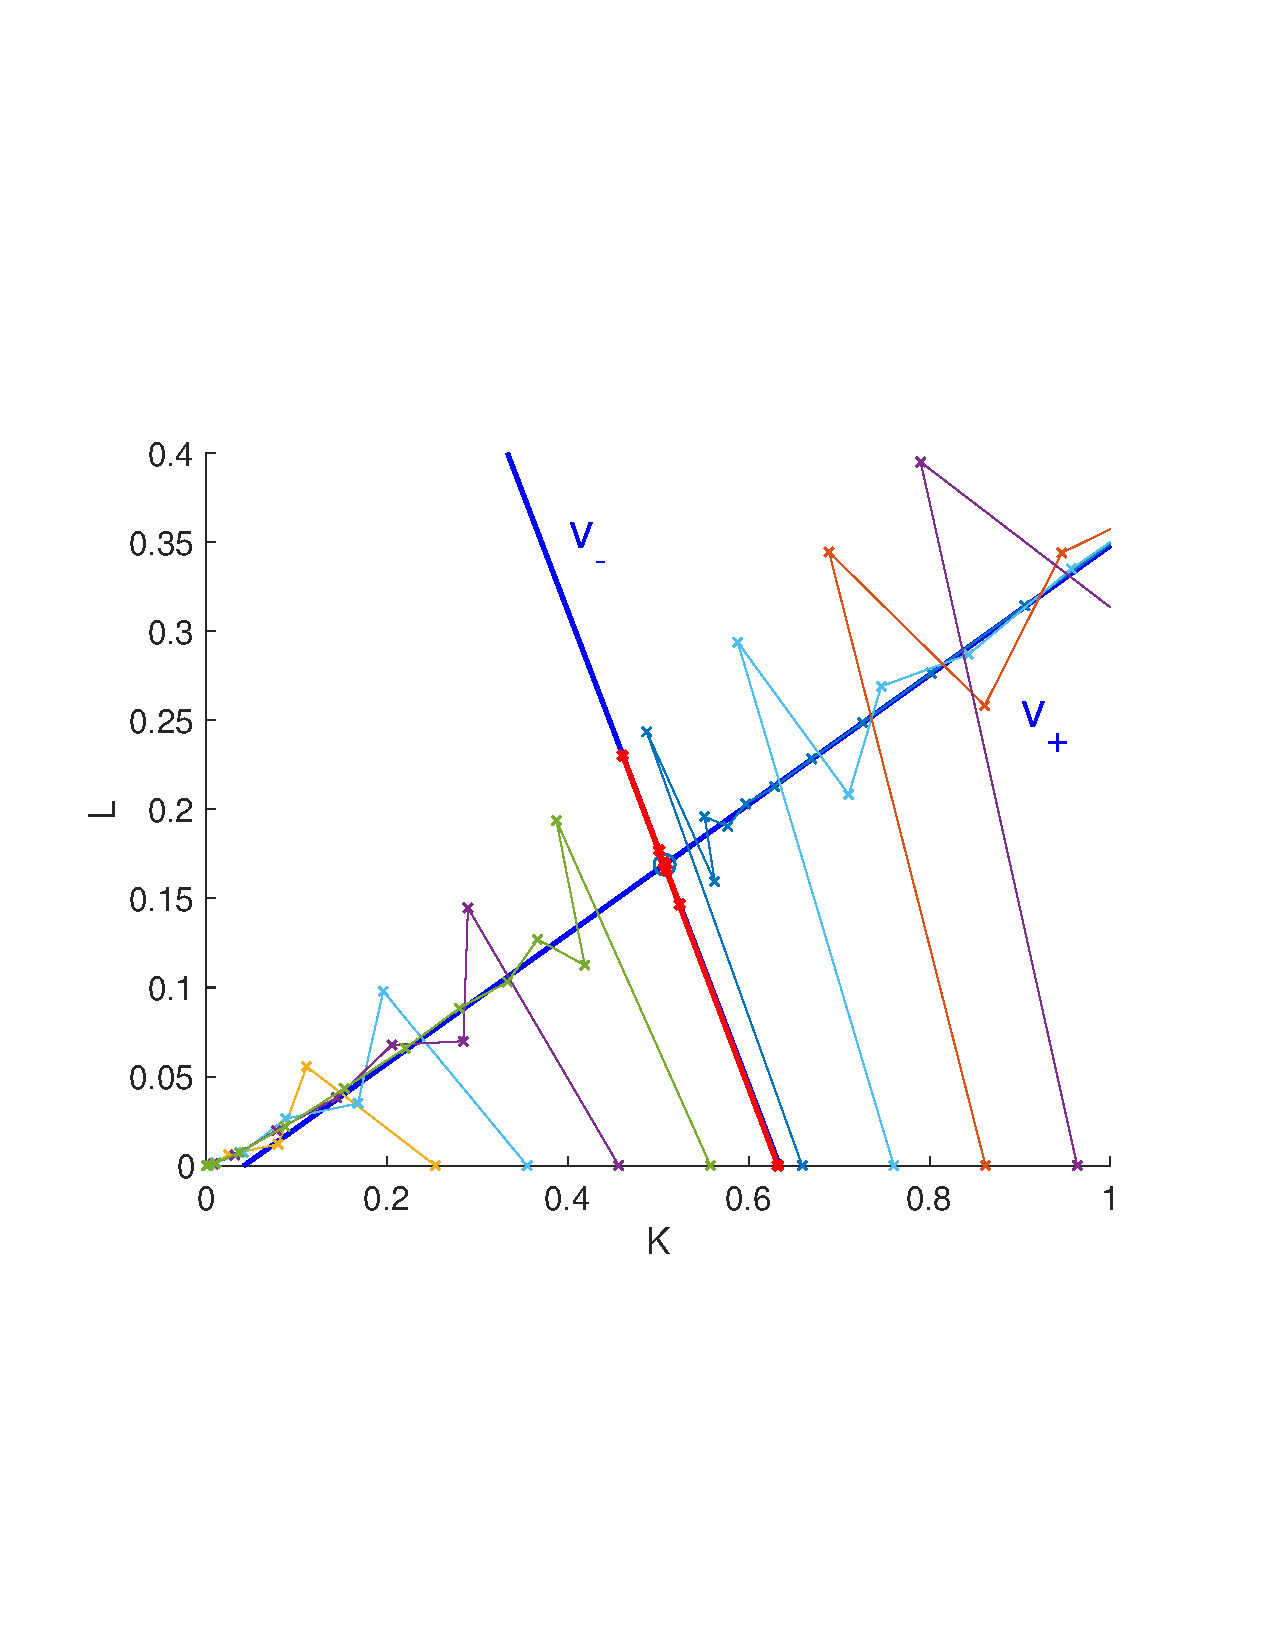
\includegraphics[width=7cm]{RRG_trajectory}
\caption{\bf Flux of the renormalization iterations in the second approximation
described by equation (\ref{eq:RG:Ising:2D:b}). 
All trajectories start at the physical values  $(K,0)$.
The blue solid lines represent the 
principle axes: $\vv x = \vv x^{*} + \lambda \vv v_{\pm}$. The red trajectory is obtained
when starting from $(K_{cr},0)$. Here $K_{cr}$ is chosen as follows: initially  $(K_{cr},0)
=(K^{*},L^{*}) + \eta \vv v_{-}$.   $\eta$ is chosen to fulfil the initial $L=0$ value.
}
\label{fig:rng:ising:2d:b}
\end{center}
\end{figure}

\subsubsection{Taylor expansion}

Often the RG-equation is approximated by assuming small parameters and employing only the 
leading order terms of the Taylor expansion about parameter values equal zero.

The Taylor expansion of $\frac{1}{8} \ln(\cosh(4x))$ gives
%
\begin{align*}
\frac{1}{8} \ln(\cosh(4x)) &= \frac{1}{8} \ln( 1 + \frac{(4x)^{2}}{2} +\ldots  )  = \frac{1}{8} \frac{(4x)^{2}}{2} + \ldots = x^{2}
\end{align*}
%
Then we obtain
%
\begin{align*}
\mqty(K^{*}\\L^{*})
&=
\mqty(
2 {K^{*}}^{2} & L^{*}\\
{K^{*}}^{2}&0
)
\end{align*}
%
with
%$
\begin{align*}
K^{*} &= 3 {K^{*}}^{2}\Rightarrow\qquad K^{*}=1/3\\
L^{*} &= 1/9
\end{align*}
%
In this case the critical value,  obtained numerically, reads $K_{cr} = 0.3921$. That is the K-value used for the initial point $(K,L=0)$ that separates the behaviour whether the trajectories converge towards $(0,0)$
or diverge. 

\begin{comment}

%
\begin{align*}
\mqty(\var K'\\\var L')
&=
\mqty(
4 K^{*} & 1\\
2 K^{*}&0
)
\mqty(\var K\\\var L)
=
\mqty(
\frac{4}{3} & 1\\
\frac{2}{3}&0
)
\mqty(\var K\\\var L)
\end{align*}
%

\end{comment}

%\begin{comment}

 
%



\section{Scaling and critical exponents}

To illustrate this idea we consider again the first approximation (ignoring the nnn
iterations). The iteration equation  was given in
\eq{eq:RG:2D:first} by
%
\begin{align*}
K' &= \frac{3}{8} \ln\qty( \cosh(4K)  ) := R(K)\;:
\end{align*}
%
We consider recursion steps in the vicinity of the fixed point.
We start out from the recursion relation for $K = K^{*}+\var K$
%
\begin{align*}
K' &= R(K) =R(K^{*}) + \underbrace{
\eval{\frac{d}{dK} R(K)}_{K=K^{*}}
}_{\color{blue} = \lambda}\;\var K\\
\Rightarrow\qquad \var K' &= \lambda \var K\;.
\end{align*}
%
The derivative yields
\begin{align}\label{eq:lambda}
\lambda &= \frac{3}{2} \tanh(4 K^{*}) = 1.4489\;.
\end{align}
%
In the present decimation scheme the length is scaled by $b=\sqrt{2}$. 
If we choose a different decimation factor $b$ also $\lambda$ will change, i.e.
%
\begin{align*}
\lambda &= \lambda(b)\;.
\end{align*}
%
When we perform 2 successive decimation steps  we have 
%
\begin{align*}
\var K'' &=\lambda(b) \var K' = \qty(\lambda(b))^{2} \var K\;.
\end{align*}
%
On the other hand, we could have performed the two decimation steps as one combined step of a new decimation scheme with $b'=b\cdot b$, then
%
\begin{align}
\var K'' &=\lambda(b') \var K\;,\nonumber \\
\Rightarrow\qquad \lambda(b^{2}) &= \lambda^{2}(b)\;\label{eq:RG:b}
\end{align}
%
The last equation requires
%
\begin{align*}
\lambda(b) &= b^{y}\;,
\end{align*}
%
where $y$ is a parameter that depends on the underlying physical system but not on $b$;
otherwise \eq{eq:RG:b} would not hold. For the present decimation scheme $b=\sqrt{2}$ and 
$\lambda=1.4489$ (see \eq{eq:lambda}), resulting in 
%
\begin{align*}
y &= \frac{\ln(\lambda)}{\ln(\sqrt{2})} = 1.070\;.
\end{align*}
%


\subsubsection{Correlation length}
We have

%
\begin{align*}
\var K &= K - K_{c} = \frac{J}{k_{B} } \qty(\frac{1}{T} - \frac{1}{T_{c}})
= \frac{J}{k_{B} T} \qty(\frac{T_{c}-T}{T_{c}}) = K \varepsilon \approx K_{c} \varepsilon\;.
\end{align*}
%
From the relation
%
\begin{align*}
\var K' &= b^{y} \var K
\end{align*}
%
we obtain
\begin{align}\label{eq:epsilon}
\varepsilon' &= b^{y} \varepsilon\;.
%\text{or rather } {\varepsilon'}^{-\nu} &= b^{- \nu y} \varepsilon^{-\nu}\;.
\end{align}
%
Moreover, close to $T_{C}$ we have generally
%
\begin{align*}
\frac{\xi}{a} &\sim \varepsilon^{-\nu}
\end{align*}
%
and in the decimated system similarly
%
\begin{align*}
\frac{\xi'}{a'} &\sim {\varepsilon'}^{-\nu}\;,
\end{align*}
%
where $a$ and $a'$ is the lattice constant in the corresponding system.
Then \eq{eq:epsilon} yields
%
\begin{align*}
\frac{\xi'}{a'} &\sim  {\varepsilon'}^{-\nu} =  b^{-\nu y}\;\varepsilon^{-\nu}\sim   b^{-\nu y}\;\frac{\xi}{a}\\
\Rightarrow\qquad \xi' &=  \underbrace{
\frac{a'}{a}
}_{\color{blue} = b (def.)} b^{- \nu y} \;\xi\\
\xi' &= b^{1 - \nu y} \;\xi\;.
\end{align*}
%
On the other hand, on approaching the fixed point the correlation length is converged and does not change. I.e.
%
\begin{align*}
\xi^{*} &= b^{1 - \nu y} \;\xi^{*}\;.
\end{align*}
%
Hence,
%
\begin{align*}
\nu y  &= 1\\
\nu &= \frac{1}{y} = 0.9346\;.
\end{align*}
%
Compared to the exact result ($\nu=1$) for the critical exponent the RG result is not so bad.




\subsubsection{Free energy and specific heat (a bit tricky, will be discussed later)}



Next we want to compute the critical exponent of the specific heat from the free energy 
%
\begin{align}\label{eq:CV:a}
C_{V} &= -T \eval{\pdv{F}{T}}_{V}\;.
\end{align}
%
For the critical exponent which is introduced in  \eq{eq:heat:capacity} as
%
\begin{align*}
C_{V}&\simeq  \abs{\varepsilon}^{-\alpha}
\end{align*}
%
we only need the close neighbourhood of the phase transition.
Hence the factor $T$ in \eq{eq:CV:a} can be replaced by $T_{C}$.
Moreover, we have
%
\begin{align*}
F &= - k_{B} T N \underbrace{
\frac{\ln(Z(K,N))}{N}
}_{\color{blue} := f(K,N)}\;.
\end{align*}
%
Also here the prefactor $T$ can be replace by $T_{C}$ as it does not modify the critical behaviour. So we have
%
\begin{align*}
C_{V} &\sim \pdv[2]{f}{T} \sim |\varepsilon|^{-\alpha}\;.
\end{align*}
%
We recall
%
\begin{align*}
\varepsilon &= \frac{T-T_{C}}{T_{C}}\;,
\end{align*}
%
which yields $f(\varepsilon,N)$ has to have the following behaviour near the phase transition
 %
\begin{align}
\pdv[2]f(\varepsilon,N) &\sim |\varepsilon|^{-\alpha}\nonumber\\
\Rightarrow\qquad f(\varepsilon,N) &\sim |\varepsilon|^{2 -\alpha}\;.
\label{eq:f:epsilon}
\end{align}
%
The integration would also yield a contribution $c + d \;\varepsilon$, which is, however, irrelevant for the critical behaviour.


Next we need to compute $f$.
We start out with the partition function  in the physical parameters 
%
\begin{align*}
Z(K,N) &= \sum_{\{S_{i}\}_{i=1}^{N}} e^{K \sum_{\avg{ij}} S_{i}S_{j}}\;.
\end{align*}
%
After one decimation we have 
%
\begin{align*}
Z(K,N) &= e^{\Delta a N } \sum_{\{S_{i}\}_{i=1}^{N/2}} e^{K' \sum_{\avg{ij}} S_{i}S_{j}}
= e^{\Delta a N } Z(K',N/2)\;.
\end{align*}
%
For the quantity $f(K) := \ln(Z(K,N))/N$ we obtain
%
\begin{align*}
f(K,N) &= \frac{\ln(Z(K,N))}{N} \\
&=\frac{\Delta a N + \ln(Z(K',N/2))}{N}\\
&=\Delta a +  \frac{1}{2} \underbrace{
\frac{\ln(Z(K',N/2))}{N/2}
}_{\color{blue} = f(K',N/2)}
\end{align*}




% 
Since $F=-k_{B} T \ln(Z)$  is an extensive quantity, $f(K,N)$ is independent 
of $N$. So we have
%
\begin{align*}
f(K) &= \Delta a + \frac{1}{2} f(K')\\
f(K') &= 2 f(K) -\Delta a
\end{align*}
%
Inserting \eq{eq:Delta:a} yields
\begin{align}\label{a}
f(K') &= 2 f(K) -   \ln(2 \cosh^{\frac{1}{2}}(2K)\cosh^{\frac{1}{8}}[4 K]) \;.
\end{align}
The second term is analytic and cannot lead to a critical behaviour. The only relevant, singular part $f_{s}$ behaves like
%
\begin{align*}
f_{s}(K') &= 2 f_{s}(K) = b^{d} f_{s}(K)\;.
\end{align*}
%
The scaling factor $b=\sqrt{2}$ and the spatial dimension is $d=2$. Or rather
%
\begin{align*}
f_{s}(K) &= b^{-d} f_{s}(K')\;.
\end{align*}
%
Close to the phase transition we have 
%
\begin{align*}
K &= K^{*} +\var K\\
K' &=  R(K^{*}) +\underbrace{
 \eval{\dv{R(K)}{K}}_{K=K^{*}}
}_{\color{blue} = \lambda}\;\var K\\
\var K' &= \lambda \;\var K
\end{align*}
%
As discussed before we have $\lambda=b^{-y}$ and hence
%
\begin{align*}
\var K' &= b^{y} \;\var K = b^{y} K^{*} \varepsilon
\end{align*}
%
So we have
%
\begin{align*}
f_{s}(K) &= b^{-d}\;f_{s}(K^{*} + b^{y} K^{*} \varepsilon)\\
 &= b^{-d}\;f_{s}(K^{*}[1 + b^{y}  \varepsilon])\;.
\end{align*}
%
This relation has to be valid for any decimation scheme, or rather $b$; so we can choose
%
\begin{align*}
b &= |\varepsilon|^{-1/y}
\end{align*}
%
resulting in 
%
\begin{align*}
f_{s}(K) &= b^{-d}\;f_{s}(K^{*} + b^{y} K^{*} \varepsilon)\\
 &= |\varepsilon|^{d/y}\;\underbrace{
f_{s}(K^{*}[1 +  \frac{\varepsilon}{|\varepsilon|}])
}_{\color{blue} = const}\;.
\end{align*}
%
So we have
%
\begin{align*}
f(\varepsilon,N)&\sim  |\varepsilon|^{d/y}\;.
\end{align*}
%
Comparison with \eq{eq:f:epsilon} yields
%
\begin{align*}
2 - \alpha &= \frac{d}{y}\\
\alpha &= 2 - \frac{d}{y}\;.
\end{align*}
%
Inserting the numerical value from \eq{} gives
%
\begin{align*}
\alpha &= 0.131\;.
\end{align*}
%
The exact value is $\alpha=0$ corresponding  to a logarithmic divergency.
While the mean field result of \eq{spec:heat:MFA} gave constant specific heat 
when approach from below $T_{C}$ and $C_{V}=0$ above $T_{C}$.


%\chapter{Percolation}
%commented out Feb 2024



	 
\chapter{Phase transitions}
\newcommand{\Nphases}{n_{p}}
\section{Phases}
We can generalise  the formalism introduced in statistical physics to incorporate different coexisting phases.

\subsection{Isolated systems}

We begin with isolated systems, where the total volume, total  energy, and the particle number per component is conserved. Let's assume that there are $\Nphases $ coexisting phases, which we enumerate by
($\nu=1,\ldots,\Nphases $) and $\alpha$ components, enumerated by ($j=1,\ldots,\alpha$).
The conditions for isolated systems are therefore
\begin{subequations}\label{eq:constraints}
\begin{align}
\sum_{\nu=1}^{\Nphases } V_{\nu} &= V\\
\sum_{\nu=1}^{\Nphases } U_{\nu} &= U\\
\sum_{\nu=1}^{\Nphases } N_{j\nu} &= N_{j}\;,\text{for } j=1,\ldots, \alpha\;.
\label{eq:constraints:c}
\end{align}
\end{subequations}
Here $V_{\nu}$ ($U_{\nu}$) is the total volume (energy) of the  particles in phase $\nu$.
$N_{j}$ is the total number of particles of component $j$ and $N_{j\nu}$ the number of component
$j$ that is in phase $\nu$. We also introduce the following vectors
%
\begin{align}\label{def:N}
\vv N &= (N_{j=1},N_{j=2},\ldots,N_{\alpha})^{T}\\
\vv N_{\nu} &= (N_{j=1,\nu},N_{j=2,\nu},\ldots,N_{\alpha,\nu})^{T}\;.
\end{align}
%
The entropy as extensive quantity is 
%
\begin{align}\label{eq:}
S(U,V,\vv N) &= \sum_{\nu=1}^{\Nphases } S_{\nu}(U_{\nu},V_{\nu},\vv N_{\nu})\;.
\end{align}
%
For an isolated system (micro-canonical ensemble) the entropy represents the thermodynamic
potential and in equilibrium it has to be maximal. So we have to maximize the entropy based on
the constraints in \eq{eq:constraints}. This is best achieved by Lagrange multipliers, i.e. we define
%
\begin{align}\label{eq:}
{\cal L} &= \sum_{\nu} S_{\nu}(U_{\nu},V_{\nu},\vv N_{\nu})
-\lambda^{V} \sum_{\nu} V_{\nu}
-\lambda^{U} \sum_{\nu} U_{\nu}
-\sum_{j}\lambda^{N}_{j}\sum_{\nu} N_{j\nu}
\end{align}
%
and form the differential
\begin{subequations}\label{eq:}
\begin{align}
d{\cal L} &= \sum_{\nu=1}^{\Nphases } 
\bigg[\frac{\partial }{\partial U_{\nu}}S_{\nu}(U_{\nu},V_{\nu},\vv N_{\nu})\at_{V_{\nu},\vv N_{\nu}} -\lambda^{U}\bigg]dU_{\nu}\\
&\quad +\sum_{\nu=1}^{\Nphases } \bigg[\frac{\partial }{\partial V_{\nu}}S_{\nu}(U_{\nu},V_{\nu},\vv N_{\nu})\at_{U_{\nu},\vv N_{\nu}} -\lambda^{V}\bigg]dV_{\nu}\\
&\quad +\sum_{\nu=1}^{\Nphases } \sum_{j=1}^{\alpha}\bigg[\frac{\partial }{\partial N_{j\nu}}S_{\nu}(U_{\nu},V_{\nu},\vv N_{\nu}) \at_{U_{\nu},V_{\nu},N_{i\nu},i\ne j}-\lambda^{N}_{j}\bigg]dN_{j\nu}
\overset{!}{=}0\;.
\end{align}
\end{subequations}
%
First of all, the variations in volume, energy, and particle number are independent from each other
and, therefore, we have the individual conditions
\begin{subequations}\label{eq:constraint:2}
\begin{align}
\label{eq:constraint:2a}
\sum_{\nu=1}^{\Nphases } 
\bigg[\frac{\partial }{\partial U_{\nu}}S_{\nu}(U_{\nu},V_{\nu},\vv N_{\nu}) \at_{U_{\nu},\vv N_{\nu}}-\lambda^{U}\bigg]dU_{\nu}&=0\\
\sum_{\nu=1}^{\Nphases } \bigg[\frac{\partial }{\partial V_{\nu}}S_{\nu}(U_{\nu},V_{\nu},\vv N_{\nu})\at_{V_{\nu},\vv N_{\nu}} -\lambda^{V}\bigg]dV_{\nu} &=0\\
\sum_{\nu=1}^{\Nphases } \sum_{j=1}^{\alpha} \bigg[\frac{\partial }{\partial N_{j\nu}}S_{\nu}(U_{\nu},V_{\nu},\vv N_{\nu})\at_{U_{\nu},V_{\nu},N_{i\nu},i\ne j} -\lambda^{N}_{j}\bigg]dN_{j\nu} &=0\;.
\end{align}
\end{subequations}
According to the constraints \eq{eq:constraints}, there is one condition for the variables $U_{\nu}$, i.e. we can choose $U_{\nu}$ for $\nu=1,2,\ldots,\Nphases -1$ as we like and $U_{\Nphases }$
follows from the constraint. Then we can always choose
%
\begin{align}\label{eq:constr:nu}
\lambda^{U} &=\frac{\partial }{\partial U_{\Nphases }}
S_{\Nphases }(U_{\Nphases },V_{\Nphases },\vv N_{\Nphases })\at_{U_{\Nphases },\red{\vv N_{\Nphases } }} \;,
\end{align}
as long as we are eventually able to fulfil the constraint \eq{eq:constraint:2a}.
Then the remaining constraint reads
%
\begin{align*}
\sum_{\nu=1}^{\Nphases -1} 
\bigg[\frac{\partial }{\partial U_{\nu}}S_{\nu}(U_{\nu},V_{\nu},\vv N_{\nu})\at_{V_{\nu},\vv N_{\nu}} -\lambda^{U}\bigg]dU_{\nu}&=0;.
\end{align*}
%
Here all $dU_{\nu}$ are independent and the square brackets have to vanish individually. Then we have for all $\nu$ (the last comes from \eq{eq:constr:nu})
\begin{subequations}
\begin{align}
\lambda^{U}&=\frac{\partial }{\partial U_{\nu}}S_{\nu}(U_{\nu},V_{\nu},\vv N_{\nu})\at_{V_{\nu},\vv N_{\nu}} &&= \frac{1}{T_{\nu}}\;.
%
\intertext{Similarly, we obtain from the other constraints}
%
\lambda^{V}&=\frac{\partial }{\partial V_{\nu}}S_{\nu}(U_{\nu},V_{\nu},\vv N_{\nu})\at_{U_{\nu},\vv N_{\nu}} &&=\frac{p_{\nu}}{T_{\nu}}\;.
\intertext{and}
%
\lambda_{j}^{N} &=
\frac{\partial}  {\partial N_{j\nu}}
S_{\nu}(U_{\nu},V_{\nu},\vv N_{\nu})\at_{U_{\nu},V_{\nu},N_{i\nu},i\ne j}
&&=-\frac{\mu_{j\nu}}{T_{\nu}}\;,\qquad\text{for } j= 1,\ldots,\alpha\;.
\end{align}
\end{subequations}
Since the Laplace multipliers on the lhs of these equations are independent of $\nu$,
we find that in an isolated system in equilibrium all phases have the same temperature $T$,
the same pressure $p$ and the same chemical potential $\mu_{j}$ for component $j$. But in general, we still have  $\mu_{j}\ne \mu_{j'}$: The chemical potential in the different phases of one component is equal, but the chemical potential of the different components must not be equal.

\tboxit{State variables in different phases }{
%
\begin{subequations}\label{eq:state:var:phases}
\begin{align}
T_{\nu} &= T\;&&\forall  \nu\\
p_{\nu} &= p\;&&\forall  \nu\\
\mu_{j,\nu} &= \mu_{j}\;&&\forall  \nu\;.
\end{align}
\end{subequations}%
}
\subsection{Closed system with $p=fixed$, $T=fixed$}

Another important system is that where pressure and temperature are fixed experimentally.
In this case the  Free Enthalphy $G(p,T,\vv N)$ is the relevant thermodynamic potential.
The equilibrium condition is $G$ has to be minimal, or rather $dG=0$. Again $G$ is extensive, i.e.
additive w.r.t. the phases
%
\begin{align}\label{eq:}
G &= \sum_{\nu=1}^{\Nphases } G_{\nu}(T,p,\vv N_{\nu})
\end{align}
%
Here, we have already exploited that all phases have the same temperature and pressure, which is given at the outset. So the only degree of freedom that can be varied are the particle numbers, still under the constrain used before. A similar derivation now yields
%
\begin{align}\label{eq:mu:condition}
\lambda^{N}_{j}&=\frac{\partial }{\partial N_{j\nu}} G_{\nu}(T,p,\vv N_{\nu})\at_{T,p,N_{i,\nu},i\ne j} = \mu_{j,\nu}\;.
\end{align}
%
and we find that in a closed system, where $T$ and $p$ is fixed, the chemical potential of component
$j$ is the same in all phases.
\subsection{Number of degrees of freedom}
The chemical potentials will depend on $T$, $p$, and in principle on the particle numbers
%
\begin{align}\label{eq:}
\mu_{j\nu} &=\mu_{j\nu}(T,p,\{N_{j\nu}\})
\end{align}
%
Now, the chemical potentials are intensive quantities, i.e. scaling the extensive quantities in its argument, by a common factor does not change the chemical potential. Let's consider an intensive function
$f$ that shall depend on $T$, $p$, and some particle numbers $N_{l}$. Scaling the total size
by $\lambda$ results in particle numbers $\lambda N_{l}$. As $T$ and $p$ are intensive,
we have 
%
\begin{align*}
f(T,p,\{\lambda N_{l}\}) &= f(T,p,\{N_{l}\})\;.
\end{align*}
%
This is the case if $f$ only depends on the concentrations $c_{j}=N_{j}/\sum_{i} N_{i}$, since
scaling all $N_{j}$ by a common factor does not change the concentration.


\begin{enumerate}
	\item By phase we mean a spatial area within which no abrupt changes of any physical quantity occur,
but at the boundary of which such changes can be observed. 
\item The system consists of one or more component/ components. Component means the minimum number
of independent chemical substances that we need to produce the phase.
\item The state of the system is described by a number of state variables depending on the type of system. 
\item By degrees of freedom F we mean the number of state variables that we can vary independently of 
each other without any of the phases disappearing. 


\item First of all, we want to assume that no chemical reactions take place in the system. 
The state of each phase is clearly defined when we specify $T$, $p$, and the mole fraction of component $j$ in phase $\nu$.
%
\begin{align}\label{eq:}
c^{(\nu)}_{j} &:= \frac{N_{j\nu}}{N_{\nu}}\,
\end{align}
%
i.e. the fraction of particles in phase $\nu$ that belong to component $j$.
\end{enumerate}
%
 Then
%
\begin{align}\label{eq:mole:fraction:normalization}
\sum_{j} c^{(\nu)}_{j} &= 1\;,\qquad \forall \nu\;.
\end{align}
% 
Scaling the total size of the system by a common factor $\lambda$, i.e. in particular $N_{j\nu}\to \lambda N_{j\nu}$, does not change the phases. So along with the intensitivity of the chemical potentials, we know by now that the latter depend on the mole fractions and not the absolute particle numbers
%
\begin{align}\label{eq:mu:molefraction}
\mu_{j\nu} &=\mu_{j\nu}(T,p,\{c^{(\nu)}_{j}\})\;.
\end{align}
%
The number of state variables is $Z_{v}=2 + \alpha \Nphases $, but they are not independent.
%
According to \eq{eq:mu:condition} we have the equilibrium conditions, which 
include the conditions for the particle numbers in \eq{eq:constraints:c}
%
\begin{align*}
\mu_{j\nu}(T,p,\{N_{j\nu}\}) &= \mu_{j\nu'}(T,p,\{N_{j\nu}\})\;, \forall \nu\ne \nu'
\text{and } \forall j\;. 
\end{align*}
%
These are $\Nphases -1$ conditions for each component, i.e. in total $\alpha(\Nphases -1)$ constraints.
E.g. for $\Nphases =2$ we have one condition per component $\mu_{j,1}=\mu_{j,2}$.
In addition we have the $\Nphases $ normalization constraints in \eq{eq:mole:fraction:normalization}.
So the total number of constraints is 
%
\begin{align*}
Z_{c} &= \alpha \Nphases -\alpha + \Nphases \;,
\end{align*}
%
and therefore the number of d.o.f. is the number of state variables minus the number of constraints
resulting in 
%
\begin{align*}
f &=\big( \alpha \Nphases +2\big) - \big(\sigma \Nphases -\alpha+\Nphases \big)
\end{align*}
%
%
\tboxit{Gibbs' phase rule}{
\begin{align}
f &=  2 + \alpha - \Nphases \;.
\end{align}}
%

\subsubsection{Example: $H_{2}O$ Phase diagram}
\begin{figure}[htbp]
\begin{center}
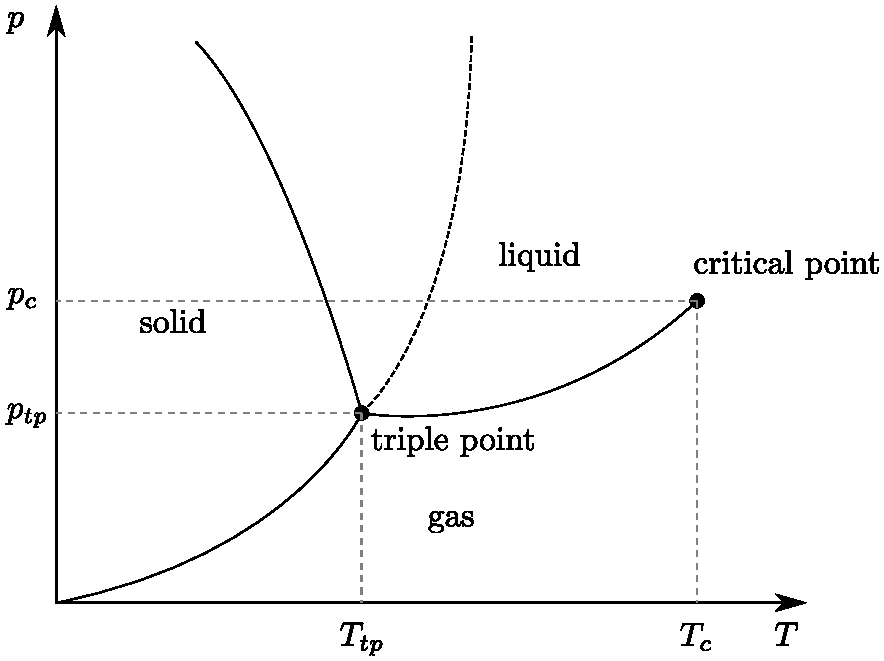
\includegraphics[width=0.8\textwidth]{water_phase_transitions.pdf}
\caption{Schematic phase diagram for water. Note that the slope of the transition line from solid to liquid has a negative slope. The dashed line corresponds to the transition from solid to liquid for most other substances and shows a positive slope.}
\label{fig:water:phasediagram}
%TODO: change this figure to either self-made figure or some copyright-free image
\end{center}
\end{figure}

In \autoref{fig:water:phasediagram} the phase diagram of water is shown. The lines in this diagram indicate the conditions of pressure and temperature, where a phase transition can happen - in the areas between the lines, water exists only in the corresponding phase. 

\begin{itemize}
	\item 
		triple point: $T_{tp}=273.16000 ~\text{K} ~(0.01000 ~\text{°C})$, $p_{tp}=611.657 ~\text{Pa}$. \\
		All three phases can coexist at these conditions
	\item
		critical point: $T_{c} = 647.096 ~\text{K}$, $p_{c} = 22.064 ~\text{MPa}$ and $\rho_{c} = 356 ~\text{kg/m}^{3}$. \\
		Past this point, the phase transition between gaseous and liquid water vanishes.
	\item 
		transition solid $\leftrightarrow$ liquid: melting, freezing 
 	\item 
		transition liquid $\leftrightarrow$ gas:  vaporization, condensation
 	\item 
		transition solid $\leftrightarrow$ gas: sublimation, deposition
\end{itemize}

What is interesting about water is the phase transition between solid and liquid phase. Contrary to other chemical substances, the line corresponding to this transition in the phase diagram has a negative slope. When we increase the temperature, the pressure, at which the transition happens decreases or phrased in a more intuitive way: The density of ice is smaller than the density of water. What we would normally expect would be a decrease of density when the temperature rises but apparently, water behaves differently. This effect is called the anomaly of water and it is the reason why ice floats on water and why  creatures living in water  survive in winter.

Water is a one component liquid, i.e. $\alpha=1$, in the following we will consider the different areas of the phase diagram where different phases coexist:

\subsubsection{a) Pure phases (solid,liquid,gas), $\Nphases =1$}

The number of degrees of freedom is, according to Gibb's phase rule, 
%
\begin{align*}
f = 2 + \alpha -\Nphases  = 2 + 1 - 1 = 2\;,
\end{align*}
%
which means we can vary to state variables, here $T$ and $p$, independently.

\subsubsection{b) Two coexisting phases, $\Nphases =2$}
\begin{itemize}
   \item boiling curve (liquid to gas)
 \item condensation curve (gas to liquid)
	\item melting curve (solid to liquid)
 \item solidification curve (liquid to solid)

\item sublimation curve (solid to gas)
\item resublimation curve (gas to solid)
	
\end{itemize}


The number of degrees of freedom is 
%
\begin{align*}
f = 2 + 1 - 2 = 1\;,
\end{align*}
%
which means, we have to vary  $T$ and $p$ on a curve, $p(T)$, e.g. melting-point line.



\subsubsection{c) Three coexisting phases, $\Nphases =3$, triple point}

Here $f=0$. There is no degree of freedom. 

It also follows that for a one-component substance there are at most 3 phases, otherwise the
number of degrees of freedom would become negative.


\subsection{Clausius-Clapeyron}

As a further application of the previous discussion, we consider the coexistence line between
liquid and gas (Condensation curve) of a one-component system, such as water. 

If we choose $T$ and $P$ as the two independent d.o.f. then according to 
\eq{eq:mu:condition} we have
%
\begin{align}\label{eq:mu:coexist}
\mu_{fl}(T,p) &= \mu_{g}(T,p)\;.
\end{align}
%
This relation allows to determine to condensation curve $p(T)$ on which the fluid and the gas phase coexist. Away from this curve, only one phase exists, namely the one where the chemical potential is smaller. This is due to the Gibbs-Duhem relation for the free Enthalpy
%
\begin{align*}
G(T,p,N) &= \mu N\;.
\end{align*}
% 
In the case of a single phase, the system will minimize the Free Enthalpy $G$. Since $N$ is fixed,
the phase with  the smaller chemical potential has a smaller Free Enthalpy.

The free Enthalpy is related to the free energy $F(T,V,N)$ via a Legendre transformation,
where $V$ is replaced by $p$. We start out with
%
\begin{align*}
\frac{\partial }{\partial V} F(T,V,N)\at_{T,N} &= - p
\end{align*}
%
This relation can be inverted for given $T,N$ and $p$ we obtain
%
\begin{align*}
V &=V(p,T,N)
\end{align*}
%
%
\begin{align}
G(T,p,N) &= F(T,V(p,T,N),N) + p V\;.
\end{align}
%
Then
%
\begin{align*}
dG &= dF +pdV + Vdp\\
&= -SdT -p dV +\mu dN +pdV + Vdp\;.
\end{align*}
%
Hence  we have
%
\begin{align*}
dG &= \mu dN - S dT + V dp\;,
\intertext{or rather}
dG - \mu dN &= - S dT + V dp\;.
\end{align*}
%
On the other hand the Gibbs-Duhem relation yields
%
\begin{align*}
dG &= \mu  dN + N d\mu\Rightarrow dG - \mu dN = N d\mu\;.
\end{align*}
%
Combining the two relation yields
%
\begin{align*}
- S dT + V dp &= N d\mu\;.
\end{align*}
%
This is generally valid and it also applies individually to different phases, which here shall
have the same $T$ and $p$, i.e.
\begin{align*}
- S_{\nu} dT + V_{\nu} dp &= N_{\nu} d\mu_{\nu}\notag\\
- \frac{S_{\nu}}{N_{\nu}} dT + \frac{V_{\nu}}{N_{\nu}} dp &=  d\mu_{\nu}\;.
\end{align*}
We introduce entropy and volume per particle
%
\begin{align}\label{eq:}
s_{\nu} &= \frac{S_{\nu}}{N_{\nu}}\\
v_{\nu} &= \frac{V_{\nu}}{N_{\nu}}\;,
\end{align}
%
and obtain
%
\begin{align}\label{eq:dmu:nu}
- s_{\nu}  dT + v_{\nu} dp &=  d\mu_{\nu}\;.
\end{align}
%
%
%
Now we consider changes $dp,dT$ along the coexistence line.
There we have due to \eq{eq:mu:coexist}
%
\begin{align*}
d\mu_{fl}(T,p) &= d\mu_{g}(T,p)\;.
\end{align*}
%
Along with \eq{eq:dmu:nu} we obtain
\begin{align*}
- s_{fl}  dT + v_{fl} dp &= - s_{g}  dT + v_{g} dp \\
\frac{dp}{dT} &= \frac{s_{g}-s_{fl}}{v_{g}-v_{fl}} = \frac{\Delta s}{\Delta v}\;.
\end{align*}
Finally, we define the molar vaporation enthalpy
%
\begin{align*}
q &= T\big( s_{g}-s_{fl} \big)
\end{align*}
%
and find the
\tboxit{Clausius-Clapeyron relation}{
%
\begin{align}\label{eq:}
\frac{dp}{dT}&= \frac{q}{T\big( v_{g}-v_{fl} \big)}\;.
\end{align}
%
}
In the derivation of the Clausius-Clapeyron relation we have assumed that $ S_{g}\ne S_{fl}$
and $V_{g}\ne V_{fl}$, which means, although 
%
\begin{align*}
\mu_{g}(T,p) &=\mu_{fl}(T,p) 
\end{align*}
%
that
%
\begin{align*}
\frac{\partial \mu_{g}}{\partial T}\at_{p} &\ne \frac{\partial \mu_{fl}}{\partial T}\at_{p}\\
\frac{\partial \mu_{g}}{\partial p}\at_{T} &\ne \frac{\partial \mu_{fl}}{\partial p}\at_{T}\;.
\end{align*}
%
So apparently, the chemical potential $\mu(T)$ is continuous at the temperature of phase transition, but its first derivative is not (i.e. $\mu(T$) is continuous, but not differentiable). Such a phase transition is called a first order phase transition.

Generally, if we have similar behaviour where the the $n$-th derivative of $\mu(T)$ is not continuous, but up until the $(n-1)$-th derivative, they are all continuous, we call this a phase transition of $n$-th order. We will further look at this in \autoref{sec:ehrenfest:classification}. This means that the Clausius-Clapeyron relation is only valid for first order phase transitions.

\subsection{Real gases (van der Waals equation)}
In statistical physics we have discussed the ideal gas and its equation of state

%
\begin{align*}
p V &= N k_{B} T\;.
\end{align*}
%
We also introduced finite eigen-volumes of the moelcules and obtained
%
\begin{align*}
p \big(V- V_{0}\big) &= N k_{B} T\;.
\end{align*}
%
Finally, we also want to include the intermolecular forces. For molecules in the bulk of the 
material, these forces vanish on average, as they act with equal strength in opposite directions.
This is not the case in the surface layer, where the partners outside the surface are missing.
This results in an effective force, pulling the molecules  in the surface layer into the bulk. I.e.
the intermolecular forces act at the surface like an additional pressure (internal pressure).
It has the form 
%
\begin{align*}
a \frac{N^{2}}{V^{2}}
\end{align*}
%
resulting in 
\tboxitp{van der Waals equation}{extensive form}{
%
\begin{align}\label{eq:vdW:ext}
\bigg( p + a' \frac{N^{2}}{V^{2}} \bigg)\bigg(V - \overbrace{N b'}^{V_{0}} \bigg) &= N k_{B} T\;.
\end{align}
%
}
It can also be expressed in terms of molar volume $v$, pressure and temperature, i.e.
the intensive form 
\tboxitp{van der Waals equation}{intensive representation}{
%
\begin{align}\label{eq:vdW:int}
\bigg( p + \frac{a'}{v^{2}} \bigg)\bigg(v - b' \bigg) &= k_{B} T\;.
\end{align}
%
}
Here, $b'$ is the eigen-volume of one molecule.

We multiply \eq{eq:vdW:int} by $v^{2}$ and find that it becomes a cubic equation in $v$
%
\begin{align*}
\bigg( p v^{2}+ a' \bigg)\bigg(v -  b' \bigg) - k_{B} T v^{2}&= 0\\
p v^{3} + a' v   -  b' p v^{2} - a' b' - k_{B} T v^{2}&= 0\;.
\end{align*}
%
Next we introduce suitable units $p_{cr},v_{cr},T_{cr}$ and the corresponding dimensionless 
quantities $\pi,\nu,t$ via
%
\begin{align*}
p &=\pi p_{cr}\\
v &=\nu v_{cr}\\
T &= t T_{cr}\;,
\end{align*}
%
resulting in 
%
\begin{align*}
\pi \nu^{3} + \frac{a' v_{cr}}{p_{cr} v_{cr}^{3} } \nu -\frac{b' p_{cr}  v_{cr}^{2}}{p_{cr} v_{cr}^{3} } \pi \nu^{2}
-\frac{a'b'}{p_{cr} v_{cr}^{3} } - \frac{k_{B}T_{cr} v_{cr}^{2}}{p_{cr} v_{cr}^{3} } t \nu^{2}&=0 \\
\pi \nu^{3} + \underbrace{
\bigg(\frac{a' }{p_{cr} v_{cr}^{2} }\bigg) 
}_{\color{blue} = T_{1}}\nu
 -\underbrace{
\bigg(\frac{b'  }{ v_{cr} }\bigg) 
}_{\color{blue} = T_{2}}\pi \nu^{2}
-\underbrace{
\bigg(\frac{a'b'}{p_{cr} v_{cr}^{3} }\bigg)
}_{\color{blue} = T_{3}} - 
\underbrace{
\bigg(\frac{k_{B}T_{cr} }{p_{cr} v_{cr} } \bigg)
}_{\color{blue} = T_{4}}
t \nu^{2}&=0 \\
\pi \nu^{3} + T_{1}\nu - T_{2} \pi \nu^{2}
-T_{3} - T_{4} t \nu^{2}&=0 \;.
\end{align*}
%
Now we have the freedom to choose the parameters $p_{cr}$, $v_{cr}$, and $T_{cr}$ suitably.
We use
%
\begin{align}
T_{_{2}} &=\bigg(\frac{b'  }{ v_{cr} }\bigg)= \frac{1}{3}\\
T_{3}&= \bigg(\frac{a'b'}{p_{cr} v_{cr}^{3} }\bigg) =1\\
T_{4}&=\bigg(\frac{k_{B}T_{cr} }{p_{cr} v_{cr} } \bigg)= \frac{8}{3}
\end{align}
%
then
\tboxitp{Critical values}{van der Waals}{
\begin{align}\label{def:critical:values}
v_{cr} &= 3 b'\\
\Rightarrow\qquad p_{cr}&= \frac{a'b'}{ v_{cr}^{3} } = \frac{a'}{27b'^{2}}\\
\Rightarrow\qquad T_{1}&= \frac{a'}{p_{cr} v_{cr}^{2}} = \frac{a'}{\frac{a'}{27 b'^{2}}9 b'^{2}} = 3\\
k_{B}T_{cr} &= \frac{8}{3} p_{cr} v_{cr} =\frac{8}{3} \frac{a'}{27 b'^{2}}\;3 b'
=\frac{8 a'}{27 b'}\;.
\end{align}}
%
So we have
%
\begin{align}\label{eq:auxaux}
\pi \nu^{3} + 3 \nu -  \frac{\pi \nu^{2}}{3} - 1 &= \frac{8}{3}t \nu^{2}\\
\bigg( \pi + \frac{3}{\nu^{2}} \bigg)\bigg( \nu - \frac{1}{3} \bigg) &=\frac{8}{3} t\;.
\end{align}
%
Solving for $\pi$ yields
%
\begin{align*}
\pi &= \frac{8t}{3 \nu-1 } - \frac{3}{\nu^{2}}
\end{align*}
%
The term $(3\nu-1)$ originated from $V-V_{0}$, and therefore it is always positive,
as the total volume has to be greater than the eigen volume. 

If we plot $\pi(\nu)$ for fixed $t$ (isotherm) then we find different behaviour for $t<1$, $t=1$ and $t>1$.
%
\begin{figure}[htbp]
\begin{center}
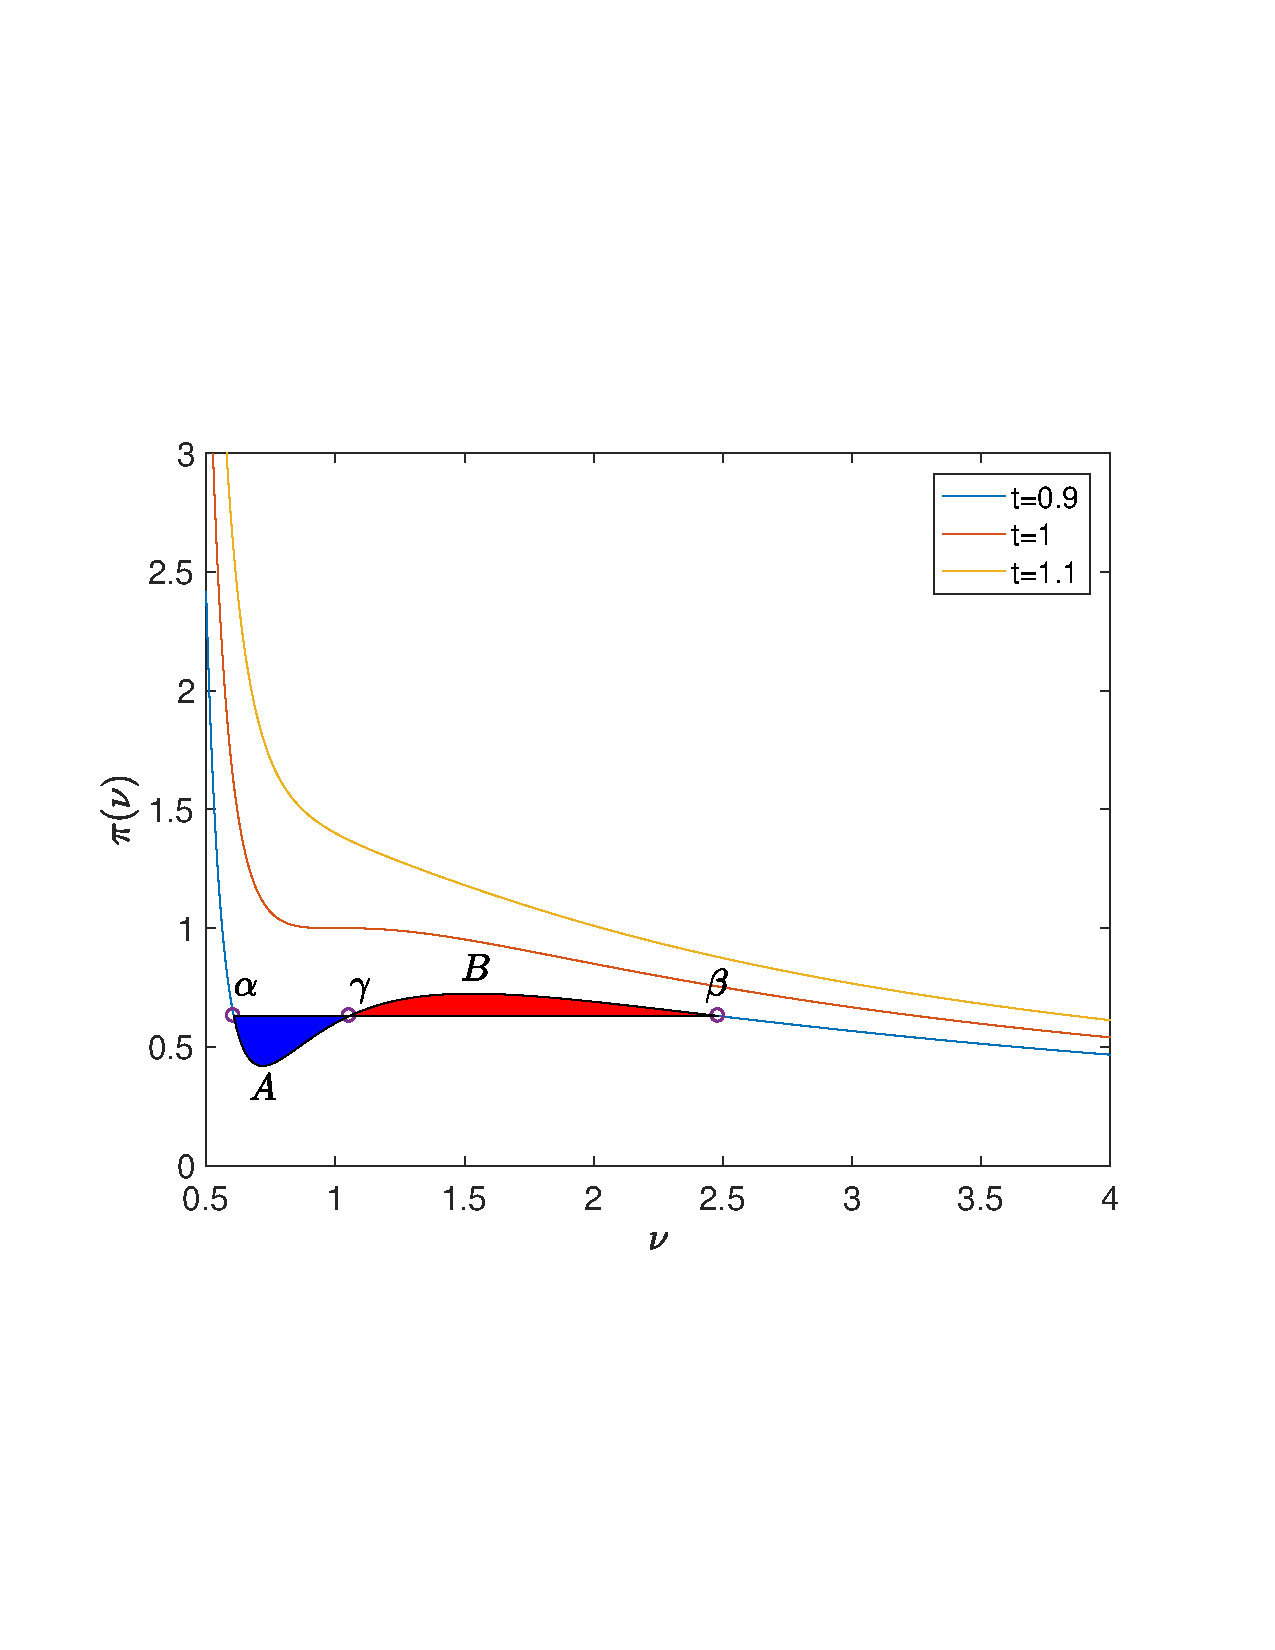
\includegraphics[width=10cm]{Maxwell}
\caption{Different types of isotherms in the $\pi$-$\nu$-diagram and Maxwell construction}
\label{fig:Maxwell:isotherms}
\end{center}
\end{figure}
%
\begin{itemize}
\item For $t<1$ the curve has a minimium and a maximum in the physical interval $\nu>1/3$.
\item For $t=1$ minimum and maximum coincide at $\nu=1$, with $\pi(\nu=1)=1$.
 \item For $t>1$ the curve is monotonically decreasing in the physical interval.
\end{itemize}
We will see soon that there is a phase transition if the curve has a maximum and a minimum.
 If it is monotonically decreasing, there is no phase transition. Hence, the parameters
 $p_{cr}$,  $v_{cr}$, and  $T_{cr}$ represent the  critical point.
 
 
Inserting the critical values into the van-der-Waals equation of state in form of the following ratio
then we obtain
%
\begin{align}\label{def:Z:cr}
Z:=\frac{p_{cr} v_{cr}}{k_{B} T_{cr}} &=  \frac{\frac{a'}{27 b'^{2}}3 b'}{\frac{8 a'}{27 b'}} =
\frac{3}{8}\;.
\end{align}
%
Experimentally one finds for all real gases at the critical point $Z<3/8$, while the ideal gas yields $Z=1$. In this respect the van der Waals model is clearly better.
Alternatively, \eq{def:Z:cr} can be written with $\rho_{c}=1/v_{cr}$ as
%
\begin{align}\label{eq:p:cr}
p_{cr} &=\frac{3}{8} k_{B} T_{cr} \rho_{cr}\;.
\end{align}
%

\subsection{Maxwell-Construction}

We have just seen that the equation of state for the van-der-Waals model reads in dimensionless units
%
\begin{align*}
\bigg( \pi - \frac{3}{\nu^{2}} \bigg)\bigg(\nu  -\frac{1}{3}\bigg) &=\frac{8}{3} t\;,
\end{align*}
%
and that  $t<1$ there   are regions in the $\pi-\nu$-diagramm where the isotherm compressiblility
%
\begin{align}\label{eq:}
\kappa_{T}&= - \frac{1}{V} \bigg(  \frac{\partial V}{\partial p}\at_{T}\bigg)
= - \frac{1}{p_{cr} \nu} \bigg(  \frac{\partial \nu}{\partial \pi}\at_{T}\bigg) <0
\end{align}
%
becomes negative. This implies that the system is mechanically unstable, it would shrink by itself.

\blue{The reason is  that the van der Waals model describes a single phase of a one-component system.}
It is applicable  in the pure gas or  liquid phase (grey shaded areas in the figure),
but in between there is a phase transition, where two phases coexist, which cannot be described by the van-der-Waals equation.
%
\begin{figure}[htbp]
\begin{center}
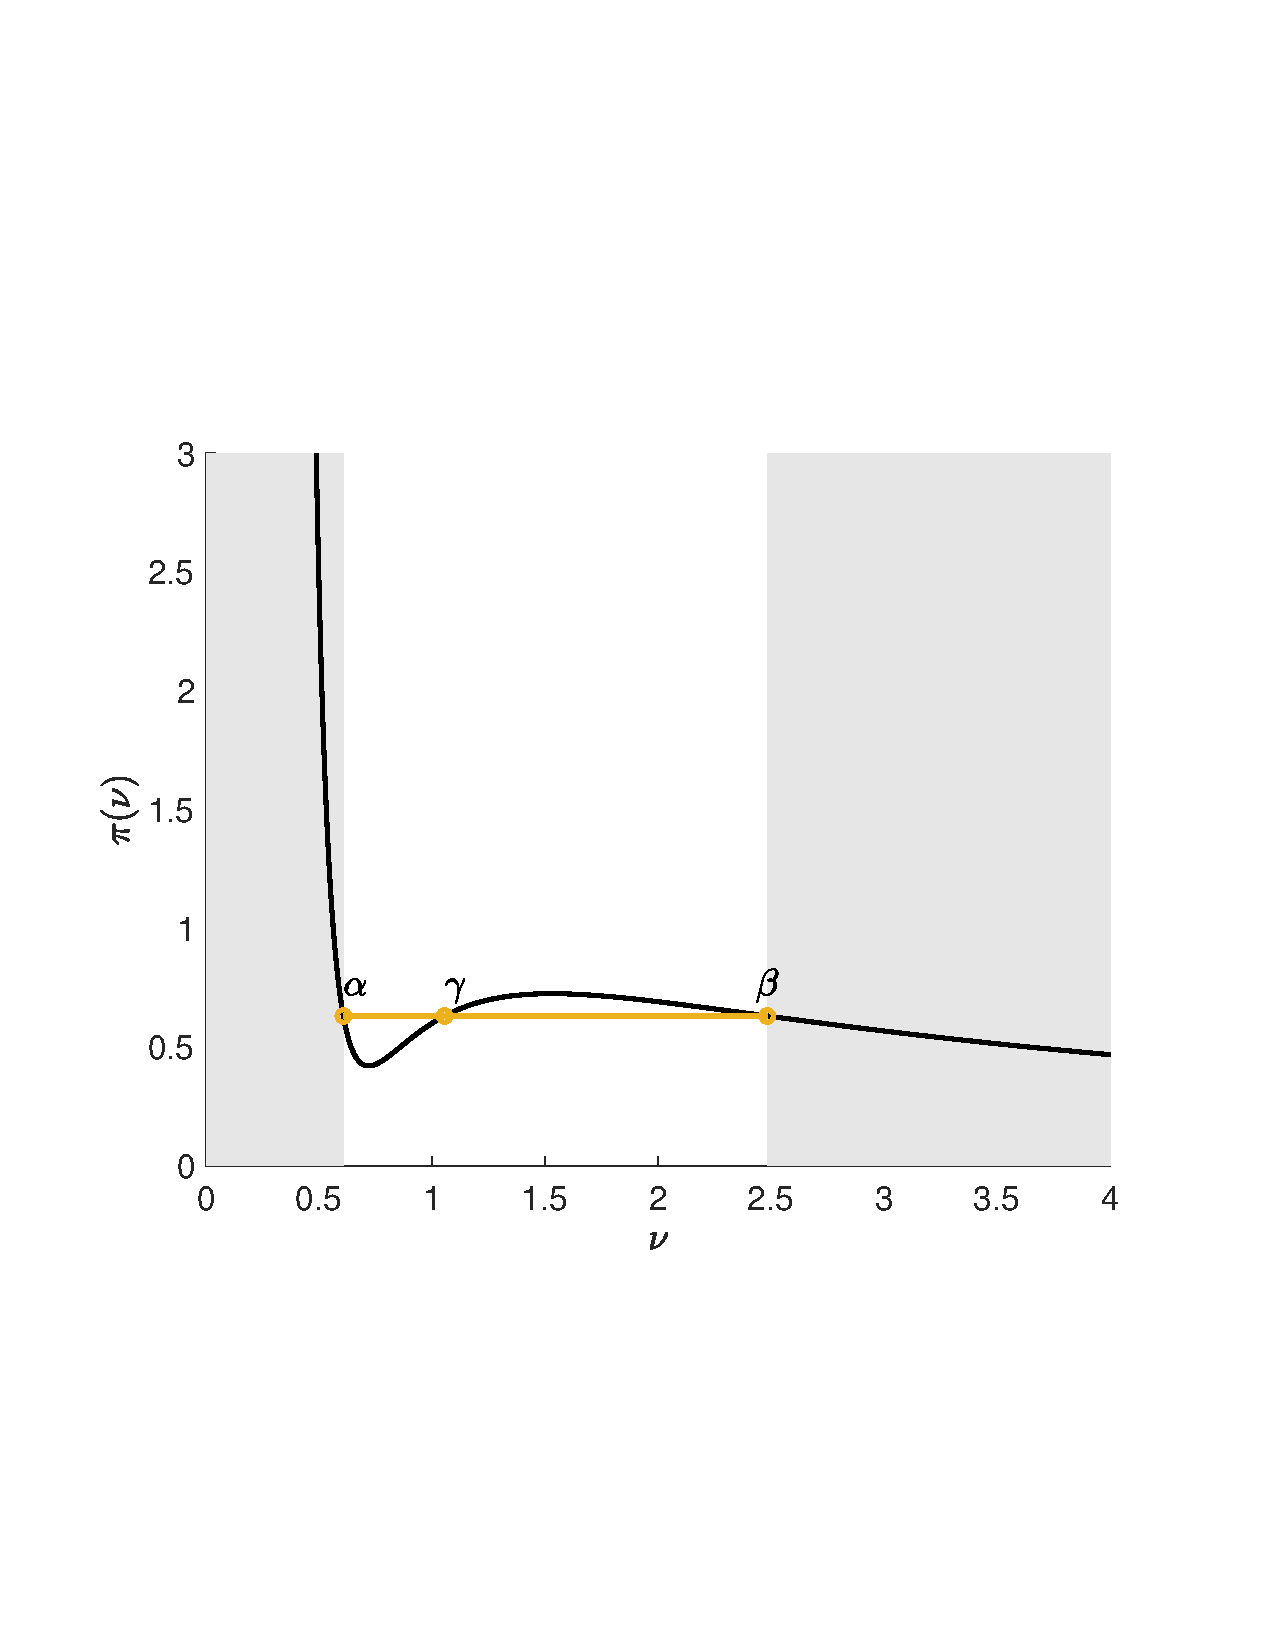
\includegraphics[width=8cm]{Maxwell_new}
\caption{\bf Maxwell construction.}
\label{fig:Maxwell}
\end{center}
\end{figure}
%


What happens in reality is the following. We have seen before that generally on the coexistence 
line between liquid and gas, the number of degrees of freedom is merely 1 and it is described by $p=p(T)$.
On isotherms, $T$ is also fixed and therefore $p$ is fixed as well and takes a constant value.

%
\nboxit{blue}{All isotherms for ($T<T_{c}$) in the two-phase region have to be horizontal lines in the pV-diagram. (See golden line in the \autoref{fig:Maxwell})} 

We denote the pressure on the coexistence line between the points $\alpha$ and $\beta$ in the 
$\pi$-$\nu$-diagram by $p_{\alpha\beta}$.

In the pure phases of a one-component system we have only two degrees of freedom, e.g.
$p$ and $T$.
Since the van-der-Waals model is still valid in the pure phase regions (grey shaded),
we have the condition (\eq{eq:mu:coexist})
%
\begin{align*}
\mu_{fl}(T,p) &= \mu_{g}(T,p)\;.
\end{align*}
%
Hence for the isotherm compression, discussed before, the pressure  ($p_{\alpha\beta}$) when reducing the volume in the two-phase region, does not change and we have
%
\begin{align*}
\mu_{fl}(T,p_{\alpha\beta}) &=\mu_{g}(T,p_{\alpha\beta})\;.
\end{align*}
%
In addition, at the points $\alpha$ and $\beta$, we have pure phases and therefore $N_{\alpha}=N$ and $N_{\beta}=N$ and consequently at the end points of the horizontal line we have
%
\begin{align*}
\mu_{fl}(T,P_{\alpha\beta}) N_{\alpha} &=\mu_{g}(T,P_{\alpha\beta}) N_{\beta}
\end{align*}
%
Then the Gibbs-Duhem relation ($G=\mu N$)  yields for these points
%
\begin{align*}
G_{\alpha} &= G_{\beta}\\
F_{\alpha} + p_{\alpha}V_{\alpha} &=F_{\beta} + p_{\beta} V_{\beta} 
\end{align*}
%
from which we conclude
%
\begin{align}\label{eq:DF:DV}
F_{\alpha}-F_{\beta} &= -p_{\alpha\beta}(V_{\alpha}-V_{\beta})\;.
\end{align}
%
This is the result for the end points of the coexistence line, where we have exploited some of the features of the  two phase region in between, for which we have used $\pi(\nu) = p_{\alpha\beta}$, independent of volume $\nu$.
Alternatively, if we stick to one phase then the van-der-Waals equation determines the pressure curve, the one given in figure \ref{fig:Maxwell:isotherms} with the wavy look.
In that case, the differential of the free energy is, since $N$ is fixed and $T$ is fixed (isotherm),
%
\begin{align*}
dF &= S dT - pdV +\mu dN = -pdV\;,
\end{align*}
%
and the integral yields
%
\begin{align*}
F_{\alpha}-F_{\beta} &= \int_{{\beta}}^{\alpha} dF =
- \int_{V_{\beta}}^{V_{\alpha}} p(T,V',N)  dV' \;.
\end{align*}
%

%
\begin{align}\label{eq:DF:DV:2}
F_{\alpha}-F_{\beta} &= \int_{V_{\alpha}}^{V_{\beta}} p(T,V',N)  dV' 
\end{align}
%
By combining \eq{eq:DF:DV} and \eq{eq:DF:DV:2} we find

%
\begin{align}\label{eq:aux:vdW}
 \int_{V_{\alpha}}^{V_{\beta}} p(T,V',N)  dV' &=
 p_{\alpha\beta}\;(V_{\beta}-V_{\alpha})
\end{align}
%
I.e., the area under the vdW curve $p(t,V,N)$ as function of volume in the interval  $(V_{\alpha},V_{\beta})$
has to be the same as the area under the constant  $p(V)=p_{\alpha\beta}$ curve in the two-phase region. Consequently, the subareas $A$ and $B$ have to be same.
This tells us how to determine the points $\alpha$ and $\beta$.

Finally, we will show that the pure phase is unstable w.r.t. the mixed phase. To this end we compare two states with the same $T$ and $V$ but different pressures $p_{\alpha\beta}$
and the vdW pressure $p(T,V,N)$. Since $T$ and $V$ is fixed, we have to compare the free energies.

In the pure phase we compute the free energy for a given $V$ in the interval $(V_{\alpha},V_{\beta})$. To this end we use $dF=-pdV$ and integrate from $V_{\alpha}$ to $V$
%
\begin{align}\label{eq:F:vdW}
F_{vdW}(V,T) &= F_{\alpha} - \int_{V_{\alpha}}^{V} p(V',T) dV'\;.
\end{align}
%



In the two-phase region the free energy is the linear combination of the free energy of the two phases according to their relative size, (extensive quantities!) i.e. 
%
\begin{align}\label{eq:}
F_{mp} &=  c_{fl} F_{fl} + c_{g} F_{g}\\
 &=  c_{fl} F_{\alpha} + c_{g} F_{\beta}\;,
\end{align}
%
with $c_{fl}=N_{fl}/N$ and $c_{g}=N_{g}/N$, hence $c_{fl}+c_{g}=1$\;.
Then
\begin{align}
F_{mp} &=  F_{\alpha}+ (c_{fl}-1) F_{\alpha} + c_{g} F_{\beta}\notag\\
 &=  F_{\alpha}- c_{g} F_{\alpha} + c_{g} F_{\beta}\notag\\
F_{mp}  &=  F_{\alpha}+  c_{g} \big(F_{\beta}-F_{\alpha}\big)\label{eq:F:mp:a}\;.
\end{align}
%
Finally, we want  to express $c_{g}$ in terms of volume. The total volume is split accordingly,
%
\begin{align*}
V &= c_{fl} V_{fl} + c_{g} V_{g} = (1-c_{g}) V_{\alpha} + c_{g} V_{\beta} \\
V-V_{\alpha} &= c_{g} \big(V_{\beta}-V_{\alpha}  \big)\\
\end{align*}
%
and we obtain the relative portions of the phases
%
\begin{subequations}\label{eq:rel:port:phase}
\begin{align}
c_{g} &= \frac{V-V_{\alpha} }{V_{\beta}-V_{\alpha} }\\
c_{fl} &=\frac{V_{\beta}-V }{V_{\beta}-V_{\alpha} }\;.
\end{align}
\end{subequations}


%
We then have
%
\begin{align}\label{eq:F:mp:a}
F_{mp} &= 
 F_{\alpha} + \frac{V-V_{\alpha}}{V_{\beta}-V_{\alpha}} \big(F_{\beta}-F_{\alpha}\big)\;.
\end{align}
%
Here we can also use \eq{eq:DF:DV} resulting in
\begin{align}
F_{mp} &= 
 F_{\alpha}-p_{\alpha\beta} \frac{V-V_{\alpha}}{V_{\beta}-V_{\alpha}} \big(V_{\beta}-V_{\alpha}\big)
 =
 F_{\alpha}+p_{\alpha\beta} \big(V-V_{\alpha}\big)
\label{eq:F:mp}
\end{align}
% The difference of the free energies is according to \eq{eq:F:vdW} and \eq{eq:F:mp}
Since, according to \eq{eq:F:vdW}, 
\begin{align*}
F_\alpha = F_{vdW}(V,T) + \int_{V_\alpha}^{V} p(V',T) dV'
\end{align*}
we can rewrite \eq{eq:F:mp} As
\begin{align*}
F_{mp} = F_{vdW}(V,T) + \int_{V_\alpha}^{V} p(V', T) dV' + p_{\alpha\beta}(V-V_\alpha)
\end{align*}
and obtain for the difference of the free energies:
%TODO: fix the error in the - sign??
\begin{align*}
F_{vdW}(V,T) - F_{mp}(V,T) &= 
p_{\alpha\beta} \big(V-V_{\alpha}\big) 
- \int_{V_{\alpha}}^{V} p(V',T) dV'  \ge 0 \;.
\end{align*}
%
The reason can be seen in \fig{fig:Maxwell}. As long as $V\in(V_{\alpha},V_{\gamma})$
it is obvious that the integral over $p(V',T)$ is smaller than the area of the rectangle formed
obtained if $p$ is replaced by $p_{\alpha\beta}$. For $V> V_{\gamma}$ we can modify the equation as follows
\begin{align*}
F_{vdW}(V,T) &- F_{mp}(V,T)  \\
&=p_{\alpha\beta} \big(V_{\gamma}-V_{\alpha}\big) +
p_{\alpha\beta} \big(V-V_{\gamma}\big) 
- \bigg( \int_{V_{\alpha}}^{V_{\gamma}} p(V',T) dV'  + \int_{V_{\gamma}}^{V} p(V',T) dV' \bigg)\\
&= \underbrace{
p_{\alpha\beta} \big(V_{\gamma}-V_{\alpha}\big) -\int_{V_{\alpha}}^{V_{\gamma}} 
p(V',T) dV'}_{\color{blue} = A}
-     \int_{V_{\gamma}}^{V} \big(p(V',T)-p_{\alpha\beta}\big) dV'\\
\end{align*}
%
For $V \in (V_{\gamma},V_{\beta})$ the integrand  is positive and 
%
\begin{align*}
\int_{V_{\gamma}}^{V} \big(p(V',T)-p_{\alpha\beta}\big) dV' \le B
\end{align*}
%
since $B$ is the value of the integral over the entire interval $(V_{\gamma},V_{\beta})$.
According to the Maxwell construction $B=A$, hence the integral is less then $A$ so in total we find
\begin{align*}
F_{vdW}(V,T) - F_{mp}(V,T)  &\ge 0\;,
\end{align*}
%
as we have claimed before.

\section{Phasetransitions}

In case of the liquid-gas mixture we have seen that the transition occurs for given $T$ at a fixed pressure $p$, the latter is
%
\begin{align*}
p_{\alpha,\beta}(T):\qquad\text{vapor pressure} 
\end{align*}
%
In the transition region we have a mixture of the liquid and the gas state. The percentage portion is given by \eq{eq:rel:port:phase}.

The supplied heat leads to transformation of a fraction of the  fluid into gas. This process is isothermal, since heat is only used to overcome the binding energy present in the fluid.
Only if the entire  fluid is vaporized, further heat transfer results in a temperature rise.
Heat transfer that occurs at a constant system temperature but changes the state variable is 
called latent heat with respect to the variable.

Such phase transitions, that involve {\em latent heat} are {\em first order phase transitions}.
{\em Latent heat} in contrast to {\em sensible heat} does not lead to a change in temperature.

Only for first order phase transitions, the Clausius-Claperyron equation is applicable, as it 
requires that entropy and volume per particle are different in the two phases.

We recall that 
%
\begin{align}\label{eq:}
S &= -\frac{\partial G}{\partial T}\at_{p}\\
V &= -\frac{\partial G}{\partial p}\at_{T}\;.
\end{align}
%
A characteristic feature of first order phase transition is therefore the \blue{discontinuity of the {\bf first} derivative
of the thermodynamic potential} when crossing the coexistence line in the phase diagram.
Along the line it is continuous.

Next we exploit in addition the following relations 
%
\begin{align}\label{eq:}
S &=-\frac{\partial F}{\partial T}\at_{V}\;,\\
p &=-\frac{\partial F}{\partial V}\at_{T}\;.
\end{align}
%
which allow to compute specific heat and compressibility in term of the free enthalpy or free energy
%
\begin{align}\label{eq}
0\le C_{p}&= T \frac{\partial S}{\partial T}\at_{p} =-T 
\frac{\partial^{2} G}{\partial T^{2}}\at_{p}\;\quad &&\Rightarrow \frac{\partial^{2} G}{\partial T^{2}}\at_{p}\le 0\\
0\le \kappa_{T} &= -\frac{1}{V}\frac{\partial V}{\partial p}\at_{T}  =-\frac{1}{V}\frac{\partial^{2} G}{\partial p^{2}}\at_{T}\;\qquad&&\Rightarrow\frac{\partial^{2} G}{\partial p^{2}}\at_{T}\le 0\\
0\le C_{V}&= T \frac{\partial S}{\partial T}\at_{V} =
-T \frac{\partial^{2} F}{\partial T^{2}}\at_{V}\;\quad &&\Rightarrow \frac{\partial^{2} F}{\partial T^{2}}\at_{V}\le 0\\
0\le \frac{1}{\kappa_{T}} &= -V \frac{\partial p}{\partial V}\at_{T}  
=V \frac{\partial^{2} F}{\partial V^{2}}\at_{T}\;\qquad&&\Rightarrow\frac{\partial^{2} F}{\partial p^{2}}\at_{T}\ge 0\;.
\end{align}
%
Therefore we have
\tboxit{}{
%
\begin{align}\label{eq:}
\frac{\partial^{2} G}{\partial T^{2}}\at_{p}\le 0\;,&&\frac{\partial^{2} G}{\partial p^{2}}\at_{T}&\le 0\\
\frac{\partial^{2} F}{\partial T^{2}}\at_{p}\le 0\;,&&\frac{\partial^{2} F}{\partial V^{2}}\at_{T}&\ge 0\;.
\end{align}}
%
I.e. $G$ is concave in both variables $p$ and $T$. Due to $F=G-pV$, it follows that
$F$ is also concave in $T$, but convex in $p$.

\newpage

\subsection{Free energy versus $V$, for $T$ and $N$ fixed}
Since $F>0$ is convex in $V$ and $\frac{\partial F}{\partial V}=-p<0$, $F(V)$  is a decreasing,   left curving line that is always positive and it is strictly monotonically decreasing, as a zero slope  would mean $p=0$. 

The Legendre transform of the free energy $F(V,T,N)$ (in the variable $V$) is the free enthalpy %
\begin{align*}
G(p,T,N) &= F(V(p),GT,N) + p V \\
&= F(V(p),GT,N) - \pder{ F}{V}{T} V
\end{align*}
%


For $T>T_{c}$ the second derivative $\frac{\partial F^{2}}{\partial V^{2}}=-\frac{\partial p}{\partial V}$ is greater than zero (because $\frac{\partial p}{\partial V}<0$)for all $V$.
For $T<T_{c}$, however, there is an interval $(V_{\alpha},V_{\beta})$ in which $\frac{\partial P}{\partial V}=0$ and hence the second derivative is zero and therefore $F(V)$ is a linear function in $V$. Hence,
%
\begin{align*}
\frac{\partial F}{\partial V}\at_{T} &= -p = const = -p_{\alpha\beta}.
\end{align*}
% 

\begin{figure}[ht]
\begin{center}
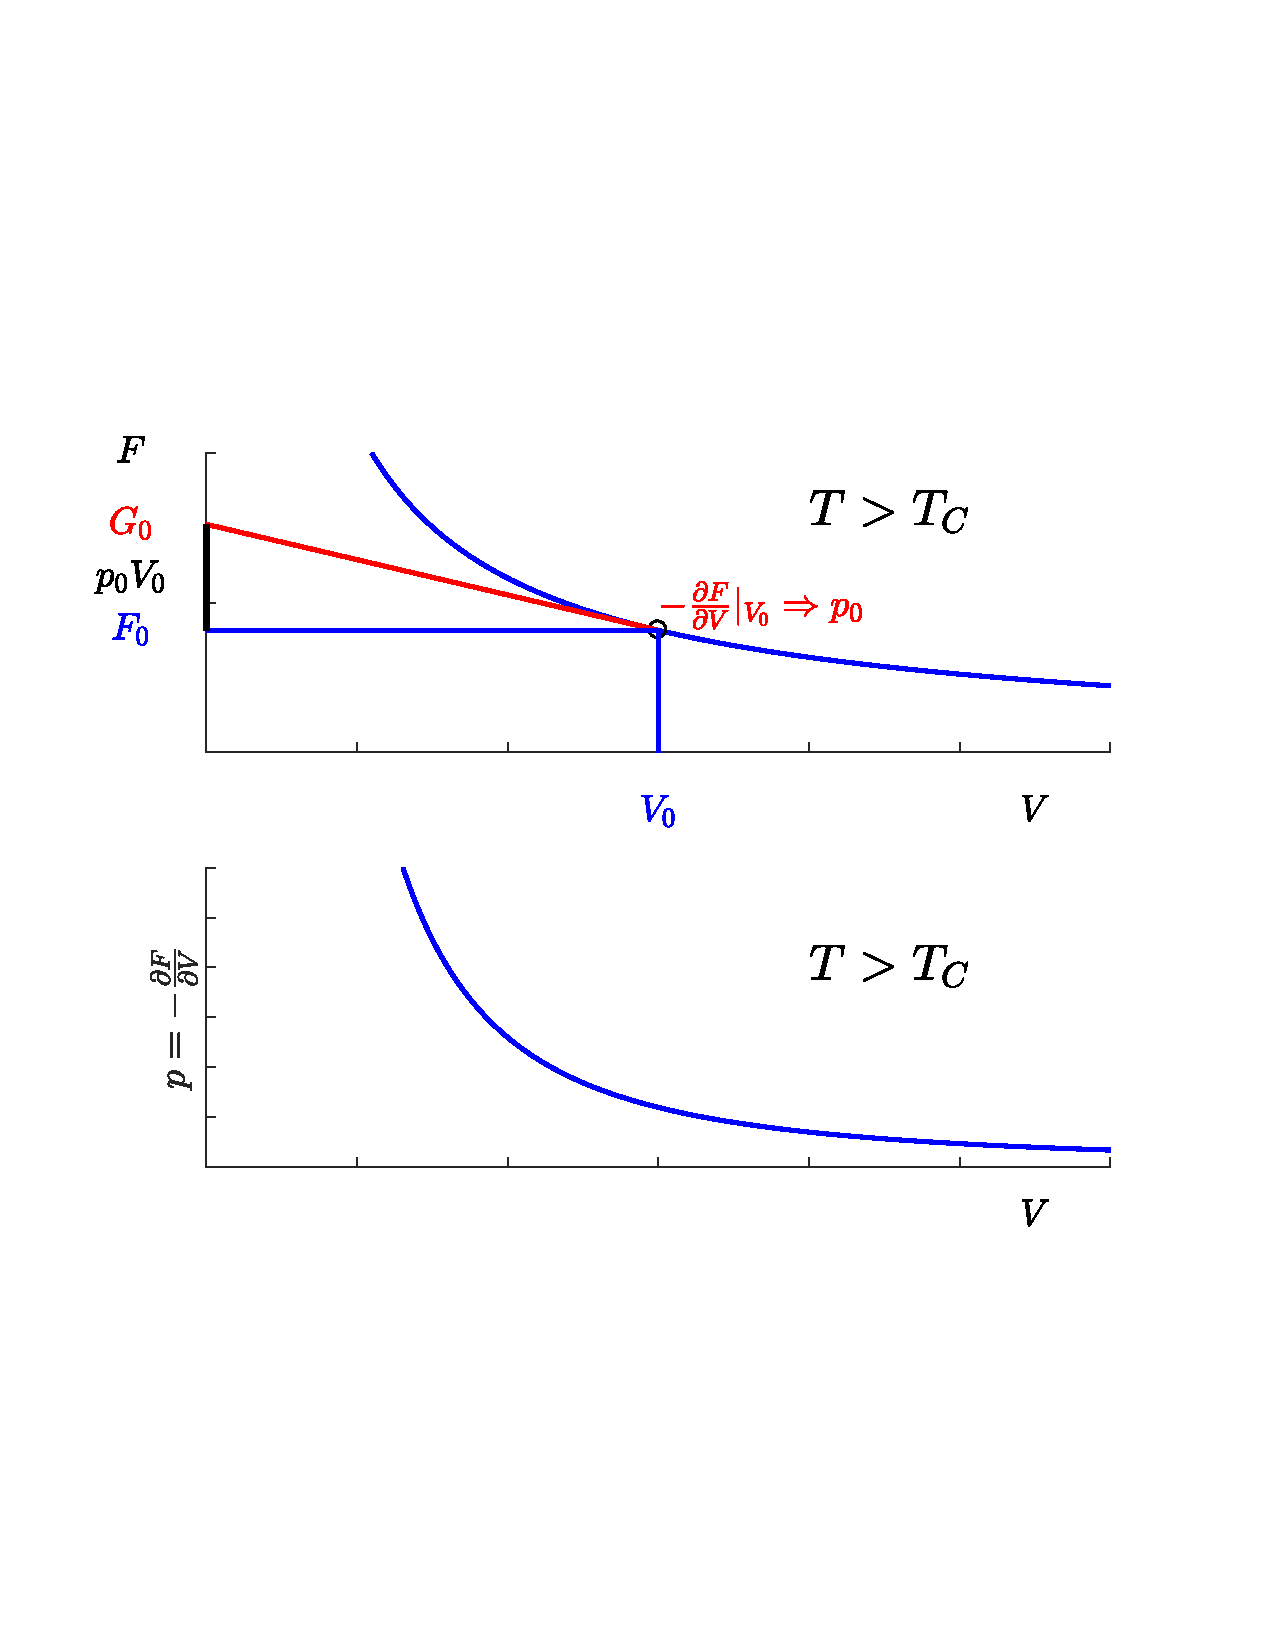
\includegraphics[width=6cm]{convex_above_Tc}
\hfill
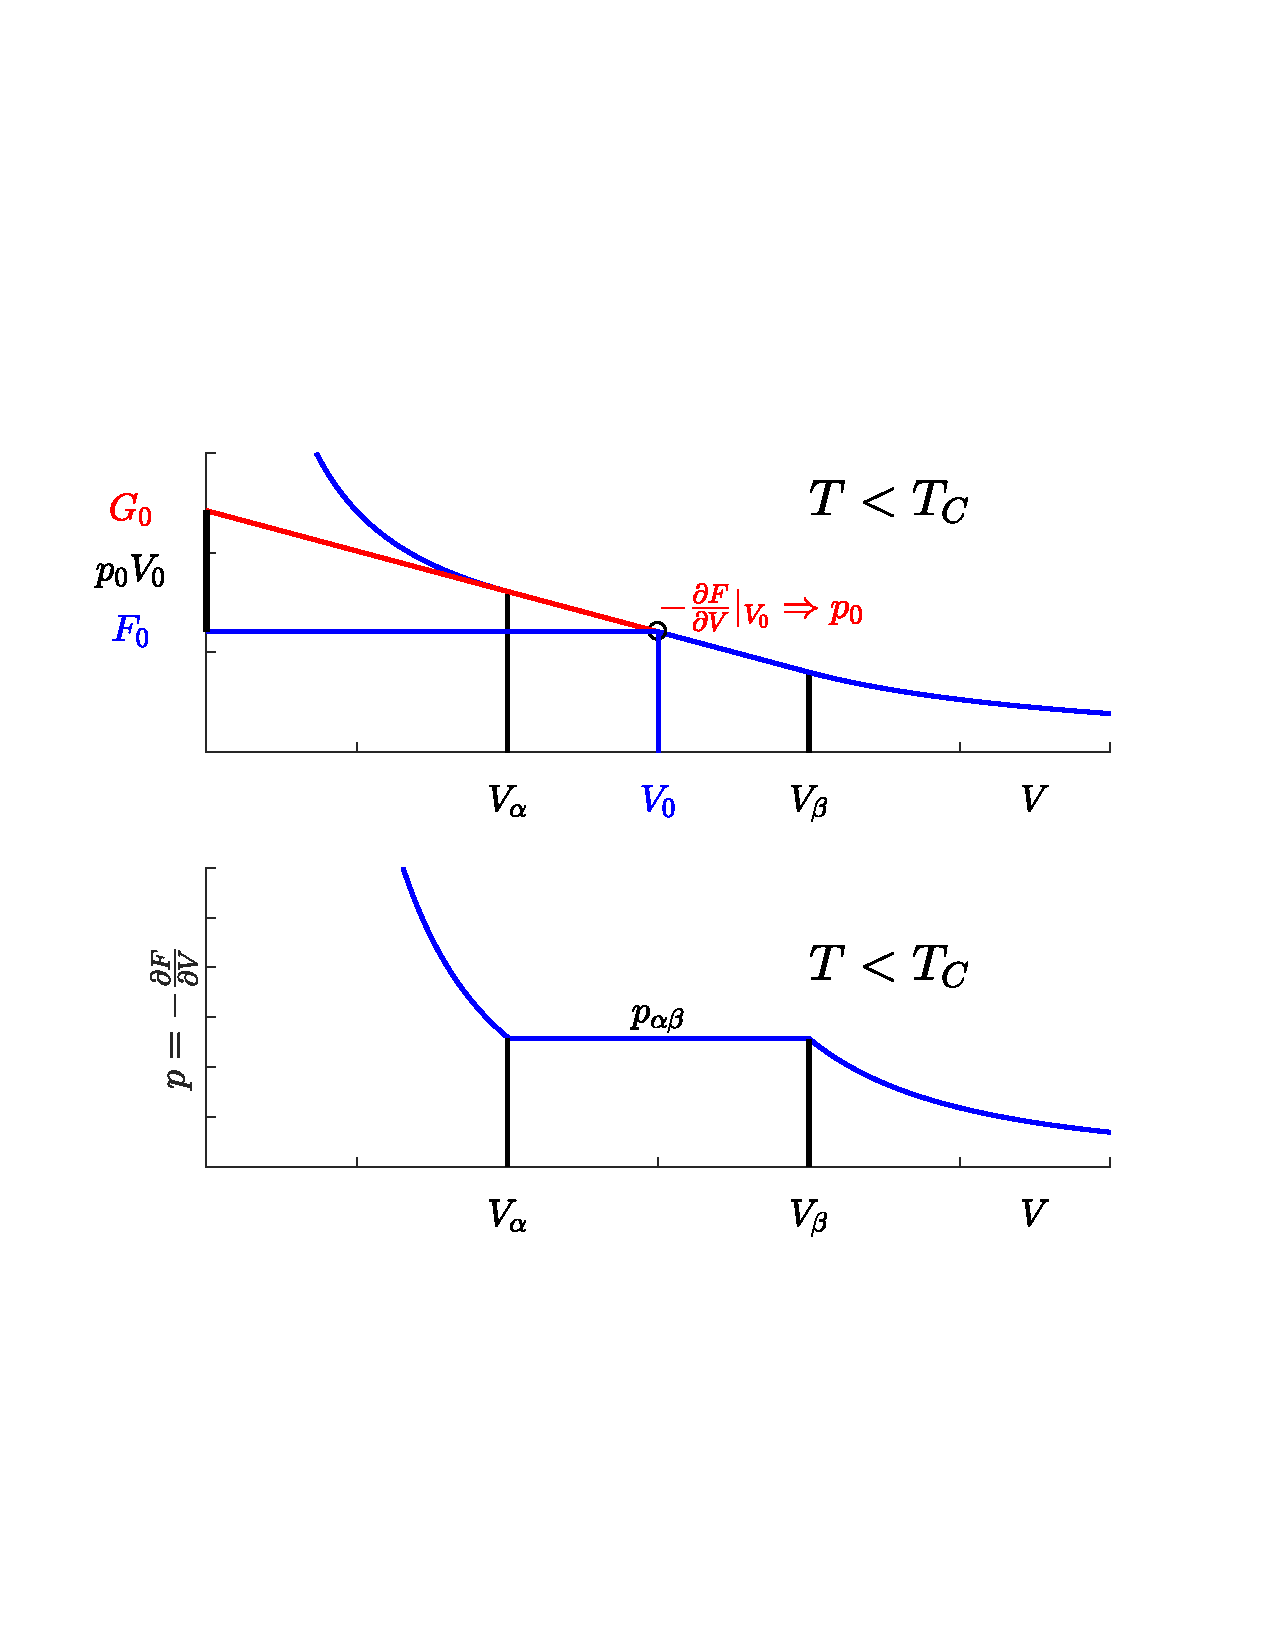
\includegraphics[width=6cm]{convex_below_Tc}
\caption{{\bf Schematic plot of free energy for $T>T_{C}$ (left) and $T<T_{C}$ (right).}}
\end{center}
\end{figure}


%\begin{figure}[ht]
%\begin{center}
%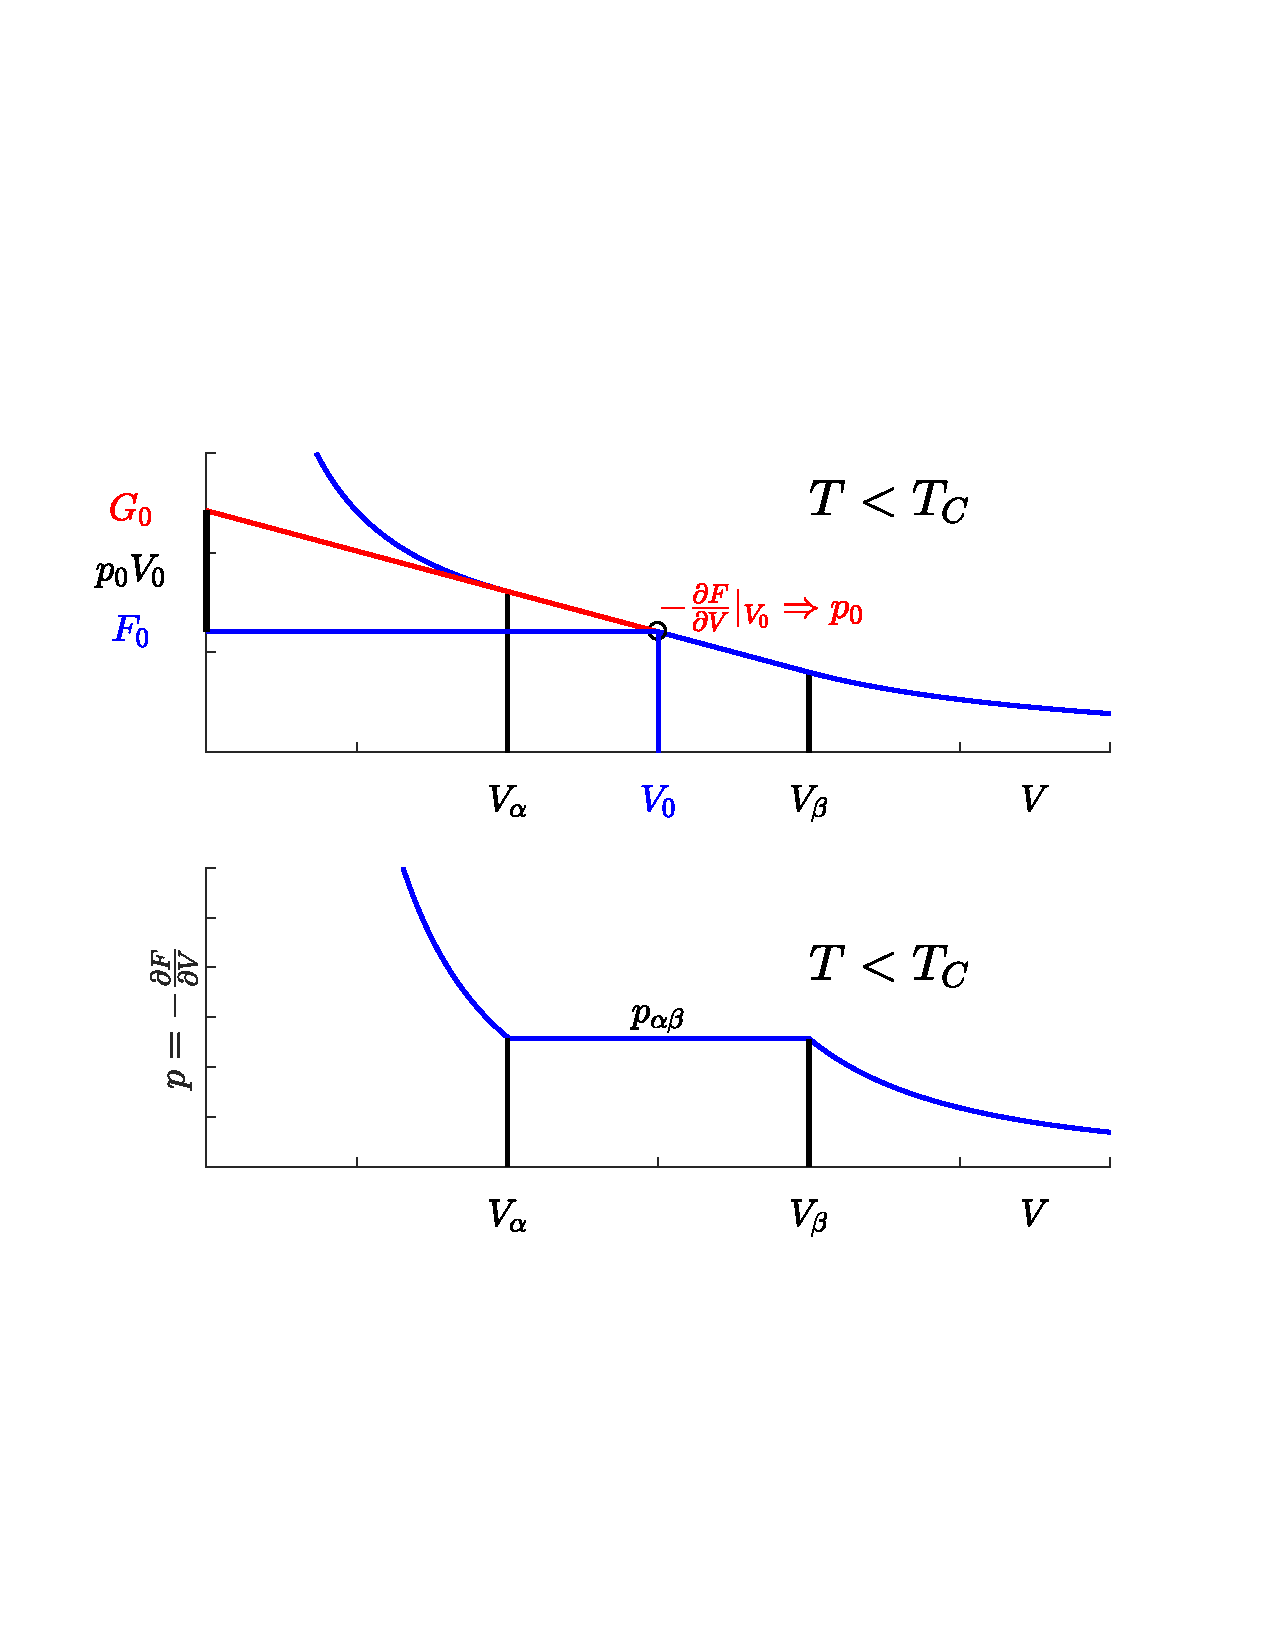
\includegraphics[width=5cm]{convex_below_Tc}
%\caption{{\bf Schematic plot of free energy for $T<T_{c}$.}}
%%\label{}
%\end{center}
%\end{figure}
%

\newpage

\subsection{$F$ and $G$ as function of $T$}

As function of temperature, both $F$ and $G$ behave similarly, since
%
\begin{align*}
-S&=\frac{\partial G}{\partial T}\at_{p}=\frac{\partial F}{\partial T}\at_{V}\;.
\end{align*}
%
At a first order phase transition the entropy $S$ shows a finite jump at $T_{c}$,
which is then associated with 
\tboxit{latent heat}{
%
\begin{align}\label{eq:}
\Delta Q &= T_{\alpha\beta} \Delta S\;.
\end{align}
%
}

$\Delta Q$ is, however not a material constant, it also depends on the state variables e.g.
for the liquid-gas system, $\Delta Q$ depends on pressure. On approaching the \blue{critical point},
$\Delta Q$ vanishes. Therefore, the definition of the order of the phase transition has to refined
\subsection{Ehrenfest classification\label{sec:ehrenfest:classification}}
\tboxit{N-th order phase transition}{
%
\begin{subequations}\label{eq:}
\begin{align}
\frac{\partial^{m} G_{\alpha}}{\partial T^{m}}\at_{p} &=
\frac{\partial^{m} G_{\beta}}{\partial T^{m}}\at_{p}
&&\forall m=1,\ldots n-1\;,\\
\frac{\partial^{m} G_{\alpha}}{\partial p^{m}}\at_{T} &=\frac{\partial^{m}  G_{\beta}}{\partial p^{m}}\at_{T}
&&\forall m=1,\ldots n-1\;.
\intertext{But}
\frac{\partial^{n} G_{\alpha}}{\partial T^{n}}\at_{p} &\ne 
\frac{\partial^{n} G_{\beta}}{\partial T^{n}}\at_{p}\\
\frac{\partial^{n} G_{\alpha}}{\partial p^{n}}\at_{T} &\ne \frac{\partial^{n} G_{\beta}}{\partial p^{n}}\at_{T}\;.
\end{align}
\end{subequations}
}
Of practical importance are first and second order phase transitions. First order phase transitions 
have already been discussed in detail. In the case of a second order phase transition,
we have
\tboxit{Second order phase transition}{
\begin{subequations}\label{eq:}
\begin{align}
G(T,p) &&\text{continuous}\\ 
\frac{\partial G}{\partial T}\at_{p},\frac{\partial G}{\partial p}\at_{T},(\text{i.e. }  
S(T,p), V(T,p)) &&\text{continuous}\\
C_{p}= -T\frac{\partial^{2} G}{\partial T^{2}}\at_{p}\;\quad 
\kappa_{T}= -\frac{1}{V}\frac{\partial^{2} G}{\partial p^{2}}\at_{T}\;\quad
&&\text{discontinous}
\end{align}
\end{subequations}
}

\section{Critical exponents\label{sec:critical:exponents}}
\blue{Second order phase transitions} are of particular interest, as they exhibit universal behaviour close 
to the phase transition. Completely different systems with second order phase transition
show a very similar power law behaviour, which shall be discussed in this section. 
We define 
%
\begin{align*}
\varepsilon &=\frac{T-T_{C}}{T_{C}}\;.
\end{align*}
%
Very often it is observed that in a close vicinity of $T_{c}$, typically
$\abs{\varepsilon} < 10^{-2}$,
%
physical observables $f(T)$ show the following behaviour
%
\begin{align*}
f(\varepsilon) &= a \varepsilon^{\varphi} \big( 1 +  b \varepsilon^{\psi} +\ldots\big)\;\psi>0\;,
\end{align*}
%
here $\varphi$ and $\psi$ are real valued exponents. This behaviour is abbreviated as
%
\begin{align}
f(\varepsilon) &\simeq \varepsilon^{\varphi}\;,
\end{align}
%
One says: $f$ behaves like $\varepsilon^{\varphi}$ and $\varphi$ is called the {\em critical exponent}.
The critical exponent is more generally defined by
%
\begin{align}\label{def:critical:exponent}
\varphi &= \lim_{\varepsilon\to 0} \frac{
\ln \abs{f(\varepsilon)} }{\ln \abs{\varepsilon}}
\end{align}
%
In general, the critical exponent depends on whether we compute it below or above $T_{c}$.
For the \blue{order parameter} it actually makes only sense below  $T_{c}$, as the order parameter
by definition is zero above $T_{c}$.

Of course, different observables may have different critical exponents. The critical exponent for 
one observable, however, is almost universal, it only depends on
\begin{itemize}
	\item spatial dimension
	\item range of the interaction
	\item spin dimensionality.
\end{itemize}

This is the so-called {\em universality hypothesis} of Griffiths.
Te range of the particle interaction is grouped into three classes:
\begin{itemize}
	\item short-range, if the interaction decreases like
%
\begin{align*}
r^{-(d+2+\alpha)}\;;\quad \alpha > 0\;.
\end{align*}
%
Where the details of the interaction are unimportant.
One finds a really universal behaviour.
\item  long-range, if  
%
\begin{align*}
r^{-(d+2+\alpha)}\;;\quad \alpha< \frac{d}{2}-2\quad\text{(always negative)}.
\end{align*}
%  
In this case, the {\em classical theories} apply (Landau Theory, van der Waals model, Weißferromagnet). In this case, however, the critical exponents are independent of the spatial dimension. 
 \item Intermediate range, if 
 %
\begin{align*}
r^{-(d+2+\alpha)}\;;\quad \frac{d}{2}-2 < \alpha < 0\;.
\end{align*}
%
The critical exponents depend on $\alpha$
\end{itemize}


Magnetic systems are typically discussed as interacting spin-systems. As spin-dimension ($n$) we understand the relevant components of the spin vector. Ising model /Potts model has $n=1$ and is considered as one-dimensional vector, the $x-y$-model has $n=2$ and the vectors are two-dimensional, and finally the Heisenberg model $n=3$ is three-dimensional. The critical exponents.



Possible behaviour:

\begin{itemize}
	\item\blue{Power law decay:} $f(\varepsilon)\simeq \varepsilon^{\varphi}$ with $\varphi >0$
	\item\blue{Power law divergence:} $f(\varepsilon)\simeq \varepsilon^{\varphi}$ with $\varphi <0$ 
	\item\blue{logarithmic divergence:} $f(\varepsilon) = a + b\ln(|\varepsilon|)$ we obtain by
	the definition of the critical exponent in \eq{def:critical:exponent} $\varphi =0$ 
\end{itemize}
In general, the critical exponent for $\varepsilon>0$ (denoted by $\varphi_{}$) can differ from that for $\varepsilon<0$ (denoted by $\varphi'$)

\subsection{Important critical exponents}


\begin{figure}[htbp]
\begin{center}
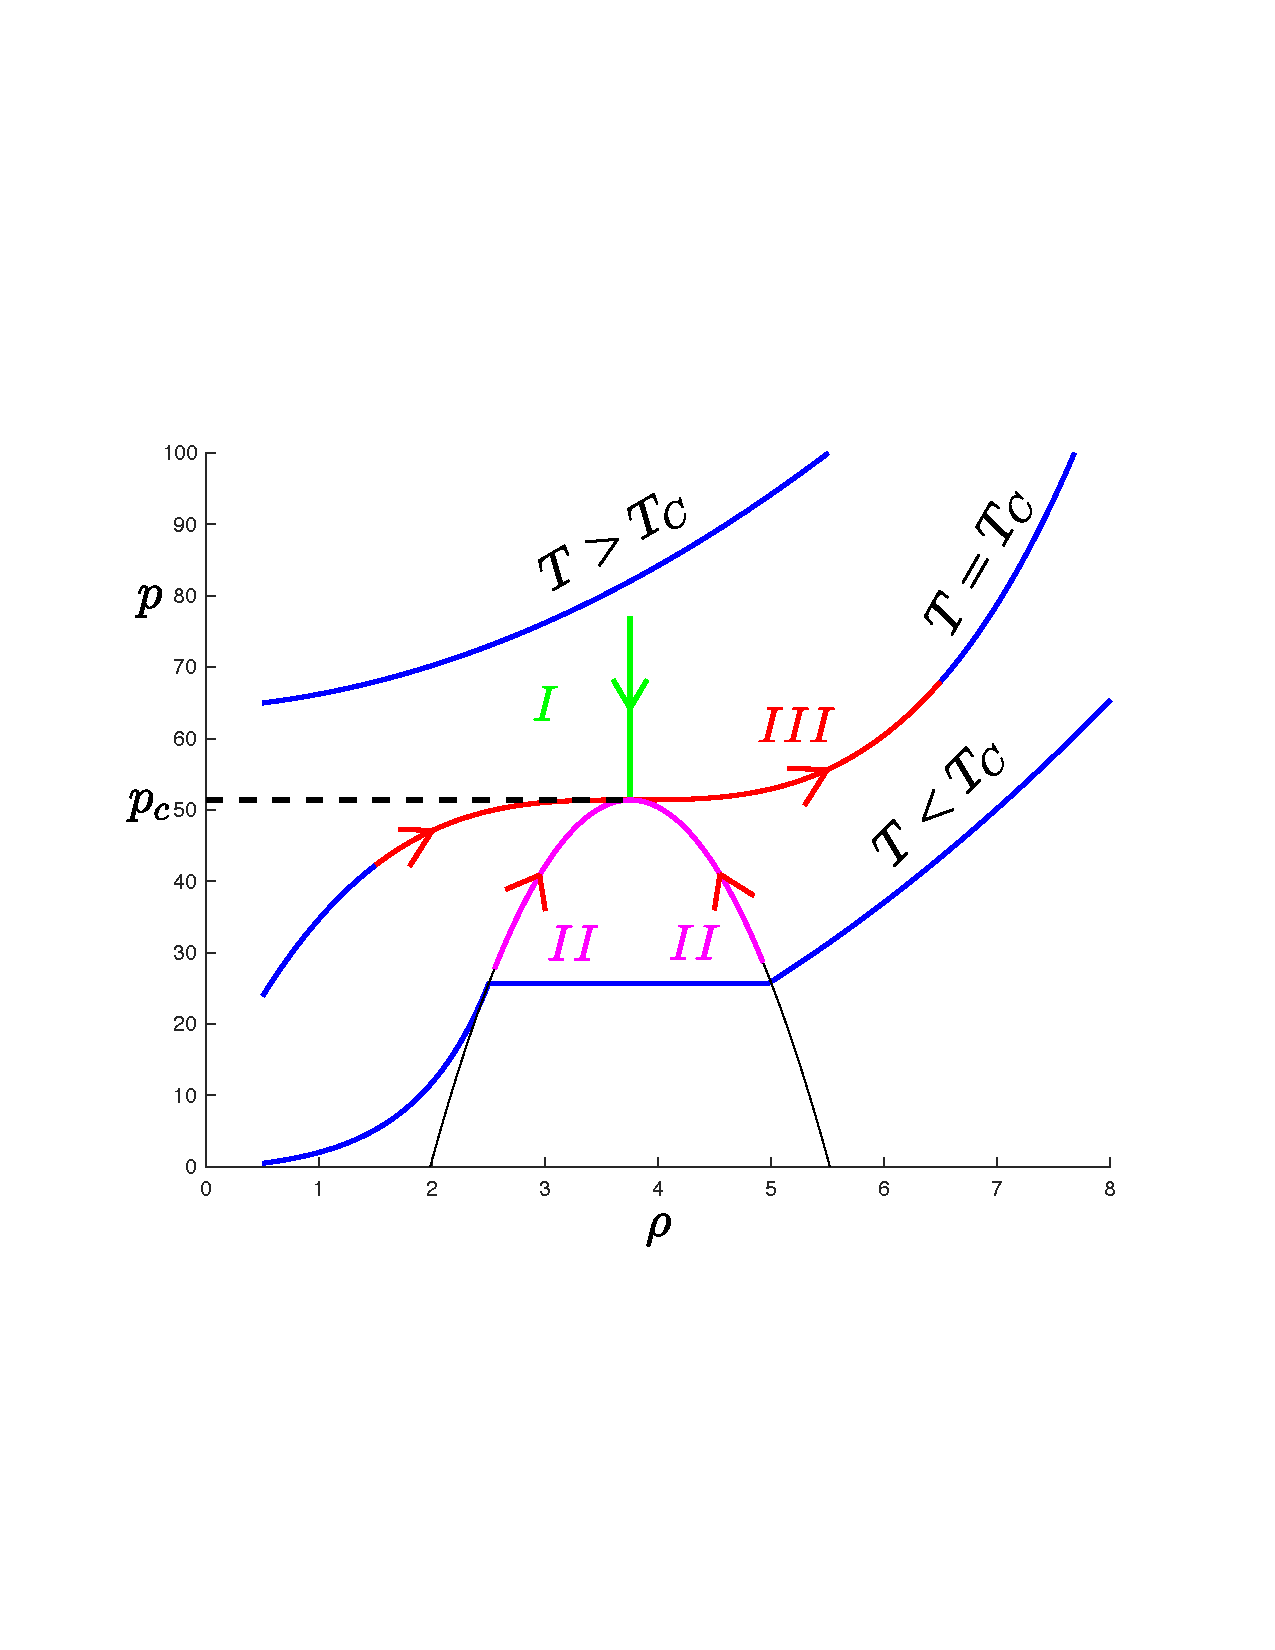
\includegraphics[width=10cm]{paths4pt}
\caption{{\bf Pressure versus density. Paths for the definition of the critical exponents.}}
%\label{}
\end{center}
\end{figure}



\begin{enumerate}
	\item Heat capacity ($\alpha:_{\pm}$) for real gases 
%
\begin{align}\label{eq:heat:capacity}
C_{V}&\simeq A_{\pm} \abs{\varepsilon}^{-\alpha_{\pm}}
:\qquad\begin{cases}
- &\text{for path II, i.e. } T \nearrow 	T_{c}, \text{with } \rho=\rho_{g,fl}\\
+ &\text{for path I, i.e. } T \searrow 	T_{c}, \text{with } \rho=\rho_{c}
\end{cases}\;.
\end{align}
%
Heat capacity ($\alpha',\alpha$) for magnets
\begin{align}\label{eq:}
C_{B}&\simeq  A_{\pm} \abs{\varepsilon}^{-\alpha_{\pm}}
:\qquad \begin{cases}
- & T \nearrow 	T_{c}, \text{with } B=0\\
 + &\text{for path I, i.e. } T \searrow 	T_{c}, \text{with } B=0
\end{cases}\;.
\end{align}
The experiment yields $\alpha_{\pm}\approx 0$. Ising 2D, exact solution, logarithmic divergence, i.e. $\alpha_{\pm}=0$. 
{\color{blue}(see section \ref{sec:Ising:2D:spec:heat}).}
Classic theories (i.e. Weißferrro-magnet, vdW gas) yield discontinuity,
which is equivalent to $\alpha_{\pm}=0$.
\item Order parameter ($\beta$ [not inverse temperature!]). A variable that exists only below $T_{c}$ and which characterises the order of the system.
E.g. magnetization $M$ or the for real gases the density difference 
$\Delta \rho = \rho_{fl}-\rho_{g}$, or rather $\Delta \rho = \rho_{fl,g}-\rho_{c}$, in the 
two-phase region
%
%
\begin{align}\label{eq:}
\frac{\Delta \rho(T)}{2 \rho_{c}} \simeq B|\varepsilon|^{\beta}&\;,\text{along path II}\\
\frac{M(T)}{M(0)} \simeq B|\varepsilon|^{\beta}&\;,\text{for zero magnetic field} \;.
\end{align}
%
The normalizations are introduced to make sure that $B$ is $O(1)$.
In principle, $\beta$ should be $\beta'$, as we are below $T_{c}$, but since the order parameter 
is only defined below $T_{c}$, it is common to use $\beta$. Typical experimental values are $0.35\pm 0.02$. classical theories yield $\beta=1/2$. 2D Ising exact, $\beta=1/8$. {\color{blue}(See section \ref{sec:Ising:2D:beta}).}
For the 3D Ising model one finds $\beta=0.325\pm 0.001$. While 3D Heisenberg gives $\beta=0.3445\pm 0.002$.

\item Compressibilities and susceptibilities ($\gamma_{\pm}$)


%
\begin{align*}
\kappa_{T} &= -\frac{1}{V}\pder{V}{p}{T} = \frac{1}{\rho} \pder{\rho}{p}{T}\;,\\
\chi_{T} &= \pder{M}{B}{T}
\end{align*}
%
\begin{align}\label{eq:}
\frac{\kappa_{T}}{\kappa^{0}_{T_{c}}}&\simeq C_{\pm} \abs{\varepsilon}^{\gamma_{\pm}}
:\qquad \begin{cases}
- &\text{for path II, i.e. } T \nearrow 	T_{c}, \text{with } \rho=\rho_{g,fl}\\
 + &\text{for path I, i.e. } T \searrow 	T_{c}, \text{with } \rho=\rho_{c}
\end{cases}\;.
\end{align}
%
Here $\kappa^{0}_{c}$ is the compressibility of the ideal gas at $T=T_{c}$, which follows (due to $\rho=\frac{p}{k_{B}T}$) from
%
\begin{align*}
\kappa &= \frac{1}{\rho} \frac{1}{k_{B}T} = \frac{1}{p}\;.
\end{align*}
%
Similarly, one uses for the normalization in the magnetic case, the result of an ideal paramagnet
%
\begin{align*}
M &=\frac{C^{*}}{T}\;,
\end{align*}
%
with $C^{*}$ being the Curie constant.
\begin{align}\label{eq:}
\frac{\chi_{T}}{\chi^{0}_{T_{c}}}&\simeq C_{\pm} \abs{\varepsilon}^{-\gamma_{\pm}}
:\qquad \begin{cases}
-&\text{for path II, i.e. } T \nearrow 	T_{c}, \text{with } H=0\\
 +&\text{for path I, i.e. } T \searrow 	T_{c}, \text{with } H=0
\end{cases}\;.
\end{align}
%
Typical experimental values differ somewhat about $\gamma\approx \gamma' \approx 1.3$.
Model calculations all yield $\gamma=\gamma'$. Classical models $\gamma=1$, 2D Ising exact,
$\gamma =7/4$, 3D Ising $\gamma\approx 1.24$, 3d Heisenberg $\gamma=1.39$.

\item Critical isotherm ($\delta$)
We define the critical pressure of the ideal gase as the pressure of the ideal gas at $T_{c}$ and 
$\rho_{c}$ via the ideal gas law
%
\begin{align*}
p_{c}^{(0)}&= k_{B}T_{c} \rho_{c}
\end{align*}
%
which clearly differs from the relation of the vdW model (see \eq{eq:p:cr}).
For the real gas we define the isothermal critical exponent as
%
\begin{align}
\frac{p-p_{c}}{p_{c}^{0}} & \simeq D \bigg| \frac{\rho-\rho_{c}}{\rho_{c}}\bigg|^{\delta} \text{sign} (\rho-\rho_{c})\;;\quad \big(\text{along the path III, } T=T_{c}  \big)\;.
\end{align}
%
If we define 
%
\begin{align*}
B_{C}^{(0)} &= \frac{k_{B} T_{c}}{\mu_{0} m}\;m
\end{align*}
%
with $m$ being the magnetic moment  per particle, then the corresponding relation for magnets reads
%
\begin{align*}
\frac{B}{B_{C}^{(0)}} &\simeq D \bigg|
\frac{M(T=T_{c},B)}{M(T=0,B=0)}
\bigg|^{\delta} \;\text{sign} (M)\;.
\end{align*}
%
Experimental values are in the range $\delta\in (4,5)$. The 2D Ising model yields $\delta=15$, which 
far off. The 3D Ising and Heisenberg model yields $\delta=4.9$ (much better). Classical theories 
yield $\delta=3$.

\item Correlation lengths ($\nu,\nu',\eta$)


We define a pair-correlation function, e.g. density-density or spn-spin,
%
\begin{align}
g(\vv r,\vv r') &= \avg{\Delta \rho(\vv r) \Delta \rho(\vv r')}\\
g_{ij} &= \avg{\Delta \vv S_{i} \Delta \vv S_{j}}\;.
\end{align}
%
In the critical regions they behave approximately like
%
\tboxit{Ornstein-Zernike function}{
\begin{align}\label{eq:Ornstein:Zernike}
g(\vv r,\vv r') &=c_{0}\;\frac{e^{-\frac{|\vv r - \vv r'|}{\xi(T)}}}{\abs{\vv r-\vv r'}}\\
g_{ij} &= g(\vv r_{i},\vv r_{j}) \;,
\end{align}}
%
with $\xi(T)$ is the correlation length.
It diverges on approaching the critical point.
For real gases one defines
%
\begin{align}\label{eq:}
\xi\simeq D_{\pm} \abs{\varepsilon}^{-\nu_{\pm}}
:\qquad \begin{cases}
-&\text{on path II}\;,\\
+&\text{on path I}\;.
\end{cases}
\end{align}
%
For magnets
\begin{align}\label{eq:}
\xi\simeq D_{\pm} \abs{\varepsilon}^{-\nu_{\pm}}
:\qquad
\begin{cases}
-	&\text{for }	T\nearrow T>T_{C}, B=0	\;,\\
+			&\text{for }	T\searrow T>T_{C}, B=0	\;.
\end{cases}
\end{align}
%
%
Finally, we also introduce the  pair-correlation function at the critical temperature $T=T_{c}$. According to the Ornstein-Zernike formula
in \eq{eq:Ornstein:Zernike}, at $T=T_{c}$ the correlation length is infinite and, therefore, the pair-correlation would decrease like
$1/\abs{\vv r-\vv r'}$. This is, however, not the case for real systems.
The behaviour is slightly different and expressed by
%
\begin{align*}
g(\vv r,\vv r') &=\big|\vv r-\vv r'\big|^{-(d-2+\eta)}
\begin{cases}
p=p_{C}  &\text{, real gases}\;,\\
B=0\text{, magnets}\;.
\end{cases}
\end{align*}
%
The Ornstein-Zernike formula would imply $\eta = 3-d$. For the other critical exponents $\nu,\nu'$ the deviation  from the $1/r$ dependence is negligible, as the the correlation length is obtained
from the slope of a fit of 
%
\begin{align*}
\ln(g(r)) &= c_{0} -\frac{r}{\xi(T)} - (d-2+\eta)\ln(r)
\end{align*}
%
versus $r$. Here the last term enters only logarithmically in $r$.




\end{enumerate}


\subsection{Scaling laws}
\blue{Generalized homogeneous functions} $f(x,y,\ldots)$ in several variables have the 
following property for arbitrary real $\lambda$
%
\begin{align}\label{eq:}
f(\lambda^{a_{x}} x,\lambda^{a_{y}}y,\ldots ) &=\lambda f(x,y,\ldots)\;,
\end{align}
%
where $a_{x},a_{y},\ldots$ can be any real numbers. An example would be
%
\begin{align*}
f(x,y) &= 4 x^{3} + 7 y^{8}\;,
\end{align*}
%
with $a_{x}=1/3$ and $a_{y}=1/8$, while 
%
\begin{align*}
f(x,y) &= x + 6 x^{2} + xy + y^{5}
\end{align*}
%
is no generalized homogeneous function. Next we will define the
{\color{blue}scaling hypothesis} in the case of the free energy $F(T,B)$ of a magnetic system. We are only interested in the non-analytic parts of $F$
near $T_{C}$ which we denote by
$F(\varepsilon,B) $.

\tboxit{Scaling hypothesis}{
%
\begin{align}\label{eq:}
F(\lambda^{a_{\varepsilon}}\varepsilon,\lambda^{a_{B}}B) &=
\lambda \;F(\varepsilon,B)\;.
\end{align}
%
}
This is not yet strictly proven in general, but there are many important
cases where the scaling hypothesis is fulfilled.

Now we can use the scaling hypothesis to express the critical exponents
in terms of the scaling parameters $a_{\varepsilon}$ and $a_{B}$.
Differentiation w.r.t. $B$ yields
%
\begin{align*}
 \frac{\partial }{\partial b}
 F(\lambda^{a_{\varepsilon}}\varepsilon,b) \bigg|_{b= \lambda^{a_{B}}B}
\; \lambda^{a_{B}}
&\overset{!}{=} \lambda
\frac{\partial }{\partial B}
F(\varepsilon,B)\;.
\end{align*}
%
Now we have 
%
\begin{align*}
M &= -\frac{\partial F}{\partial B}
\end{align*}
%
and therefore  we have
%
\begin{align}
\lambda^{a_{B}} 
M(\lambda^{a_{\varepsilon}}\varepsilon,\lambda^{a_{B}}B) 
&= \lambda M(\varepsilon,B)\;.
\end{align}
%
\begin{enumerate}
	\item[a)] {\color{blue}Exponent $\beta$:} We use $B=0$ and obtain
%
\begin{align*}
\lambda M(\varepsilon,0) &=M(\lambda^{a_{\varepsilon}}\varepsilon,0) \;,
\end{align*}
%
which is valid for any $\lambda$, also for 
%
\begin{align*}
\lambda&=(-\varepsilon)^{-1/a_{\varepsilon}}\;,
\end{align*}
%
resulting in 
%
\begin{align*}
M(\varepsilon,0) &= (-\varepsilon)^{\frac{1-a_{B}}{a_{\varepsilon}}} M(-1,0)\simeq (\varepsilon)^{\frac{1-a_{B}}{a_{\varepsilon}}} \;.
\end{align*}
%
Hence, 
%
\begin{align*}
\beta=\frac{1-a_{B}}{a_{\varepsilon}} \;.
\end{align*}
%
\item[b)] {\color{blue}Exponent $\delta$ (critical isotherm):}
Next we use $\varepsilon=0$ and have
%
\begin{align*}
M(0,B) &= \lambda^{a_{B}-1}\;M(0,\lambda^{a_{B}}B)\;.
\end{align*}
%
Here we choose $\lambda =B^{-1/a_{B}}$ and obtain
%
\begin{align*}
M(0,B) &\simeq  B^{\frac{1-a_{B}}{a_{B}}}\\
B &\simeq M^{\frac{a_{B}}{1-a_{B}}}\;,
\end{align*}
%
and hence $\delta=\frac{a_{B}}{1-a_{B}}$.
In summar, we have
%
\begin{align}\label{eq:}
a_{B} &= \frac{\delta}{1+\delta}\\
a_{\varepsilon} &= \frac{1}{\beta}\frac{1}{1+\delta}\\
\end{align}
%
\end{enumerate}
We can express further critical exponents in terms of the scaling parameters, which then in turn allows to find relations among the 
critical exponents:
%
From the scaling laws one finds
\begin{align}
\alpha&=\alpha'\;;\quad
\gamma=\gamma'\;;\quad\nu=\nu'\;.
\end{align}
%
and also
%
\begin{align}
\alpha+2\beta+\gamma &=2\\
\alpha+\beta (1+\delta)&=2\\
\beta &=\frac{\gamma}{\delta-1}\\
\nu &=\frac{\gamma}{2-\eta}\;.
\end{align}
%

	   
% extra material: \subsection{Pottsmodel}
It can be considered as generalisation of the Ising model, where the spin can take on more than just two values. Usually they are enumerated $s\in \{1,2,\ldots,q\}$. It is called the {\em q-state Potts model}. The   Hamiltonian of the Potts model reads
%
\tboxitp{Pottsmodel}{$q$ states}{
\begin{align}
H_{P} &= -J \sum_{ij} \delta_{s_{i}s_{j}}\;,
\end{align}}
%
i.e. when spins on neighbouring sites are equal, they experience a lower energy ($E=-J$)
than when the have different spin values ($E=0$).
The Potts model is used to study  the behaviour of ferromagnets and other
phenomena of solid-state physics. 

Apart from statistical physics it is also used in computer science (signal processing) and biology (neural networks). 

The strength of the Potts model is not so much 
that it models these physical systems well; it is rather that the one-dimensional case is exactly 
solvable, and that it has interesting physical properties. For $d\ge 2$ it shows a phase transition.
It is second order for $q\le 4$ and first order for $q>4$.






\subsection{Maxwell Relations}

We know
%
\begin{align*}
d U(S,V,N) &= T dS -p dV +\mu dN
\end{align*}
%
Hence
%

\begin{align*}
\pder{U(S,V,N)}{S}{V,N} &= T(S,V,N)\\
\pder{U(S,V,N)}{V}{S,N} &= -p(S,V,N)\;.
\end{align*}
%
From this we obtain
%
\begin{align*}
\pder{T}{V}{S,N} &=\frac{\partial }{\partial V}\bigg(\pder{U}{S}{V,N}\bigg)\at_{S,N}
 =\frac{\partial }{\partial S}\bigg(\pder{U}{V}{S,N}\bigg)\at_{V,N}
 =-\pder{p}{S}{V,N}
\end{align*}
%
In the following we use the convention
%
\begin{align*}
\frac{\partial^{2}f(x,y,z)}{\partial x\partial y } 
=\frac{\partial }{\partial y}\bigg(\pder{f}{x}{y,z}\bigg)\at_{x,z}\;.
\end{align*}
%
and we can simplify the former equation to
%
\begin{align*}
\pder{T}{V}{S,N} &= -\pder{p}{S}{V,N}
 =\frac{\partial^{2}U(S,V,N) }{\partial S\partial V}\;.
\end{align*}
%
Similarly we find with
\begin{align*}
\pder{F(T,V,N)}{T}{V,N} &= -S(T,V ,N)\\
\pder{F(T,V,N)}{V}{S,N} &= -p(T,V ,N)\;.
\end{align*}
%
the relation
%
\begin{align*}
\pder{S(T,V,N)}{V}{T,N} & =\pder{p(T,V,N)}{T}{V,N}
=-\frac{\partial^{2} F(T,V,N)}{\partial V\partial T}
\end{align*}
%
Based on the free enthalpy $G(T,p,N)$
we obtain with
%
\begin{align*}
\pder{G(T,p,N)}{T}{p,N} &= -S(T,p ,N)\\
\pder{G(T,p,N)}{p}{S,N} &= V(T,p ,N)\;.
\end{align*}
%
the relation
%
\begin{align*}
-\pder{S(T,p,N)}{p}{T,N} & =\pder{V(T,p,N)}{T}{p,N}
=\frac{\partial^{2} G(T,p,N)}{\partial p\partial T}
\end{align*}
%
Finally, we introduce the {\em enthalpy} $H(S,p,N)$ via the Legendre transformation of
$U(S,V,N)$ with respect to $V$, i.e.
%
\begin{align*}
H(S,p,N) &= U(S,V,N) + pV\;,
\end{align*}
% 
for which we have
%
\begin{align*}
\pder{H(S,p,N)}{S}{p,N} &= T(S,p ,N)\\
\pder{H(S,p,N)}{p}{S,N} &= V(S,p ,N)\;.
\end{align*}
%
Then we find
\begin{align*}
\pder{T(S,p,N)}{p}{S,N} & =\pder{V(S,p,N)}{S}{p,N}
=\frac{\partial^{2} H(S,p,N)}{\partial p\partial S}
\end{align*}

We summaries these results 
\tboxit{Maxwellrelations}{
\begin{subequations}\label{eq:}
\begin{align}
\pder{T(S,V,N)}{V}{S,N} &= -\pder{p(S,V,N)	}{S}{V,N}
 &&=\frac{\partial^{2}U(S,V,N) }{\partial S\partial V}\\
\pder{S(T,V,N)}{V}{T,N} & =\pder{p(T,V,N)}{T}{V,N}
&&=-\frac{\partial^{2} F(T,V,N)}{\partial V\partial T}\\
-\pder{S(T,p,N)}{p}{T,N} & =\pder{V(T,p,N)}{T}{p,N}
&&=\frac{\partial^{2} G(T,p,N)}{\partial p\partial T}\\
\pder{T(S,p,N)}{p}{S,N} & =\pder{V(S,p,N)}{S}{p,N}
&&=\frac{\partial^{2} H(S,p,N)}{\partial p\partial S}\;.
\end{align}
\end{subequations}
}

\subsection{Ehrenfest equations}

Next we derive the analogue of Clausius-Clapeyron for second order phase transitions.
In this case, $S$ and $V$ are continuous when crossing 
the phase boundary. Along a phase boundary between phase $\alpha$ and $\beta$ we therefore have in the Gibbs ensemble $(T,p,N)$ fixed
%
\begin{align*}
S_{\alpha}(T,p,N) &= S_{\beta}(T,p,N)\\
V_{\alpha}(T,p,N) &= V_{\beta}(T,p,N)\;,
\end{align*}
%
and also
%
\begin{align*}
dS_{\alpha} &= dS_{\beta}\\
dV_{\alpha} &= dV_{\beta}\;.
\end{align*}
%
We can use these equations, to obtain $dp/dT$ along the phase boundary.
We combine  these equation as
%
\begin{align*}
dX_{\alpha}(T,p,N) &= dX_{\beta}(T,p,N)\;,
\end{align*}
%
where $X$ stands either for $S$ or $V$.
Since $N$ is fixed, it will not vary along the phase boundary. We therefore have
\begin{align*}
\pder{X_{\alpha}}{T}{p,N} dT +\pder{X_{\alpha}}{p}{T,N} dp
&=\pder{X_{\beta}}{T}{p,N} dT +\pder{X_{\beta}}{p}{T,N} dp\;,
\end{align*}
%
from which we obtain
%
\begin{align*}
\bigg(\pder{X_{\beta}}{T}{p,N}-\pder{X_{\alpha}}{T}{p,N}\bigg)dT
&=
-\bigg(\pder{X_{\beta}}{p}{T,N}-\pder{X_{\alpha}}{p}{T,N}\bigg)dp\\
\frac{dp}{dT}
&=
-\frac{\pder{X_{\beta}}{T}{p,N}-\pder{X_{\alpha}}{T}{p,N}}
{\pder{X_{\beta}}{p}{T,N}-\pder{X_{\alpha}}{p}{T,N}}
:=
-\frac{\Delta \pder{X_{\beta}}{T}{p,N}}
{\pder{\Delta X_{\beta}}{p}{T,N}}
\end{align*}
%
If we insert $S$ for $X$ we find
%
\begin{align}\label{eq:}
\frac{d p}{dT} &=-\frac{\Delta \pder{S}{T}{p,N}}
{\pder{\Delta S}{p}{T,N}}\;.
\end{align}
%
We use 
%
\begin{align*}
\pder{S}{T}{p,N} &= \frac{1}{T} C_{p}\;,
\end{align*}
%
and from the Maxwell relations we use 
%
\begin{align*}
\pder{S}{p}{T,N} &= -\pder{V}{T}{p,N} \;.
\end{align*}
%
The change in volume w.r.t. temperature is related to the 
$\alpha$
%
\tboxitp{coefficient of thermal expansion}{for constant pressure}{
\begin{align}
\alpha_{p} &:= \frac{1}{V}\pder{V}{T}{p,N}  
\end{align}}
%
With these response functions, we find
%
\begin{align}\label{eq:}
\frac{dp}{dT}\at_\text{ph.b.} &= \frac{1}{V T}\frac{\Delta C_{p}}{\Delta \alpha_{p}}\;.
\end{align}
%
Alternatively, if we use $V$ as $X$, we have
%
\begin{align}\label{eq:}
\frac{d p}{dT} &=-\frac{\Delta \pder{V}{T}{p,N}}
{\pder{\Delta V}{p}{T,N}}\;.
\end{align}
%
Here we employ the relations
%
\begin{align*}
\alpha_{p} &= \frac{1}{V} \pder{V}{T}{p,N}\\
\kappa_{p} &= -\frac{1}{V} \pder{V}{p}{T,N} \;,
\end{align*}
%
and find
\begin{align}\label{eq:}
\frac{dp}{dT}\at_\text{ph.b.} &= \frac{\Delta \alpha_{p}}{\Delta \kappa_{p}}\;.
\end{align}

In summary we have the
\tboxit{Ehrenfest equations}{
%
\begin{align}\label{eq:}
\frac{dp}{dT}\at_\text{ph.b.} &= \frac{\Delta \alpha_{p}}{\Delta \kappa_{p}}
=\frac{1}{V T}\frac{\Delta C_{p}}{\Delta \alpha_{p}}\;.
\end{align}
%
}


\section{Ising again}

%
\begin{align*}
s&:=\sinh(2K)\\
f=\frac{F}{JN} &= -K\bigg[\frac{\ln(2)}{2} +\frac{1}{4\pi}\int_{0}^{2\pi}
\log\bigg( 1+ s^{4} + \sqrt{1+s^{4} -2 s^{2}\cos(x)}\bigg) dx\bigg]
\end{align*}
%
$T_{c}$ from
%
\begin{align*}
s_{c} &= \sinh(2K_{c}) = 1\\
K_{c} &= J \beta_{c} = 0.440687\\
\frac{k_{B} T_{c}}{J} &=2.26919\;.
\end{align*}
%
%
\begin{align*}
u=\frac{U}{JN} &= -   \coth(2 K)
\bigg[ 
1+\frac{2( 2 \tanh^{2}\big( 2K \big)-1 )}{\pi}
\int_{0}^{\pi/2}\frac{1}
{
\sqrt{1-\frac{4k}{(1+k)^{2}}\sin^{2}(x)}
}
 \bigg]
\end{align*}
%


For $T\le T_{c}$
%
\begin{align*}
M(T) &= \bigg[ 1 - \bigg(\sinh^{-4}(2K)  \bigg) \bigg]^{1/8}\;.
\end{align*}
%

%
\begin{align*}
S &= -\frac{\partial F}{\partial T} = -\frac{\partial F}{\partial \beta} \frac{d\beta}{dT}
= \frac{J}{k_{B}T^{2}} \frac{\partial F}{\partial J \beta} \\
&= \frac{K}{T} \frac{\partial F}{\partial K} = \frac{K J N}{T} \frac{\partial f}{\partial K}\\
\frac{S}{N}&= k_{B}\frac{K J}{k_{B}T} \frac{\partial f}{\partial K}\\
s&=\frac{S}{k_{B}N}= K^{2} \frac{\partial f}{\partial K}\\
\end{align*}
%
%
\begin{align*}
U &= F+TS = f J N + T s k_{B} N  \\
&= JN\bigg( f  + \frac{T  k_{B}}{J} s\bigg) \\
u&= f + \frac{s}{K}
\end{align*}
%

%
\begin{align*}
s&= K f - K^{3}\frac{d}{dK} \frac{1}{4\pi}\int_{0}^{2\pi}
\log\bigg( 1+s^{2} +  \sqrt{1+s^{4} -2 s^{2}\cos(x)}\bigg) dx\\
&= K f - K^{3}\bigg(\frac{d}{ds} \frac{1}{4\pi}\int_{0}^{2\pi}
\log\bigg( 1+s^{2} +  \sqrt{1+s^{4} -2 s^{2}\cos(x)}\bigg) dx\bigg)
\;\frac{d}{dK} \sinh(2K)\\
&= K \bigg(f - K^{2}\bigg(\frac{d}{ds} \frac{1}{4\pi}\int_{0}^{2\pi}
\log\bigg( 1+s^{2} +  \sqrt{1+s^{4} -2 s^{2}\cos(x)}\bigg) dx\bigg)!
\;2 \sqrt{1+s^{2}}\bigg)\;.
\end{align*}
%

%
\begin{align*}
u &= f + \frac{s}{K}
\end{align*}
%




	

\chapter{Magnetism}

In this chapter we will study further theories on magnetism, including first the general Hamiltonian for a magnetic system and then looking at different approaches to obtain an expression for magnetization in different cases - some of which more involved than others.

Lastly, we will revisit collective magnetism by introducing the Heisenberg Hamiltonian as a generalization of the by now well-known Ising model.
\section{Hamiltonian}

The hamiltionian reads
%
\begin{align}\label{eq:H:a}
H = \sum_{j}\bigg( \vv p_{j} + e \vv A(\vv r_{j}) \bigg)^{2} 
+ H_\text{Coul}- \sum_{j}  m^{s}_{j}B(\vv r_{j}) +H_{rel}
\end{align}
%
So far, this  hamiltonian describes any arbitrary system, from isolated atoms up to any crystal.
The first term describes the coupling of the electrons to the electromagnetic field in combination with  the kinetic energy of the electrons, the second contains Coulomb interaction of the electrons to the atomic core and the electron-electron interaction and last term covers the interaction of the magnetic moment of the electronic spins 
to the external field. The spin of electron $j$, denoted by $\vv S_{j}$ corresponds to a magnetic moment
%
\begin{align}\label{eq:magmo:spin}
\vv m_{j}^{s} &= - \frac{g_{e} e}{2m } \vv S_{j} 
= -\frac{g_{e} \mu_{B}}{\hbar  } \vv S_{j} 
\end{align}
%
with $g_{e}=2.0023$ being the Land\'e Factor for the electron,
and the Bohr magneton
%
\begin{align}
\mu_{B} &= \frac{e \hbar}{2m}\;.
\end{align}
%
The last term in \eq{eq:H:a} covers relativistic effects, such as the spin orbit coupling, which we will briefly discuss later on.
In the hamiltonian the dipole-dipole interaction of the spins is neglected, as it is of minor importance.
First, we transform  the first part of the hamiltonian 
%
\begin{align*}
\bigg( \vv p_{j} + e \vv A(\vv r_{j}) \bigg)^{2} &= \vv p_{j}^{2} +e  \vv p_{j}  \vv A(\vv r_{j})
+e  \vv A (\vv r_{j}) \vv p_{j}  + e^{2}\vv A^{2}( \vv r_{j})
\end{align*}
%
We use the Coulomb gauge, in which
%
\begin{align*}
\text{div} \vv A(\vv r) &= 0
\end{align*}
%
holds. Moreover, we will only consider a homogeneous magnetic field
$\vv B$, for which in the Coulomb gauge we can write
%
\begin{align*}
\vv A(\vv r) &= \frac{1}{2}\vv B\times \vv r\;.
\end{align*}
%
In this case 
%
\begin{align*}
\vv p_{j} \vv A(\vv r_{j}) &= 
\frac{1}{2}\vv p_{j} \cdot \big(\vv B\times \vv r_{j}\big)\;.
\end{align*}
%
We have to take into account that $\vv P$ and $\vv r$ are operators, while 
$\vv B$ is a classical vector. Then the spin-term simplifies to
%
\begin{align*}
\sum_{j}  m^{s}_{j}B(\vv r_{j}) &= \vv B \;\sum_{j} m^{s}_{j}\;.
\end{align*}
%
Moreover, we need
%
\begin{align*}
\vv p\cdot \big( \vv B\times \vv r \big) 
&=p_{i} \varepsilon_{ijk} B_{j} r_{k}\\
&=-B_{j}  \varepsilon_{jik} p_{i} r_{k}\\
&=B_{j}  \varepsilon_{jki} r_{k} p_{i} \;.
\end{align*}
%
In the last step we have used that $r_{k}$ and $p_{j}$ commute for different indices. If the indices of $r$ and $p$ would be equal, then the Levi-Civita symbol would vanish.
Hence,
%
\begin{align}\label{eq:}
\vv p_{j}\cdot \big( \vv B\times \vv r_{j} \big)  &=
\vv B\cdot \big( \vv r_{j}\times \vv p_{j}\big) =\vv B \cdot \vv L_{j}\;.
\end{align}
%
Similarly, we find
\begin{align*}
\big( \vv B\times \vv r \big) \cdot \vv p
&= \varepsilon_{ijk} B_{j} r_{k}p_{i}\\
&=B_{j}  \varepsilon_{jki} r_{k} p_{i} \;.
\end{align*}

We still need 
%
\begin{align*}
\vv A^{2}(r) &= \frac{1}{4} \bigg( \vv B \times \vv r \bigg)^{2}\\
&=\frac{1}{4}\varepsilon_{ijk}\varepsilon_{imn} B_{i} r_{j} 
B_{m}r_{n}\\
&=\frac{1}{4}\bigg(B_{i} r_{j} B_{i}r_{j}
-B_{i} r_{i} B_{j}r_{j}\bigg)\\
&=\frac{1}{4}\big(\vv B^{2}\vv r^{2} -(\vv B\cdot \vv r)^{2}\big)\;.
\end{align*}
%

In total we therefore find
%
\begin{align*}
H
&=\frac{1}{2m}\sum_{j}\vv p_{j}^{2} 
+\frac{e}{2m}\vv B \sum_{j}\cdot \vv L_{j} 
+\frac{e^{2}B^{2}}{8m}\sum_{j}\big(\vv B^{2}\vv r_{j}^{2}-(\vv B\cdot \vv r_{j})^{2}\big)
+ H_\text{Coul}
- \vv m^{s} \cdot \vv B\;,
\end{align*}
%
where $\vv m^{s}$ is the total magnetic moment of all spins. We also relate the angular momentum with the magnetic moment
%
\begin{align*}
\vv m^{L}_{j} &= - \frac{e}{2m} \vv L_{j}= - \frac{\mu_{B}}{\hbar} \vv L_{j}\\
\vv m^{L} &= - \frac{e}{2m} \sum_{j}\vv L_{j}= - \frac{\mu_{B}}{\hbar} \sum_{j}\vv L_{j}\;.
\end{align*}
%
Then the hamiltonian simplifies to 
\begin{align*}
H
&=\frac{1}{2m}\sum_{j}\vv p_{j}^{2} 
+ H_{dia}
+ H_\text{Coul}
- \vv m^{perm} \cdot \vv B\;,\\
H_{dia} &=
\frac{e^{2}B^{2}}{8m}\sum_{j}\big(\vv B^{2}\vv r_{j}^{2}-(\vv B\cdot \vv r_{j})^{2}\big)\;,
\end{align*}
with the total {\color{blue}\em permanent} magnetic moment defined by
%
\begin{align}
\vv m^{perm} &= \vv m^{s} + \vv m^{L}= -\frac{\mu_{B}}{\hbar}\big( \vv L + g_{e}\vv S \big)\;.
\end{align}
%
It results in {\color{blue}\em paramagnetism}.

The permanent moments tend to align in the magnetic field, while thermal fluctuations have  the opposite effect.
There is yet another  term in the hamiltonian \eq{eq:H:a} that contains magnetic moments resulting from the electronic motion: the diamagnetic term  $H_{dia}$.
One can show that the total magnetic moment, defined as
\begin{align*}
\vv m &= \vv m^{perm} + \vv m^{ind}\;,
\end{align*}
can be obtained by
%
\begin{align*}
\vv m &=- \vv \nabla_{\vv B} H\;. 
\end{align*}
%
Then we see that the induced magnetic moment is given by 
%
\begin{align*}
\vv m^{ind} &=-\;\frac{e^{2} }{4 m} \sum_{j} 
\big( \vv r_{j}^{2}\uu  - \vv r_{j} \vv r_{j}^{T} \big)\; \vv B\;.
\end{align*}
%
W.l.o.g. we can choose $\vv B =B \vv e_{z}$ then
%
\begin{align*}
\vv m^{ind} &=-B\;\frac{e^{2} }{4 m} \sum_{j} 
\big( \vv r_{j}^{2}\vv e_{z} - z_{j} \vv r_{j} \big)\; 
\end{align*}
%
\subsection{Diamagnetism of atoms}
We consider atoms or ions with closed shells, e.g. helium or other noble gases. in this case
$S=0$, $L=0$. Then the only term contribution to a magnetic moment is the diamagnetic term.
We will treat this term in first order perturbation theory, i.e. we first determine the ground state
of the system for $B=0$ and use the corresponding eigenvectors to determine the first order energy correction
%
\begin{align*}
\Delta E_{1} &= \langle H_{dia} \rangle\;,
\end{align*}
%
from which we obtain the resulting moment
%
\begin{align*}
\langle  \vv m^{ind}\rangle &=-\;
B\;\frac{e^{2} }{4 m} \sum_{j} \big( \langle \vv r_{j}^{2}\rangle 
\vv e_{z} - \langle z_{j} \vv r_{j}\rangle \big)\;.
\end{align*}
%
where $r_{j,\nu}$ is the $\nu$-th cartesian component  of the vector
$\vv r_{j}$. We consider
%
\begin{align*}
\langle z_{j} \vv r_{j} \rangle &=\sum_{\nu} \vv e_{\nu}
\langle z_{j} r_{j,\nu}\rangle\;,
\end{align*}
%
For closed atomic shells, the ground state wavefunction is rotationally invariant, therefore 
%
\begin{align*}
\langle z_{j} r_{j,\nu}\rangle &= \delta_{\nu,z}\langle z_{j}^{2}\rangle = \delta_{\nu,z}\frac{1}{3}\;\langle r_{j}^{2}\rangle
\end{align*}
%
So in total , the atomic induced magnetic moment is 
%
\begin{align*}
\vv m_{ind} &=-\vv B\;\frac{e^{2} }{6 m} \sum_{j} 
\langle r_{j}^{2} \rangle
\end{align*}
%
The magnetic moment is always in the opposite direction of the applied magnetic field,
i.e. {\em diamagnetic reaction}, it reduced the total magnetic field.
It is called {\em \color{blue} Langevin diamagnetism}. 

From the magnetic moment, we determine the magnetic susceptibility
%
\begin{align*}
\chi_{\nu\mu} &= \mu_{0}\frac{\partial\langle \vv m_{\nu} \rangle }{\partial B_{\mu}}
=-\delta_{\mu\nu} \frac{\mu_{0}e^{2}}{6m} \langle \sum_{j}r_{j}^{2} \rangle
\end{align*}
%


To estimate the order of magnitude, we replace $\langle r_{j}^{2}\rangle$ by the square of the Bohr radius.
One obtains 
%
\begin{align*}
\chi ~ \text{per mole} &\approx - 3 \times 10^{-6}\frac{cm^{3}}{\text{mol}}\;.
\end{align*}
%
For noble gases the values of $\chi$ are listed in the table below. 
\begin{table}
\begin{tabular}{l|ccccc}
  \hline
  & He& Ne&Ar&Kr&Xe\\
  \hline
$\chi \text{ per mole in } 10^{-6} ~ \text{cm}^{3}/\text{mole}$& $-1.9$&$-7.2$&$-15.4$&$-28.0$&$-43.0$ \\
  \hline
\end{tabular}
\end{table}
% 
This diamagnetic contribution is also present in in open shell systems, but then it is orders of magnitude smaller than the contribution of the other term.
\section{Density matrix and thermodynamic relations}

We consider the canonical ensemble with fixed particle number $N$, which we will not explicitly mention as natural variable in the arguments. We only write $T$ and $\vv B$
%
\begin{align*}
\rho(T,\vv B) &= \frac{1}{Z(T,\vv B)} e^{-\beta H}\\
Z &= \tr{e^{-\beta H}}\;.
\end{align*}
%
The free energy reads
%
\begin{align}\label{eq:}
F(T,\vv B) &= -k_{B} T \ln(Z(T,\vv B))\;.
\end{align}
%
The internal energy follows from
%
\begin{align*}
U &=\langle H \rangle = -\frac{\partial }{\partial \beta} \ln(Z)\\
&= \frac{\partial }{\partial \beta} \big(\beta F\big) \\
&= F  - \underbrace{
\beta (k_{B}T^{2})
}_{\color{blue} = T}\underbrace{
\frac{\partial }{\partial T}  F 
}_{\color{blue} = -S}\\
U &= F-TS\;.
\end{align*}
%
This is equivalent to
%
\begin{align*}
 S &=\frac{1}{T}\big( U- F \big)\\
  &=k_{B} \;\tr{ \rho \big(\beta H\big)}  + k_{B} \ln(Z)\\
    &=k_{B} \bigg(\;\tr{ \rho \big(\beta H\big)}  +  \ln(Z)\bigg)\;.
\end{align*}
%
Then we use 
%
\begin{align*}
\ln(\rho) 
&= \ln\bigg( \frac{e^{-\beta H}}{Z} \bigg) 
= \ln\bigg( e^{-\beta H}\bigg) -\ln(Z)
= -\beta H -\ln(Z)\\
\beta H &= -\bigg( \ln(\rho) +\ln(Z) \bigg)\;.
\end{align*}
%
Inserting above yields
%
\begin{align*}
S 
&= k_{B}\bigg( -\tr{\rho\big( \ln(\rho) + \ln(Z) \big)} + \ln(Z) \bigg)\\
&= k_{B}\bigg( -\tr{\rho\ln(\rho)} -   \underbrace{
\underbrace{
\tr{\rho}
}_{\color{blue} = 1}\ln(Z) \big) + \ln(Z)
}_{\color{blue} = 0} \bigg)\\
&= \tr{ -k_{B} \rho\ln(\rho)} \\
&=-k_{B} \langle \ln(\rho)\rangle\;.
\end{align*}
%
Hence the entropy is the trace of the quantum density operator.





For the total differential of $F$ we have
%
\begin{align*}
dF &= \pder{F(T,\vv B)}{T}{\vv B} dT + \nabla_{\vv B} F(T,\vv B)\at_{T} \cdot d\vv B\\
&= - S dT - \vv M \cdot d\vv B
\end{align*}
%
Proof of the last step:
%
\begin{align*}
 \nabla_{\vv B} F(T,\vv B)\at_{T} &=-k_{B}T  \nabla_{\vv B} \ln(Z)\\
 &=-\frac{k_{B}T}{Z}  \nabla_{\vv B} Z\\
 &= -\frac{k_{B}T }{Z}\text{tr} \bigg(\nabla_{\vv B} e^{-\beta H}\at_{T}\bigg) \\
  &= \underbrace{
-\frac{k_{B}T}{Z} (-\beta)
}_{\color{blue} = \frac{1}{Z}} \text{tr} \bigg(e^{-\beta H} \underbrace{
\nabla_{\vv B} H\at_{T} 
}_{\color{blue} = -\vv m}\bigg)\\
&=- \text{tr} \bigg( \frac{e^{-\beta H}}{Z} \vv m\bigg) = -\vv M
\end{align*}
%

Hence
%
\begin{align}\label{eq:}
\pder{F}{\vv B}{T} &= -\vv M\;.
\end{align}
%
{\color{blue}Oftentimes the magnetization is defined as total mean magnetic moment per volume.}

\subsection{Magnetic response functions}

We define the specific heat in analogy to the case of gases that was treated before:
%
\begin{align}
C_{\vv B} &= \pder{U}{T}{\vv B}  = T \pder{S}{T}{\vv B}
=-T\frac{\partial^{2} F}{\partial T^{2}} \at_{\vv B}\;.
\end{align}
%
The derivation of the following result is conducted in a similar way to before without a magnetic field. For the magnetic susceptibility we obtain:
%
\begin{align}
\chi_{T,\nu\mu} &=\mu_{0}\;\pder{M_{\nu}}{B_{\mu}}{T} =
- \mu_{0}\;\frac{\partial^{2} F}{\partial B_{\nu} \partial B_{\mu}}
\end{align}
%
{\color{blue}In many times, the susceptibility is also expressed per volume.}
\subsection{Internal energy}
We have defined the internal energy as $U=\langle H \rangle$, which is the energy of the material including the interaction of the electromagnetic field. 
It was derived from the purely electronic part.
However, the field energy itself is not included. It is common to define a second internal energy $U'$ that also includes the 
field energy
%
\begin{align}\label{eq:}
U' &= U + \vv M\cdot \vv B\;.
\end{align}
%
resulting in 
%
\begin{align*}
d U' &= T dS + \vv B\cdot d\vv M \;.
\end{align*}
%
It is the Legendre transformation in the pair $(\vv M,\vv B)$.

With
%
\begin{align*}
\pder{U'}{S}{\vv M}&= T\\
\pder{U'}{\vv M}{S}&= \vv B\;.
\end{align*}
%
This results in the Maxwell relation
%
\begin{align*}
\pder{\vv B}{S}{\vv M}&=\pder{T}{\vv M}{S}\;.
\end{align*}
%
\section{Paramagnetism of independent moments}

We consider the situation, where the permanent magnetic moments of the atoms do not interact.
Then the hamiltonian has the structure
%
\begin{align*}
H &= \sum_{i} H^{(i)}\;.
\end{align*}
%
where $i$ enumerates the atoms. All atoms shall be the same, so all $H^{(i)}$ are the same.
In the following we suppress the index $i$. The hamiltonian $H^{(i)}$ has the form
%
\begin{align}\label{eq:H:spin:orbit:a}
H^{(i)} &= H_{0} + \underbrace{
\gamma\big( \vv L\vv S \big)
}_{\color{blue}  \text{spin-orbit coupling}}
+\underbrace{
\frac{\mu_{B} B}{\hbar} \bigg( J^{z} + S^{z}\bigg)
}_{\color{blue} \text{Zeeman term} }\;.
\end{align}
%
Here  $J^{z} = L^{z} + S^{z}$.
w.l.o.g. we have assumed that $\vv B = B \vv e_{z}$. In addition we have used $g_{e}\approx 2$.

$H_{0}$ commutes with $L^{2},S^{2},L^{z},S^{z}$, which is also true for the total hamiltonian without spin-orbit coupling. For the calculation of the partition function we have, since there is no interaction between the atoms
%
\begin{align*}
Z = \prod_{i=1}^N Z^{(i)} = (Z^{(1)})^N \; ,
\end{align*}
%
i.e. it suffices to consider a single atom.
\subsection{Weak spin-orbit coupling}
In this case we ignore the spin-orbit term and the eigenvectors are given by
%
\begin{align*}
\ket{\kappa,L,S,L_{z},S_{z}}\;,
\end{align*}
%
where $\kappa$ covers all other quantum numbers. The corresponding eigenvalues
are based on \eq{eq:H:spin:orbit:a} with $J^{z}$ replaced by $L^{z}+S^{z}$.
%
\begin{align*}
E(\kappa,L,S,L_{z},S_{z}) &= E_{0}(\kappa,L,S) +\frac{\mu_{B} B}{\hbar}
\big( L_{z} + 2 S_{z}\big)\;,
\end{align*}
%
%
The canonical partition  function reads
%
\begin{align}\label{eq:}
Z &= \prod_{i=1}^{N} Z^{(i)} = \bigg(Z^{(1)}\bigg)^{N}\\
Z^{(1)} &= \sum_{\kappa,L,S,L_{z},S_{z}}
e^{-\beta E_{0}(\kappa,L,S) -\frac{\beta \mu_{B} B}{\hbar} (L_{z}+2S_{z})}\\
Z^{(1)} &= \sum_{\kappa,L,S}e^{-\beta E_{0}(\kappa,L,S)}
\sum_{L_{z},S_{z}}
e^{-\frac{\beta \mu_{B} B}{\hbar}(L_{z}+2S_{z})}\;.
\end{align}
%
\red{Typically, the Zeeman splitting is small compared to the other energy differences, when changing
$\kappa,L,S$.} For moderate temperature we only need to consider the ground state quantum numbers $(\kappa_{0},L_{0},S_{0})$ (Hund's rule) and obtain
(we use $L_{z}=\hbar l_{z}$ and $S_{z}=\hbar s_{z}$, with $l_{z},s_{z}\in \mathbb N$)
%
\begin{align*}
Z^{(1)} &= e^{-E_{0}(\kappa_{0},L_{0},S_{0})} 
\underbrace{
\sum_{l_{z}=-L_{0}}^{L_{0}}e^{-b L_{z}}
\sum_{s_{z}=-S_{0}}^{S_{0}}e^{-2b S_{z}}
}_{\color{blue} = {\cal Z}(L_{0},S_{0})}
\end{align*}
%
Here $b=\beta B \mu_{B}$.
If there is a gap between the ground state multiplet and the first excited one of $\Delta E$,
then the next to leading order contribution ($(\kappa_{1},L_{1},S_{1})$) is
%
\begin{align*}
Z^{(1)}&= e^{-\beta E_{0}(\kappa_{0},L_{0},S_{0})}  {\cal Z}(L_{0},S_{0})
+e^{-E_{0}(\kappa_{1},L_{1},S_{1})}  {\cal Z}(L_{1},S_{1})\\
&= e^{-\beta E_{0}(\kappa_{0},L_{0},S_{0})} \bigg( {\cal Z}(L_{0},S_{0})
+e^{-\beta \Delta E}  {\cal Z}(L_{1},S_{1})\bigg)\\
\end{align*}
%
If $\abs{\Delta E}\gg k_{B}T$ then we can neglect the higher order terms and
\begin{align}
Z^{(1)} &= e^{-\beta E_{0}(\kappa_{0},L_{0},S_{0})} \;{\cal Z}(L_{0},S_{0})
\end{align}

The key elements are  sums of the form
%
\begin{align*}
{z}_{M}(\eta) =\sum_{m=-M}^{M} e^{-\eta m} &= e^{\eta M}\sum_{m=0}^{2M} e^{-\eta m}
=
e^{\eta M} \frac{1 - e^{-\eta (2 M+1)}}{1-e^{-\eta}}\\
&= \frac{e^{\eta(M+1/2)} - e^{-\eta (M+1/2)}}{e^{\eta/2}-e^{-\eta/2}}\\
&=\frac{\sinh(\eta(M+1/2))}{\sinh(\eta/2)}
\end{align*}
%
Then we obtain immediately
%
\begin{align*}
\frac{F}{N} &=  -  k_{B} T \ln(Z^{1})\\
&= E_{0}(\kappa_{0},L_{0},S_{0})
-k_{B}T \ln\bigg(z_{L_{0}}\big(b\big) \bigg)
-k_{B}T \ln\bigg(z_{S_{0}}\big(2 b\big)\bigg)\;.
\end{align*}
%
Next we compute the magnetisation
%
\begin{align*}
\vv M &= - \pder{F}{\vv B}{T}
\end{align*}
%
Since $\vv B = \vv e_{z}$ we obtain 
\begin{align*}
\vv M &= - \vv e_{z}\pder{F}{B}{T}
\end{align*}
%
$E_{0}$ is independent of the magnetic field. We need
%
\begin{align*}
\frac{\partial }{\partial B} z_{M}(\eta) &=
\frac{z'_{M}(\eta)}{z_{M}(\eta)} \;\frac{d \eta }{d B}\;
\end{align*}
%
For the latter derivative we need
%
\begin{align*}
\frac{d  b}{d B} &= \beta \mu_{B}\\
\frac{d (2 b)}{d B} &= 2\beta \mu_{B}\;.
\end{align*}
%
Next we compute 
%
\begin{align*}
z'_{M}(\eta) &= \frac{d}{d\eta} 
\frac{\sinh(\eta(M+1/2))}{\sinh(\eta/2)}\\
&=
\big( M+\frac{1}{2} \big)\frac{\cosh(\eta(M+1/2))}{\sinh(\eta/2)}
-\frac{1}{2}\frac{\sinh(\eta(M+1/2))\cosh(\eta/2)}{\sinh^{2}(\eta/2)}\;.
\end{align*}
%
Then
%
\begin{align*}
\frac{z'_{M}(\eta)}{z_{M}(\eta)}
&=\big( M+\frac{1}{2} \big)\;\coth(\eta(M+1/2))-\frac{1}{2}\coth(\eta/2)\\
&=M\;\bigg( \frac{2M+1}{2M}\;\coth(\frac{M\eta (2M+1)}{2M})-\frac{1}{2M}\coth(\frac{M\eta}{2M})\bigg)\;.
\end{align*}
Finally we have
%
\begin{align}\label{eq:para:8}
\frac{z'_{M}(\eta)}{z_{M}(\eta)}&=M\; {\cal B}_{M}(M\eta)\;,
\end{align}
%
%
with
\tboxit{Brillouin Function}{
%
\begin{align}\label{eq:Brillouin:fct}
{\cal B}_{M}(x)&=\frac{2M+1}{2M}\;\coth(\frac{(2M+1)}{2M}x)-\frac{1}{2M}\coth(\frac{x}{2M})\\
\end{align}
%
}
Then the final result reads
%
\begin{align}
\frac{\vv M}{N}
%&= \vv e_{z}N k_{B}T\;\beta \mu_{B}
%\bigg(  
%L_{0} B_{L_{0}}(\beta \mu_{B} L_{0})
%+
%2S_{0} B_{S_{0}}(2\beta \mu_{B} S_{0} )
%\bigg)\\
&= \vv e_{z} \mu_{B} B
\bigg(  
L_{0} {\cal B}_{L_{0}}(b L_{0})
+
2S_{0} {\cal B}_{S_{0}}(2b S_{0} )
\bigg)\;.\label{eq:para:5}
\end{align}
%
\subsubsection{Properties of the Brillouin function}
For small or large arguments, $\coth(x)$ behaves like
%
\begin{align*}
x\ll 1:&&\coth(x) &= \frac{1}{x} + \frac{x}{3} -\frac{x^{3}}{45} O(x^{5})\\
x\to \infty:&&\coth(x) &\to  1\;.
\end{align*}
%
Hence, we have for $x\ll 1$ (MATHEMATICA)
\begin{align}\label{eq:bernoulli:series}
{\cal B}_{M}(x) 
&=\frac{M+1}{3 M}\; x -\frac{2M^{3}+4M^{2}+3M+1}{90 M^{3}} x^{3}\;.
\end{align}
%
And for $x\to \infty$ 
%
\begin{align*}
{\cal B}_{M}(x) &\to \frac{2M+1}{2M} - \frac{1}{2M} = 1\;. 
\end{align*}
%
In summary
%
\begin{align*}
\eta\ll 1:&&{\cal B}_{M}(\eta)&= \frac{M+1}{3 M} \eta\\
\eta\to \pm\infty:&&{\cal B}_{M}(\eta)&\to  \pm 1\;.
\end{align*}
%
This yields for the magnetization in \eq{eq:para:5}
%
\begin{align*}
b\ll 1:&&\frac{\vv M}{N}
&= \vv e_{z} \mu_{B}
\bigg(  
L_{0} \frac{L_{0}+1}{3 L_{0}} (b L_{0})
+
2S_{0}  \frac{S_{0}+1}{3S_{0}} 
\big( 2 b S_{0} \big)
\bigg) \\
&&&= \vv e_{z} \frac{ \mu_{B}^{2} B}{3 k_{B}T}
\bigg(  
L_{0}(L_{0}+1)
+
4 S_{0}  (S_{0}+1)
\bigg) \;
\end{align*}
%
The susceptibility $\chi_{\mu\nu} = \mu_0 \frac{\partial M_\mu}{\partial B_\nu}$ then reads
%
\tboxit{Curie law}{
\begin{align}
\chi_{\mu\nu} &= \delta_{\mu\nu} \frac{C}{T}\;, 
\end{align}}
%
with 
%
\begin{align*}
C &= \frac{ \mu_{0}\mu_{B}^{2} }{3 k_{B}}
\bigg(  
L_{0}(L_{0}+1)
+
4 S_{0}  (S_{0}+1)
\bigg)
\end{align*}
%
We still need to consider the large $b$ limit. Here we have:
%
\begin{align*}
b\to \infty:&&\frac{\vv M}{N}
&\to \pm  \vv e_{z} \mu_{B}
\big(  L_{0} +2S_{0}\big) \;.
\end{align*}
%
\subsubsection{Brillouin function for $M=1/2$ and $M=\infty$}
An important special case is given for spin-1/2, then
%
\begin{align*}
{\cal B}_{1/2}(x) &= 2 \coth(2 x) - \coth(x)\\
&=\frac{2\big( e^{2x}+e^{-2x} \big)}{e^{2x}-e^{-2x}}
-\frac{ e^{x}+e^{-x} }{e^{x}-e^{-x}}\cdot
\frac{ e^{x}+e^{-x} }{e^{x}+e^{-x}}\\
&=\frac{2 e^{2x}+2e^{-2x} -e^{2x}-e^{-2x}-2}{(e^{x}-e^{-x})(e^{x}+e^{-x})}\\
&=\frac{e^{2x}+e^{-2x} -2}{(e^{x}-e^{-x})(e^{x}+e^{-x})}\;.
\end{align*}
%
So we finally have
%
\begin{align}\label{eq:brillouin:spin:12}
{\cal B}_{1/2}(x) &= \tanh(x)
\end{align}


For large  spin ($M\gg 1$) with $\varepsilon=1/2M\ll 1$ find 
%
\begin{align*}
{\cal B}_{M}(x) &= \big( 1+\varepsilon \big)\coth\big( x+\varepsilon x)\big) - \varepsilon \coth(\varepsilon x)\\
&= \coth(x) +{\cal O}(\varepsilon) -\frac{\varepsilon}{\varepsilon x} +{\cal O}(\varepsilon)
\end{align*}
%
Hence 
%
\begin{subequations}\label{eq:}
\begin{align}
{\cal B}_{M\to \infty}(x) &= \coth(x) -\frac{1}{x}\;:
\end{align}
\end{subequations}

\begin{figure}[ht]
\begin{center}
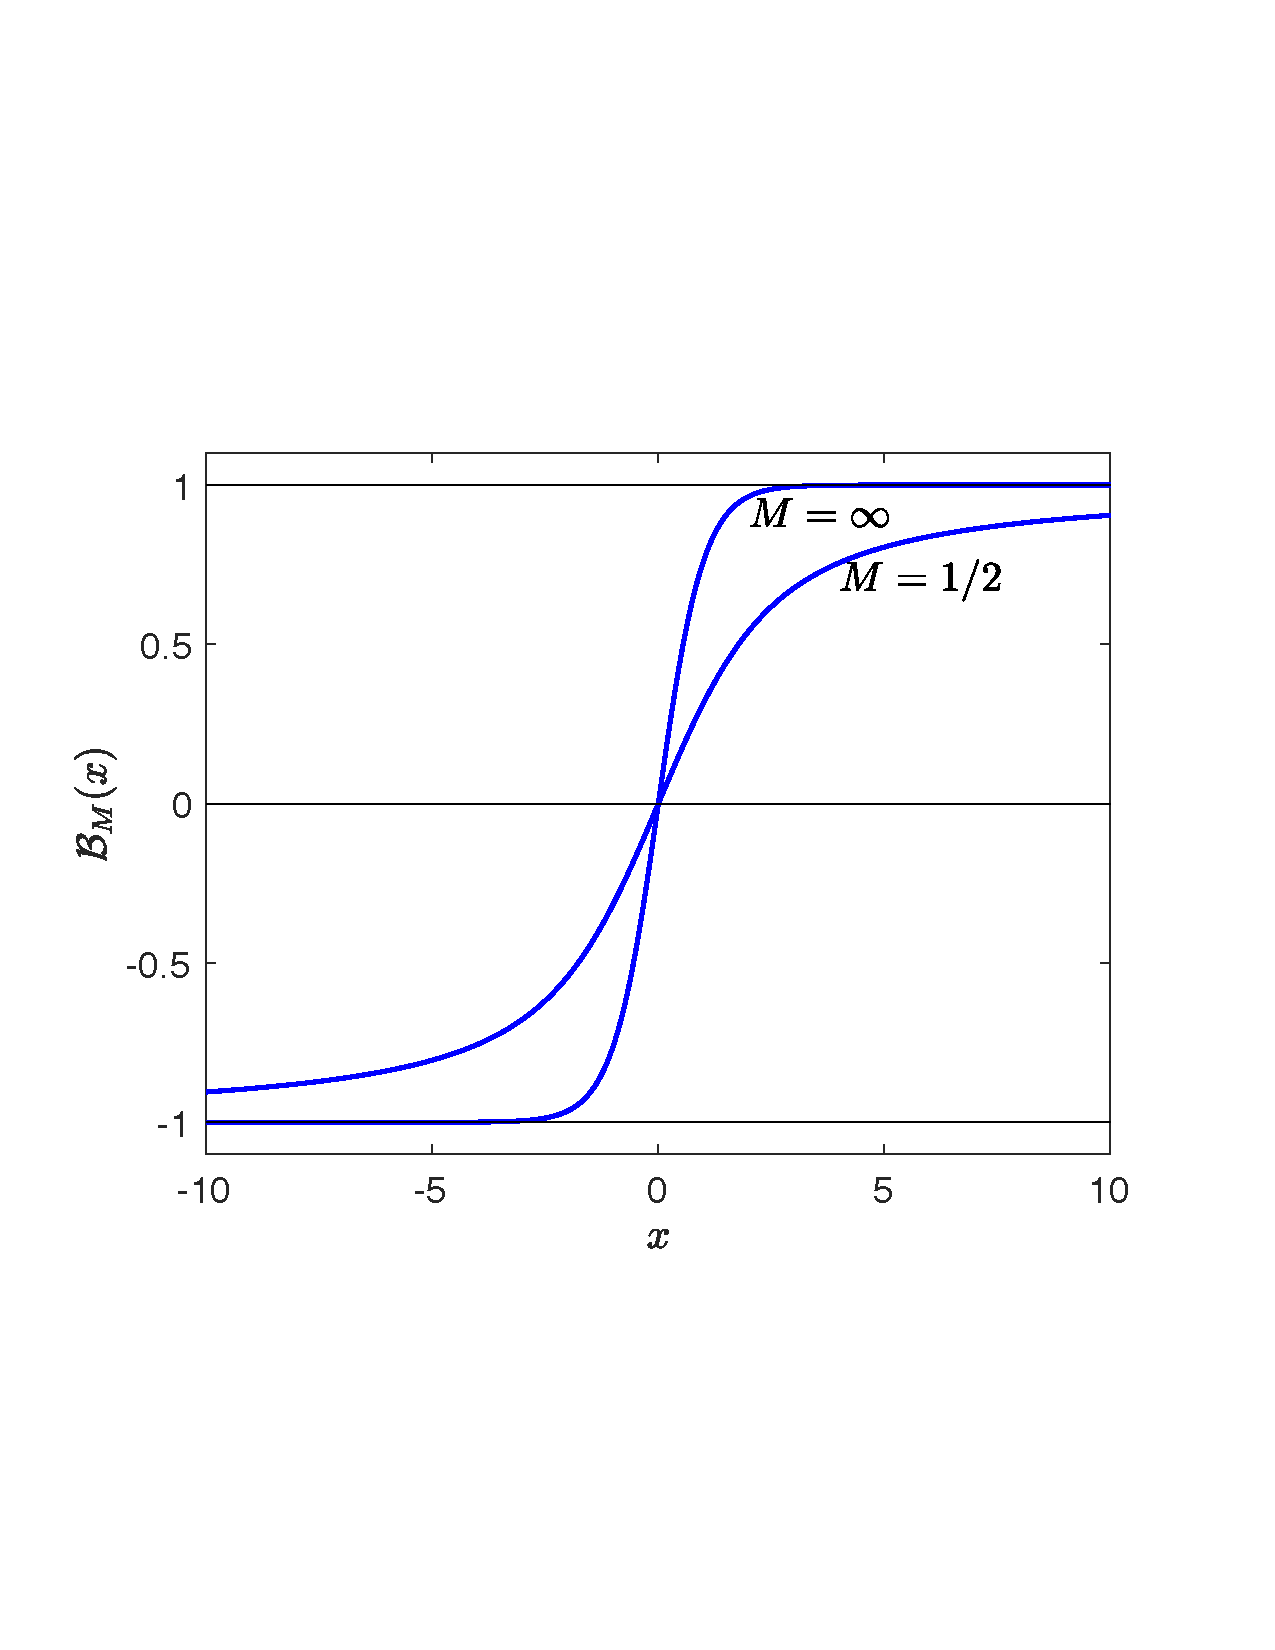
\includegraphics[width=7cm]{Brillouin}
\caption{Brillouin function for $M = 1/2$ and $M = \infty$.}
%\label{}
\end{center}
\end{figure}

%
This is the classical limit. 
%
\subsection{Strong spin-orbit coupling}
To avoid confusion we mark operators by hats.
If the spin-orbit coupling is strong compared to the magnetic field, then we cannot ignore the
spin-orbit term. In this case, $H$ still commutes with $L$ and $S$, 
but  no longer with $L^{z}$ and $S^{z}$. Instead, based on the relations
%
\newcommand{\vop}[1]{{\boldsymbol{ \hat #1}}}
\newcommand{\opp}[1]{ \hat {#1} }
\begin{align}
 \vop J &= \vop L + \vop S\\
\vop L\vop S &=\frac{1}{2}\bigg( \vop J^{2}-\vop L^{2}-\vop S^{2} \bigg)\;,\label{eq:para:2}
\end{align}
%
$H$ now commutes  with $L^{2},S^{2},J^{2},J_{z}$. The eigenvectors are therefore
%
\begin{align*}
\ket{\kappa,L,S,J,J_{z}}\;.
\end{align*}
%
The corresponding eigenvalues are given by  \eq{eq:H:spin:orbit:a} as
%
\begin{align*}
E(\kappa,L,S,J,J_{z}) &=E_{0}(\kappa,L,S) + \frac{B \mu_{B}}{\hbar}
\bigg(  J_{z} -\langle \opp S^{z} \rangle \bigg)\;.
\end{align*}
%
Here $\langle \opp S^{z} \rangle$ is the expectation value of of $\opp S^{z}$ in one of the eigenstates
$\ket{\kappa,L,S,J,J_{z}}$, while $J_{z}$ is already the eigenvalue of the operator $\opp J^{z}$.
%
The computation of the expectation value $\avg{\hat S_{z}}$ yields eventually 
%
\begin{align*}
E(\kappa,L,S,J,J_{z} &= E_{0}(\kappa,L,S) + \frac{\mu_{B}B}{\hbar}\underbrace{
\bigg(  1+  \frac{J(J+1)+S(S+1)-L(L+1)}{2 J(J+1)} \bigg)
}_{\color{blue} = g_{J}}J_{z}\\
&= E_{0}(\kappa,L,S) + \mu_{B}B g_{J} m\;,
\end{align*}
%
with $J_{z} = \hbar m$ and $m\in \{-J,-J+1,\dots,J\}$ 

\emphasize{prrof}{
To compute the expectation value we proceed as follows. 
We start out with the  identity
%
\begin{align}\label{eq:para:1}
\vop S \;\big( \vop  L\cdot \vop  S \big) -\big( \vop  L\cdot \vop  S \big)\;\vop  S
&=-i\hbar \vop  S \times \vop L\;.
\end{align}
%
which follows from
%
\begin{align*}
\opp S_{\nu} \;\opp L_{\mu}S_{\mu} - \opp L_{\mu}\opp S_{\mu} \opp S_{\nu} 
&=\opp S_{\nu} \;\opp S_{\mu} \;\opp L_{\mu}-\opp  S_{\mu} \;\opp S_{\nu}\;\opp L_{\mu}
=[\opp S_{\nu} ,\opp S_{\mu}]\;\opp L_{\mu}\\
&=i\hbar \varepsilon_{\nu\mu\rho} \opp S_{\rho} \opp L_{\mu} = -i\hbar \varepsilon_{\nu\rho\mu} \opp S_{\rho} \opp L_{\mu} \\
&=-i \hbar \big( \vop S\times \vop L \big)_{\nu}
\end{align*}\;.
%
%}
Next we multiply \eq{eq:para:1} with $\times \vop  J$ and obtain
%
\begin{align}\label{eq:para:2}
\vop S \;\big( \vop L\cdot \vop S \big)\times \vop J -\big( \vop L\cdot \vop S \big)\;\vop S\times \vop J
&=-i\hbar \big( \vop S\times \vop L \big)\times \vop J
\end{align}
%
Now, $\big( \vop L \cdot   \vop S \big)$ commutes with all components of the vector operator $\vop J$, since
according to \eq{eq:para:2} $\vop L\cdot\vop S$ is given by $\frac{1}{2}(\vop J^{2}-\vop L^{2}-\vop S^{2})$ 
which can be seen as follows
%
\begin{align*}
[\vop L\cdot\vop S,J^{\alpha}] &=
\frac{1}{2}\bigg(\underbrace{[J^{2},J^{\alpha}]}_{\color{blue} = 0}
-[L^{2},J^{\alpha}]-[S^{2},J^{a}]\bigg)\\
&=-\frac{1}{2}\bigg([L^{2},L^{\alpha}+S^{\alpha}]+[S^{2},L^{a}+S^{\alpha}]\bigg)\\
&=-\frac{1}{2}\bigg([L^{2},L^{\alpha}]+[S^{2},S^{\alpha}]\bigg)\\
&=0\;.
\end{align*}
%
Then we can move $\vop L\cdot \vop S$ in the first term of \eq{eq:para:2} to the right of $\vop J$,
resulting in 
%
\begin{align*}
\big(\vop S\times \vop J\big) \;\big( \vop L\cdot \vop S \big)- \big( \vop L\cdot \vop S \big)\;\big(\vop S\times \vop J\big)
&=-i\hbar \big( \vop S\times \vop L \big)\times \vop J
\end{align*}
If we now compute expectation values in the eigenvectors $\ket{\kappa,L,S,J,J_{z}}$, we can replace 
the operators $(\vop L\cdot \vop S)$ by the eigenvalues $\frac{1}{2}\big( J(J+1)-L(L+1)-S(S+1) \big)$ and the remaining expectation value on the left hand side is zero. Hence, we obtain from the right hand side
%
\begin{align}\label{eq:para:3}
\langle \big( \vop S\times \vop L \big)\times \vop J\rangle &= 0\;,
\end{align}
%
which is valid in the eigenstates.
From 
%
\begin{align*}
\big[ \big( \vop S\times \vop L \big)\times \vop J \big]_{i}
&= \varepsilon_{ijk}\big( \vop S\times \vop L \big)_{j} \opp J_{k}\\
&= \varepsilon_{ijk}\varepsilon_{jmn}  \opp S_{m} \opp L_{n} \opp J_{k}\\
&= \varepsilon_{jki}\varepsilon_{jmn}  \opp S_{m} \opp L_{n} \opp J_{k}\\
&= \big( \delta_{km}\delta_{in}-\delta_{kn}\delta_{im} \big)  \opp S_{m} \opp L_{n} \opp J_{k}\\
&= \opp S_{k} \opp L_{i} \opp J_{k}-\opp S_{i} \opp L_{k} \opp J_{k}\\
&= \opp  L_{i} \opp S_{k}\opp J_{k}-\opp S_{i} \opp L_{k} \opp J_{k}\;.
\end{align*}
%
we obtain for the double vector product
%
\begin{align*}
 \big( \vop S\times \vop L \big)\times \vop J &= \vop L\;\big( \vop S\cdot \vop J \big)
 -\vop S\;\big( \vop L\cdot \vop J \big)\\
&=\big( \vop J-\vop S\big)\;\big( \vop S\cdot \vop J \big)
 -\vop S\;\big( \vop L\cdot \vop J \big)\\
&= \vop J\;\big( \vop S\cdot \vop J \big)
 -\vop S\;\big( (\vop L+\vop S)\cdot \vop J \big)\\
 &= \vop J\;\big( \vop S\cdot \vop J \big)
 -\vop S\; \vop J^{2} \;.
\end{align*}
%

From \eq{eq:para:3} we therefore obtain
%
\begin{align*}
 \big( \vop S\times \vop L \big)\times \vop J 
 &= \vop J\;\big( \vop S\cdot \vop J \big)
 -\vop S\; \vop J^{2}  = 0\;.
\end{align*}
%
and for the expectation value in the  eigenstates  $ \ket{\kappa,L,S,J,J^{z}}$
we have
%
\begin{align*}
\avg{ \opp J_{z}\;\big( \vop S\cdot \vop J \big)} -  \avg{\opp  S_{z}\; J^{2} }&=0\;.
\end{align*}
%
Next we use
%
\begin{align*}
\vop S \cdot \vop J &= \vop S \cdot \vop L + \vop S^{2}\\
&=\frac{1}{2}\big( \vop J^{2}-\vop S^{2}-\vop L^{2} \big) + \vop S^{2}\\
&=\frac{1}{2}\big( \vop J^{2}+\vop S^{2}-\vop L^{2} \big) \;.
\end{align*}
and obtain
%
\begin{align*}
 J_{z}\;\frac{1}{2}\avg{ \vop J^{2}+\vop S^{2}-\vop L^{2}}-  \avg{ \opp S_{z}\; J(J+1) }&=0\\
  J_{z}\;\frac{1}{2}\;\big(J(J+1)+S(S+1)-L(L+1)\big) -  \avg{ \opp S_{z}}\; J(J+1)  &=0\;.
\end{align*}
%
%
The expectation value $\avg{S_{z}}$ in the eigenstates  $ \ket{\kappa,L,S,J,J^{z}}$
is therefore:
\begin{align*}
\langle S_{z}\rangle 
&=
J_{z}\; \frac{ J(J+1)+S(S+1)-L(L+1) }{2J(J+1)}\;.
\end{align*}
%
%
Hence, the eigenvalues are
%
\begin{align*}
E(\kappa,L,S,J,J_{z}) &= E_{0}(\kappa,L,S) + \frac{\mu_{B}B}{\hbar}\underbrace{
\bigg(  1+ \frac{1}{2}\big[ J(J+1)+S(S+1)-L(L+1) \big] \bigg)
}_{\color{blue} = g_{J}} J_{z}\;.
\end{align*}
%
}
The remaining calculation is similar to the previous one and one obtains
%
\begin{align*}
\frac{F}{N} 
&= E_{0}
-k_{B}T \ln\bigg(z_{J}\big(b\big) \bigg)
\end{align*}
%
with $b=g_{J}\mu_{B}\beta B$. Then
%
\begin{align*}
\vop M &= \vv e_{z} N J g_{J}\mu_{B}B\;{\cal B}_{J}(b J)\;.
\end{align*}
%

For high $T$ and small $B$, the susceptibility yields
\tboxit{Curie Law}{
%
\begin{align}
\chi_{\mu\nu} &=\delta_{\mu\nu} \frac{C}{T}\;.
\end{align}}
%
with 
%
\begin{align*}
C = \frac{N \mu_{0}\mu_{B}^{2}g_{J}^{2} J(J+1)}{3 k_{B}}\;,
\end{align*}
%
and for large $b$ we have
%
\begin{align*}
\frac{\vv M}{N}
&\underset{b\to\infty}{\longrightarrow} \pm  \vv e_{z} g_{J}\mu_{B}J \;.
\end{align*}

% \subsubsection{Plot of the Brillouin function}
%
\subsubsection{Entropy}
%
For the entropy we obtain
\begin{align*}
\frac{S}{N} &=-\pder{F/N}{T}{\vv B} = k_{B} \ln\big(z_{J}(b)\big)
+k_{B}T \frac{z'_{J}(b)}{z_{J}(b)} \frac{d b}{dT}\\
\end{align*}
%
%
\begin{align*}
 \frac{d b}{dT} &=  -g_{J}\mu_{B} B \frac{1}{k_{B}T^{2}}
 = -\beta^{2} g_{J}\mu_{B} B = - \beta b\;.
\end{align*}
%
\begin{align*}
S &= k_{B} \bigg(\ln\big(z_{J}(b)\big)
-b\frac{z'_{J}(b)}{z_{J}(b)} \bigg)\\
\end{align*}
Along with \eq{eq:para:8} we obtain
\begin{align*}
\frac{S}{N} &= k_{B} \bigg(\ln\bigg(
\frac{\sinh(b (J+1/2))}{\sinh(b/2)}
\bigg)
-b J{\cal B}_{J}(b J) \bigg)\;.
\end{align*}
For  $b \ll 1$ (i.e. $T\to \infty$) we find 
%
\begin{align*}
\frac{S}{N} &=  k_{B} \bigg(\ln\bigg(
\frac{b(J+1/2)}{b/2}
\bigg)
-(b J)^{2} \frac{J+1}{3J}\; \bigg)\\
&=k_{B} \ln\big(2J+1\big)\;.
\end{align*}
%
The argument is the number of eigenvalues of $J_{z}$.
\subsection{Plot of $S$ and specific heat}

In \autoref{fig:magnetism-entropy} the before obtained entropy per particle $\frac{S}{N}$ is depicted. Note also that for $b \ll 1$ we can now check visually that $\frac{S}{N} \to k_B \ln(2J+1)$.

Additionaly, the heat capacity is shown as it is connected to the entropy by:

\begin{align*}
  C_V &= T\frac{\partial S}{\partial T} = T \frac{\partial S}{\partial b} \frac{\partial b}{\partial T} = T \frac{\partial S}{\partial b} \frac{\partial}{\partial T} \frac{B\mu_B}{k_B T} \\ 
  C_V &= T \frac{\partial S}{\partial b} \left(-\frac{B\mu_B}{k_BT^2}\right) = \frac{\partial S}{\partial b} \left(-\frac{B\mu_B}{k_B T}\right)   \\
  C_V &= -b \frac{\partial S}{\partial b}
\end{align*}

\begin{figure}[htbp]
  \begin{center}
  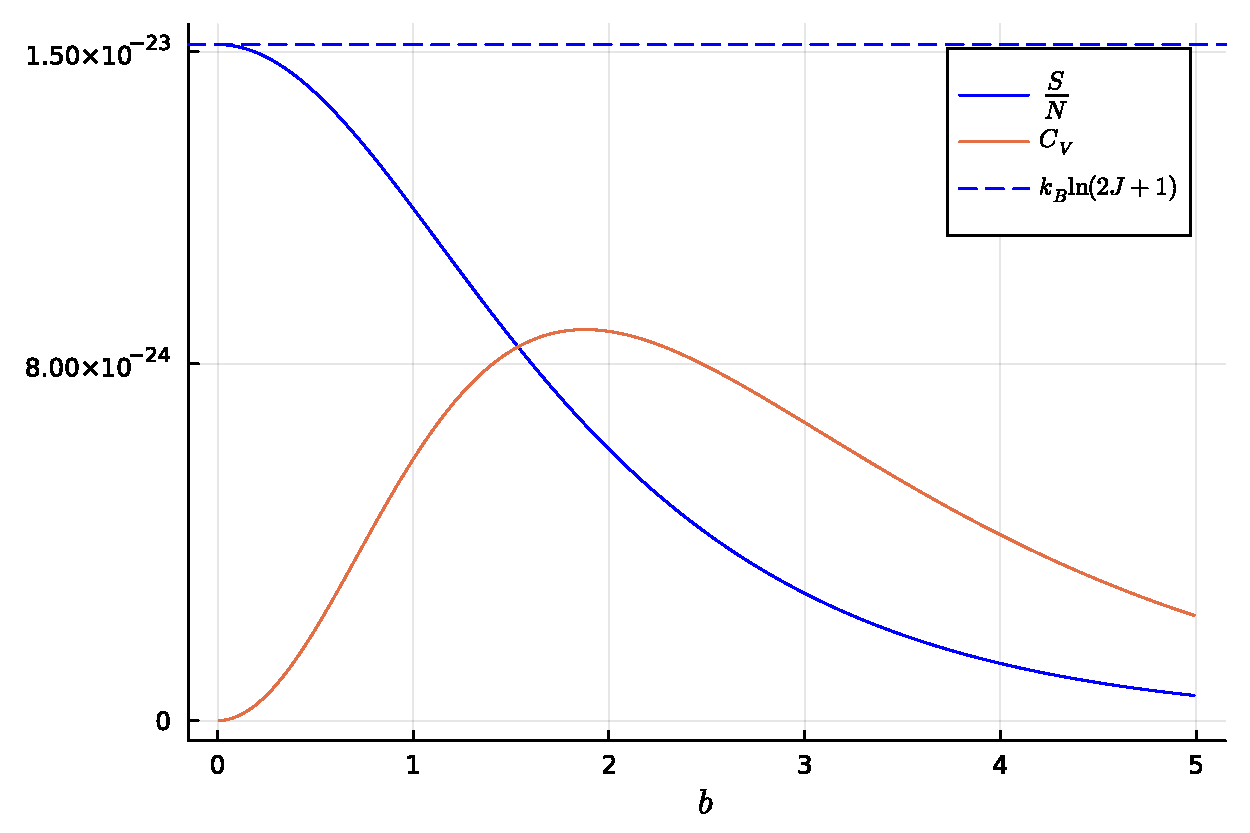
\includegraphics[width=0.8\textwidth]{magnetism_entropy.pdf}
  \caption{Entropy and specific heat for strong spin-orbit coupling and $J=1$.}
  \label{fig:magnetism-entropy}
  \end{center}
\end{figure}
  %
\section{Magnetism of the free electron model}
The free electron gas is based on the following assumptions: no electron-electron interactions, 
the electrons experience no potential due to the crystal, they  are confined to a box. In addition,
we apply a constant homogeneous external magnetic field. 


\subsection{Pauli paramagnetism}

First, we restrict the discussion to the coupling of the electronic spin to the magnetic field, i.e.
we ignore the angular momentum.
The energy one-particle eigenvalues are
%
\begin{align*}
\varepsilon_{\sigma}(\vv k) &= \frac{\hbar^{2} \vv k^{2}}{2m} +\sigma b\;,\\
b &= \frac{\mu_{B} g_{e} }{2}B\;.
\end{align*}
%
with the quantized wave vectors $\vv k$.
The mean occupation of the one-particle orbitals is given by the Fermi-Dirac distribution
%
\begin{align*}
n_{F}(\varepsilon_{\sigma}(\vv k)|T,\mu)
\end{align*}
%
The mean total number of electrons in the Zeeman level represented by $\sigma$ is
%
\begin{align*}
N_{\sigma} &=\sum_{\vv k} n_{F}(\varepsilon_{\sigma}(\vv k)|T,\mu)
= \int d\varepsilon \rho(\varepsilon) n_{F}(\varepsilon +\sigma b|T,\mu)\;.
\end{align*}
%
As derived in \app{app:dos} the 3D dos is
%
%
\begin{subequations}\label{eq:para:pauli:1}
\begin{align}
\rho(\varepsilon)&= D \sqrt{\varepsilon}\;,\\
\text{with}\quad D&=\frac{V m^{3/2}}{\hbar^{3} \pi^{2}\sqrt{2}}\;.
\end{align}
\end{subequations}
%
Then
%
\begin{align*}
N_{\sigma} &=D\;
\int_{0}^{\infty} d\varepsilon \sqrt{\varepsilon} \; n_{F}(\varepsilon +\sigma b|T,\mu)\;.
\end{align*}
%
For small magnetic field we can use a Taylor expansion in $b$ abound $b=0$
%
\begin{align*}
N_{\sigma} &=D\;
\int_{0}^{\infty} d\varepsilon \sqrt{\varepsilon} \; 
\bigg(n_{F}(\varepsilon|T,\mu) +\sigma b \;\frac{\partial }{\partial \varepsilon}n_{F}(\varepsilon|T,\mu) +{\cal O}(b^{2})\bigg)\\
 &=D\;
\int_{0}^{\infty} d\varepsilon \sqrt{\varepsilon} \; 
n_{F}(\varepsilon|T,\mu) 
+\sigma b D \int_{0}^{\infty} d\varepsilon \sqrt{\varepsilon} \;n'_{F}(\varepsilon|T,\mu) +{\cal O}(b^{2})
\end{align*}
%
By now plugging in $\sigma = \pm 1$ and adding $N_{+1}$ and $N_{-1}$ together, the term depending on $\sigma$ cancels out and only the first term is left. Hence, the total particle number follows as:
 %
\begin{align}
N &= N_{+}+N_{-} = 2 D \int_{0}^{\infty} d\varepsilon \sqrt{\varepsilon} \;n_{F}
(\varepsilon|T,\mu) +
{\cal O}(b^{2})\notag\\
&= 2 D \int_{0}^{\infty} d\varepsilon \sqrt{\varepsilon} \;n_{F}
(\varepsilon|T,\mu) +
{\cal O}(b^{2})\;.\label{eq:N:total}
\end{align}
%
For small $b$ and low temperature we can use the Sommerfeld expansion, outlined in \app{Sommerfeld},
%
\tboxit{Sommerfeld expansion}{
\begin{align}\label{eq:}
I&=\int_{0}^{\infty}  f(\varepsilon) n_{F}(\varepsilon|\mu,T) d\varepsilon\nonumber\\
 &=\int_{0}^{\mu} f(\varepsilon)d\varepsilon
+ 2  \sum_{n=1}^{\text{odd}}\left(1-\frac{1}{2^{n}}\right)\;\zeta(n+1)
\big(k_{B}T\big)^{n+1}\;f^{(n)}(\mu)\;,
\end{align}}
%
which reads to leading order using $\zeta(2) = \frac{\pi^2}{6}$:
%
\begin{align*}
I &= \int_{0}^{\mu} f(\varepsilon) d\varepsilon +  \frac{\pi^{2}}{6}\;\big(k_{B}T\big)^{2} \;f'(\mu)+ {\cal O}\bigg(\bigg(\frac{k_{B}T}{\mu}\bigg)^{4}\bigg)\;.
\end{align*}
%
For the total particle number we obtain
\begin{align*}
N&=2 D \bigg(\int_{0}^{\mu}\sqrt{\varepsilon} ~d\varepsilon
+\frac{\pi^{2}}{6}\frac{d}{d\mu}\sqrt{\mu}\bigg( k_{B}T \bigg)^{2}+\ldots\bigg)\\
&=2 D \bigg(\frac{2}{3}\mu^{3/2} 
+\frac{\pi^{2}}{12}\mu^{-1/2}\big( k_{B}T \big)^{2}+\ldots
\bigg)\;.
\end{align*}
%
%
\begin{align}\label{eq:spin:para:aux2}
\frac{3 N}{4 D}&= \mu^{3/2}\bigg(1
+\frac{\pi^{2}}{8}\bigg(\frac{ k_{B}T }{\mu}\bigg)^{2}+\ldots
\bigg)
\end{align}
%

%
For $T=0$ the chemical potential is equivalent to the Fermi energy $\varepsilon_{F}$ and we have
%
\begin{align}\label{eq:spin:para:aux1}
\frac{3 N}{4 D} &= \varepsilon_{F}^{3/2}\;,
\end{align}
%
or rather
%
\begin{align*}
\varepsilon_{F} 
&=  \bigg(\frac{3 N \hbar^{3}  (2\pi)^{2} }{4 V(2m)^{3/2}} \bigg)^{2/3}
=  \bigg(\frac{3 N   \pi^{2} }{ V} \bigg)^{2/3}\;\frac{\hbar^{2}}{2 m}\;.
\end{align*}
%
\tboxit{Fermi energy in the free electron gas}{
\begin{align}\label{eq:spin:para:EF}
\varepsilon_{F}&=  \bigg(3  \pi^{2} n\bigg)^{2/3}
\frac{\hbar^{2}}{2m} \;.
\end{align}}
%
This defines the Fermi wave number $k_{F}$, through
%
\begin{align*}
\varepsilon_{F} &
= \bigg(3  \pi^{2} n\bigg)^{2/3}\frac{\hbar^{2}}{2m} 
= \frac{\hbar^{2}	k_{F}^{2} }{2m}\\
k_{F}&=\bigg(3  \pi^{2} n\bigg)^{1/3} = \bigg(\frac{3 \pi^{2}}{v}\bigg)^{1/3 }\;,
\end{align*}
%
where $v$ is the average volume per electron. Hence 
%
\begin{align*}
k_{F} &\propto \frac{1}{r}\;,
\end{align*}
%
where $r$ is the mean distance between the electrons.
Inserting \eq{eq:spin:para:aux1} in \eq{eq:spin:para:aux2} yields apart from higher order terms
%
\begin{align*}
\varepsilon_{F}
&= \mu\bigg(1 +\frac{\pi^{2}}{8}\bigg(\frac{ k_{B}T }{\mu}\bigg)^{2}\bigg)^{2/3}\\
\mu &= \varepsilon_{F}\bigg(1 +\frac{\pi^{2}}{8}\bigg(\frac{ k_{B}T }{\mu}\bigg)^{2}\bigg)^{-2/3}\;.
\end{align*}
%
We can solve this equation iteratively, starting with 
$\mu=\varepsilon_{F}$. The first iteration yields
%
\begin{align*}
\mu &=\varepsilon_{F}\bigg(1 +\frac{\pi^{2}}{8}\bigg(\frac{ k_{B}T }{\varepsilon_{F}}\bigg)^{2}\bigg)^{-2/3}\;.
\end{align*}
%
For low temperatures, 
$\frac{ k_{B}T }{\varepsilon_{F}}<1$ we can as well write
\begin{align*}
\mu &=\varepsilon_{F}\bigg(1 -\frac{\pi^{2}}{8}\frac{2}{3}\bigg(\frac{ k_{B}T }{\varepsilon_{F}}\bigg)^{2} +{\cal O}\bigg( \bigg( \frac{k_{B}T}{\varepsilon_{F}} \bigg)^{4} \bigg)\bigg)\;.
\end{align*}
%
Further iterations do not change the second order term and we generally have
%
\tboxitp{Chemical potential}{free electron gas}{
\begin{align}\label{eq:}
\mu &=\varepsilon_{F}\bigg(1 -\frac{\pi^{2}}{12}\bigg(\frac{ k_{B}T }{\varepsilon_{F}}\bigg)^{2} \bigg)\;+{\cal O}\bigg( \bigg( \frac{k_{B}T}{\varepsilon_{F}} \bigg)^{4} \bigg)
\end{align}}
%

%

%
The partition function for non-interacting particles has already been derived previously.
For one-particle energies $\varepsilon_{\nu}$ it was
%
\begin{align*}
\ln(Z) &= \sum_{\nu} \ln\bigg( 1+  e^{-\beta(\varepsilon_{\nu}-\mu)}\bigg)\;.
\end{align*}
%
In the present case the index $\nu$ stands for the wave vector $\vv k$ and the spin direction. Hence
%
\begin{align}\label{eq:para:pauli:ln:Z}
\ln(Z) 
%&= \sum_{\sigma} \sum_{\vv k} \ln\bigg( 1+  e^{-\beta(\varepsilon(\vv k)+\sigma b-\mu)}\bigg)\\
&= \sum_{\sigma} \int_{0}^{\infty}\;\rho(\varepsilon)\;
\ln\bigg( 1+  e^{-\beta(\varepsilon+\sigma b-\mu)}\bigg)\;.
\end{align}
%

The corresponding grand  potential reads
%
\begin{align*}
\Omega(T,\vv B) &= -k_{B}T \ln(Z) =-k_{B}T   \sum_{\sigma} \int_{0}^{\infty}\;\rho(\varepsilon)\;
\ln\bigg( 1+  e^{-\beta(\varepsilon+\sigma b-\mu)}\bigg)\;.
\end{align*}
%
The magnetization in z-direction is obtain via
%
\begin{align*}
M &= - \pder{\Omega}{B}{T} \\
&=k_{B}T\;\sum_{\sigma}\big( -\frac{\beta\sigma \mu_{B}g_{e}}{2} \big)
\int_{0}^{\infty} d\varepsilon\;\rho(\varepsilon)\;\frac{e^{-\beta(\varepsilon+\sigma b-\mu)}}{1+e^{-\beta(\varepsilon+\sigma b-\mu)}}\\
&=-\frac{\mu_{B}g_{e}}{2} \;\sum_{\sigma}\sigma \;\;
\int_{0}^{\infty} d\varepsilon\;\rho(\varepsilon)\;n_{F}(\varepsilon+\sigma b|T,\mu)\\
&= -\frac{\mu_{B}g_{e}}{\hbar} \;\underbrace{
 \frac{\hbar(N_{+}-N_{-})}{2}
}_{\color{blue} = \langle S_\text{total}^{z} \rangle}
\end{align*}
%
In agreement with \eq{eq:magmo:spin}. Again we assume that $b$ is small and 
employ a Taylor expansion. 
%
\begin{align*}
M &= -\frac{\mu_{B}g_{e} }{2} \sum_{\sigma} \sigma \int_{0}^{\infty}d\varepsilon \bigg(\rho(\varepsilon) n_{F}(\varepsilon|T,\mu) + \sigma b n'_{F}(\varepsilon|T,\mu)+{O}(b^{2})\bigg)\\
&= -\frac{\mu_{B}g_{e} }{2} 2b \int_{0}^{\infty}d\varepsilon \rho(\varepsilon)  n'_{F}(\varepsilon|T,\mu)+{O}(b^{2})\\
&= -\frac{(\mu_{B}g_{e})^{2} }{2}  B\int_{0}^{\infty}d\varepsilon \rho(\varepsilon)  n'_{F}(\varepsilon|T,\mu)+{O}(b^{2})\;.
\end{align*}
%
Then the susceptibility reads
%
\begin{align}
\chi_{T} &= \mu_{0}\pder{M}{B}{T}\bigg|_{B=0}\notag\\
&=-\mu_{0}\frac{(\mu_{B}g_{e})^{2} }{2}  \int_{0}^{\infty}d\varepsilon \rho(\varepsilon)  n'_{F}(\varepsilon|T,\mu)\notag\;.
\end{align}
%
This can also be written as
%
\begin{align*}
\chi_{T} &= -\mu_{0} \mu_{B}^{2} \bigg(\frac{g_{e}}{2}\bigg)^{2} 2 
\int d\varepsilon \rho(\varepsilon) n'_{F} (\varepsilon|T,\mu)\\
&= \mu_{0} \mu_{B}^{2} \bigg(\frac{g_{e}}{2}\bigg)^{2} 2 
\frac{\partial }{\partial \mu} 
\int d\varepsilon \rho(\varepsilon) n_{F} (\varepsilon|T,\mu)\;.
\end{align*}
%
Comparison with \eq{eq:N:total} yields 
\begin{align}\label{eq:Pauli:dN:dmu}
\chi_{T} 
&= \mu_{0} \mu_{B}^{2} \bigg(\frac{g_{e}}{2}\bigg)^{2} 
\pder{N}{\mu}{T,B=0}
\end{align}

We use the Sommerfeld expansion, derived in \app{Sommerfeld} to expand the integral in powers of $k_{B}T/\mu$. 
%
\begin{align*}
\chi &=-\mu_{0}\frac{(\mu_{B}g_{e})^{2} }{2}  \int_{0}^{\infty}d\varepsilon \rho(\varepsilon)  n'_{F}(\varepsilon|T,\mu)\notag\\
&=\mu_{0}\frac{(\mu_{B}g_{e})^{2} }{2}  \int_{0}^{\infty}d\varepsilon \rho'(\varepsilon)  n_{F}(\varepsilon|T,\mu)\\
 &=\mu_{0}\frac{(\mu_{B}g_{e})^{2} }{2}  \bigg(\int_{0}^{\mu}d\varepsilon \rho'(\varepsilon)
+\frac{\pi^{2}}{6}(k_{B}T)^{2}\rho''(\mu)+ {\cal O}(\big(\frac{k_{B}T}{\mu}\big)^{4})
 \bigg)\\    
  &=\mu_{0}\frac{(\mu_{B}g_{e})^{2} }{2}  \bigg( \rho(\mu)
+\frac{\pi^{2}}{6}(k_{B}T)^{2}\rho''(\mu)+ {\cal O}(\big(\frac{k_{B}T}{\mu}\big)^{4})
 \bigg)\;.
\end{align*}
%
The final result reads
%
\begin{align}\label{eq:para:chi}
\chi   &=\mu_{0}\frac{(\mu_{B}g_{e})^{2} }{2}  \rho(\mu)\bigg( 1
+\frac{\pi^{2}}{6}(k_{B}T)^{2}\frac{\rho''(\mu)}{\rho(\mu)}+\ldots
 \bigg)
\end{align}
%
Now we recall, that $\rho(\varepsilon) = D \sqrt{\varepsilon}$, resulting in
$\rho''(\mu)/\rho(\mu)=-1/(4\mu^{2})$. 
%
\tboxitp{Magnetic susceptibility}{free electron gas}{
\begin{align}
\chi_{P} &= \mu_{0}\frac{(\mu_{B}g_{e})^{2} }{2}  \rho(\mu)
\bigg( 1 - \frac{\pi^{2}}{24}\bigg(\frac{k_{B}T}{\mu}\bigg)^{2} +\ldots\bigg)\;.
\end{align}}
%
We see that indeed $k_{B}T/\mu$ is the relevant small parameter.
This describes the \red{Pauli-spin-paramagnetism}, which is almost temperature
independent for low $T$; in strong contrast to the Curie $1/T$ behaviour.
The reason for the discrepancy lies in the fermi-statistics. Only the spin of the electrons in the vicinity of $\mu$ can contribute. The number of thermally excited electrons
is $k_{B} T \rho(\mu)$ which compensates the $1/T$ behaviour.


\subsection{Landau diamagnetism}
So far we have only considered the spin degrees of freedom of the free electron gas. The orbital moments also contribute to the magnetization, which results in the Landau diamagnetism.

The single electron energies are now
%
\begin{align*}
\varepsilon_{n,\sigma}(k_{z}) &=\varepsilon(k_{z})
+\hbar \omega_{c} (n+\tfrac{1}{2}) + \sigma b\\
\varepsilon(k_{z}) &=\frac{\hbar^{2} k_{z}^{2}}{2m}
\end{align*}
%
with $b=\frac{\mu_{B} g_{e}}{2}$ and the cyclotron frequency $\omega_{c} = \frac{e B}{m}$, and $\mu_{B} = \frac{e \hbar}{2m}$.  
The degeneracy of these levels is 
%
\begin{align*}
N_\text{deg} &= \frac{L_{x}L_{y} e B}{2 \pi \hbar} = B C_{deg}\;.
\end{align*}
%
We use again the formula for the grand canonical partition function of non-interacting particles 
%
\begin{align*}
\ln(Z)
&= \sum_{\nu} \ln\big( 1+^{-\beta(\varepsilon_{\nu}-\mu)} \big)
\end{align*}
%
Inserting the one particle energies results in
%
\begin{align}
\ln(Z)
&= B C_{deg}\sum_{\sigma} \sum_{n=0}^{\infty}\underbrace{
\int d\varepsilon\rho^{(1d)}(\varepsilon)
\ln\bigg( 1+e^{-\beta(\varepsilon + \hbar \omega_{c}(n+\tfrac{1}{2}) + b\sigma-\mu)} \bigg)
}_{\color{blue} := \underbrace{
F(\mu - \hbar \omega_{c}(n+\tfrac12) -b\sigma)
}_{\color{blue} := f(n+\tfrac12)}}\;.
\end{align}
%
Now we invoke the leading Euler-Mac-Laurin formula (see \autoref{app:Euler:MacLaurin}) in \eq{eq:Euler:MacLaurin} to leading order 
and use $f'(\infty)=0$.
%
\begin{align*}
\sum_{n=0}^{\infty} f(n+\tfrac12) &= \int_{0}^{\infty} f(x) dx
+\frac{1}{24} f'(0) +\ldots\\
&=\int_{0}^{\infty} F(\mu-\hbar \omega_{c} x -b \sigma ) dx
+\frac{1}{24}\frac{\partial }{\partial x} F(\mu-\hbar \omega_{c} x -b \sigma )\bigg|x=0 +\ldots\\
&=\frac{1}{\hbar \omega_{c}}\int_{0}^{\infty} F(\mu-y -b \sigma) dy
-\frac{\hbar \omega_{c}}{24}\frac{\partial }{\partial \mu} F(\mu-b \sigma ) +\ldots\;.
\end{align*}
%
Next we expand this expression in terms of $B$, or rather $b$, up to second order. We also include already the sum over the electronic spin, which allows to omit term proportional to $\sigma^{m}$ for odd $m$.
%
\begin{align*}
\sum_{\sigma} \sum_{n} f(n+\tfrac12) &=\sum_{\sigma}
\frac{1}{\hbar \omega_{c}} 
\bigg(
\int_{0}^{\infty} F(\mu-y)dy - \canceled{b \sigma} \int_{0}^{\infty} \frac{\partial }{\partial \mu}F(\mu-y)dy +\\
&\quad + \frac{b^{2}}{2}\int_{0}^{\infty} \frac{\partial^{2} }{\partial \mu^{2}}F(\mu-y)dy
 -\frac{(\hbar \omega_{c})^{2}}{24}\frac{\partial }{\partial \mu} 
 F(\mu)   
 +{\cal O}(B^{4})\bigg)\\
 %=========
 &=
\frac{2}{\hbar \omega_{c}} 
\bigg(
\int_{-\infty}^{\mu} F(z)dz  +\\
&\quad + \frac{b^{2}}{2}\int_{0}^{\infty} \frac{\partial^{2} }{\partial y^{2}}F(\mu-y)dy
 -\frac{(\hbar \omega_{c})^{2}}{24}\frac{\partial }{\partial \mu}  F(\mu)   
 +{\cal O}(B^{4})\bigg)\\
  &=
\frac{2}{\hbar \omega_{c}} 
\bigg(
\int_{-\infty}^{\mu} F(z)dz  +\\
&\quad + \frac{b^{2}}{2}\big(\frac{\partial }{\partial \mu}F(\mu-y)\big)\bigg|_{y=0}^{y=\infty}
 -\frac{(\hbar \omega_{c})^{2}}{24}\frac{\partial }{\partial \mu}  F(\mu)   
 +{\cal O}(B^{4})\bigg)\\
   &=
\frac{2}{\hbar \omega_{c}} 
\bigg(
\int_{-\infty}^{\mu} F(z)dz 
 +\frac{1}{2}\big( b^{2}-\frac{(\hbar \omega_{c})^{2}}{12}\big)
 \frac{\partial }{\partial \mu}F(\mu)
 +{\cal O}(B^{4})\bigg)\;.
\end{align*}
%
Inserting the definition of $\omega_{c}$ and $b$
yields
%
\begin{align*}
b^{2} -\frac{\big(\hbar \omega_{c}\big)^{2}}{12} 
&=B^{2}\bigg( \mu_{B}^{2}\bigg(\frac{g_{e}}{2}\bigg)^{2} - \frac{1}{12}\bigg(\frac{\hbar e}{m}\bigg)^{2} \bigg)\\
&=B^{2}\mu_{B}^{2}\bigg( \bigg(\frac{g_{e}}{2}\bigg)^{2} - \frac{4}{12} \bigg)\\
\end{align*}
%
The grand potential up to order $B^{2}$ reads 
%
\begin{align*}
\Omega &= -k_{B}T \ln(Z)\\
&=\underbrace{-
\frac{2 k_{B} T C_{deg}B}{\hbar \omega_{c}} 
}_{\color{blue} = D}
\bigg(
\int_{0}^{\infty} F(\mu-y)dy  
 +\frac{\mu_{B}^{2}B^{2}}{2}\bigg(  \bigg(\frac{g_{e}}{2}\bigg)^{2} - \frac{4}{12}  \bigg)
 \frac{\partial }{\partial \mu}F(\mu)\bigg)\\
 &=
D  \int_{0}^{\infty} F(\mu-y)dy  
 +\frac{1}{2}\bigg(  \bigg(\frac{g_{e}}{2}\bigg)^{2} - \frac{4}{12}  \bigg)
\;D \frac{\partial }{\partial \mu} F(\mu)\;.
\end{align*}
%
For $B=0$ we obtain
%
\begin{align*}
\Omega(T,\mu,B=0) &= D  \int_{0}^{\infty} F(\mu-y)dy 
\end{align*}
%
We can exploit
%
\begin{align*}
\frac{\partial }{\partial \mu} \int_{-\infty}^{\mu} F(z)dz &= F(\mu)\\
\Rightarrow\qquad  \frac{\partial }{\partial \mu}F(\mu) &= \frac{\partial^{2} }{\partial \mu^{}2} \int_{-\infty}^{\mu} F(z)dz 
\end{align*}
%
to rewrite  the grand potential as
%
\begin{align*}
\Omega(T,\mu,B) &= \Omega(T,\mu,B=0) +
\frac{\mu_{B}^{2}B^{2}}{2}\bigg(  \bigg(\frac{g_{e}}{2}\bigg)^{2} - \frac{1}{3}  \bigg)
 \frac{\partial^{2} }{\partial \mu^{2}}\Omega(T,\mu,B=0)\;.
\end{align*}
%
The susceptibility is defined as 
%
\begin{align*}
\chi&= -\frac{\partial \Omega}{\partial B^{2}}\bigg|_{\mu,T} = 
-\mu_{B}^{2}\bigg(  \bigg(\frac{g_{e}}{2}\bigg)^{2} - \frac{1}{3}  \bigg)
 \frac{\partial^{2} }{\partial \mu^{2}}\Omega(T,\mu,B=0)\;,
\end{align*}
%
Finally, we exploit the equation  $\pder{\Omega}{\mu}{T,B}=N(T,\mu,B)$ resulting in
\begin{align*}
\chi&= -\frac{\partial \Omega}{\partial B^{2}}\bigg|_{\mu,T} = 
 \bigg(  1 - \frac{1}{3} \bigg(\frac{2}{g_{e}}\bigg)^{2} \bigg)
\bigg(\mu_{B}^{2}\bigg(\frac{g_{e}}{2}\bigg)^{2}  \frac{\partial }{\partial \mu}N(T,\mu,B=0)\bigg)\;,
\end{align*}


According to \eq{eq:Pauli:dN:dmu} the last bracket is equal to the Pauli-spin susceptibility, i.e.

\begin{align*}
\chi&= 
\chi_{P} - \frac{1}{3} \bigg(\frac{2}{g_{e}}\bigg)^{2} \chi_{P}
\end{align*}

The additional term is called {\em Landau diamagnetism} and for $g_{e}\approx 2$ is 
is
%
\begin{align*}
\chi_{L}&=-\frac{1}{3} \chi_{P}
\end{align*}
%
The total susceptibility is still positive 
%
\begin{align*}
\chi &\approx \frac{2}{3} \chi_{P}\;.
\end{align*}
%

\tboxitp{Landau Diamagnetism}{free electron gas}{
%
\begin{align}\label{eq:}
\chi_{L}&= -\frac{1}{3}\chi_{P}
\end{align}
%
}

\section{Collective magnetism }

\subsection{Heisenberg hamiltonian}
In many crystaline  systems, the electrons can be split into those that are localized at the atomic sites and others which can move freely through the crystal. The former result in localized
magnetic moments or spins $\vv S_{i}$, if they do not belong to closed shells. 
We have discussed these  local spins $\vv S_{i}$ before, but there we have focussed on systems where these spins do not interact. 
The Coulomb interaction between the electrons can lead to various types of exchange interactions
between these spins. The exchange can either result from exchange processes of the electrons that form the local spins on neighboring sites {\em direct exchange} or it can be mediated by
additional electrons {\em indirect exchange}. In the latter case, the interaction can be long ranged, like in the case of the so-called {\em RKKY} (Ruderman-Kittel-Kasuya-Yosida). 
In RKKY the interaction decays like $1/\abs{\vv R_{i}-\vv R_{j}}^{3}$ with the distance between the spins at site 
$\vv R_{i}$ and $\vv R_{j}$. In addition, the exchange interaction  changes sign as function of distance, i.e.
depending on the distance between the localized spins it can be ferromagnetic and anti-ferromagnetic. In all cases, the interaction can be described by a prominent model for collective magnetism, the 
\tboxit{Heisenberg model}{
\begin{align}\label{eq:}
H &= - \sum_{jj'}
\bigg( J^{z}_{jj'} S^{z}_{j}   S^{z}_{j'}+  J^{xy}_{jj'} 
\big(S^{x}_{j}   S^{x}_{j'}+ S^{y}_{j}   S^{y}_{j'}\big)
\bigg) 
+ b \sum_{j} S^{z}_{j}\;.
\end{align}
}
Here $J_{jj'} = J((\vv R_{j}-\vv R_{j'}))$, with $J_{jj}=0$.
 $J_{jj'}$ can always be chosen symmetric, since by substituting $j\leftrightarrow j'$ we find
%
\begin{align*}
H_{H}= -\sum_{\alpha}\sum_{jj'} J_{jj'} S^{\alpha}_{j}S^{\alpha}_{j'} &= -\sum_{\alpha}\sum_{jj'} J_{j'j} S^{\alpha}_{j'}S^{\alpha}_{j} =-\sum_{\alpha}\sum_{jj'} J_{j'j} S^{\alpha}_{j}S^{\alpha}_{j'} 
\end{align*}
%
Hence 
%
\begin{align*}
H &= \frac{1}{2}\bigg(  -\sum_{\alpha}\sum_{jj'} J_{jj'} S^{\alpha}_{j}S^{\alpha}_{j'} 
 -\sum_{\alpha}\sum_{jj'} J_{j'j} S^{\alpha}_{j}S^{\alpha}_{j'}  \bigg)=
 -\sum_{\alpha}\sum_{jj'} \bigg(\frac{J_{jj'}+J_{j'j}}{2}\bigg) S^{\alpha}_{j}S^{\alpha}_{j'} \;.
\end{align*}
%
We also introduce the ladder operators
%
\begin{align}\label{eq:}
S_{j}^{\pm} &= S_{j}^{x}\pm i S_{j}^{y}\;.
\end{align}
%
In these operators, the hamiltonian reads
\begin{align*}
H &= - \sum_{jj'} \bigg( J^{z}_{jj'} S_{j}^{z}  S_{j'}^{z}
+J_{jj'}^{xy}S_{j}^{+} S_{j'}^{-}
\bigg) + b \sum_{j} S^{z}_{j}\;.
\end{align*}
%
The order of the operators $S_{j}^{+}S_{j'}^{-}$ is irrelevant, since $j\ne j'$ and in that case they commute.
There are three important limiting cases depending on the anisotropy of the crystal in spin-space.
\begin{itemize}
	\item ($\abs{J^{z}}\ll\abs{J^{xy}}$) results in the so-called {\em xy- model}
\tboxit{xy-model}{
\begin{align}
H &= - \sum_{jj'} 
J_{jj'}^{xy}S_{j}^{+} S_{j'}^{-}
 + b \sum_{j} S^{z}_{j}\;.
\end{align}}

\item ($\abs{J^{z}}\gg\abs{J^{xy}}$) results in the {\em Ising model}, which is discussed in great detail in \chap{chap:ising}
\item ($J^{z} = J^{xy}$)  represents the isotropic Heisenberg model

%
\tboxitp{Heisenberg model}{isotropic case}{
\begin{align}\label{eq:heisenberg}
H &= - \sum_{jj'} J_{jj'} \vv S_{j}  \vv S_{j'} + b \sum_{j} S^{z}_{j}\;.
\end{align}
}
\end{itemize}
%
Very often the exchange coupling $J_{jj'} = J(\abs{\vv R_{j}-\vv R_{j'}})$ decreases
very rapidly with distance and it suffices to take only nearest neighbour (nn) interactions into account, i.e.
%
\begin{align}\label{eq:}
-\sum_{jj'} J_{jj'} \approx -J \sum_{\langle jj' \rangle}\;.
\end{align}
%
In general, $J$ can be positive or negative. In the first (second) case,  ferromagnetic (anti-ferromagnetic) spin alignment is favoured. If the exchange coupling between localized spins
is mediated by itinerant electrons, the so-called {\em RKKY-interaction} (Ruderman-Kittel-Kasuya-Yosida) results, which is long ranged and oscillating as function of distance, i.e.
depending on the distance between the localized spins it can be ferromagnetic and anti-ferromagnetic.
\subsection{Mermin-Wagner Theorem}
%
There are only a few exact results available for the Heisenberg model. Presumably the most important one is due to Mermin and Wagner and states:
\red{\em In one and two dimensions, continuous symmetries cannot be  broken spontaneously at finite temperature in systems with sufficiently short-ranged interactions.}

We add an external field 
 %
\begin{align*}
\vv B_{j} &= b \vv e_{z} e^{i \vv Q \vv R_{j}}\;,
\end{align*}
%
to the isotrop ferromagnetic Heisenberg model.
This B-field  couples to different types of magnetic order (e.g. ferro, anti-ferro), depending on the choice of the wave vector $\vv Q$. 
%
We consider the order parameter 
%
\begin{align}
{\cal S}_{\vv Q}(T,b) &= \frac{1}{\hbar N}\langle \vv S^{z}_{\vv Q}\rangle_{T,b}\;.
\end{align}

The operator $S^{z}_{\vv Q}$ stands for the Fourier transform of $S_{j}^{z}$, defined in \eq{eq:FT:magnetism}.

After a straightforward but tedious calculation, which can be found in appendix \ref{app:mermin:wagner}, the result reads
%

\begin{subequations}\label{eq:}
\begin{align}
1D) &&\abs{{\cal S}_{\vv Q}(T,b)}&\le \bigg(\frac{  \abs{b}}{T^{2}}\bigg)^{1/3} &&\underset{b\to 0}{\longrightarrow} 0\\
2D) &&\abs{{\cal S}_{\vv Q}(T,b)}&\le 
\frac{const}{\sqrt{T
  \big|  \ln\big( \abs{b}  \big)\big| }}&&\underset{b\to 0}{\longrightarrow} 0\\
3D) &&  \abs{{\cal S}_{\vv Q}(T,b)} &\le \frac{const}{\sqrt{T}}
\end{align}
\end{subequations}
%
For finite $T$ the rhs in 1D and 2D goes to zero for vanishing field ($b\to 0$).
Hence there is no finite order parameter possible, irrespective of the wave vector $\vv Q$ (order). 
For 3D, however, the Mermin-Wagner theorem does not rule out spontaneous  magnetization for finite $T$.



 
 \subsection{Exact ground-state of the ferromagnetic Heisenberg model}

Here we consider only the \red{homogeneous}  ferromagnetic ($J_{jj'}>0$) Heisenberg model
with a homogenous magnetic field pointing in the $z$-direction.
We readily see that the ground state is given by the 
state, where all spins are maximally aligned in the negative $z$-direction
%
\begin{align}\label{eq:}
\ket{0} &= \otimes_{j=1}^{N} \ket{-S}_{j}
\end{align}
%
with
\begin{subequations}\label{eq:}
\begin{align}
S_{j}^{z} \ket{m}_{j} &=\hbar m \ket{m}_{j}\\
S_{j}^{2} \ket{m}_{j} &=\hbar^{2} S(S+1) \ket{m}_{j}\;.
\end{align}
\end{subequations}
Applying the hamiltonian to $\ket{0}$ yields
%
\begin{align*}
H\ket{0} &= - \sum_{jj'} J_{jj'} S_{j}^{z}  S_{j'}^{z}\ket{0}
- \sum_{jj'} J_{jj'} S_{j}^{+} \underbrace{
S_{j'}^{-}\ket{0}
}_{\color{blue} = 0}
\bigg) + b \sum_{j} S^{z}_{j}\ket{0}\\
&= - \sum_{jj'} J_{jj'} \hbar^{2} S^{2}  \ket{0} - b \sum_{j} \hbar S \ket{0}\\
&=-\hbar  \bigg(N \sum_{l} J(|\vv R_{l}|) \hbar  S^{2}  + b \sum_{j}  S \bigg)\ket{0}\\
&=-\hbar  N \bigg(\hbar \tilde J(0)  S^{2}  + b   S \bigg)\ket{0}\\
\tilde J(0) &=  \sum_{l} J(|\vv R_{l}|) \;.
\end{align*}
%
We have introduced the Fourier transform of the exchange coupling.
%
\begin{align}\label{eq:heisenberg:J:q}
\tilde J(\vv k) &= \sum_{l} J(|\vv R_{l}|) e^{i \vv k \vv R_{l}}\;.
\end{align}
%
Obviously, $\ket{0}$ is an eigenvector.
We consider
%
\begin{align*}
\big( \vv S_{j} + \vv S_{j'} \big)^{2} &= \vv S_{j}^{2}+\vv S_{j'}^{2} + 2 \vv S_{j} \vv S_{j'}\\
- \vv S_{j} \vv S_{j'} &= \frac{1}{2}\big(\vv S_{j}^{2}+\vv S_{j'}^{2} \big)- 
\frac{1}{2}\big( \vv S_{j} + \vv S_{j'} \big)^{2}
\end{align*}
%
All spins have magnitude $S$. We consider an arbitrary vector $\ket{\psi}$, which is an eigenstate 
of all $\vv S_{j}^{2}$  with eigenvalue $S(S+1)$ but otherwise arbitrary. Then
\begin{align*}
- \avg{\vv S_{j} \vv S_{j'}}  &= S(S+1) 
- \frac{1}{2}\avg{\big( \vv S_{j} + \vv S_{j'} \big)^{2}}
\end{align*}
Now $\vv S' :=\vv S_{j} + \vv S_{j'}$ is an effective spin where the eigenvalues of
$\vv S'^{2}$ are given by $S'(S'+1)$ with $S'\in \hbar \{0,1,\ldots,2 S\}$.
Consequently,
%
\begin{align*}
\avg{\big( \vv S_{j} + \vv S_{j'} \big)^{2}}  = \avg{\vv S'^2} \le 2S(2S+1)\;.
\end{align*}
%
Then by plugging this inequality into the equation above we obtain
%
\begin{align*}
- \avg{\vv S_{j} \vv S_{j'}} &\ge S(S+1) - S(2S+1) = - S^{2}
\end{align*}
%
Finally that means if $J_{jj'}\ge 0 \forall j,j'$
%
\begin{align*}
\avg{H_{0}} &= \sum_{jj'} J_{jj'} \bigg(-\avg{\vv S_{j} \vv S_{j'}}\bigg) \\
&\ge -S^{2}\hbar^{2}\;\sum_{jj'} J_{jj'}\\
\avg{H_{0}} &\ge - N \hbar^{2} \tilde J(0)\;.
\end{align*}
%
For the Zeeman term we see readily
%
\begin{align*}
\avg{H_{Z}} &\ge  - b S\hbar 
\end{align*}
%
Hence in total we have for the energy

%
\begin{align*}
E &\ge - N \hbar^{2} \tilde J(0) - b S\hbar = E_{0}
\end{align*}
%
Since there is no energy lower than the ferromagnetic state, it is the groundstate.
Moreover, we see that 
%
\begin{align*}
S^{z}_{total} &=\sum_{j} \vv S_{j}^{z}\ket{0} = \hbar NS \ket{0}\;.
\end{align*}
%
The groundstate is an eigenstate of $S^{z}_{total}$ and also of
%
\begin{align*}
\vv S_{total}^{2} &=\sum_{j\ne j'} \vv S_{j} \vv  S_{j'} + \sum_{j} \vv S_{j}^{2}\\
\vv S_{total}^{2}\ket{0} &=\sum_{j\ne j'} \vv S_{j} \vv  S_{j'} \ket{0} + N 
\hbar^{2}S(S+1)\ket{0}\\
\vv S_{total}^{2}\ket{0} &=\sum_{j\ne j'} \hbar^{2}S^{2} \ket{0} + \underbrace{
S_{j}^{+} S_{j'}^{-} \ket{0}
}_{\color{blue} = 0} + NS(S+1)\hbar^{2} \ket{0}\\
&=\bigg( N(N-1)\hbar^{2} S^{2} +  NS(S+1)\hbar^{2}\bigg)\ket{0}\\
&=\hbar^{2}\bigg( N^{2} S^{2} - \canceled{N  S^{2}} +  \canceled{N S^{2}} + NS \bigg)\ket{0}\\
&=\hbar^{2}\; N S\big(NS+1  \big) \ket{0}
\end{align*}
%
So it $\ket{0}$ an eigenstate of $\vv S_{total}$ with maximum magnitude $NS\hbar$.

\subsection{Spin waves in the ferromagnetic Heisenberg model}
%
Next we study the low-laying excited states. To this end we 
first consider the  Hamiltonian in  Fourier space. 
The details of the 
Fourier transform as introduced in \eq{eq:FT:magnetism} are
\begin{subequations}\label{eq:FT:magnetism2}
\begin{align}
S_{k}^{\alpha} &= \sum_{j} S_{j}^{\alpha} e^{i \vv k \vv R_{j}}\;,\qquad \alpha\in\{x,y,z\}\\
S_{j}^{\alpha}&=\frac{1}{N} \sum_{k}^{1.Bz} S_{k}^{\alpha} e^{-i \vv k \vv R_{j}}
\end{align}
\end{subequations}
%
We recall the commutation relations 
%
\begin{subequations}\label{eq:}
\begin{align}
\big[ S_{j}^{\alpha}S_{j'}^{\beta}	 \big] &= \delta_{jj'}
i \hbar \varepsilon_{\alpha\beta\gamma}S_{j}^{\gamma}\;,\\
\big[S_{j}^{z} S^{\pm}_{j'}\big] &=\pm \delta_{jj'} \hbar S^{\pm}_{j}\;,\\
\big[S^{-}_{j},S^{+}_{j'}\big] 
&= -2 \hbar \delta_{jj'} S^{z}_{j}\;,\\
\big[S^{+}_{j},S^{+}_{j'}\big]  &= 0\;.
\end{align}
\end{subequations}
Then
%
\begin{subequations}\label{eq:}
\begin{align}
\big[S_{\vv k}^{z} S^{\pm}_{\vv k'}\big] 
&=\pm  \hbar S^{\pm}_{\vv k+\vv k'}\;,\\
%%%%
\big[S^{-}_{\vv k},S^{+}_{\vv k'}\big] 
&= -2 \hbar S^{z}_{\vv k +\vv k'}\;,\\
\big[S^{+}_{j},S^{+}_{j'}\big]  &= 0\;.
\end{align}
\end{subequations}

These commutators can be proved by employing \eq{eq:FT:magnetism2} in the commutator and then making use of the commutation relations that are given above. In the following equations, first the necessary commutators will be calculated and then used in the ansatz using the Fourier transformed version. Lastly, by identifying again the Fourier transformed operators, the compact form of the commutation relations is obtained.

We need to know the following commutators:

% \emphasize{Proof}{
%
\begin{align*}
\big[S_{j}^{z} S^{\pm}_{j'}\big] &=\big[S_{j}^{z} S^{x}_{j'}\big] \pm i
\big[S_{j}^{z} S^{y}_{j'}\big]\\
&=\delta_{jj'}
i \hbar \bigg( \varepsilon_{z x y} S^{y}_{j} 
\pm i \varepsilon_{z y x} S^{x}_{j} \bigg)\\
&=\delta_{jj'}
 \hbar \bigg(i \underbrace{
\varepsilon_{z x y}
}_{\color{blue} = +1} S^{y}_{j}
\mp  \underbrace{
\varepsilon_{z y x}
}_{\color{blue} = -1} S^{x}_{j}
\bigg)\\
&= \delta_{jj'} \hbar \bigg(i S^{y}_{j} \pm  S^{x}_{j}\bigg)\\
&=\pm \delta_{jj'} \hbar \bigg(S^{x}_{j} \pm i S^{y}_{j}   \bigg)\;.
\end{align*}
%
%
\begin{align*}
\big[S_{\vv k}^{z} S^{\pm}_{\vv k'}\big] 
&=
\sum_{jj'}e^{i\big(\vv k \vv x_{j} + \vv k' \vv x_{j'}\big)}
\big[S_{j}^{z} S^{\pm}_{ j'}\big] 
\\
&=\pm \hbar 
\sum_{jj'}e^{i\big(\vv k \vv x_{j} + \vv k' \vv x_{j'}\big)}
\delta_{jj'} S^{\pm}_{j}\\
&=\pm  \hbar 
\sum_{j}e^{i\big(\vv k + \vv k' \big)\vv x_{j}} S^{\pm}_{j}\\
%%%%
&=\pm  \hbar S^{\pm}_{\vv k+\vv k'}\;.
\end{align*}
%
%
\begin{align*}
\big[S^{-}_{j},S^{+}_{j'}\big] 
&=\big[\big(S^{x}_{j}- iS ^{y}_{j}\big),\big(S^{x}_{j'}+ i S^{y}_{j'}\big)\big] \\
&=i \big[S^{x}_{j},S^{y}_{j'}\big]
 -  \big[S^{y}_{j},S^{x}_{j'}\big]\\
&= 2 i  \delta_{jj'} \big(i \hbar S_{j}^{z}\big)\\
&= - 2  \hbar \delta_{jj'}  S_{j}^{z}\;.
\end{align*}
%
%
Now we look at the commutators of the operators as given above:
\begin{align*}
\bigg[S^{-}_{\vv k},S^{+}_{\vv k'}\bigg] &= \sum_{jj'}
e^{i\big(\vv k \xx{j}+\vv k' \xx{j'}\big)}
\underbrace{
\big[S^{-}_{j},S^{+}_{j'}\big]
}_{\color{blue} = - 2\hbar \delta_{jj'}S^{z}_{j}}\\
&= -2 \hbar \sum_{j}
e^{i\big(\vv k+\vv k' \big)\xx{j}}
S^{z}_{j}\\
&= -2 \hbar S^{z}_{\vv k +\vv k'}\
\end{align*}
%
% }

and obtain by employing the Fourier trasnform in the known Hamiltonian
%
\begin{align*}
H &= -\sum_{jj'} J_{jj'} \bigg(S_{j}^{z}S_{j'}^{z}+S_{j}^{+}S_{j'}^{-}\bigg)
+ b \sum_{j} \;S_{j}^{z}\\
%%%%
&= -\frac{1}{N^{2}}\sum_{kk'} \sum_{jj'} J\underbrace{
(\vv R_{j'}-\vv R_{j})
}_{\color{blue} = \vv R_{l}}\; e^{-i \big(\vv R_{j} \vv k+\vv R_{j'} \vv k'\big)}\bigg(S_{k}^{z}S_{k'}^{z}+S_{k}^{+}S_{k'}^{-}\bigg)\\
&\quad+b\frac{1}{N}\sum_{k}
\underbrace{ 
\sum_{j} e^{i \vv R_{j} \vv k} 
}_{\color{blue} = N\delta_{k,0}} S_{k}^{z}\\
%%%%%
&= -\frac{1}{N^{2}}\sum_{kk'} \sum_{jl} J(|\vv R_{l}|) e^{-i \big(\vv R_{j} \vv k+(\vv R_{j}+\vv R_{l}) \vv k'\big)}\bigg(S_{k}^{z}S_{k'}^{z}+S_{k}^{+}S_{k'}^{-}\bigg)
+b  S_{k=0}^{z}\\
&= -\frac{1}{N}\sum_{kk'} \sum_{l} J(|\vv R_{l}|) 
e^{-i \vv k' \vv R_{l}}\underbrace{
\sum_{j}
e^{-i \vv R_{j} (\vv k+ \vv k')}
}_{\color{blue} = N\delta_{k',-k}}\bigg(S_{k}^{z}S_{k'}^{z}+S_{k}^{+}S_{k'}^{-}\bigg)
+b  S_{k=0}^{z}\;.
\end{align*}
%
Eventually, we have with \eq{eq:heisenberg:J:q} (Fourier transform of the exchange coupling $J$)
%
\begin{align}\label{eq:Heisenberg:Fourier}
H
&= -\frac{1}{N} \sum_{k} \tilde J(k)
\bigg(S_{k}^{z}S_{-k}^{z}+S_{k}^{+}S_{-k}^{-}\bigg)
+b  S_{\vv k=0}^{z}\;.
\end{align}


There exist exact eigenstates for the low-lying excitations  given by
%
\begin{align}\label{eq:}
\ket{\tilde \psi(q)} &= S_{q}^{+} \ket{0}\;.
\end{align}
%
First  we will prove that these states are indeed eigenstates

%
\begin{align*}
H \ket{\tilde \psi(q)} &= H  S_{q}^{+} \ket{0} \\
&= S_{q}^{+} \underbrace{
H \ket{0}
}_{\color{blue} = E_{0}\ket{0}}+\big[H,  S_{q}^{+}\big] \ket{0}\\
&= E_{0} \ket{\tilde \psi(q)}  +\big[H,  S_{q}^{+}\big] \ket{0}\;.
\end{align*}
%
For the commutator we first evaluate the Zeeman part of the hamiltonian
%
\begin{align*}
\big[H_{Z},  S_{q}^{+}\big] \ket{0} &= b \big[S^{z}_{q=0},  S_{q}^{+}\big] \ket{0}= b \hbar S_{q+0}^{+}\ket{0} =
\hbar b \ket{\tilde \psi(q)}\;.
\end{align*}
%
For the Heisenberg part of the hamiltonian we obtain
%
\begin{align*}
\big[H_{H},  S_{q}^{+}\big]  &= -\frac{1}{N}\sum_{k} \tilde J(k)
\bigg(\big[S^{z}_{k}S^{z}_{-k},  S_{q}^{+}\big]
+
\big[S^{+}_{k}S^{-}_{-k},  S_{q}^{+}\big]\bigg)\\
&= -\frac{1}{N}\sum_{k} \tilde J(k)
\bigg(S^{z}_{k} \big[S^{z}_{-k},  S_{q}^{+}\big]
+
\big[S^{z}_{k},  S_{q}^{+}\big]S^{z}_{-k}
+
S^{+}_{k}\big[S^{-}_{-k},  S_{q}^{+}\big]\bigg)\\
&= -\frac{\hbar }{N}\sum_{k} \tilde J(k)
\bigg(\underbrace{
S^{z}_{k}  S_{q-k}^{+}
}_{\color{blue} = S_{q-k}^{+} S^{z}_{k}  + \underbrace{
[S^{z}_{k},  S_{q-k}^{+}]
}_{\color{blue} = \hbar S^{+}_{q}}}
+
 S_{q+k}^{+} S^{z}_{-k}
-2
S^{+}_{k}S^{z}_{q-k}\bigg)\\
&= -\frac{\hbar }{N}\sum_{k} \tilde J(k)
\bigg(
S_{q-k}^{+} S^{z}_{k}  
+
 S_{q+k}^{+} S^{z}_{-k}
-2
S^{+}_{k}S^{z}_{q-k}\bigg)
-\frac{\hbar^{2}}{N}\big(\sum_{k}\tilde J(k)\big) S^{+}_{q}\;.
\end{align*}
%
The last term vanishes because
%
\begin{align*}
\sum_{k}\tilde J(\vv k) &= \sum_{l} J(|\vv R_{l}|) \underbrace{
\sum_{k} e^{i \vv k\vv R_{l}}
}_{\color{blue} = N \delta_{l,0}} = N J_{ll} = 0\;.
\end{align*}
%
For the first terms we need to consider how $S_z^k$ acts on the state $\ket{0}$:
%
\begin{align*}
S^{z}_{k} \ket{0} &= \sum_{l} e^{i \vv k\vv R_{l}} \underbrace{
S_{l}^{z}\ket{0}
}_{\color{blue} = -\hbar S \ket{0}}
=-\hbar S\big( \sum_{l}e^{i \vv k\vv R_{l}}\big)\ket{0}
=-\hbar S N\delta_{k,0}\ket{0}\;.
\end{align*}
%
Hence,
\begin{align*}
\big[H_{H},  S_{q}^{+}\big] \ket{0} 
&=  \frac{\hbar^{2} S N}{N} \sum_{\vv k} \tilde J(\vv k)
\bigg(
S_{\vv q-\vv k}^{+} \delta_{\vv k,0}
+
 S_{\vv q+\vv k}^{+} \delta_{\vv k,0}
-2
S^{+}_{\vv k}\delta_{\vv k-\vv q}\bigg)\ket{0}\\
&= \hbar^{2} S  \bigg(2 \tilde J(0)
-2 \tilde J(q)
\bigg)\;S^{+}_{q}\ket{0}\\
&= 2 \hbar^{2}  S \big( \tilde J(0)-\tilde J(q) \big) \ket{\tilde \Psi(q) }
\end{align*}
%Moreover, the field term contributes
%%
%\begin{align*}
%\big[ H_{b},S^{+}_{\vv q} \big] &=  b \big[ S^{z}_{\vv k=0},S^{+}_{\vv q} \big] 
%= b \hbar \;S^{+}_{\vv q}
%\end{align*}
%
Putting all terms together proves that $\ket{\tilde \psi(q)}$ is an eigen vector 
%
\begin{align}
H \ket{\tilde \Psi(q) } &= \big(E_{0}+\hbar \omega_{q}  \big)
\ket{\tilde \Psi(q) }\;,
\end{align}
%
with eigenvalue 
%
\begin{align}\label{eq:}
 \omega_{q}&= b + 2   \hbar S \big( \tilde J(0)- \tilde J(q) \big) \;.
\end{align}
%
For nearest neighbour exchange interactions, 
%
\begin{align*}
\tilde J(q) &= J \sum_{\vv \delta}  e^{i \vv \delta \vv q} 
=	2 J \sum_{\nu=1}^{d}	 \cos(q_{\nu})\;,.
\end{align*}
% 
The sum runs over the cartesian coordinates.
Hence
%
\begin{align*}
\tilde J(0) - \tilde J(q) &= 2 J \sum_{\nu} (1-\cos(q_{\nu}))\;.
\end{align*}
%
For $b=0$ and small values of $q_{\nu}$ the leading order of the  Taylor expansion yields
%
\begin{align*}
\hbar \omega_{q}&=2\hbar^{2} S \big(\tilde J(0) - \tilde J(q) \big) \\
&= 2\hbar^2 S \cdot 2J \sum_{\nu} \left(1 - \left(1-\frac{q_\nu^2}{2}\right)\right) \\
&= 4\hbar^2 S J \sum_{\nu} \frac{q_\nu^2}{2} \\
&= 2\hbar^2 S J \vv q^{2} \\
&= D \vv q^{2}
\end{align*}
%
The excitation has a quadratic dispersion with  a {\em spin wave stiffness} $D = 2\hbar^{2} S J$. The excitation energy tends 
continuously to zero for small $q$. This is a typical feature of a {\em Goldstone mode}, which tries to restore the broken symmetry.

\subsubsection{Properties of the single magnon state}

We will study further properties of the one-magnon excitation. We start out with the scalar product of one-magnon states for different wavevectors
%
\begin{align*}
\braket{\tilde \Psi(q)}{\tilde \Psi(q')} &=
\bra{0} S_{-q}^{-} S_{q'}^{+}\ket{0}\\
&=\bra{0} S_{q'}^{+} \underbrace{
S_{-q}^{-}\ket{0}
}_{\color{blue} = 0}+\bra{0} \big[S_{-q}^{-}, S_{q'}^{+}\big]\ket{0}\\
&=-2\hbar \bra{0} \underbrace{
S_{q'-q}^{z}\ket{0}
}_{\color{blue} = \delta_{q,q'}(- S N \hbar) \ket{0}}\\
&=\delta_{q,q'} 2 S N  \hbar^{2}\;.
\end{align*}
%
The one-magnon states are orthogonal  and the correctly normalized vectors are
%
\tboxit{One-magnon states}{
\begin{subequations}\label{eq:}
\begin{align}
\text{eigenvector:}&&\ket{\psi(\vv q)} &= \frac{1}{\hbar \sqrt{2NS}} S^{+}_{q} \ket{0}\;.\\
\text{excitation energy:}&& \omega_{q}&= b + 2   S \big( \tilde J(0)-\tilde J(q) \big)
\end{align}
\end{subequations}}
%

The one-magnon vectors are also eigenvectors of 
%
\begin{align*}
S^{z}_{total} &= \sum_{l} S_{l}^{z} = S^{z}_{q=0}\;. 
\end{align*}
%
The proof is as follows
%
\begin{align*}
S^{z}_{q=0} S_{q}^{+} \ket{0} &=S_{q}^{+} \underbrace{
S^{z}_{q=0}  \ket{0} 
}_{\color{blue} = -S N\hbar  \ket{0}}
+\underbrace{
\big[S^{z}_{q=0}, S_{q}^{+} \big]
}_{\color{blue} = \hbar S^{+}_{q+0}}\ket{0} \\
&=\hbar\big( -N S +1 \big) S_{q}^{+}\ket{0}
\end{align*}
%
The eigenvalue of $S^{z}_{total}$ has been changed by $+\hbar $. Now it is interesting to compare that with the expectation value of $S_{j}^{z}$ of the spin at site $\vv R_{j}$
%
\begin{align}\label{eq:mfa:aux1}
\bra{\psi(\vv q)} S_{j}^{z} \ket{\psi(\vv q)} &= \frac{1}{N}
\sum_{k} e^{-i\vv k \vv R_{j}}
\bra{\psi(\vv q)} S_{k}^{z} \ket{\psi(\vv q)}\;.
\end{align}
%
We need
%
\begin{align*}
\bra{0} S^{-}_{-q} S_{k}^{z} S^{+}_{q}\ket{0}
&=\bra{0} S^{-}_{-q} S^{+}_{q}\underbrace{
S_{k}^{z} \ket{0}
}_{\color{blue} = -N S\hbar \delta_{k,0}\ket{0}}
+\bra{0} S^{-}_{-q} \big[S_{k}^{z} S^{+}_{q}\big]\ket{0}\\
%%%%%
a &= -S N \hbar \delta_{k,0} \underbrace{
\bra{0} S^{-}_{-q} S^{+}_{q}\ket{0}
}_{\color{blue} = \braket{\psi(\vv q)}{\psi(\vv q)}}
+\hbar \underbrace{
\bra{0} S^{-}_{-q}  S^{+}_{k+q}\ket{0}
}_{\color{blue} = \braket{\psi(\vv q)}{\psi(\vv q +\vv k)}}\\
&= \braket{\psi(\vv q)}{\psi(\vv q)}  \delta_{\vv k,\vv0}\;\hbar\;
\big( -SN + 1 \big)\;.
\end{align*}
%
Hence
\begin{align*}
\avg{S^{z}_{\vv k}} = \frac{\bra{0} S^{-}_{-\vv q} S_{\vv k}^{z} S^{+}_{\vv q}\ket{0}}{\bra{0} S^{-}_{-q} S^{+}_{q} \ket{0}}
&=\delta_{k,0} \hbar \bigg( -S N 
+1 \bigg)\;.
\end{align*}
%
Inserting in \eq{eq:mfa:aux1} yields
%
\begin{align*}
\bra{\psi(\vv q)} S_{j}^{z} \ket{\psi(\vv q)} &= -\hbar  \big(S-\frac{1}{N}  \big)
\sum_{k} e^{-\vv k \vv R_{j}}
\delta_{k,0} = -\hbar S + \frac{\hbar}{N}\;.
\end{align*}
%
The value of $S_{j}^{z}$ is increased by $\hbar /N$ at each site, irrespective of the index $j$.

\subsection{Mean field approximation of the isotropic Heisenberg model}

The derivation of the MFA results is very similar to that in the Ising model. Remember that the approach for the mean field approximation for the Ising model was the following relation for two dynamical variables A and B:

\begin{align*}
AB \approx \langle A\rangle B + A\langle B\rangle - \langle A\rangle\langle B\rangle
\end{align*}

We employ this approximation and the  hamiltonian in MFA for an homogeneous magnetic field is
%
\begin{align}\label{eq:}
H^\text{MFA} &= -\frac{1}{2}\sum_{jj'} J_{jj'} \big(\langle \vv S_{j} \rangle\vv  S_{j'} +
 \vv S_{j}  \langle \vv S_{j'} \rangle \big)+ \frac{1}{2}\sum_{jj'} J_{jj'} \langle \vv S_{j} \rangle\langle \vv S_{j'} \rangle - \vv b \sum_{j} \vv S_{j}\;.
\end{align}
%
We consider only the restricted MFA, where we retain the  translational symmetry of the 
hamiltonian, i.e.
%
\begin{align*}
\langle \vv S_{j} \rangle =\vv S \qquad \forall j
\end{align*}
%
It is obvious in an isotropic model to assume that the mean field will point into the same 
direction as the external field. Without loss of generality, 
we assume that the external field defines the $z$-direction ($\vv b = b\vv e_{z}$). With ${\cal S} = \langle S^{z}_{j} \rangle$
Then
\begin{align*}
H^\text{MFA} &= -  \big(\underbrace{
\sum_{j'} J_{jj'}
}_{\color{blue} =  \tilde J(0)} \big)\;{\cal S}\sum_{j} S^{z}_{j} + {\cal S}^{2} \;\frac{1}{2}\underbrace{
\sum_{jj'} J_{jj'} 
}_{\color{blue} = N \tilde J(0)} -  b \sum_{j} S^{z}_{j}\\
&= - \underbrace{
\big( \tilde J(0) \;{\cal S} + b\big)
}_{\color{blue} = b'}\;\sum_{j}  S_{j}^{z} + 
\;\frac{N \tilde J(0)}{2} \;{\cal S}^{2} \;.
\end{align*}
We have employed  \eq{eq:heisenberg:J:q} and emphasize that
 $S^{z}_{j}$ is an operator.
 
The partition function is readily computed in the eigen basis of the $S_{i}^{z}$ operators.
%
Since the spins are no longer interacting and the effective field $b'$ is translational invariant,
 the partition function  of $N$ spins $Z_{N}$ is simply the $N$-th power of $Z_{1}$,
 or rather (see also \eq{eq:ising:mfa:aux1} of the Ising model)
 %
\begin{align*}
\ln(Z_{N}) &= N \ln(Z_{1})\\
Z_{1}&=e^{-\frac{\beta  \tilde J(0)}{2} {\cal S}^{2}}\; \sum_{\sigma=-S}^{S} 
e^{h' \sigma}\\
&=e^{-\frac{\beta  \tilde J(0)}{2} {\cal S}^{2}}\; e^{-S h'}\sum_{\sigma=0}^{2S} 
e^{h' \sigma}\\
&=e^{-\frac{\beta  \tilde J(0)}{2} {\cal S}^{2}}\; e^{-S h'}\frac{e^{h'(2S+1)}-1}{e^{h'}-1}y\\
&=e^{-\frac{\beta  \tilde J(0)}{2} {\cal S}^{2}}\; 
\frac{\sinh\big( h'(2S +1)/2 \big)}{\sinh(h'/2)}
\end{align*}
%
with $h' =\beta b'$.
Hence
%
\begin{align*}
\frac{\ln(Z_{N})}{N} &= -\beta \frac{ \tilde J(0)}{2} {\cal S}^{2}+  \ln\big[ \sinh\big( h'(2S +1) /2\big)\big]
-  \ln\big[ \sinh\big( h'/2 \big)\big]
\end{align*}
%
and for the free energy 
%
$\frac{F}{N} = -k_{B}T\frac{\ln(Z_{N})}{N}$
%
we obtain
%
\tboxitp{Free energy of the isotropic Heisenberg model}{in mean-field approximation}{
\begin{align}\label{eq:}
\frac{F}{N} &= \frac{ \tilde J(0){\cal S}^{2} }{2} -k_{B}T \bigg( \ln\big[ \sinh\big( h'(2S +1) /2\big)\big]
-  \ln\big[ \sinh\big( h'/2 \big)\big]\bigg)
\end{align}
}

%
Like in the Ising case, the easiest way to compute the  order parameter ${\cal S}$ is via
%
\begin{align*}
{\cal S} &= \frac{1}{N}\frac{d}{d h'} \ln(Z)= \frac{d}{dh'}\bigg( \ln\big[ \sinh\big( h'(2S +1) /2\big)\big]
-  \ln\big[ \sinh\big( h'/2 \big)\big]\bigg)\\
&= \frac{2S+1}{2} \coth\big( h'(2S +1) /2\big)
- \frac{1}{2}  \coth\big( h'/2 \big)\;.
\end{align*}
%
In terms of the Brillouin function, defined in \eq{eq:Brillouin:fct}, we have

\tboxitp{Order parameter of the isotropic Heisenberg model}{in mean-field approximation}{
 \begin{subequations}\label{eq:}
\begin{align}
\frac{{\cal S} }{S}
&= {\cal B}_{S}\big( Sh' \big)\\
h' &= \beta \big( \tilde J(0){\cal S} +b \big)\;.
\end{align}
\end{subequations}}
%

For $S=1/2$ we obtain according to  \eq{eq:brillouin:spin:12}
\begin{align}\label{eq:heisenberg:mfa:orderparameter}
2{\cal S} &={\cal B}_{1/2}(\frac{h'}{2}) = \tanh\big(\frac{h'}{2}\big)\;.
\end{align}
%

This result agrees with that of the MFA result in \eq{eq:eos:ising} for the nn Ising model, if we take into account 
%
\begin{align*}
\tilde J(0) &= \sum_{l}J(\abs{\vv R_{l}}) = z J \;.
\end{align*}
%
Then \eq{eq:heisenberg:mfa:orderparameter} becomes
%
\begin{align}\label{eq:hb:mfa:oderparameter}
2 {\cal S} &= \tanh\bigg( \beta\big( \frac{z J}{4} {2 \cal S}  +  \frac{b}{2}\big) \bigg)\;.
\end{align}
%
We also have to take into account for the spin-$1/2$ case
%
\begin{align*}
H^\text{MFA}_{H} &= -\tilde J_{H}(0) \langle S_{1} \rangle \sum_{i} S_{i}^{z} - b_{H}   \sum S_{j}\;.
\end{align*}
%
If the spin eigenvalues are  $S_{i}=\frac{1}{2} \sigma_{i}$ , with $\sigma_{i}=\pm 1$ then
\begin{align*}
H^\text{MFA}_{H} &= -\frac{\tilde J_{H}(0)}{4}  \langle \sigma_{1} \rangle\sum_{i} \sigma_{i}^{z} - \frac{b_{H}}{2}   \sum \sigma_{j}
\end{align*}
So we have the following relations between the Heisenberg- and the Ising parameters
%
\begin{align*}
J_{I} &= \frac{J_{H}}{4}\;, &b_{I} &= \frac{b_{H}}{2}\;.
\end{align*}
%
With these parameters \eq{eq:hb:mfa:oderparameter} turns into
%
\begin{align*}
\langle \sigma_{1} \rangle &= \tanh\bigg( \beta\big( zJ_{I} \langle \sigma_{1}+b_{I} \rangle \big) \bigg)\;.
\end{align*}
%
which is identical to that of the Ising model in \eq{eq:eos:ising}.

\subsection{Curie temperature}
According to \eq{eq:bernoulli:series} the equation for the order parameter without external field
reads for $T\le T_{C}$
\begin{align*}
\frac{{\cal S}}{S} &= 
{\cal B}_{S}\big(\underbrace{
\beta\tilde J(0)S^{2}
}_{\color{blue} = \alpha}\underbrace{
\frac{{\cal S}}{S} 
}_{\color{blue} = x} \big)\\
x&=\frac{S+1}{3 S}\;\alpha\; x -\underbrace{
\frac{2S^{3}+4S^{2}+3S+1}{90 S^{3}}\alpha^{3} 
}_{\color{blue} = D}x^{3}\;.
\end{align*}
Removing the trivial solution $(x=0)$ we are left with
%
\begin{align*}
D x^{2}&=\big(\frac{S+1}{3S} \alpha -1\big)\\
x &\propto \bigg(\frac{S(S+1)}{3} \tilde J(0)\beta -1  \bigg) ^{1/2}\;.
\end{align*}
%
There is a temperature (Curie temperature), at which $x$ goes to zero. The condition for it 
yields
%
\begin{align}
k_{B}T_{C} &= \tilde J(0)\frac{S(S+1)}{2}\;.
\end{align}
%
Then the order parameter slightly below $T_{C}$ can also be written as
%
\begin{align*}
x\propto \bigg( \frac{T_{C}}{T}-1 \bigg) \simeq \varepsilon^{1/2} \;.
\end{align*}
%
Hence the critical exponent for the order parameter is again $\beta=1/2$.

\subsection{Internal energy}

Like in the Ising case we obtain for the internal energy
%
\begin{align}\label{eq:}
U &= \avg{H^{MFA}} = -\frac{N \tilde J(0)}{2}  {\cal S}^{2} 
\;,
\end{align}
%
which is zero above $T_{C}$ and slighty below $T_{C}$ it has the form
%
\begin{align*}
\frac{U}{N}&=\frac{\tilde J(0)}{2 D}\; \big(T- T_{C}\big)\;,
\end{align*}
%
resulting in a specific heat close to $T_{C}$
%
\begin{align*}
\frac{C}{N} &=
\begin{cases}
	\frac{\tilde J(0)}{2D}>0 &\text{for } T< T_{C}\\
	0&\text{for } T> T_{C}\;.
\end{cases}
\end{align*}
%
Like in the Ising case there is a discontinuous jump the the specific heat, but no power law behaviour
\subsection{Magnetic susceptibility}

%
\begin{align*}
\chi &= \mu_{0}\pder{M}{h}{T}\bigg|_{h=0}
\end{align*}
%
Since the equation has the same structure as in the Ising case, we again find
%
\begin{align*}
\chi \simeq A_{\pm} \abs{\varepsilon}^{-\gamma_{\pm}}
\end{align*}
%
with $A_{+}= 2 A_{-}$ and $\gamma_{+}=\gamma_{-}=1$.

% extra material:%\chapter{Non-equlibrium physics}
% extra material:%\section{Boltzmann Equation}
\section{Stochastic Method}
\subsection{Brownian motion}

We consider the irregular motion of particles
caused by the random scatter by much smaller particles. The latter form a fluid, in which the bigger
particle moves. The eom therefore reads
%
\tboxit{Langevin equation}{
\begin{align}\label{eq:}
m \frac{d}{dt} \vv v &=-\alpha \vv v + \vv F(t)\;,
\end{align}}
%
The first term on the rhs describes the friction (Newtonian fluid) and the last term the
stochastic (random) force due to the collisions of the light particles. It is assumed to be independent of velocity and fluctuating on small times scale, compared to the time scale typical for the heavy particle.
For simplicity we consider only 1D motion and introduce
%
\begin{align}\label{eq:Langevin:1d}
 \frac{d}{dt} v + \gamma v&=  \vv A(t)\;,
\end{align}
%
where $\lambda=\alpha/m$ and $A(t) = F(t)/m$. The homogeneous equation has the solution
%
\begin{align*}
v(t) &= v_{0} e^{-\gamma t}\;,.
\end{align*}
%
For the inhomogeneous equation we use the ansatz
\begin{align*}
v(t) &= v_{0}(t) e^{-\gamma t}\;,.
\end{align*}
%
Insertion into the \eq{eq:Langevin:1d} yields
\begin{align*}
\dot v(t) &= -\gamma \underbrace{
v_{0}(t) e^{-\gamma t}
}_{\color{blue} = v(t)} + \dot v_{0}(t) e^{-\gamma t} 
\overset{!}{=} - \gamma v(t) + A(t)\\
\Rightarrow\qquad \dot v_{0}(t) &=e^{\gamma t}  A(t)\;.\\
\text{with}\qquad v_{0}(0) &=v_{0}\;.
\end{align*}
Integration yields
%
\begin{align*}
v_{0}(t) &= v_{0} + \int_{0}^{t} e^{t' \gamma} A(t') dt'\;.
\end{align*}
%
In total we have 
%
\begin{align}\label{eq:stoch:v:t}
v(t) &= v_{0} e^{-\gamma t} + \int_{0}^{t} e^{-\gamma(t-t')} A(t') dt'\;.
\end{align}
%
This is the solution of a particular for one  particular  realization of the 
stochastic force $A(t)$. As a matter of fact, we are interested in the pdf
$ p_{t}(v|v_{0}) $, that  the particle has a velocity in the interval $(v,v+dv)$ at time $t$.
%
For sufficiently long time, we assume that we will recover the Maxwell-Boltzmann velocity distribution, i.e.
%
\begin{align}\label{eq:stochastic:MB}
p_{t}(v|v_{0}) &\underset{t\to\infty}{\longrightarrow} \bigg(\frac{m}{2\pi k_{B} T}\bigg)^{1/2} e^{-\frac{m v^{2}}{2 k_{B}T}}\;.
\end{align}
%
We can compute the mean 
%
\begin{align*}
\avg{v(t)} &= \int dv v\;p_{t}(v|v_{0}) 
\end{align*}
%
via the pdf or directly by averaging  \eq{eq:stoch:v:t}, resulting in
\begin{align}\label{eq:stoch:v:t}
\avg{v(t)} &= v_{0} e^{-\gamma t} + \int_{0}^{t} e^{-\gamma(t-t')} \avg{A(t')} dt'\;.
\end{align}
It is to be expected that stochastic force has zero mean, hence $\avg{v(t)}=0$.
Hence, there is an exponentially decreasing mean velocity for a given initial velocity $v_{0}$.
%
\begin{align*}
\avg{v(t)} &= v_{0} e^{-\gamma t}\;.
\end{align*}
%
Next we compute the variance of the velocity
%
\begin{align*}
\avg{\big( v(t)-\avg{v(t)} \big)^{2}} &=
\avg{\bigg(\int_{0}^{t} e^{-\gamma(t-t')} \big(A(t') -\avg{A(t')}\big)dt'\bigg)^{2}}\\
&=\int_{0}^{t} dt' \int_{0}^{t} dt'' e^{-\gamma(t-t')} e^{-\gamma(t-t'')}
\avg{A(t')A(t'')} \;.
\end{align*}
%
Finally we assume that the stochastic forces for different times are uncorrelated and homogeneous in time,  i.e.
%
\begin{align}
\avg{A(t')A(t'')} &= \tau \delta(t'-t'')\;.
\end{align}
%
Then
%
\begin{align*}
\avg{\big( v(t)-\avg{v(t)} \big)^{2}} 
&=\tau \; \int_{0}^{t} dt'  e^{-2\gamma(t-t')} =
\frac{\tau}{2\gamma} \big( 1-e^{-2 \gamma t} \big)
\underset{t\to \infty}{\longrightarrow} \frac{\tau }{2\gamma}\;.
\end{align*}
%
According to our initial assumption that the pdf approaches the Maxwell-Boltzmann distribution
in the long run, which has $\avg{\big( \Delta v \big)^{2}} = \frac{k_{B}T}{m}$ (see \eq{eq:stochastic:MB}). Hence
%
\begin{align}
\tau&=  \frac{2 \gamma k_{B}T}{m}\;.
\end{align}
%
The variance of the velocity for finite times is then given by
%
\begin{align*}
\sigma^{2}(t):=\avg{\big( v(t)-\avg{v(t)} \big)^{2}} 
&=
\frac{k_{B} T}{m} \big( 1-e^{-2 \gamma t} \big)\;.
\end{align*}
%
If the first  moments  $0-2$ is the only (reliable) information about the pdf, then MaxEnt yields that it has to be Gaussian, with these moments, i.e.
%
\begin{align}
p_{t}(v|v_{0}) &= 
\frac{1}{\sqrt{2\pi \sigma^{2}(t)}} e^{-\frac{\big(v-\avg{v(t)}\big)^{2}}{2 \sigma^{2}(t)}}\\
\avg{v(t)} &= v_{0} e^{-\gamma t}\;.
\end{align}
%




%% appendices

\chapter{Appendix}




\section{Sommerfeld expansion}\label{Sommerfeld}
We are interested in integrals of the form
%
\begin{align*}
I&=\int_{0}^{\infty}  f(\varepsilon) n_{F}(\varepsilon|\mu,T)\; d\varepsilon
\end{align*}
%
for low temperatures. The function $f(\varepsilon)$ is  assumed to be independent of $T$
and regular at $\varepsilon=\mu$.
First we split the integral as follows
%
\begin{align*}
I&=\int_{0}^{\mu }  f(\varepsilon) \frac{1}{e^{\beta(\varepsilon-\mu)}+1}\; d\varepsilon
+
\int_{\mu}^{\infty }  f(\varepsilon) \frac{1}{e^{\beta(\varepsilon-\mu)}+1}\;  d\varepsilon\;,
\end{align*}
%
and modify the first term using $1/(e^{x}+1)=1-1/(e^{-x}+1)$
\begin{align*}
I&=\underbrace{
\int_{0}^{\mu }  f(\varepsilon)\;d\varepsilon
}_{\color{blue} = I_{1}}
-\underbrace{
\int_{0}^{\mu }  f(\varepsilon) \frac{1}{e^{-\beta(\varepsilon-\mu)}+1}\; d\varepsilon
}_{\color{blue} = I_{2}}
+
\underbrace{
\int_{\mu}^{\infty }  f(\varepsilon) \frac{1}{e^{\beta(\varepsilon-\mu)}+1}\;  d\varepsilon
}_{\color{blue} = I_{3}}
\end{align*}
In $I_{2}$ we use the transformation 
%
\begin{align*}
x &= -\beta(\varepsilon-\mu)\;,\\
\varepsilon &= \mu- k_{B}T \;x\;,\\
d\varepsilon &= -k_{B}T d x\;,
\end{align*}
%
and find
%
\begin{align*}
I_{2} &= -k_{B}T\int_{0}^{\beta\mu} \frac{f(\mu-k_{B}T x)}{e^{x}+1}\;.
\end{align*}
%
The kernel $1/(e^{x}-1)$ decreases rapidly with $x$; and for small values of  $T$ the upper integration limit $\beta \mu$ is much greater than 1, so we can as well extend the integral all the way up 
to infinity
\begin{align*}
I_{2} &= -k_{B}T\int_{0}^{\infty} \frac{f(\mu-k_{B}T x)}{e^{x}+1}\;.
\end{align*}
%
For $I_{3}$ we introduce the substitution 
\begin{align*}
x &= \beta(\varepsilon-\mu)\;,\\
\varepsilon &= \mu+ k_{B}T \;x\;,\\
d\varepsilon &= k_{B}T d x\;,
\end{align*}
%
and obtain
%
\begin{align*}
I_{3}&= k_{B}T\int_{0}^{\infty} \frac{f(\mu+k_{B}T x)}{e^{x}+1}\;.
\end{align*}
%
Since $1/(e^{x}+1)$ decreases rapidly, $x$ is essentially restricted to $x\lessapprox 1$. 
Hence $k_{B}T x\lessapprox k_{B}T$. So if $k_{B}T/\mu$ is small, then we can use a Taylor expansion
%
\begin{align*}
f(\mu+ s k_{B}T x) &= \sum_{n=0}^{\infty} s^{n}\frac{(k_{B}T x)^{n}}{n!} f^{(n)}(\mu)\;.
\end{align*}
%
We need 
%
\begin{align*}
I_{3}-I_{2} &=k_{B}T\int_{0}^{\infty}dx 
\bigg( f(\mu+k_{B}Tx) - f(\mu-k_{B}Tx) \bigg)\frac{1}{e^{x}+1}\\
 &=2  \sum_{n=1}^{\text{odd}}
\frac{\big(k_{B}T\big)^{n+1}}{n!} f^{(n)}(\mu)\;
\int_{0}^{\infty}dx
 \frac{x^{n}}{e^{x}+1}\\
  &=2  \sum_{n=1}^{\text{odd}}
\frac{\big(k_{B}T\big)^{n+1}}{n!}\;f^{(n)}(\mu)\;
\big(1-\frac{1}{2^{n}}\big)\Gamma(n+1)\zeta(n+1)\;.
% &=2  \sum_{n=1}^{\text{odd}}\big(1-\frac{1}{2^{n}}\big)\;\zeta(n+1)
%\big(k_{B}T\big)^{n+1}\;f^{(n)}(\mu)\;
\end{align*}
%
The final result reads
%
\tboxit{Sommerfeld expansion}{
\begin{align}\label{eq:}
\int_{0}^{\infty}  f(\varepsilon) n_{F}(\varepsilon|\mu,T) d\varepsilon
 &=\int_{0}^{\mu} f(\varepsilon)d\varepsilon + 2  \sum_{n=1}^{\text{odd}}\big(1-\frac{1}{2^{n}}\big)\;\zeta(n+1)
\big(k_{B}T\big)^{n+1}\;f^{(n)}(\mu)\;
\end{align}}
%
So the leading order terms in the Sommerfeld expansion are
%
\begin{align*}
I &= \int_{0}^{\mu} f(\varepsilon) d\varepsilon +  \frac{\pi^{2}}{6}\;\big(k_{B}T\big)^{2} \;f'(\mu)+ {\cal O}(\big(\frac{k_{B}T}{\mu}\big)^{4})
\end{align*}
%
%=========================================================
\section{Euler Mac-Laurin formula}\label{app:Euler:MacLaurin}
We are interested in sums of the form
$\sum_{n=0}^{\infty} f(n+\tfrac{1}{2})$.
We begin with the integral over $f(x)$, which shall be differentiable at least twice and the integral over $(0,\infty)$ shall exist. Then
%
%
\begin{align*}
\int_{0}^{\infty} f(x) dx
&=\sum_{n=0}^{\infty}\int_{n}^{n+1}  f(x)dx
=\sum_{n=0}^{\infty}\int_{-\tfrac{1}{2}}^{\tfrac{1}{2}}
  f(n+\tfrac{1}{2} + \xi)d\xi\\
&=
  \sum_{n=0}^{\infty}\int_{-\tfrac{1}{2}}^{\tfrac{1}{2}}
  \bigg(f(n+\tfrac{1}{2}) + f'(n+\tfrac{1}{2}) \xi
  +f''(n+\tfrac{1}{2}) \frac{\xi^{2}}{2} +\ldots \bigg)d\xi\\
  &=
  \sum_{n=0}^{\infty}
  \bigg(f(n+\tfrac{1}{2})\int_{-\tfrac{1}{2}}^{\tfrac{1}{2}} d\xi + f'(n+\tfrac{1}{2}) 
  \int_{-\tfrac{1}{2}}^{\tfrac{1}{2}} 
  \xi d\xi
  +\frac{f''(n+\tfrac{1}{2})}{2} \int_{-\tfrac{1}{2}}^{\tfrac{1}{2}}\;\xi^{2} d\xi+\ldots \bigg)d\xi\\
&=
  \sum_{n=0}^{\infty}
  \bigg(f(n+\tfrac{1}{2}) 
  +f''(n+\tfrac{1}{2})\frac{2}{2\cdot 3 \cdot 2^{3}}+\ldots \bigg)d\xi\;.
\end{align*}
The leading order terms are
%
\begin{align*}
\sum_{n=0}^{\infty} f(n+\tfrac{1}{2}) &= \int_{0}^{\infty}
f(x) dx - \frac{1}{24} \sum_{n=0}^{\infty} f''(n+\tfrac{1}{2})+\ldots
\end{align*}
%
We can use this formula again to express the sum on the rhs also by an integral, resulting in 
\begin{align*}
\sum_{n=0}^{\infty} f(n+\tfrac{1}{2}) &= 
\int_{0}^{\infty}f(x) dx 
- \frac{1}{24} \bigg(\int_{0}^{\infty}f''(x) dx  -\frac{1}{24} \sum_{n=0}^{\infty} f^{(iv)}(n+\tfrac{1}{2})\bigg)+\ldots\;,
\end{align*}
%
and we obtain 

%
\tboxitp{Euler-MacLaurin formula}{leading order}{
\begin{align}\label{eq:Euler:MacLaurin}
\sum_{n=0}^{\infty} f(n+\tfrac{1}{2}) &= 
\int_{0}^{\infty}f(x) dx  +\frac{1}{24} f'(0)-\frac{1}{24} f'(\infty)  + \ldots 
\end{align}}
%
These are actually the first terms of the {\em Euler MacLaurin formula} formula.


%=========================================================

\section{One-particle density of states } \label{app:dos}

The one-particle density of states in D spatial dimensions is
%
\begin{align*}
\rho^{(D)}(\varepsilon) &= \sum_{\vv k}\delta(\varepsilon-\frac{\hbar^{2} \vv k^{2}}{2m})\\
 &= \frac{V^{(D)}}{(2\pi)^{D}}\int d^{D}\vv k\; \delta\bigg(\varepsilon-\bigg(\frac{\hbar \vv k}{\sqrt{2m}}\bigg)^{2}\bigg)\\
&=\frac{V^{(D)}}{(2\pi)^{D}}\bigg( \frac{\sqrt{2m}}{\hbar}\bigg)^{D}\int d^{D}\vv x \delta(\varepsilon-\vv x^{2})\\
&=\frac{ V^{(D)} (2m)^{D/2}}{(2\pi)^{D} \hbar^{D}}\;\Omega_{D} \;\int_{0}^{\infty} d x x^{D-1}\delta(\varepsilon-x^{2})\\
&=\frac{V^{(D)} (2m)^{D/2}}{(2\pi)^{D} \hbar^{D}}\;\Omega_{D}
\;\theta(\varepsilon\ge 0) \;\int_{0}^{\infty} d x x^{D-1}\frac{\delta(x-\sqrt{\varepsilon})}{2 x}\\
&=\frac{V^{(D)} (2m)^{D/2}}{(2\pi)^{D} \hbar^{D}}\;\frac{\Omega_{D}}{2} \;
\varepsilon^{\frac{D-2}{2}}\;\theta(\varepsilon\ge 0)\\
\end{align*}
%
In appendix C of the statistics I script we have derived the surface $\Omega_{D}$ of a
a $D$-dimensional hypersphere of unit radius
%
\begin{align*}
\Omega_{D} &= \frac{2\pi^{D/2}}{\Gamma(D/2)}\;.
\end{align*}
%
The D-dimensional dos of the free electron gas is therefore
%
\tboxitp{Density of states}{D-dimensional free electron gas}{
\begin{subequations}
\begin{align}\label{eq:}
\rho^{(D)}(\varepsilon) &=
\frac{V^{(D)} m^{\frac{D}{2}} }{\hbar^{D} (2\pi)^{\frac{D}{2}}\Gamma\big(\frac{D}{2}\big)}\;
\;\varepsilon^{\frac{D-2}{2}}\;\theta(\varepsilon\ge 0)\;.\\
\rho^{(1)}(\varepsilon) &=
\frac{L \sqrt{m} }{\hbar \sqrt{2} \pi}\;
\;\frac{1}{\sqrt{\varepsilon}}\;\theta(\varepsilon\ge 0)\;.\\
\rho^{(2)}(\varepsilon) &=
\frac{V^{(2)} m }{\hbar^{2} \;2\;\pi}\;\theta(\varepsilon\ge 0)\;,\\
\rho^{(3)}(\varepsilon) 
%&=\frac{V m^{\frac{3}{2}} }{\hbar^{3} (2\pi)^{\frac{3}{2}} \sqrt{\pi}/2}\;
%\;\sqrt{\varepsilon}\;.\\
&=\frac{V m^{\frac{3}{2}} }{\hbar^{3} \sqrt{2} \pi^{2}}\;
\;\sqrt{\varepsilon}\;\theta(\varepsilon\ge 0)\;.
\end{align}
\end{subequations}}
%

\section{Eigenvalues of the free electron gas in a homogeneous magnetic field}
Here we determine the one-particle eigenvalues of
 the free electron gas in a homogeneous magnetic field. Since the electron do not interact
 with each other, it suffices to consider the hamiltonian of  single electron, which
reads
%
\begin{align*}
H &= \frac{\big( \hat{\vv p} +e \hat{\vv A} \big)^{2}}{2m} + \mu_{B} g_{e} \vv B \hat{\vv S}\;,
\end{align*}
%
where $\vv S$ is the vector operator of the electronic spin. The direction of the magnetic field
field defines the $z$-direction. Since there is no spin-orbit coupling, the eigenvector is a tensor product of the  orbital and spin degrees of freedom. For the letter the vector is the eigenvector
of the operator $S_{z}$, i.e.
%
\begin{align*}
\ket{\psi} &= \ket{\Phi}\otimes \ket{\sigma}
\end{align*}
%
The eigenvalue problem turns into
%
\begin{align*}
H\ket{\psi} &= \ket{\sigma} \otimes\bigg( \frac{\big( \hat{\vv p} +e \hat{\vv A} \big)^{2}}{2m} 
+ \underbrace{
\frac{\mu_{B}\hbar g_{e}}{2}
}_{\color{blue} = b} \sigma \bigg)\ket{\Phi} = \varepsilon \ket{\sigma}\otimes\ket{\Phi}
\end{align*}
%
The orbital part of the eigenvalue problem reads
\begin{align*}
 \frac{\big( \hat{\vv p} +e \hat{\vv A} \big)^{2}}{2m} \ket{\Phi} =\varepsilon' \ket{\Phi}
\end{align*}
and the the eigenvalues of the entire hamitonian are
%
\begin{align*}
\varepsilon &= \varepsilon' + b\sigma\;.
\end{align*}
%
The vector potential for the homogeneous magnetic field in $z$-direction can be chosen (Landau gauge) as
%
\begin{align*}
\vv A &= B (0,x,0)\;.
\end{align*}
%
We readily see that it gives the correct $\vv B$ field
%
\begin{align*}
\vv B &=\nabla \times \vv A \\
&= 
\begin{pmatrix}
	\partial_{y} A_{z}  - 	\partial_{z} A_{y}\\
		\partial_{z} A_{x}  - 	\partial_{x} A_{z}\\
			\partial_{x} A_{y}  - 	\partial_{y} A_{x}
\end{pmatrix}\\
&= B 
\begin{pmatrix}
	0\\
	0\\
	1
\end{pmatrix}\;.
\end{align*}
%
Inserting $\vv A$ into the orbital eigenvalue problem gives
%
\begin{align*}
 \frac{\hat p_{x}^{2}+(\hat p_{y}+e B \hat x)^{2}+\hat p_{z}^{2}}{2m} \ket{\Phi} =\varepsilon' \ket{\Phi}
\end{align*}
%
The $y$ and $z$ coordinate only enters via the momenta, therefore, the eigenvector is a tensor
product of the form
%
\begin{align*}
\ket{\Phi} &= \ket{\Phi_{x}}\otimes\ket{p_{y}}\otimes\ket{p_{z}}\;,
\end{align*}
%
where $\ket{k_{x}}$ ($\ket{k_{x}}$) is an eigenvector of the momentum operator $p_{x}$
($p_{y}$) with the corresponding eigenvalue. Then
\begin{align*}
 \frac{\hat p_{x}^{2}+(\hat p_{y}+e B \hat x)^{2}+\hat p_{z}^{2}}{2m}   \ket{\Phi}&=
\ket{p_{y}}\otimes\ket{p_{z}}\otimes \frac{\hat p_{x}^{2}+(p_{y}+e B \hat x)^{2}+p_{z}^{2}}{2m} \ket{\Phi_{x}} \\
&=\ket{p_{y}}\otimes\ket{p_{z}}\otimes \bigg(\varepsilon' \ket{\Phi_{x}}\bigg)
\end{align*}
The remaining 1D problem reads
%
\begin{align*}
 \frac{\hat p_{x}^{2}+(p_{y}+e B \hat x)^{2}+p_{z}^{2}}{2m} \ket{\Phi_{x}} 
&=\varepsilon' \ket{\Phi_{x}}
\end{align*}
%
The electron gas is confined to a box of size $L_{x}\times L_{y}\times L_{y}$. The momentum eigenvalues are therefore quantized as
%
\begin{align}
p_{y} &= \hbar \frac{2\pi}{L_{y}} n_{y}\;,\qquad \text{with } n_{y}\in \mathbf N \\
p_{z} &= \hbar \frac{2\pi}{L_{z}} n_{z}\;,\qquad \text{with } n_{z} \in \mathbf N\\
\end{align}
%
The 1D hamiltonian can be rewritten in the form
\begin{align*}
\bigg( \frac{1}{2m}\hat p_{x}^{2}+ \frac{e B}{2m} (\hat x + \underbrace{
\frac{p_{y}}{eB}
}_{\color{blue} := -x_{0}} )^{2}+
 \frac{p_{z}^{2}}{2m} \bigg)\ket{\Phi_{x}} 
&=\varepsilon' \ket{\Phi_{x}}
\end{align*}
This is the hamiltonian of a harmonic oscillator shifted by $x_{0}$. 
The prefactor of the $x^{2}$ term corresponds to $\omega_{c}/2$, hence $\omega_{c}=eB/m$. 
The  eigenvalues of the harmonic oscillator yield
%
\begin{align*}
\varepsilon' &=  \frac{p_{z}^{2}}{2m}  + \hbar \omega_{c} \big( n + \tfrac12 \big)\;.
\end{align*}
%
These eigenvalues are independent of $p_{y}$ and, therefore, degenerate. $p_{y}$ defines the 
center $x_{0}$ of the harmonic oscillator, which has to be within $(0,L_{x})$, resulting in the condition
%
\begin{align*}
0\le \frac{p_{y}}{e B} \le L_{x} \\
0\le \frac{\hbar 2\pi }{L_{y} e B}n_{y} \le L_{x} \\
0\le n_{y} \le \frac{L_{x} L_{y} e B}{ 2\pi\hbar}\;.
\end{align*}
%
The number of allowed $p_{y}$ values defines the degeneracy
%
\begin{align*}
N_\text{deg} &= \bigg\lfloor\frac{L_{x} L_{y} e B}{ 2\pi\hbar }\bigg\rfloor\; +1.
\end{align*}
%
This number will be much greater than 1 and we can, therefore, ignore the fact that it has to be an integer and we simply use
\begin{align}
N_\text{deg} &= \frac{L_{x} L_{y} e B}{ 2\pi\hbar }\;.
\end{align}

\section{Proof of the Mermin-Wagner Theorem\label{app:mermin:wagner}}
The proof is based on the
\tboxit{Bogoliubov inequality}{
%
\begin{align}\label{eq:}
\frac{\beta}{2} \avg{[A,A^{\dagger}]_{+}}\;
\avg{\big[[C,H]_{-},C^{\dagger}\big]_{-}} &\ge \abs{[C,A]_{-}}^{2}
\end{align}}
%
the proof of which is given in \app{app:Bogoliubov}.

Now we start with the Mermin-Wagner theorem, which is valid for the 
following  hamiltonian 
 %
\begin{align}\label{eq:}
H &= -\sum_{jj'}J_{jj'} \vv S_{j} \vv S_{j'} + b    S^{z}_{\vv Q}\;.
\end{align}
%
%
The division by $\hbar$ makes the order parameter dimensionless and the factor
$1/N$ leads to the magnetization per site in the ferromagnetic case.
%
The  spin operators obey the common commutator relations of angular momenta
\begin{subequations}\label{eq:}
\begin{align}
\big[ S^{z}_{j} S^{\pm}_{j'}\big] &= \pm \delta_{jj'} \hbar S_{j}^{\pm}\\
\big[ S^{+}_{j} S^{-}_{j'}\big] &= \delta_{jj'} 2 \hbar S_{j}^{z}\;.
\end{align}
\end{subequations}
%
It is expedient to introduce Fourier transformed operators

\begin{subequations}\label{eq:FT:magnetism}
\begin{align}
S_{k}^{\alpha} &= \sum_{j} S_{j}^{\alpha} e^{i \vv k \vv R_{j}}\;,\qquad \alpha\in\{x,y,z\}\\
S_{j}^{\alpha}&=\frac{1}{N} \sum_{k}^{1.Bz} S_{k}^{\alpha} e^{-i \vv k \vv R_{j}}
\end{align}
\end{subequations}
%
From that we obtain
%
\begin{align}
S_{\vv k}^{\pm} &:= \sum_{j} e^{i\vv k \vv R_{j}} S_{j}^{\pm}
=\sum_{j} e^{i\vv k \vv R_{j}}\big(S_{j}^{x}+i S_{j}^{y}\big)
= S_{\vv k}^{x} \pm i S_{\vv k}^{y}
\end{align}
%
The commutation relations in these operators are
\begin{subequations}\label{eq:}
\begin{align}
\big[ S^{z}_{k} S^{\pm}_{k'}\big] &= \pm \hbar S_{k+k'}^{\pm}\\
\big[ S^{+}_{k} S^{-}_{k'}\big] &= 2 \hbar S_{k+k'}^{z}\;.
\end{align}
\end{subequations}
%

We assume that the exchange coupling decays rapidly enough to ensure
%
\begin{align}\label{eq:X}
X&:=\frac{S(S+1)\hbar^{2}}{N} \sum_{jj'} \abs{J_{jj'}} \abs{\vv R_{j}-\vv R_{j'}}^{2} < \infty\;,&&\forall N\;.
\end{align}
%
For the proof of the Mermin-Wagner theorem the following operators are used
%
\begin{subequations}\label{eq:MW:operators}
\begin{align}\label{eq:}
A = A_{\vv k}&=S^{-}_{\vv Q-\vv k}\;,&A^{\dagger}_{\vv k} &=S^{+}_{\vv k-\vv Q}\\
C = C_{\vv k} &=S^{+}_{\vv k}\;,&C^{\dagger}_{\vv k} &=S^{-}_{-\vv k}\;.
\end{align}
\end{subequations}
%
The first term in  the Bogoliubov inequality that we compute is
%
\begin{align}\label{eq:MW:1}
\avg{\big[ C_{\vv k},A_{\vv k} \big]_{-}}  &= \avg{\big[ S^{+}_{\vv k},S^{-}_{\vv Q-\vv k} \big]}
= 2 \hbar N\;{\cal S}^{z}_{\vv Q}(T,b) \;.
\end{align}
%
The second term  that we consider is
%
\begin{align}\label{eq:}
\sum_{\vv k} \avg{\big[ A_{\vv k},A_{\vv k}^{\dagger} \big]_{+} } 
&=\sum_{\vv k}\avg{  S^{-}_{\vv Q-\vv k} S^{+}_{\vv k - \vv Q}
+S^{+}_{\vv k - \vv Q} S^{-}_{\vv Q-\vv k}}\\
&=\sum_{jj'}\sum_{\vv k} e^{i(\vv Q - \vv k)\vv R_{j}}e^{i(\vv k - \vv Q )\vv R_{j'}}\avg{  S^{-}_{j} S^{+}_{j'}
+S^{+}_{j'} S^{-}_{j}}\\
&=\sum_{jj'} e^{i \vv Q (\vv R_{j}- \vv R_{j'})}
\underbrace{
\sum_{\vv k} e^{-i \vv k(\vv R_{j}-\vv R_{j'})} 
}_{\color{blue} = N \delta_{jj'}}
\avg{  S^{-}_{j} S^{+}_{j'}
+S^{+}_{j'} S^{-}_{j}}\\
&=N \;\sum_{j} 
\avg{  S^{-}_{j} S^{+}_{j}
+S^{+}_{j} S^{-}_{j}}\\
%%%
&=2N\sum_{j} \avg{ \big(S^{x}_{y}\big)^{2}+\big(S^{y}_{j}\big)^{2}}\;,
\end{align}
%
This term can be estimated by
%
\begin{align*}
\sum_{\vv k} \langle\big[ A_{\vv k},A_{\vv k}^{\dagger} \big]_{+}  \rangle 
&\le 2N\sum_{j}\; \underbrace{
\avg{ \big(\vv S_{j}\big)^{2}}
}_{\color{blue} = \hbar^{2}S(S+1)}
=2N^{2}\hbar^{2}S(S+1)\;,
\end{align*}
%
resulting in
%
\begin{align}\label{eq:MW:2}
 \beta N^{2} \hbar^{2} S(S+1)&\ge
  \frac{\beta}{2}\sum_{\vv k} \langle\big[ A,A^{\dagger} \big]_{+}  \rangle  \;,
\end{align}
%
For the remaining term in the Bogoliubov inequality we find (proof in appendix \app{app:prove:Bogoliubov:3})
%
\begin{align}\label{eq:MW:3}
4 \hbar^{2} N\big( \abs{b {\cal S}_{\vv Q}(T,b)} +  \vv k^{2} X \big)\ge 
 \avg{\bigg[ \big[C_{\vv k},H  \big]_{-},C^{\dagger}_{\vv k} \bigg]_{-}}
\end{align}
%
with the definition of $X$ in \eq{eq:X}.
The Bogoliubov inequality reads
%
\begin{align*}
\frac{\beta}{2} \avg{[A_{\vv k},A_{\vv k}^{\dagger}]_{+}}\;
\avg{\big[[C_{\vv k},H]_{-},C_{\vv k}^{\dagger}\big]_{-}} &\ge \abs{\avg{[C_{\vv k},A_{\vv k}]_{-}}}^{2}
\end{align*}
%
According to \eq{eq:schwarz:3} the second factor is greater zero, therefore
%
\begin{align*}
\frac{\beta}{2} \avg{[A_{\vv k},A_{\vv k}^{\dagger}]_{+}}\;
 &\ge \frac{\abs{\avg{[C_{\vv k},A_{\vv k}]_{-}}}^{2}}{ \avg{\big[[_{\vv k}C,H]_{-},C_{\vv k}^{\dagger}\big]_{-}}}\\
\Rightarrow\qquad \frac{\beta}{2}\sum_{\vv k} \avg{[A_{\vv k},A_{\vv k}^{\dagger}]_{+}}\;
 &\ge\sum_{\vv k} \frac{\abs{\avg{[C_{\vv k},A_{\vv k}]_{-}}}^{2}}{ \avg{\big[[C_{\vv k},H]_{-},C_{\vv k}^{\dagger}\big]_{-}}}\;.
\end{align*}
%
Finally, we use the operators in \eq{eq:MW:operators} in the Bogoliubov inequality, sum over
$\vv k$ and use \eq{eq:MW:1},\eq{eq:MW:2} and \eq{eq:MW:3}, resulting in
%
\begin{align*}
 \beta N^{2} \hbar^{2} S(S+1) &\ge 
   \frac{\beta}{2}\sum_{\vv k} \langle\big[ A_{\vv k},A_{\vv k}^{\dagger} \big]_{+}  \rangle  \\
 & \ge\sum_{\vv k} \frac{\abs{[C_{\vv k},A_{\vv k}]_{-}}^{2}}{ \avg{\big[[C_{\vv k},H]_{-},C_{\vv k}^{\dagger}\big]_{-}}}\\
 %%%%%
     \beta N^{2} \hbar^{2} S(S+1)   &\ge \frac{4\hbar^{2} N^{2} {\cal S}^{2}_{\vv Q}(T,b)}{4  N} \;\sum_{\vv k} \frac{1}{
   \abs{b {\cal S}_{\vv Q}(T,b)} +  \vv k^{2}   X }\\
%%%
 \beta  S(S+1)   &\ge \frac{{\cal S}_{\vv Q}(T,b)}{ N} \;\sum_{\vv k} \frac{1}{
   \abs{b {\cal S}_{\vv Q}(T,b)} +  \vv k^{2}   X }\\
 \beta  S(S+1)       &\ge {\cal S}^{2}_{\vv Q}(T,b)\;I\;,
\end{align*}
%
with
%
\begin{align*}
I&:= \frac{1}{N}\sum_{\vv k} \frac{1}{
   \abs{b {\cal S}_{\vv Q}(T,b)} +  \vv k^{2}  X }\\
   &=\frac{V}{N (2\pi)^{D}} \int_{V_{1bc}} d^{D}k\;
   \frac{1}{
   \abs{b {\cal S}_{\vv Q}(T,b)} +  \vv k^{2} X }
\end{align*}
%
The volume $V_{1bc}$ of integration is the first Brillouin zone of a simple square lattice, i.e.
a $D$-dimensional cube with edges ranging from $-\pi$
to $\pi$. Since the integrand is positive, the integral  becomes smaller, if we replace the volume
by that of a sphere, $V_{sp}$, that lies entirely within $V_{1bc}$, i.e,.
%
\begin{align*}
I&\ge I_{sp}\\
I_{sp}&=\frac{V}{N (2\pi)^{D}} \int_{V_{sp}} d^{D}k\;
   \frac{1}{
   \abs{b {\cal S}_{\vv Q}(T,b)} +  \vv k^{2} X}\\
   &=
    \frac{V \Omega_{D}}{N (2\pi)^{D}}\;\int_{0}^{k_{0}} dk
   \frac{k^{D-1}}{
   \abs{b {\cal S}_{\vv Q}(T,b)} +  \vv k^{2} X}\\
   &=
    \frac{const}{\abs{b {\cal S}_{\vv Q}(T,b)}} \;\int_{0}^{k_{0}} \frac{dk}{k}
   \frac{k^{D}}{
1 +  \underbrace{
\vv k^{2}\frac{X}{   \abs{b {\cal S}_{\vv Q}(T,b)}}
}_{\color{blue} := x^{2}}}\\
   &=
    \frac{const}{\abs{b {\cal S}_{\vv Q}(T,b)}} \;
\bigg(    \frac{   \abs{b {\cal S}_{\vv Q}(T,b)}}{X}\bigg)^{D/2}
    \;\int_{0}^{k_{0}\sqrt{\frac{X }{   \abs{b {\cal S}_{\vv Q}(T,b)}}} }\frac{dx}{x}
   \frac{x^{D}}{
1 +  x^{2}}\\
   &=
const \;
  \abs{b {\cal S}_{\vv Q}(T,b)}^{\frac{D-2}{2}}
    \;\int_{0}^{k_{0}\sqrt{\frac{X }{   \abs{b {\cal S}_{\vv Q}(T,b)}}} }
\frac{dx}{x}
   \frac{x^{D}}{
1 +  x^{2}}\;.
\end{align*}
%
So finally we have
%
\begin{align*}
S(S+1) 
   &\ge const \; k_{B}T
\frac{{\cal S}^{2}_{\vv Q}(T,b)}{\hbar^{2}}
  \abs{b {\cal S}_{\vv Q}(T,b)}^{\frac{D-2}{2}}
    \;\int_{0}^    {k_{0}\sqrt{\frac{X }{   \abs{b {\cal S}_{\vv Q}(T,b)}}} }
\frac{dx}{x}
   \frac{x^{D}}{1 +  x^{2}}\;,
\end{align*}
%
or alternative
\begin{align}\label{eq:ineq}
1  &\ge const \;\cdot  T\cdot 
\bigg|{\cal S}_{\vv Q}(T,b)\bigg|^{\frac{D+2}{2}}
  \abs{b}^{\frac{D-2}{2}}
    \;\underbrace{
\int_{0}^{k_{0}\sqrt{\frac{X }{   \abs{b {\cal S}_{\vv Q}(T,b)}}} }\frac{dx}{x}
   \frac{x^{D}}{
1 +  x^{2}}
}_{\color{blue} = K_{D}}\;.
\end{align}
%
We are interested in the spontaneous magnetizaton $b\to 0$, i.e. the upper integration limit goes to $\infty$.

\subsubsection{1D}
%
In the 1D case, the integral for $b\to 0$ becomes
%
\begin{align*}
K_{1}&=\int_{0}^{k_{0}\sqrt{\frac{X }{   \abs{b {\cal S}_{\vv Q}(T,b)}}} }dx 
   \frac{1}{1 +  x^{2}}\underset{b\to 0}{ \longrightarrow }
\int_{0}^{\infty}dx  \frac{1}{1 +  x^{2}}    = \frac{\pi}{2}
\end{align*}
%
Hence 
%
\begin{align*}
1&\ge  const \;T \bigg({\cal S}_{\vv Q}(T,b)\bigg)^{\frac{3}{2}}
  \abs{b}^{-\frac{1}{2}}\\
\frac{  \abs{b}}{T^{2}}&\ge const \;\bigg( {\cal S}_{\vv Q}(T,b)\bigg)^{3}\\
{\cal S}_{\vv Q}(T,b)&\le \bigg(\frac{  \abs{b}}{T^{2}}\bigg)^{1/3} \;.
\end{align*}
%
For finite temperature, the rhs tends to zero for $b\to 0$.
Hence for 1D and finite $T$
%
\begin{align}\label{eq:}
\lim_{b\to 0}{\cal S}_{\vv Q}(T,b)&= 0 \;,
\end{align}
%
i.e. there is no spontaneous magnetization, irrespective of $\vv Q$, for finite $T$.
\red{The inequality does not rule out a finite spontaneous magnetization for $T=0$.}
\subsubsection{2D}
%
In the 2D case, the integral $K_{D}$  is a bit more tricky as it diverges for $b\to 0$
%
\begin{align*}
K_{2}&=\int_{0}^{k_{0}\sqrt{\frac{X }{   \abs{b {\cal S}_{\vv Q}(T,b)}}} }dx 
   \frac{x}{1 +  x^{2}}\\
   &=\frac{1}{2}\int_{0}^{\frac{k_{0}^{2} X}{  \abs{b {\cal S}_{\vv Q}(T,b)}}}  dz
   \frac{1}{1 +  z}\\
   &=\frac{1}{2}\;\ln\big( 1+\frac{k_{0}^{2} X}{  \abs{b {\cal S}_{\vv Q}(T,b)}} \;.
\end{align*}
%
For $b\to 0$ it behaves like
%
\begin{align*}
  K_{2} &=\frac{1}{2}\;\ln\big( \frac{k_{0}^{2} X}{  \abs{b {\cal S}_{\vv Q}(T,b)}} \big)
  = -\frac{1}{2}\;\ln\big( 
  \frac{  \abs{b {\cal S}_{\vv Q}(T,b)}} {k_{0}^{2} X}
  \big)
  = \frac{1}{2}\;
  \abs{\ln\big( 
  \big|\frac{b}{b_{0}}\big|\big)}\;,
\end{align*}
%
where we have defined the positive parameter $b_{0}= k_{0}^{2} X / |S_{\vv Q}(T,b)|$ and we have used that $b\to 0$ result in a negative logarithm.
%
Then  the inequality \eq{eq:ineq} yields 
%
\begin{align*}
1&\ge \frac{const}{2} \;T \bigg({\cal S}_{\vv Q}(T,b)\bigg)^{2}
  \abs{b}^{0} \;\big|  \ln\big( \abs{b/b_{0}}  \big)\big|
  \\
   \bigg({\cal S}_{\vv Q}(T,b)\bigg)^{2}&\le\frac{const}{T
  \big|  \ln\big( \abs{b/b_{0}}  \big)\big| 
   } \;.
\end{align*}
%
The story is the same as in 1D. The rhs goes to zero for $b\to 0$ and finite T.
\red{Nothing can be said about $T=0$.}

\subsubsection{3D}
%
Eventually in the 3D case, the integral $K_{D}$ yields
%
\begin{align*}
K_{3} &= \int_{0}^{k_{0}\sqrt{\frac{X }{   \abs{b {\cal S}_{\vv Q}(T,b)}}} }dx 
   \frac{x^{2}}{1 +  x^{2}}\\
    &= \int_{0}^{k_{0}\sqrt{\frac{X }{   \abs{b {\cal S}_{\vv Q}(T,b)}}} } dx 
\bigg(   1-\frac{1}{1 +  x^{2}}\bigg)\\
&=\sqrt{\frac{c}{ \abs{b {\cal S}_{\vv Q}(T,b)}}}  -\underbrace{
 K_{1D}
}_{\color{blue} = \pi/2}
\end{align*}
%
Inserting in the inequality \eq{eq:ineq} yields
%
\begin{align*}
1&\ge const \;T 
\bigg({\cal S}_{\vv Q}(T,b)\bigg)^{\frac{5}{2}}
  \abs{b}^{\frac{1}{2}}
    \;
    \bigg(\frac{c}{\sqrt{  \abs{b {\cal S}_{\vv Q}(T,b)}}}  - \canceled{\frac{\pi}{2}}  \bigg)\\
&    \ge const \;T 
\bigg({\cal S}_{\vv Q}(T,b)\bigg)^{2}\\
\bigg({\cal S}_{\vv Q}(T,b)\bigg)^{2} &\le  \frac{const}{T}
\end{align*}
%
In this case we do not obtain  a useful inequality. \red{In other words, the Mermin-Wagner theorem 
does not rule out spontaneous magnetization for finite $T$ in 3D.}


%%%%%

\subsection{Bogoliubov inequality }\label{app:Bogoliubov}

Here we will prove the Bogoliubov inequality.
To this end we will exploit the Schwarz inequality
%
\begin{align}\label{eq:schwarz:a}
\abs{\big( A|B \big)}^{2} \le \big( A|A \big)\big( B|B \big)\;,
\end{align}
%
where $(X|Y)$ are scalar products between any  vectors $A$ and $B$.
To be able to use this relation, we have to introduce a suitable scalar product, that 
involves the operators $A$ and $B$
%
\begin{align*}
\big( A|B \big) &:=\sum^{E_{m}\ne E_{n}}_{n,m}
\bra{m} A^{\dagger} \ket{n} \bra{n} B\ket{m}
\frac{\rho_{m}-\rho_{n}}{E_{n}-E_{m}}
\intertext{with}
\rho_{m} &=\frac{e^{-\beta E_{m}}}{\tr{e^{-\beta H}}}\;.
\end{align*}
%.
This product fulfils the four defining properties of a scalar product
\begin{itemize}
	\item $\big( A|B \big)  = \big( B|A \big)^{*} $.

This is obviously the case
%
\begin{align*}
\big( B|A\big)^{*} &=\sum^{E_{m}\ne E_{n}}_{n,m}
\big(\bra{m} B^{\dagger} \ket{n} \bra{n} A\ket{m}\big)^{*}
\frac{\rho_{m}-\rho_{n}}{E_{n}-E_{m}}\\
%&=\sum^{E_{m}\ne E_{n}}_{n,m}
%\bra{n} A\ket{m}^{*} \bra{m} B^{\dagger} \ket{n}^{*}
%\frac{\rho_{m}-\rho_{n}}{E_{n}-E_{m}}\\
&=\sum^{E_{m}\ne E_{n}}_{n,m}
\bra{m} A^{\dagger}\ket{n} \bra{n} B \ket{m}
\frac{\rho_{m}-\rho_{n}}{E_{n}-E_{m}}\;,\\
&=\big( A|B\big)\;.\qquad\checkmark
\end{align*}
\item Linearity $\big( A|\alpha B_{1} + \beta B_{2}\big) =\alpha \big( A| B_{1}\big) + \beta \big(A|B_{2}\big) $, which follows from the linearity of the matrix elements
$\bra{n} B\ket{m}$.
\item $\big( A|A \big)\ge 0$, since 
%
\begin{align*}
\big( A|A \big) &= \sum^{E_{m}\ne E_{n}}_{n,m}
\underbrace{
\abs{\bra{n} A^\dagger \ket{m}\big)}^{2}
}_{\color{blue} \ge 0 }
\underbrace{
\frac{\rho_{m}-\rho_{n}}{E_{n}-E_{m}}
}_{\color{blue} \ge 0 }\;.
\end{align*}
%
\item From  $A=0$ follows clearly $\big( A|A \big)= 0$, but not conversely  
%
\end{itemize}
So we can conclude that $( A|B )$ is a semi-definite scalar product, for which the
Schwarz inequality applies.
In addition, the product has the special feature
%
\begin{align}\label{eq:schwarz}
\big( H|A \big)  &= 0\;,\qquad \forall \text{operators } A\;.
\end{align}
%
This is easily seen, since $\bra m H^{\dagger} \ket{n} = E_{n} \delta_{mn}$; but $m=n$
is excluded from he sum.



Next we exploit it for the prove of the Bogoliubov inequality. To this end, we first use
$B=[C^{\dagger},H]$ in the Schwarz relation. For the lhs we need $(A|B)$
%
\begin{align*}
\big( A|B \big) &=\big( A|[C^{\dagger},H]\big)\\
&=\sum^{E_{m}\ne E_{n}}_{mn}
\bra{m} A^{\dagger}\ket{n}\;\bra{n}\big[ C^{\dagger},H \big]\ket{m}
\frac{\rho_{m}-\rho_{n}}{E_{n}-E_{m}}\\
&=\sum^{E_{m}\ne E_{n}}_{mn}
\bra{m} A^{\dagger}\ket{n}\;\bra{n}C^{\dagger}\ket{m}\big( E_{m}-E_{n} \big)
\frac{\rho_{n}-\rho_{m}}{E_{m}-E_{n}}\\
&=\sum^{E_{m}\ne E_{n}}_{mn}
\bra{m} A^{\dagger}\ket{n}\;\bra{n}C^{\dagger}\ket{m}
\big(\rho_{n}-\rho_{m}\big)\;.
\end{align*}
%
Now we can omit the restriction in the sum, since $\big(\rho_{n}-\rho_{m}\big)$ 
is zero for $n=m$, anyways. Then
\begin{align*}
\big( A|B \big) &=\sum_{mn}
\rho_{n} \bra{n}C^{\dagger}\ket{m} \;\bra{m} A^{\dagger}\ket{n}\;
-
\sum_{mn}\rho_{m}
\bra{m} A^{\dagger}\ket{n}\;\bra{n}C^{\dagger}\ket{m}
\;.
\end{align*}
%
Renaming $n\leftrightarrow m$ in the last term 
eventually leads to
\begin{align}\label{eq:schwarz:2}
\big( A|B \big) &=\avg{ \big[C^{\dagger}, A^{\dagger}\big]_{-}}\;
\end{align}
If we also choose  $A=B=[C^{\dagger},H]_{-}$ in \eq{eq:schwarz:2}, we obtain
%
\begin{align}\label{eq:schwarz:3}
\big( B|B  \big) &= 
\avg{ \big[C^{\dagger}, \big[ H,C \big]_{-}\big]_{-}}
=\avg{ \big[\big[ C,H \big],C^{\dagger}\big]_{-}}\ge 0\;.
\end{align}
%
For the next steps we use ($\rho_{m}= e^{-\beta E_{m}}/Z$)
%
\begin{align*}
\rho_{m} &> \rho_{n} \;\quad \text{if}\quad E_{n} > E_{m}\;.
\end{align*}
%
Hence, for any $E_{n}\ne E_{m}$
%
\begin{align}\label{eq:bogoliubov1}
0 &< \frac{\rho_{m}-\rho_{n}}{E_{n}-E_{m}} = \frac{\rho_{m}+\rho_{n}}{E_{n}-E_{m}}\cdot 
\frac{\rho_{m}-\rho_{n}}{\rho_{m}+\rho_{n}}\;.
\end{align}
%
The second factor can be modified 
%
\begin{align*}
\frac{\rho_{m} - \rho_{n}}{\rho_{m}+\rho_{n}} &= 
\frac{e^{-\beta E_{m}}-e^{-\beta E_{m}}}{e^{-\beta E_{n}}+e^{-\beta E_{m}}}\\
&=\frac{e^{-\frac{\beta}{2} E_{m}}e^{-\frac{\beta}{2} E_{n}}}{e^{-\frac{\beta}{2} E_{m}}e^{-\frac{\beta}{2} E_{n}}}\;
\frac{
e^{-\frac{\beta}{2} \big(E_{m}-E_{n}\big)}-e^{-\frac{\beta}{2} \big(E_{n}-E_{m}\big)}
}{
e^{-\frac{\beta}{2} \big(E_{m}-E_{n}\big)}+e^{-\frac{\beta}{2} \big(E_{n}-E_{m}\big)}
}\\
&=\tanh\bigg( \frac{\beta}{2}\big(E_{n}-E_{m}\big) \bigg)
\end{align*}
%
Then \eq{eq:bogoliubov1} yields
%
\begin{align*}
0<&\frac{\rho_{m}-\rho_{n}}{E_{n}-E_{m}}  = \frac{\beta}{2}\;\big(\rho_{m}+\rho_{n}\big) \frac{\tanh\big(\frac{ \beta}{2}(E_{n}-E_{m} \big)}{\frac{\beta }{2} \big( E_{n}-E_{m} \big)}\;.
\end{align*}
%
Since $\tanh(x)/x < 1$, we find
\begin{align*}
0 &< \frac{\rho_{m}-\rho_{n}}{E_{n}-E_{m}} 
< \frac{\beta}{2}\;\big(\rho_{m}+\rho_{n}\big) \;.
\end{align*}
From this relation we obtain
%
\begin{align*}
\big( A|A \big) &= \sum_{mn}^{E_{m}\ne E_{n}}
\bra{n} A^{\dagger} \ket{m}\bra{m} A\ket{n}\frac{\rho_{m}-\rho_{n}}{E_{n}-E_{m}}
&< \frac{\beta}{2}\sum_{mn}^{E_{m}\ne E_{n}}
\bra{n} A^{\dagger} \ket{m}\bra{m} A\ket{n}\;\big(\rho_{m}+\rho_{n}\big)\;.
\end{align*}
%
The omitted terms for $E_{n}=E_{m}$ are positive, so including them does not violate  the inequality
%
\begin{align}\label{eq:schwarz:4}
\big( A|A \big) &< \frac{\beta}{2}\sum_{mn}
\bra{n} A^{\dagger} \ket{m}\bra{m} A\ket{n}\;\big(\rho_{m}+\rho_{n}\big)
=\frac{ \beta}{2} \langle \big[A^{\dagger},A \big]_{+}\rangle
\end{align}
%

Now we return to the Schwarz inequality in \eq{eq:schwarz:a} 
\begin{align}
\abs{\big( A|B \big)}^{2} \le \big( A|A \big)\big( B|B \big)\;,
\end{align}
and insert piece by piece the relations we just derived for the various terms. Beginning with \eq{eq:schwarz:2} and \eq{eq:schwarz:3} we get
\begin{align*}
\big|\avg{\big[ C,A \big]}\big|^{2}
 \le \big( A|A \big)\avg{ \big[\big[ C,H \big],C^{\dagger}\big]_{-}}\;,
\end{align*}

Along with \eq{eq:schwarz:4} we finally obtain
\begin{align}
\big|\avg{\big[ C,A \big]}\big|^{2}
 \le \frac{\beta}{2}\langle \big[A^{\dagger},A \big]_{+}\rangle \avg{ \big[\big[ C,H \big],C^{\dagger}\big]_{-}}\;,
\end{align}
which proves the Bogoliubov inequality.



\subsection{Proof used for the Mermin-Wagner theorem \label{app:prove:Bogoliubov:3}}

Here we prove the relation
%
\begin{align}\label{eq:tobeproven}
 \avg{\bigg[ \big[C,H  \big]_{-},C^{\dagger} \bigg]_{-}}&\le 
4 \hbar^{2} N\bigg( \abs{b {\cal S}_{\vv Q}(T,b)} +  \vv k^{2} X \bigg)\;.
\end{align}
%
We recall that 
%
\begin{align*}
C&=S^{+}_{\vv k} = \sum_{l} e^{i \vv k\vv R_{l}} S^{+}_{l}\;.
\end{align*}
Hence
%
%
We begin with $[S_{k}^{+},H]_{-}$
%
\begin{align*}
[C,H_{H}]_{-} &= [S^{+}_{\vv k},H_{H}]_{-} \\
&=-\sum_{l}e^{i\vv R_{l}\vv k} \sum_{jj'}J_{jj'}\bigg(\big[ S_{l}^{+},S^{+}_{j} S^{-}_{j'}\big]
+ \big[S_{l}^{+},S^{z}_{j} S^{z}_{j'}\big]\bigg)\\
&=-\sum_{l}e^{i\vv R_{l}\vv k} \sum_{jj'}J_{jj'}\bigg(S^{+}_{j}\big[ S_{l}^{+}, S^{-}_{j'}\big]
+ S^{z}_{j}\big[S_{l}^{+}, S^{z}_{j'}\big]
+ \big[S_{l}^{+},S^{z}_{j}\big] S^{z}_{j'}
\bigg)\\
&=-\hbar \sum_{l}e^{i\vv R_{l}\vv k} \sum_{jj'}J_{jj'}\bigg(2 S^{+}_{j}
\delta_{lj'} S^{z}_{l}
- S^{z}_{j} \delta_{lj'} S_{l}^{+}
- \delta_{lj}S_{l}^{+}S^{z}_{j'}
\bigg)\\
&=-\hbar \sum_{l}e^{i\vv R_{l}\vv k} \sum_{j}J_{jl} \bigg(2 S^{+}_{j}
 S^{z}_{l}
-S^{z}_{j} S_{l}^{+}
-  S_{l}^{+}S^{z}_{j}\bigg)\\
&=-2\hbar \sum_{l}e^{i\vv R_{l}\vv k} \sum_{j}J_{jl} 
\bigg(S^{+}_{j} S^{z}_{l}- S_{l}^{+}S^{z}_{j}\bigg)\;.
\end{align*}
%
We have used the symmetry $J_{jj'}=J_{j'j}$ and $S^{z}_{j} S_{l}^{+}=
S_{l}^{+} S^{z}_{j} +[S^{z}_{j}S_{l}^{+}] $. The commutator is proportional to $\delta_{jl}$ and hence to $J_{jj}$, which is zero. Meanwhile we have
\begin{align*}
[C,H_{H}]_{-}
&=-2\hbar \sum_{lj} \big(e^{i\vv R_{l}\vv k}  - e^{i\vv R_{j}\vv k} \big)\;J_{jl}
\;S^{+}_{j} S^{z}_{l}\;.
\end{align*}
We continue with the second commutator 
%
\begin{align*}
\big[[C,H_{H}]_{-},C^{\dagger}\big]_{-}&=
-2\hbar \sum_{lj} \big(e^{i\vv R_{l}\vv k}  - e^{i\vv R_{j}\vv k} \big)\;J_{jl}
\;\sum_{l'} e^{-i\vv k\vv R_{l'}}\big[S^{+}_{j} S^{z}_{l},S^{-}_{l'}\big]\;.
\end{align*}
%
With
%
\begin{align*}
\big[S^{+}_{j} S^{z}_{l},S^{-}_{l'}\big] &=
S^{+}_{j}  \big[S^{z}_{l},S^{-}_{l'}\big]
+\big[S^{+}_{j},S^{-}_{l'}\big] S^{z}_{l}\\
&=-\delta_{ll'}\hbar S^{+}_{j}  S^{-}_{l}
+2 \hbar \delta_{l'j} S^{z}_{j}S^{z}_{l}
\end{align*}
%
we obtain
\begin{align*}
\big[[C,H_{H}]_{-},C^{\dagger}\big]_{-}&=
-2\hbar^{2} \sum_{lj} \big(e^{i\vv R_{l}\vv k}  - e^{i\vv R_{j}\vv k} \big)\;J_{jl}
\bigg(- e^{-i\vv k\vv R_{l}}S^{+}_{j}  S^{-}_{l}
+2 e^{-i\vv k\vv R_{j}} S^{z}_{j}S^{z}_{l}
\bigg)\\
&=
2\hbar^{2} \sum_{lj}\;J_{jl}
\bigg(  \big(1 - e^{i(\vv R_{j}-\vv R_{l})\vv k} \big)S^{+}_{j}  S^{-}_{l}
-2\big( e^{-i(\vv R_{j}-\vv R_{l})\vv k} -1\big) S^{z}_{j}S^{z}_{l}
\bigg)\\
&=
2\hbar^{2} \sum_{lj}\;J_{jl}
  \bigg(1 - e^{i(\vv R_{j}-\vv R_{l})\vv k} \bigg)
\bigg(S^{+}_{j}  S^{-}_{l} + 2 S^{z}_{j}S^{z}_{l}\bigg)\;.
\end{align*}
In the last step we have substituted $j\leftrightarrow l$ and used the symmetry of $J_{jl}$.
Finally, we repeat the calculation for the field term
%
\begin{align*}
[C,H_{b}]_{-} &= [S^{+}_{\vv k},H_{b}]_{-} 
= b \sum_{ll'}e^{i\vv R_{l}\vv k} e^{i\vv R_{l'}\vv Q}\;\underbrace{
\big[ S_{l}^{+},S^{z}_{l'}\big]
}_{\color{blue} = -\delta_{ll'}\hbar S^{+}_{l}}\\
&=b\hbar \sum_{l}  e^{i\vv R_{l}(\vv k +\vv Q)}	 S^{+}_{l}\;.
\end{align*}
%
Then
\begin{align*}
\big[[C,H_{b}]_{-},C^{\dagger}\big] 
&=b\hbar \sum_{l}  e^{i\vv R_{l}(\vv k +\vv Q)}	\sum_{l'}e^{-i \vv k\vv R_{l'}} 
\underbrace{
\big[S^{+}_{l},S^{-}_{l'}\big]
}_{\color{blue} = \delta_{ll'} 2\hbar S^{z}_{l}}\\
&=2 b\hbar^{2} \sum_{l}  e^{i\vv R_{l} \vv Q}	 S^{z}_{l}\\
&=2 b\hbar^{2}  S^{z}_{\vv Q} \\
&= 2 b N \hbar^{2}{\cal S}_{\vv Q}(T,b)\;.
\end{align*}
Hence for $C=C_{\vv k}$ we have
\begin{align*}
\avg{\big[[C_{\vv k},H]_{-},C^{\dagger}_{\vv k}\big] }
&=2 bN\hbar^{2}  {\cal S}_{Q}(T,b)\\
&+\quad 2\hbar^{2} \sum_{lj}\;J_{jl}
  \bigg(1 - e^{i(\vv R_{j}-\vv R_{l})\vv k} \bigg)
\bigg(\underbrace{
\langle S^{+}_{j}  S^{-}_{l}\rangle + \langle S^{z}_{j}S^{z}_{l}\rangle
}_{\color{blue} = \avg{\vv S_{j}\cdot \vv S_{l}}}
+\langle S^{z}_{j}S^{z}_{l}\rangle\bigg)\\
&=2 b N\hbar^{2}  {\cal S}_{Q}(T,b)\\
&+\quad 2\hbar^{2} \sum_{lj}\;J_{jl}
  \bigg(1 - e^{i(\vv R_{j}-\vv R_{l})\vv k} \bigg)
\bigg( \avg{\vv S_{j}\cdot \vv S_{l}}
+\avg{S^{z}_{j}S^{z}_{l}}\bigg)\;.
\end{align*}
%
From \eq{eq:schwarz:3} we know  that $\big[[C,H_{b}]_{-},C^{\dagger}\big] $ originates from the scalar product  $(B|B)$. It is therefore a real and non-negative function for all $\vv k$. Then
%
\begin{align*}
\avg{\big[[C_{\vv k},H]_{-},C^{\dagger}_{\vv k}\big] } &\le 
\avg{\big[[C_{\vv k},H]_{-},C^{\dagger}_{\vv k}\big] }+
\avg{\big[[C_{-\vv k},H]_{-},C^{\dagger}_{-\vv k}\big] }
\\
\avg{\big[[C_{\vv k},H]_{-},C^{\dagger}_{\vv k}\big] }  &\le 4 b\hbar^{2} N {\cal S}_{Q}(T,b)\\
&+\quad 4\hbar^{2} \sum_{lj}\;J_{jl}
  \bigg(1 - \cos\big(\vv R_{j}-\vv R_{l})\vv k\big) \bigg)
\bigg( \avg{\vv S_{j}\cdot \vv S_{l}}
+\avg{S^{z}_{j}S^{z}_{l}}\bigg)\\
&\le 4 N\hbar^{2}  \abs{b{\cal S}_{Q}(T,b)}\\
&+\quad 4\hbar^{2} \sum_{lj}\;
\underbrace{
\abs{J_{jl}}
  \bigg(1 - \cos\big(\vv R_{j}-\vv R_{l})\vv k\big) \bigg)
}_{\color{blue}  \ge 0}
\bigg( \abs{\avg{\vv S_{j}\cdot \vv S_{l}}}
+\abs{\avg{S^{z}_{j}S^{z}_{l}}}\bigg)\;.
\end{align*}
%
Finally, we can use the Schwarz inequality for the scalar products $\avg{\vv S_{j} \cdot \vv S	_{l}}$
%
\begin{align*}
\abs{\avg{\vv S_{j} \cdot \vv S	_{l}}}^{2} &\le 
\avg{\vv S_{j}^{2}}
\avg{\vv S_{l}^{2} }
 =\bigg(\hbar^{2} S(S+1)\bigg)^{2}\\
 \abs{\avg{\vv S_{j} \cdot \vv S	_{l}}}&\le \hbar^{2}S(S+1)\;.
\end{align*}
%
Moreover, $\abs{\avg{S^{z}_{j}S^{z}_{l}}}\le \abs{\avg{S_{j}S_{l}}}\le \hbar^{2}S(S+1)$.
In total we have
%
\begin{align*}
\avg{\big[[C,H]_{-},C^{\dagger}\big] } &\le 
4 N \hbar^{2}  \bigg(\abs{b{\cal S}_{Q}(T,b)}
+ 2S(S+1)\hbar^{2}\;
\frac{1}{N}\sum_{jl}\abs{J_{jl}}
  \bigg(1 - \cos\big(\vv R_{j}-\vv R_{l})\vv k\big) \bigg)
\bigg)
\end{align*}
%
Moreover we use
%
\begin{align*}
1-\cos(x) \le \frac{x^{2}}{2}\;,
\end{align*}
%
and obtain
\begin{align*}
\avg{\big[[C,H]_{-},C^{\dagger}\big] } &\le 
4 N \hbar^{2}  \bigg(\abs{b{\cal S}_{Q}(T,b)}
+ \;\vv k^{2}
\underbrace{
\frac{S(S+1)\hbar^{2}}{N}\sum_{jl}\abs{J_{jl}}\abs{\vv R_{j}-\vv R_{l}}^{2}
}_{\color{blue} = X \text{with } 0\le X < \infty}
   \bigg)
\bigg)
\end{align*}
Which proves \eq{eq:tobeproven}.

%!TEX root =    statphys_main.tex
\chapter{Bibliography}


\begin{itemize}
\item W. Nolting, {\it Grundkurs Theoretische Physik: Termodynamik}, (Springer Verlag)
\item W. Nolting, {\it Grundkurs Theoretische Physik: Statistische Physik}, (Springer Verlag)
\item F. Schwabl, {\it Statistische Physik}, (Springer Verlag)
\item J.J. Binney et al. {\it The theory of critical phenomena}, (Oxford Science Publications)
\item S.R.A. Salinas,{\it Introduction to statistical physics}, (Springer)
\end{itemize}

%%\include{statphys_todos}
\end{document}


%%% Local Variables: 
%%% mode: latex
%%% TeX-master: t
%%% End: 
